% MAIN DOC
% Example for dissertation.sty
\documentclass[
  % Replace oneside by twoside if you are printing your thesis on both sides
  % of the paper, leave as is for single sided prints or for viewing on screen.
  % oneside,
  twoside=false,
  fontsize=12pt,% NewsGotT
  paper=a4,
  footinclude=true,
  headinclude=true,
  cleardoublepage=empty,
  headsepline=true,
  headheight=20pt,
  footheight=20pt,
  automark,
  markcase=upper,
  bibliography=totoc,
  %appendix=totoc
  %pagestyle=myheadings
  %footsepline=true,
]{scrbook}

% use the formatting style defined (this file should include all other packages)
%\usepackage{./sty/dissertation}% pdflatex
\usepackage{./sty/dissertation-xelatex}% xelatex

% fixing \vbox and \hbox underfull and overfull
% src: https://tex.stackexchange.com/a/387912
\raggedbottom%

%\addtokomafont{section}{\clearpage}
\addtokomafont{caption}{\small}

%this shall be the last thing in the acronym configuration!!
\makeglossaries%

%% **MORE INFO** %%
%to add the acronyms list add the following where you want to print it:
%\printglossary[type=\acronymtype]
%\clearpage
%\thispagestyle{empty}
%to use an acronym:
%\gls{qps}

% Reverse side notes
% How to generate 2 different files based on conditionals
% https://tex.stackexchange.com/a/220101
% see also makefile rule all-comm
\ifdef{\comm}{\reversemarginpar}

% ------------------------------------------------------------------------
% Title
\mytitle% defined in .sty file

% Glossaries & Acronyms
%\makeglossaries  %  either use this ...
%\makeindex	   % ... or this

% Define Acronyms
%%!TEX root = ../dissertation.tex
%
% here are the acronym entries
\newacronym{mei}{MEI}{Mestrado em Engenharia Inform\'{a}tica}
\newacronym{um}{UM}{Universidade do Minho}
\newacronym{di}{DI}{Departamento de Inform\'{a}tica}
%
\newacronym{qos}{QoS}{Quality of Service}
\newacronym{soa}{SOA}{Service Oriented Architecture}
%
\newacronym{oop}{OOP}{Object Oriented Programming}
\newacronym{oose}{OOSE}{Object Oriented Software Engineering}
\newacronym{omt}{OMT}{Object-Modeling Technique}
\newacronym{vdi}{VDI}{Verein Deutscher Ingenieure}
\newacronym{api}{API}{Application Programming Interface}
\newacronym{pwm}{PWM}{Pulse-Width Modulation}
\newacronym{ic}{IC}{Integrated Circuit}
\newacronym{ssr}{SSR}{Solid-State Relay}
%\newacronym{pid}{PID}{Proportional Integrative Derivative}
\newacronym{pci}{PCI}{Peripheral Component Interconnect}
\newacronym{pcb}{PCB}{Printed Circuit Board}
\newacronym{io}{I/O}{Input/Output}
%
% ========================== Article_Mach ========================
\newacronym{am}{AM}{Additive Manufacturing}
\newacronym{lbam}{LBAM}{Laser-based Additive Manufacturing}
\newacronym{fgm}{FGM}{Functionally Graded Material}
\newacronym{mmfgm}{MMFGM}{Multi-Material Functionally Graded Material}
\newacronym{mmam}{MMAM}{Multi-Material Additive Manufacturing}
\newacronym{oom}{OOM}{Object-Oriented Modelling}
\newacronym{uml}{UML}{Unified Modeling Language}
\newacronym{sls}{SLS}{Selective Laser Sintering}
\newacronym{slm}{SLM}{Selective Laser Melting}
\newacronym{mmsls}{MMSLS}{Multi-Material SLS}
\newacronym{mms}{MMS}{Multi-Material Sintering}
\newacronym{doe}{DOE}{Design Of Experiments}
\newacronym{ai}{AI}{Artificial Intelligence}
\newacronym{cad}{CAD}{Computer-Aided Design}
\newacronym{cae}{CAE}{Computer-Aided Engineering}
\newacronym{cam}{CAM}{Computer-Aided Manufacturing}
\newacronym{stl}{STL}{Standard Template Language}
\newacronym{amf}{AMF}{Additive Manufacturing File}
\newacronym{3mf}{3MF}{3D Manufacturing Format}
\newacronym{pov}{POV}{Persistence Of Vision}
\newacronym{dlp}{DLP}{Digital Light Projector}
\newacronym{tin}{TIN}{Triangular Irregular Network}
\newacronym{nc}{NC}{Numerical Control}
\newacronym{cnc}{CNC}{Computer Numerical Control}
\newacronym{svg}{SVG}{Scalable Vector Graphics}
\newacronym{html}{HTML}{Hypertext Markup Language}
\newacronym{xml}{XML}{eXtensible Markup Language}
\newacronym{gui}{GUI}{Graphical User Interface}
\newacronym{astm}{ASTM}{American Society for Testing and Materials}
\newacronym{fdm}{FDM}{Fused Deposition Material}
\newacronym{fff}{FFF}{Fused Filament Fabrication}
\newacronym{lom}{LOM}{Laminated Object Manufacturing}
\newacronym{pbf}{PBF}{Powder Bed Fusion}
\newacronym{ded}{DED}{Direct Energy Deposition}
\newacronym{dld}{DLD}{Direct Laser Deposition}
\newacronym{ebm}{EBM}{Electron Beam Melting}
% ================================================================
%
\newacronym{vm}{VM}{Virtual Machine}
\newacronym{lvm}{LVM}{Linux Virtual Machine}
\newacronym{usb}{USB}{Universal Serial Bus}
\newacronym{cli}{CLI}{Command Line Interface}
\newacronym{rtos}{RTOS}{Real-Time Operating System}
\newacronym{ui}{UI}{User Interface}
%
% Final report
\newacronym{rfcar}{RFCAR}{Radio Frequency Camera Assisted Rover}
\newacronym{qfd}{QFD}{Quality Function Deployment}
\newacronym{sig}{SIG}{Bluetooth Special Interest Group}
\newacronym{ble}{BLE}{Bluetooth Low---Energy}
\newacronym{iot}{IOT}{Internet of Things}
\newacronym{tcp}{TCP}{Transmission Control Protocol}
\newacronym{ip}{IP}{Internet Protocol}
\newacronym{tcp-ip}{TCP/IP}{Transmission Control Protocol/Internet Protocol}
\newacronym{hci}{HCI}{Host Controller Interface}
\newacronym{udp}{UDP}{User Datagram Protocol}
\newacronym{rfcomm}{RFCOMM}{Radio Frequency Communications}
\newacronym{l2cap}{L2CAP}{Logical Link Control and Adaptation Protocol}
\newacronym{acl}{ACL}{Asynchronous Connection-Oriented Logical}
\newacronym{sco}{SCO}{Synchronous Connection-Oriented}
\newacronym{psm}{PSM}{Protocol Service Multiplexers}
\newacronym{sdp}{SDP}{Service Device Protocol}
\newacronym{ipc}{IPC}{Inter-Process Communication}
%\newacronym{io}{I/O}{Input/Output}
\newacronym{gprs}{GPRS}{General Packet Radio Service}
\newacronym{gsm}{GSM}{Global System for Mobile Communications}
\newacronym{sms}{SMS}{Short Message Service}
\newacronym{lan}{LAN}{Local Area Network}
\newacronym{sgsn}{SGSN}{Serving GPRS Support Node}
\newacronym{ggsn}{GGSN}{Gateway GPRS Support Node}
\newacronym{ms}{MS}{Mobile Station}
\newacronym{me}{ME}{Mobile Equipment}
\newacronym{sim}{SIM}{Subscriber Identity Module}
\newacronym{dl}{DL}{downlink}
\newacronym{pdp}{PDP}{Packet Data Protocol}
\newacronym{at}{AT}{ATtention}
\newacronym{osi}{OSI}{Open Systems Interconnection}
\newacronym{wlan}{WLAN}{Wireless local Area Network}
\newacronym{os}{OS}{Operating System}
\newacronym{nvs}{NVS}{Navigation Virtual Subsystem}
\newacronym{rvvs}{RVVS}{Remote Vision Virtual Subsystem}
\newacronym{i2c}{I2C}{Inter-Integrated Circuit}
\newacronym{spi}{I2C}{Serial Peripheral Interface}
\newacronym{ide}{IDE}{Integrated Development Environment}
\newacronym{pc}{PC}{Personal Computer}
\newacronym{csi}{CSI}{Camera Serial Interface}
\newacronym{v4l}{V4L}{Video4Linux}
\newacronym{v4l2}{V4L2}{Video4Linux2}
\newacronym{sd}{SD}{Storage Disk}
\newacronym{ssh}{SSH}{Secure Shell}
\newacronym{scp}{SCP}{Secure Copy}
\newacronym{sftp}{SFTP}{Secure File Transfer Protocol}
\newacronym{gps}{GPS}{Global Positioning System}
%
%
% Hierarchical structure for MAC
\newglossaryentry{MAC}{name={MAC},description={\nopostdesc}}
\newacronym[parent=MAC]{mac1}{MAC}{Machine Address Code}
\newacronym[parent=MAC]{mac2}{MAC}{Media Access Control}
%
\newacronym{led}{LED}{Light Emitting Diode}
\newacronym{tv}{TV}{Television}
\newacronym{hw}{HW}{Hardware}
\newacronym{sw}{SW}{Software}
\newacronym{ir}{IR}{infrared}
\newacronym{lirc}{LIRC}{Linux Infrared Remote Control}
\newacronym{cots}{COTS}{Commercial off-the-shelf}
\newacronym{pca}{PCA}{Programmable Counter Array}
\newacronym{mcu}{MCU}{Micro Controller Unit}
\newacronym{cpu}{CPU}{Central Processing Unit}
\newacronym{gpu}{GPU}{Graphics Processing Unit}
\newacronym{isr}{ISR}{Interrupt Service Routine}
\newacronym{fifo}{FIFO}{First-In, First-Out}
\newacronym{dooh}{DOOH}{Digital Out-Of-Home}
\newacronym{bn}{BN}{Billions}
\newacronym{usd}{USD}{United States Dollar}
\newacronym{cagr}{CAGR}{Compound Annual Growth Rate}
\newacronym{rd}{R\&D}{Research and Development}
\newacronym{esrg}{ESRG}{Embedded Systems Research Group}
\newacronym{cps}{CPS}{Cyber---Physical Systems}
\newacronym{mdo}{MDO}{Marketing Digital Outdoor}
\newacronym{gif}{GIF}{Graphics Interchange Format}
\newacronym{mdo-rc}{MDO-RC}{MDO Remote Client}
\newacronym{mdo-rs}{MDO-RS}{MDO Remote Server}
\newacronym{mdo-l}{MDO-L}{MDO Local System}
\newacronym{db}{DB}{Database}
\newacronym{bsp}{BSP}{Board Support Package}
\newacronym{rdbms}{RDBMS}{Relational Database Management System}
\newacronym{dbms}{DBMS}{Database Management System}
\newacronym{cv}{CV}{Computer Vision}
\newacronym{soc}{SoC}{System-on-a-Chip}
\newacronym{ac}{AC}{Alternating Current}
\newacronym{dc}{DC}{Direct Current}
\newacronym{posix}{POSIX}{Portable Operating System Interface}
\newacronym{ocr}{OCR}{Optical Character Recognition}
\newacronym{cnn}{CNN}{Convolutional Neural Network}
\newacronym{hd}{HD}{High-Definition}
\newacronym{dpm}{DPM}{Deformable part models}
\newacronym{svm}{SVM}{Support Vector Machine}
\newacronym{acf}{ACF}{Aggregated channel feature}
\newacronym{hog}{HOG}{Histogram of Oriented Gradients}
\newacronym{ann}{ANN}{Artificial Neural Networks}
\newacronym{knn}{KNN}{K-nearest neighbor}
\newacronym{nb}{NB}{Naive Bayes}
\newacronym{roi}{ROI}{Region Of Interest}
\newacronym{sql}{SQL}{Structured Query Language}
\newacronym{er}{ER}{Entity-Relationship}
\newacronym{wal}{WAL}{Write-Ahead Log}
\newacronym{pgid}{PGID}{Process Group ID}
\newacronym{sid}{SID}{Session ID}
\newacronym{pid}{PID}{Process ID}
\newacronym{erd}{ERD}{Entities-Relationships diagram}
\newacronym{ddl}{DDL}{Data Definition Language}
\newacronym{dml}{DML}{Data Manipulation Language}
\newacronym{bsd}{BSD}{Berkeley Software Distribution}
\newacronym{pir}{PIR}{Passive Infrared}
\newacronym{mw}{MW}{Microwave}
\newacronym{mosfet}{MOSFET}{Metal Oxide Semiconductor Field-Effect Transistor}
\newacronym{fps}{FPS}{Frames per Second}
\newacronym{sdk}{SDK}{Software Development Kit}
\newacronym{http}{HTTP}{Hypertext Transfer Protocol}
\newacronym{rest}{REST}{Representation State Transfer}
\newacronym{json}{JSON}{Javascript Object Notation}
\newacronym{url}{URL}{Uniform Resource Locator}
% ========================== END ======================
%\glsaddall[types={\acronymtype}]

\begin{document}
	% Cover page ---------------------------------------
%	\umfrontcover%	
	\umtitlepage%
%
%% UNUSED - the title should be modified in \mytitle contained in *.sty file

% Title
\titleA{First Part of Title}
\titleB{Second Part of Title} % (if any)
\subtitleA{First Part of Subtitle}
\subtitleB{Second part of Subtitle} % (if any)

% Author
\author{Author of the Thesis}

% Supervisor(s)
\supervisor{The Supervisor of the thesis}
\cosupervisor{The cosupervisor of the thesis}

% University (uncomment if you need to change default values)
% \def\school{Escola de Engenharia}
% \def\department{Departamento de Inform\'{a}tica}
% \def\university{Universidade do Minho}
% \def\masterdegree{Computer Science}

% Date
\date{\myear} % change to text if date is not today

% Keywords
%\keywords{master thesis}

% Glossaries & Acronyms
%\makeglossaries  %  either use this ...
%\makeindex	   % ... or this

% Define Acronyms
%%!TEX root = ../dissertation.tex
%
% here are the acronym entries
\newacronym{mei}{MEI}{Mestrado em Engenharia Inform\'{a}tica}
\newacronym{um}{UM}{Universidade do Minho}
\newacronym{di}{DI}{Departamento de Inform\'{a}tica}
%
\newacronym{qos}{QoS}{Quality of Service}
\newacronym{soa}{SOA}{Service Oriented Architecture}
%
\newacronym{oop}{OOP}{Object Oriented Programming}
\newacronym{oose}{OOSE}{Object Oriented Software Engineering}
\newacronym{omt}{OMT}{Object-Modeling Technique}
\newacronym{vdi}{VDI}{Verein Deutscher Ingenieure}
\newacronym{api}{API}{Application Programming Interface}
\newacronym{pwm}{PWM}{Pulse-Width Modulation}
\newacronym{ic}{IC}{Integrated Circuit}
\newacronym{ssr}{SSR}{Solid-State Relay}
%\newacronym{pid}{PID}{Proportional Integrative Derivative}
\newacronym{pci}{PCI}{Peripheral Component Interconnect}
\newacronym{pcb}{PCB}{Printed Circuit Board}
\newacronym{io}{I/O}{Input/Output}
%
% ========================== Article_Mach ========================
\newacronym{am}{AM}{Additive Manufacturing}
\newacronym{lbam}{LBAM}{Laser-based Additive Manufacturing}
\newacronym{fgm}{FGM}{Functionally Graded Material}
\newacronym{mmfgm}{MMFGM}{Multi-Material Functionally Graded Material}
\newacronym{mmam}{MMAM}{Multi-Material Additive Manufacturing}
\newacronym{oom}{OOM}{Object-Oriented Modelling}
\newacronym{uml}{UML}{Unified Modeling Language}
\newacronym{sls}{SLS}{Selective Laser Sintering}
\newacronym{slm}{SLM}{Selective Laser Melting}
\newacronym{mmsls}{MMSLS}{Multi-Material SLS}
\newacronym{mms}{MMS}{Multi-Material Sintering}
\newacronym{doe}{DOE}{Design Of Experiments}
\newacronym{ai}{AI}{Artificial Intelligence}
\newacronym{cad}{CAD}{Computer-Aided Design}
\newacronym{cae}{CAE}{Computer-Aided Engineering}
\newacronym{cam}{CAM}{Computer-Aided Manufacturing}
\newacronym{stl}{STL}{Standard Template Language}
\newacronym{amf}{AMF}{Additive Manufacturing File}
\newacronym{3mf}{3MF}{3D Manufacturing Format}
\newacronym{pov}{POV}{Persistence Of Vision}
\newacronym{dlp}{DLP}{Digital Light Projector}
\newacronym{tin}{TIN}{Triangular Irregular Network}
\newacronym{nc}{NC}{Numerical Control}
\newacronym{cnc}{CNC}{Computer Numerical Control}
\newacronym{svg}{SVG}{Scalable Vector Graphics}
\newacronym{html}{HTML}{Hypertext Markup Language}
\newacronym{xml}{XML}{eXtensible Markup Language}
\newacronym{gui}{GUI}{Graphical User Interface}
\newacronym{astm}{ASTM}{American Society for Testing and Materials}
\newacronym{fdm}{FDM}{Fused Deposition Material}
\newacronym{fff}{FFF}{Fused Filament Fabrication}
\newacronym{lom}{LOM}{Laminated Object Manufacturing}
\newacronym{pbf}{PBF}{Powder Bed Fusion}
\newacronym{ded}{DED}{Direct Energy Deposition}
\newacronym{dld}{DLD}{Direct Laser Deposition}
\newacronym{ebm}{EBM}{Electron Beam Melting}
% ================================================================
%
\newacronym{vm}{VM}{Virtual Machine}
\newacronym{lvm}{LVM}{Linux Virtual Machine}
\newacronym{usb}{USB}{Universal Serial Bus}
\newacronym{cli}{CLI}{Command Line Interface}
\newacronym{rtos}{RTOS}{Real-Time Operating System}
\newacronym{ui}{UI}{User Interface}
%
% Final report
\newacronym{rfcar}{RFCAR}{Radio Frequency Camera Assisted Rover}
\newacronym{qfd}{QFD}{Quality Function Deployment}
\newacronym{sig}{SIG}{Bluetooth Special Interest Group}
\newacronym{ble}{BLE}{Bluetooth Low---Energy}
\newacronym{iot}{IOT}{Internet of Things}
\newacronym{tcp}{TCP}{Transmission Control Protocol}
\newacronym{ip}{IP}{Internet Protocol}
\newacronym{tcp-ip}{TCP/IP}{Transmission Control Protocol/Internet Protocol}
\newacronym{hci}{HCI}{Host Controller Interface}
\newacronym{udp}{UDP}{User Datagram Protocol}
\newacronym{rfcomm}{RFCOMM}{Radio Frequency Communications}
\newacronym{l2cap}{L2CAP}{Logical Link Control and Adaptation Protocol}
\newacronym{acl}{ACL}{Asynchronous Connection-Oriented Logical}
\newacronym{sco}{SCO}{Synchronous Connection-Oriented}
\newacronym{psm}{PSM}{Protocol Service Multiplexers}
\newacronym{sdp}{SDP}{Service Device Protocol}
\newacronym{ipc}{IPC}{Inter-Process Communication}
%\newacronym{io}{I/O}{Input/Output}
\newacronym{gprs}{GPRS}{General Packet Radio Service}
\newacronym{gsm}{GSM}{Global System for Mobile Communications}
\newacronym{sms}{SMS}{Short Message Service}
\newacronym{lan}{LAN}{Local Area Network}
\newacronym{sgsn}{SGSN}{Serving GPRS Support Node}
\newacronym{ggsn}{GGSN}{Gateway GPRS Support Node}
\newacronym{ms}{MS}{Mobile Station}
\newacronym{me}{ME}{Mobile Equipment}
\newacronym{sim}{SIM}{Subscriber Identity Module}
\newacronym{dl}{DL}{downlink}
\newacronym{pdp}{PDP}{Packet Data Protocol}
\newacronym{at}{AT}{ATtention}
\newacronym{osi}{OSI}{Open Systems Interconnection}
\newacronym{wlan}{WLAN}{Wireless local Area Network}
\newacronym{os}{OS}{Operating System}
\newacronym{nvs}{NVS}{Navigation Virtual Subsystem}
\newacronym{rvvs}{RVVS}{Remote Vision Virtual Subsystem}
\newacronym{i2c}{I2C}{Inter-Integrated Circuit}
\newacronym{spi}{I2C}{Serial Peripheral Interface}
\newacronym{ide}{IDE}{Integrated Development Environment}
\newacronym{pc}{PC}{Personal Computer}
\newacronym{csi}{CSI}{Camera Serial Interface}
\newacronym{v4l}{V4L}{Video4Linux}
\newacronym{v4l2}{V4L2}{Video4Linux2}
\newacronym{sd}{SD}{Storage Disk}
\newacronym{ssh}{SSH}{Secure Shell}
\newacronym{scp}{SCP}{Secure Copy}
\newacronym{sftp}{SFTP}{Secure File Transfer Protocol}
\newacronym{gps}{GPS}{Global Positioning System}
%
%
% Hierarchical structure for MAC
\newglossaryentry{MAC}{name={MAC},description={\nopostdesc}}
\newacronym[parent=MAC]{mac1}{MAC}{Machine Address Code}
\newacronym[parent=MAC]{mac2}{MAC}{Media Access Control}
%
\newacronym{led}{LED}{Light Emitting Diode}
\newacronym{tv}{TV}{Television}
\newacronym{hw}{HW}{Hardware}
\newacronym{sw}{SW}{Software}
\newacronym{ir}{IR}{infrared}
\newacronym{lirc}{LIRC}{Linux Infrared Remote Control}
\newacronym{cots}{COTS}{Commercial off-the-shelf}
\newacronym{pca}{PCA}{Programmable Counter Array}
\newacronym{mcu}{MCU}{Micro Controller Unit}
\newacronym{cpu}{CPU}{Central Processing Unit}
\newacronym{gpu}{GPU}{Graphics Processing Unit}
\newacronym{isr}{ISR}{Interrupt Service Routine}
\newacronym{fifo}{FIFO}{First-In, First-Out}
\newacronym{dooh}{DOOH}{Digital Out-Of-Home}
\newacronym{bn}{BN}{Billions}
\newacronym{usd}{USD}{United States Dollar}
\newacronym{cagr}{CAGR}{Compound Annual Growth Rate}
\newacronym{rd}{R\&D}{Research and Development}
\newacronym{esrg}{ESRG}{Embedded Systems Research Group}
\newacronym{cps}{CPS}{Cyber---Physical Systems}
\newacronym{mdo}{MDO}{Marketing Digital Outdoor}
\newacronym{gif}{GIF}{Graphics Interchange Format}
\newacronym{mdo-rc}{MDO-RC}{MDO Remote Client}
\newacronym{mdo-rs}{MDO-RS}{MDO Remote Server}
\newacronym{mdo-l}{MDO-L}{MDO Local System}
\newacronym{db}{DB}{Database}
\newacronym{bsp}{BSP}{Board Support Package}
\newacronym{rdbms}{RDBMS}{Relational Database Management System}
\newacronym{dbms}{DBMS}{Database Management System}
\newacronym{cv}{CV}{Computer Vision}
\newacronym{soc}{SoC}{System-on-a-Chip}
\newacronym{ac}{AC}{Alternating Current}
\newacronym{dc}{DC}{Direct Current}
\newacronym{posix}{POSIX}{Portable Operating System Interface}
\newacronym{ocr}{OCR}{Optical Character Recognition}
\newacronym{cnn}{CNN}{Convolutional Neural Network}
\newacronym{hd}{HD}{High-Definition}
\newacronym{dpm}{DPM}{Deformable part models}
\newacronym{svm}{SVM}{Support Vector Machine}
\newacronym{acf}{ACF}{Aggregated channel feature}
\newacronym{hog}{HOG}{Histogram of Oriented Gradients}
\newacronym{ann}{ANN}{Artificial Neural Networks}
\newacronym{knn}{KNN}{K-nearest neighbor}
\newacronym{nb}{NB}{Naive Bayes}
\newacronym{roi}{ROI}{Region Of Interest}
\newacronym{sql}{SQL}{Structured Query Language}
\newacronym{er}{ER}{Entity-Relationship}
\newacronym{wal}{WAL}{Write-Ahead Log}
\newacronym{pgid}{PGID}{Process Group ID}
\newacronym{sid}{SID}{Session ID}
\newacronym{pid}{PID}{Process ID}
\newacronym{erd}{ERD}{Entities-Relationships diagram}
\newacronym{ddl}{DDL}{Data Definition Language}
\newacronym{dml}{DML}{Data Manipulation Language}
\newacronym{bsd}{BSD}{Berkeley Software Distribution}
\newacronym{pir}{PIR}{Passive Infrared}
\newacronym{mw}{MW}{Microwave}
\newacronym{mosfet}{MOSFET}{Metal Oxide Semiconductor Field-Effect Transistor}
\newacronym{fps}{FPS}{Frames per Second}
\newacronym{sdk}{SDK}{Software Development Kit}
\newacronym{http}{HTTP}{Hypertext Transfer Protocol}
\newacronym{rest}{REST}{Representation State Transfer}
\newacronym{json}{JSON}{Javascript Object Notation}
\newacronym{url}{URL}{Uniform Resource Locator}
% ========================== END ======================
%\glsaddall[types={\acronymtype}]



\ummetadata % add metadata to the document (author, publisher, ...)

%\maketitle % should use a customized title creation
% see: https://en.wikibooks.org/wiki/LaTeX/Title_Creation
  % Add dedication
%  %\chapter*{Dedication}
% src: https://tex.stackexchange.com/a/167529
% see also: .sty file (lines 297-309)
\begin{dedicat}
  %\usefont{T1}{LobsterTwo-LF}{bx}{it}
  % src: https://en.wikibooks.org/wiki/LaTeX/Fonts
  \rmfamily
  {\Large To my parents,}\\
  {\large for always pushing me forward.}
  \par   %% or a blank line
  \vspace{4\baselineskip}
  
  \normalfont
  \emph{"Wir m{\"u}ssen wissen,\\ 
  Wir werden wissen"}\\
  \vspace{\baselineskip}
  David Hilbert, 1930

\end{dedicat}

%%
%% ----------License------
%  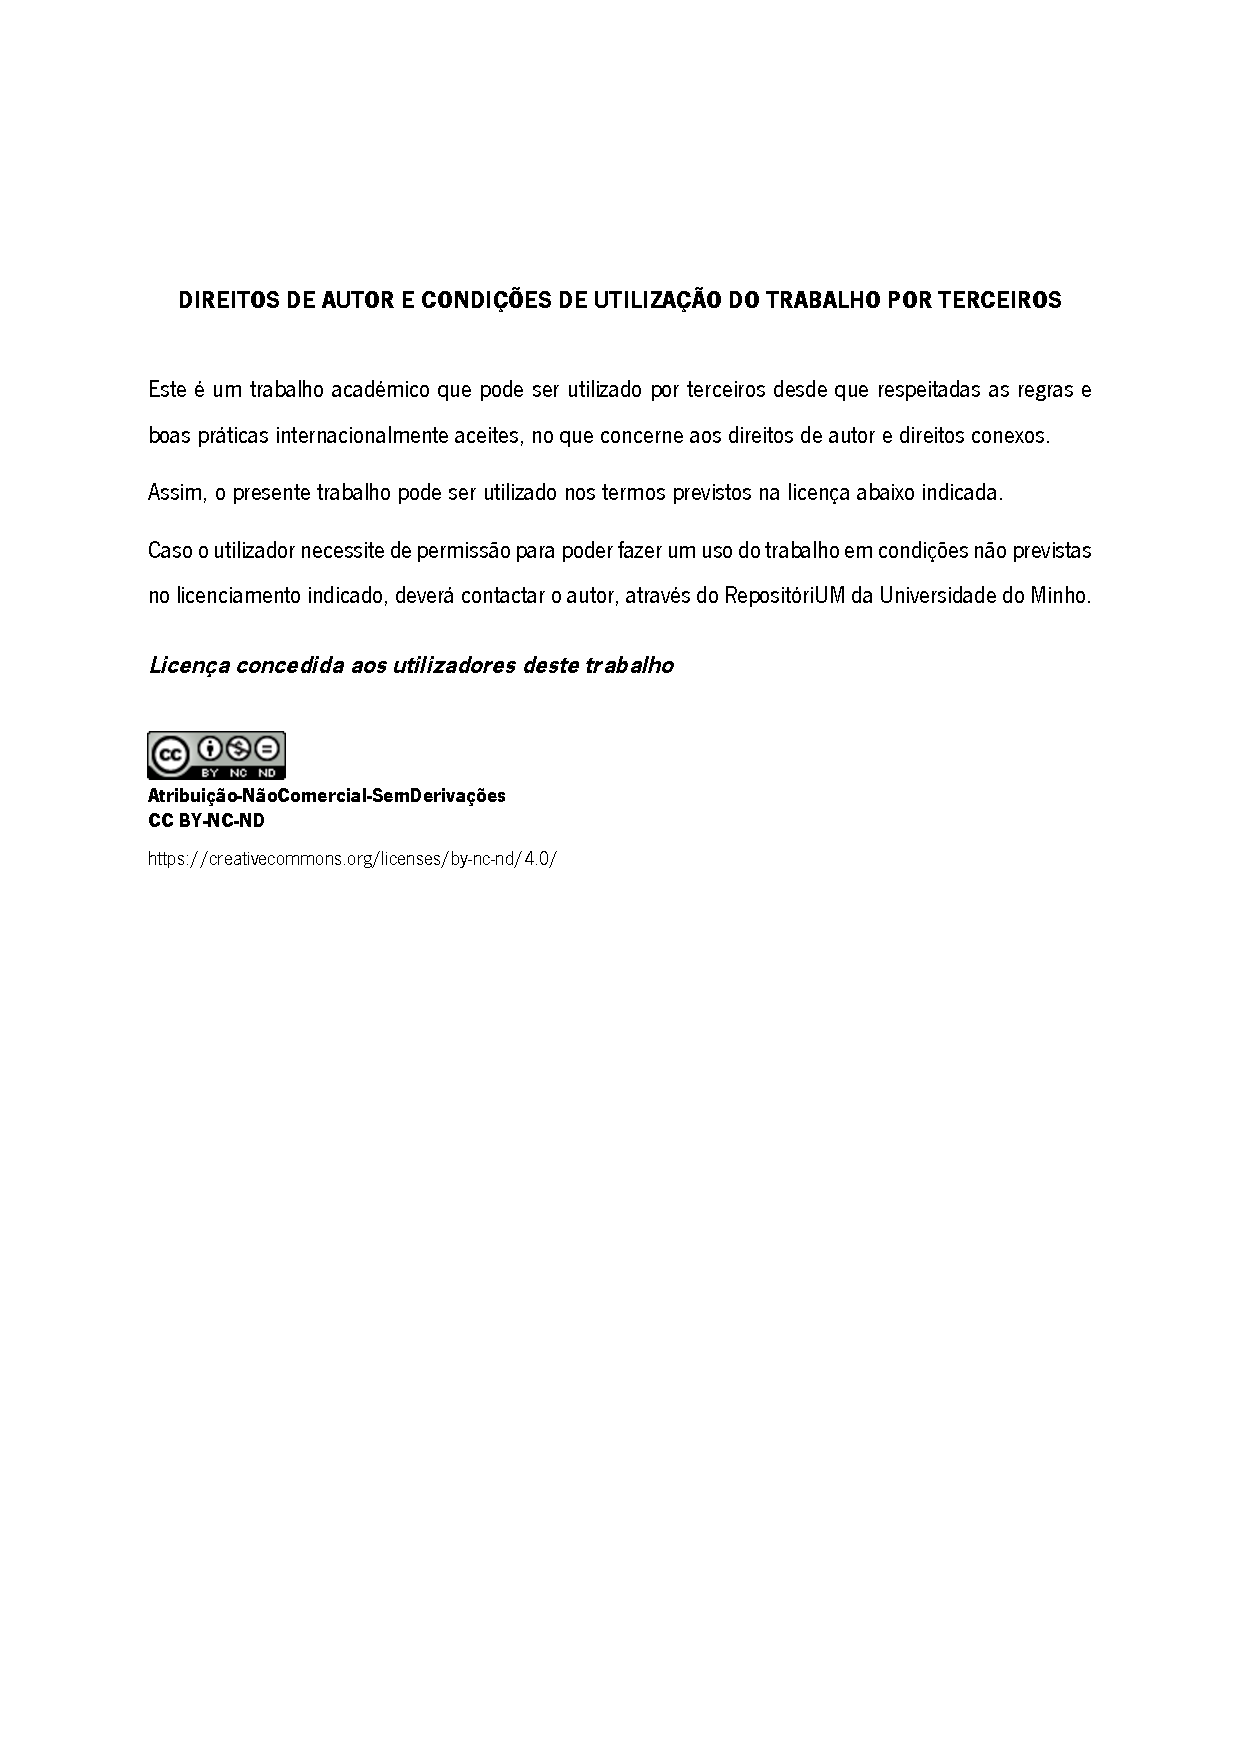
\includepdf[pages=-]{anexo3-license}
%  \cleardoublepage%
%%---------------------
%	% Add acknowledgements ----------------------------
%  \chapter*{Acknowledgements}
First and foremost, I would like to thank...
%%% Local Variables:
%%% mode: latex
%%% TeX-master: "../../dissertation"
%%% End:

%  %\chapter*{Acknowledgements}
%  %	Write acknowledgements here
%  \cleardoublepage%
%%---------------------
%  %
%  \KOMAoption{fontsize}{11.5pt}%
%	% Add abstracts (en,pt) ---------------------------
%  \chapter*{Abstract}
Functional design is the desirable and most sustainable method to design
products: by adding the material only where is strictly required to perform its
function, the resources usage is optimized, especially materials and
energy. However, functional design may dictate the usage of several materials or a combination of them to fulfill its goal, which is hindered by the
current manufacturing methodologies. An example of a class of
products where functional design is key is biomedical implants, like the hip implant.

% Keywords
\keywords{functional design, multimaterial, laser based additive manufacturing}
%%% Local Variables:
%%% mode: latex
%%% TeX-master: "../../dissertation"
%%% End:

%  %\chapter*{Abstract}
%	%Write abstract here (en) or import corresponding file	
%  \cleardoublepage%
%%
%  \KOMAoption{fontsize}{11pt}%
%  \chapter*{Resumo}
\selectlanguage{portuguese}%
O design funcional é o método mais desejável e sustentável de projetar
produtos: adicionando material somente é estritamente necessário para
a sua função, o uso de recursos é otimizado, especialmente materiais e

\keywordspt{design funcional, multimaterial, manufatura aditiva baseada em laser}
\selectlanguage{english}%
%%% Local Variables:
%%% mode: latex
%%% TeX-master: "../../dissertation"
%%% End:

%  %\chapter*{Resumo}
%	%Escrever aqui resumo (pt), ou importar respectivo ficheiro,
%  \cleardoublepage%
	% Summary Lists ------------------------------------
  % add toc and lists to TOC
  % src: https://tex.stackexchange.com/a/74440
%  \KOMAoption{fontsize}{12pt}%
  % TOC
  \phantomsection%
  \addcontentsline{toc}{chapter}{Contents}
  \tableofcontents%
  \cleardoublepage%
  % List of Figs
  \phantomsection%
  \addcontentsline{toc}{chapter}{List of Figures}
  \listoffigures%
  \cleardoublepage%
  % List of Tables
%  \phantomsection%
%  \addcontentsline{toc}{chapter}{List of Tables}
%  \listoftables
%  \cleardoublepage%
  % List of listings
  \phantomsection%
  \addcontentsline{toc}{chapter}{List of Listings}
  \lstlistoflistings%
  \cleardoublepage%
  % list of Acronyms
 % \phantomsection%
 % \addcontentsline{toc}{chapter}{List of Abbreviations}
 % \listofacronyms%
 % \cleardoublepage%
    %\printglossary[type=\acronymtype]%
    %\printglossary[type=\acronymtype]%
 %   \listofabbreviations%
  % List of symbols
  \phantomsection%
  \addcontentsline{toc}{chapter}{List of Symbols}
  \listofsymbols%
  \cleardoublepage%
%
	\thispagestyle{empty}
  %\newpage
	\pagenumbering{arabic}
  %\newpage
  %\setcounter{page}{0}
  %\pagenumbering{arabic}
  %\setcounter{page}{1}
 % 
  % making chapter pages with no header and footer
  \renewcommand*{\chapterpagestyle}{empty}
  %-------------- MAIN BODY CHAPTERS----------------------------------
  % Include the other files (\include adds a blank page between files)
  % - does not need the file extension
%  \KOMAoption{fontsize}{12pt}%
  \setlength{\unitlength}{1mm}
  %% 1,5 line spacing
  \renewcommand{\baselinestretch}{1.5}
%
  % For VIM to recognize the document syntax \begin{document} and \end{document}
% - However, the compilation will fail!! So don't forget to comment the
%   directives before compiling!!'
%
%\begin{document}
%
% CHAPTER - Introduction -------------------------
\chapter{Introduction}%
\label{ch:introduction}
The present work illustrates the application of the project meant to do for the course of Embedded Systems, required from the professors from \gls{esrg}.
This type of project begins with the establishment of what type of prototype do the students propose to do, followed for its implementation. This implementation needs to follow all the steps of the Waterfall Model in order to give students the capability to work the best way possible, either in group or in solo.

It should be noted, however, that there are some requirements and constraints gave by the professors which means that not everything is decided by the students. 
To have the capability of bypass them is one of the main characteristics of attending and working in engineering.
%
%  \vspace{-5mm}
  %
\section{Problem statement}%
\label{sec:prob-stat}
%The first step of the project is to clearly define the problem, as a result of
%the contract established between the client and the project team, yielding, in
%this case, the following project statement:
%
%``Design a remote control with three buttons that can
%remotely control the television (TV). It should be very
%light, powered by batteries and controls your TV via an
%infrared emitter. The TV has a built-in infrared receiver. A
%button on the remote control switches the TV on/off and
%will be labeled with the word "Power". The other two
%buttons are used to scroll up/down and select the available
%channels and they are labeled with the arrows up/down.''

%COVID pandemics presented a landmark on human interaction, greatly reducing the
%contact between people and surfaces. Thus, it is an imperative to provide people
%with contactless interfaces for everyday tasks. People redefined their
%purchasing behaviors, leading to a massive growth of the online
%shopping. However, some business sectors, like clothing or perfumes, cannot
%provide the same user experience when moving online.
%Therefore, one proposes to close that gap by providing a marketing digital
%outdoor for brands to advertise and gather customers with contactless
%interaction.
%
%Scenting marketing is a great approach to draw people into stores.
%Olfactory sense is the fastest way to the brain, thus, providing an exceptional
%opportunity for marketing~\cite{news-harvard} --- ``75\% of the emotions we generate on a daily basis are affected by smell. Next
%to sight, it is the most important sense we have''~\cite{lindstrom2006brand}.
%
%Combining that with additional stimuli, like sight and sound, can
%significantly boost the marketing outcome. Brands can buy advertisement space
%and time, selecting the videoclips to be displayed and the fragrance to be
%used at specific times, drawing the customers into their stores.
%
%Marketing also leverages from better user experience, thus, user interaction is
%a must-have, providing the opportunity to interact with the customer. In this
%sense, when users approach the outdoor a gesture-based interface will be
%provided for a brand immersive experience, where the user can take pictures or
%create GIFs with brand specific image filters and share them through their
%social media, with the opportunity to gain several benefits.

The first step of the project is to clearly define the problem, taking into
consideration the problem's context and motivation and exploiting the market opportunities.

\emph{The project consists of a \gls{mdo} with sound and
video display, and fragrance emission selected by the brands, providing a gesture-based interface for
user interaction to create pictures and \gls{gif}s, brand-specific, and share them on
social media.} It is comprised of several modes:
\begin{item-c}
\item \emph{normal mode (advertisement mode)}: the \gls{mdo} will provide
  sound, video and fragrance outputs.
\item \emph{interaction mode}: When a user approaches, the \gls{mdo} it will
go into interaction mode, turning on and displaying the camera feed and waiting
for recognizable gestures to provide additional functionalities, such as
brand-specific image filters.
\item \emph{sharing mode}: after a user take a picture or create a \gls{gif}, it
  can share it across social media.
\end{item-c}

Brands can buy advertisement space and time, selecting the videoclips to be
displayed and the fragrance to be used at specific times, drawing the customers
into their stores. Customers can be captivated by the combination of sensorial
stimuli, the gesture-based interaction, the immersive user experience provided
by the brands --- feeling they belong in a TV advertisement, and the opportunity
to gain several benefits, e.g., discount coupons.
%%% Local Variables:
%%% mode: latex
%%% TeX-master: "../../../dissertation"
%%% End:

\section{Context and motivation}
\label{sec:context-motivation}


%%% Local Variables:
%%% mode: latex
%%% TeX-master: "../../../dissertation"
%%% End:

\section{Market research}
\label{sec:market-research}
A Digital Outdoor is essentially a traditional outdoor advertising powered up by technology. 
The pros of a digital outdoor compared to a traditional one is mostly the way that it captivates the attention of consumers in a more dynamic way. 
It can also change its advertisement according to certain conditions, such as
weather and/or time. Some researches tells that the British public sees over 1.1
\gls{bn} digital outdoor advertisements over a week~\cite{digital-outdoor}, which can tell how much digital marketing is valued nowadays.

When talking about numbers, ``At the end of 2020, despite the Covid wipeout, the \gls{dooh} market was estimated to be worth \$41.06 \gls{bn}, but by 2026, nearly two out of three (65\%) advertising executives predict this will rise to between \$50 \gls{bn} and \$55 \gls{bn}. 
A further 16\% expect it to be worth between \$55 \gls{bn} and \$60 \gls{bn}, and 14\% estimate it will be even bigger''~\cite{outdoor-market}.

\begin{figure}[htb!]
\centering
    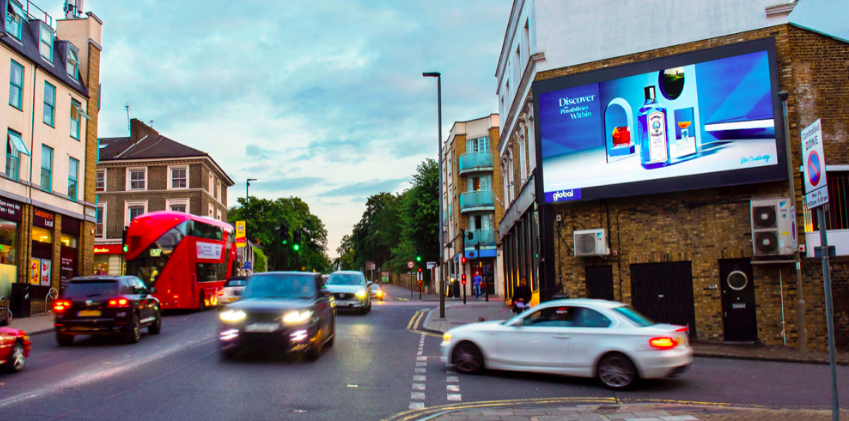
\includegraphics[width=0.7\columnwidth]{./img/DigitalOutdoor.png}
  \caption{Example of a Digital Outdoor, withdrawn from~\cite{digital-outdoor}}%
\label{fig:dig-outdoor}
\end{figure}

Scent market is the art of taking a company's brand identity, marketing messages, target audience and creating a scent that amplifies these values. 
That's because ``a scent has the ability to influence behavior and trigger memories almost instantaneously. When smell is combined with other marketing cues, it can amplify a brand experience and establish a long lasting connection with consumers''~\cite{scent-market}.

Ambient scent uses fragrance to enhance the experience of consumers with different purposes, whereas scents in scent branding are unique to each company's identity.
According to a Samsung study: ``when consumers were exposed to a company scent, shopping time was increased by 26\% and they visited three times more product categories'' ~\cite{scent-stats}.
Also, ``the digital scent technology market is expected to grow from \$1.0 \gls{bn} in 2021 to \$1.5 \gls{bn} by 2026, at a \gls{cagr} of 9.2\%.''~\cite{scent-money}.

\begin{figure}[htb!]
\centering
    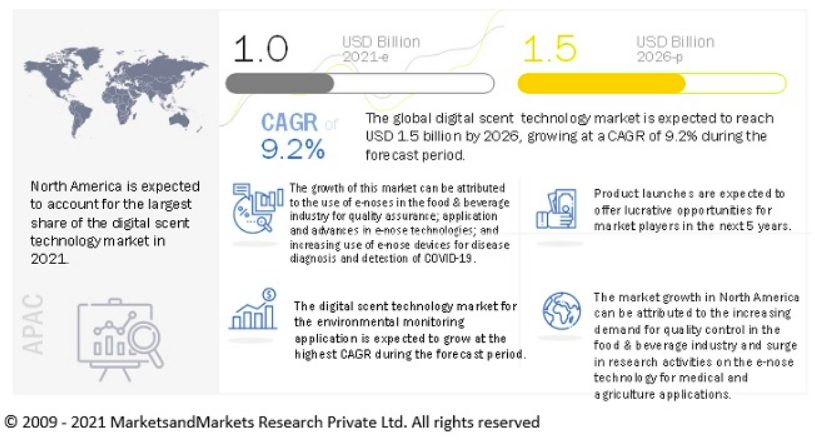
\includegraphics[width=0.9\columnwidth]{./img/scentstats.png}
  \caption{Attractive Opportunities in the Digital Scent Technology Market, withdrawn from~\cite{scent-money}}%
\label{fig:scent-stat}
\end{figure}

The market growth can be attributed to several factors, such as expanding application and advancements in e-nose technologies, increasing use of e-nose devices for disease diagnostic applications, emerging \gls{rd} activities to invent e-nose to sniff out COVID-19, and rising use of e-nose in food industry for quality assurance in production, storage, and display.

% Remote material (side by side)
%\begin{figure}[htb!]
%  \centering
  %
%  \begin{subfigure}{.4\textwidth}
%  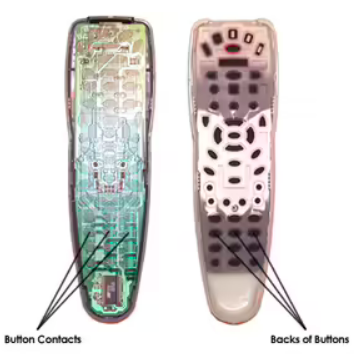
\includegraphics[width=\textwidth]{img/remotematerial1.png}%
  %\caption{KUKA's original position}%
  %\label{fig:ptp-test-orig}
%\end{subfigure}
%
 % \begin{subfigure}{.4\textwidth}
  %  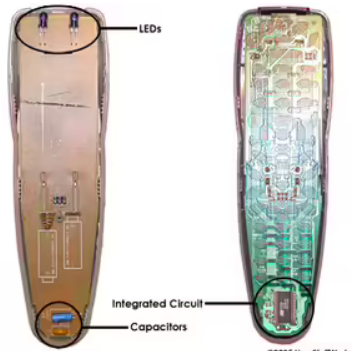
\includegraphics[width=\textwidth]{img/remotematerial2.png}%
%  \caption{KUKA's final position}%
%  \label{fig:ptp-test-final}
%\end{subfigure}
%
%  \caption{TV Remote control bill of materials, withdrawn from~\cite{remotematerial}}%
%  \label{fig:remotemat}
%\end{figure}
%

%%% Local Variables:
%%% mode: latex
%%% TeX-master: "../../../dissertation"
%%% End:

\section{Project goals}%
\label{sec:project-goals}
The project aims to develop a \gls{cps} for multi-sensorial marketing with
contactless user interaction. The key goals identified and the respective path
to attain them are:
\begin{enum-c}
\item \emph{devise a device with audio and video outputs, as well as fragrance
    diffusion}: understand audio and video streaming and study fragrance
  nebulizer technologies.
\item \emph{create a contactless user interface based on gestures through
    computer vision}: identify user gestures through computer vision and match them to interface
  callbacks; a virtual keyboard may be required for user input.
\item \emph{devise a distributed architecture to convey brand advertisement
  information to the local device}: understand distributed architectures and
apply them for optimal data flow; create a remote client-server model to convey
information from the brands to the device through remote cloud database
services; devise adequate data frames to convey information to the local device;
create a local server to respond to the remote server requests.
\item \emph{apply facial recognition to the camera feed and subsequently apply
  image filters specific to each brand}: understand facial recognition
algorithms and apply them to the camera feed; apply image filters on top of the
identified faces through a specialized \gls{api}.
\item \emph{enable image and GIFs sharing to social media for increased brand
    awareness}: understand how to use social media APIs for media sharing.
\end{enum-c}
%
%%% Local Variables:
%%% mode: latex
%%% TeX-master: "../../../dissertation"
%%% End:

\section{Report Outline}
\label{sec:report-outline}
This report is organised as follows:
\begin{itemize}
%\item In Chapter~\ref{ch:state-art}, the state of the art of remote controlled
%vehicles is presented.
%\item In Chapter~\ref{ch:theor-found} lays out the theoretical foundations for
%  project development,
%  namely the project development methodologies and associated tools, and the
%  communications technologies.
%\item In Chapter~\ref{ch:requirements-specs} are identified the key requirements
%  and constraints the system being developed must meet from the end-user
%  perspective (requirements) and, by defining well-established boundaries within
%  the project resources (time, budget, technologies and know-how), the list of
%  spefications is obtained.
%\item After defining the product specifications, the solutions space is explored
%  in Chapter~\ref{ch:analysis}, providing the rationale for viable solutions and
%  guiding the designer towards a best-compromise solution, yielding the
%  preliminary design and the foreseen tests to the specifications.
%\item The preliminary design is further refined in Chapter~\ref{ch:design} and
%  decomposed into tractable blocks (subsystems) which can be designed
%  independently and assigned to different design teams, allowing the transition
%  to the implementation phase.
%\item Next, in Chapter~\ref{ch:implementation}, the design solution is
%  implemented into the target platforms.
%\item Then, in Chapter~\ref{ch:testing}, the implementation is tested at the
%  subsystem level (unit testing) and system level (integrated testing),
%  analysing and comparing the attained performance with the expected one.
%\item After product testing, in Chapter~\ref{ch:verif-valid}, the specifications
%  must be verified and validated by an external agent.
%  subsystem level (unit testing) and system level (integrated testing),
%  analysing and comparing the attained performance with the expected one.
%\item Chapter~\ref{ch:conclusion} gives a summary of this report as well as
%  prospect for future work.
\item Lastly, the appendices (see Section~\ref{ch:Append}) contain detailed
  information about project planning and development.
\end{itemize}


%%% Local Variables:
%%% mode: latex
%%% TeX-master: "../../../dissertation"
%%% End:

%
%%% Local Variables:
%%% mode: latex
%%% TeX-master: "../../../dissertation"
%%% End:

  \setcounter{table}{0}
  \setcounter{figure}{0}
%  
  \chapter{Target Acquisition}%
\label{ch:target-acquisition}
An autonomous mobile robot must be able to navigate to a target
position. Information about the target position can be provided by \textit{a
  priori} knowledge of the target coordinates --- $\gls{xtar}, \gls{ytar}$ --- or the
robot computer vision system may indicate the direction of the target (see
Fig.~\ref{fig:fig1}).
%
% Fig 1
\begin{figure}[!hbt]
\centering
    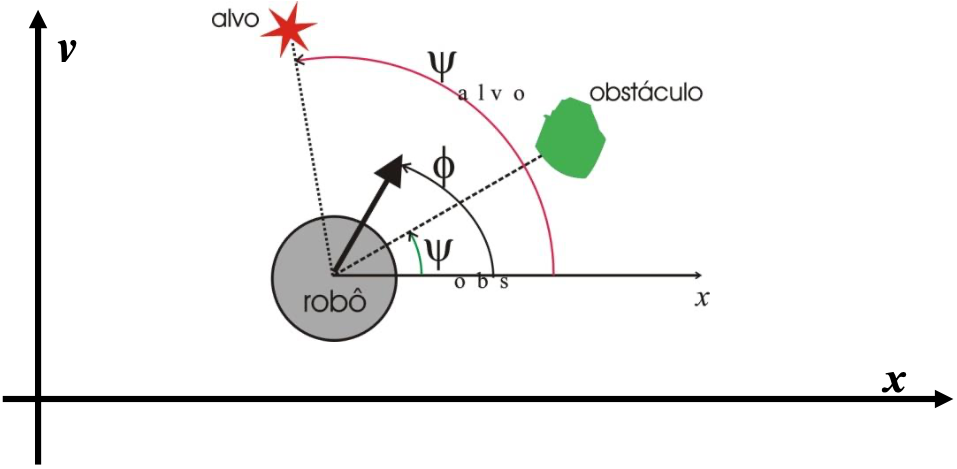
\includegraphics[width=0.6\textwidth]{./img/fig1.png}
  \caption[Target acquisition heading angle referencing to external world
  axes]{Target acquisition heading angle referencing to external world axes: The angle by which the robot `sees', $\gls{psi-tar}$, the target in
    relation to external world axes may be yielded by the robot's computer
    vision system or may be computed if the target coordinates ($x_{tar},
    y_{tar}$) are known and one has an estimative of the position of the robot
    ($x_{robot}, y_{robot}$)}%
\label{fig:fig1}
\end{figure}

The target acquisition behavior can be yielded by dynamic systems for the
heading direction and linear velocity:
%
\begin{equation}
  \label{eq:3}
  \frac{d \phi}{dt} = f_{tar}(\phi{,} \psi _{tar}) + f_{stoch}
\end{equation}
\begin{equation}
  \label{eq:4}
\frac{dv}{dt} = g_{tar} (v)
\end{equation}

The term $\gls{ftar}$ of the vectorial field in the equation~(\ref{eq:3}) may have
the nonlinear form:
\begin{equation}
  \label{eq:5}
f_{tar}(\phi{,} \psi _{tar}) = - \lambda _{tar} \sin (\phi - \psi _{tar})
\end{equation}
%
where $\gls{lambda-tar}$ is a parameter that defines the magnitude of the
`attraction force' the target exerts over the robot and $\psi _{tar}$ is the
direction the robot `sees' the target.

The term $\gls{fstoch}$ of the vectorial field in the equation~(\ref{eq:3})
represents the stochastic force that must be present to ensure escape from
repellers within a limited time:
\begin{equation}
  \label{eq:6}
f_{stoch} = \sqrt{Q} \varepsilon _{n}
\end{equation}
modelled as Gaussian white noise, $\gls{varepsilon-n}$, of unit variance, so that
$\gls{Q}$ is the effective variance of the force~\cite{bicho2000dynamic}.

\section{Analytical study of nonlinear dynamic system defined by
  Eqs. (\ref{eq:3}) and (\ref{eq:5})}%
\label{sec:analyt-study-tar-nonl}
In this section, an analytical study of the dynamic system defined by
Eqs. (\ref{eq:3}) and (\ref{eq:5}) is performed. The fixed points of this
dynamic system are determined and its stability is assessed, thus leading to
successfull positioning of the attractor for the heading direction. Then, the phase
portraits and bifurcation diagram are drawn, yielding the range of admissible
values for the magnitude of the attractor.

\subsection{Fixed points of the dynamic system}%
\label{sec:fixed-points-dynamic}
The fixed points of the dynamic system are the values, $\gls{phi-star}$, for which the
state of the system does not change, i.e., $f_{tar}(\phi^*) = 0$. Once placed at
a fixed point, the system remains fixed in that state ($d \phi / dt = 0$), hence
also named as constant solutions of the dynamic system. Graphically, the fixed
points correspond to the intersection of the function $f(\phi)$ with the $\phi$
axis.

Fig.~\ref{fig:1-1-fixed-points} illustrates the determination of the fixed
points of the dynamic system, given by Eq.~(\ref{eq:7}),yielding the general solution:
$\phi^* = \psi_{tar} + k \pi$. As the heading direction $\phi \in [0, 2 \pi[$
represents a circular phase space, the solutions can be limited to $\phi_1^* =
\psi_{tar}, \phi_2^* = \psi_{tar} + \pi$.
\begin{equation}
  \label{eq:7}
  \left. \frac{d \phi}{dt}\right|_{\phi = \phi^*} = f_{tar}(\phi^*) = 0
\end{equation}
% fixed points
\begin{figure}[!hbt]
\centering
    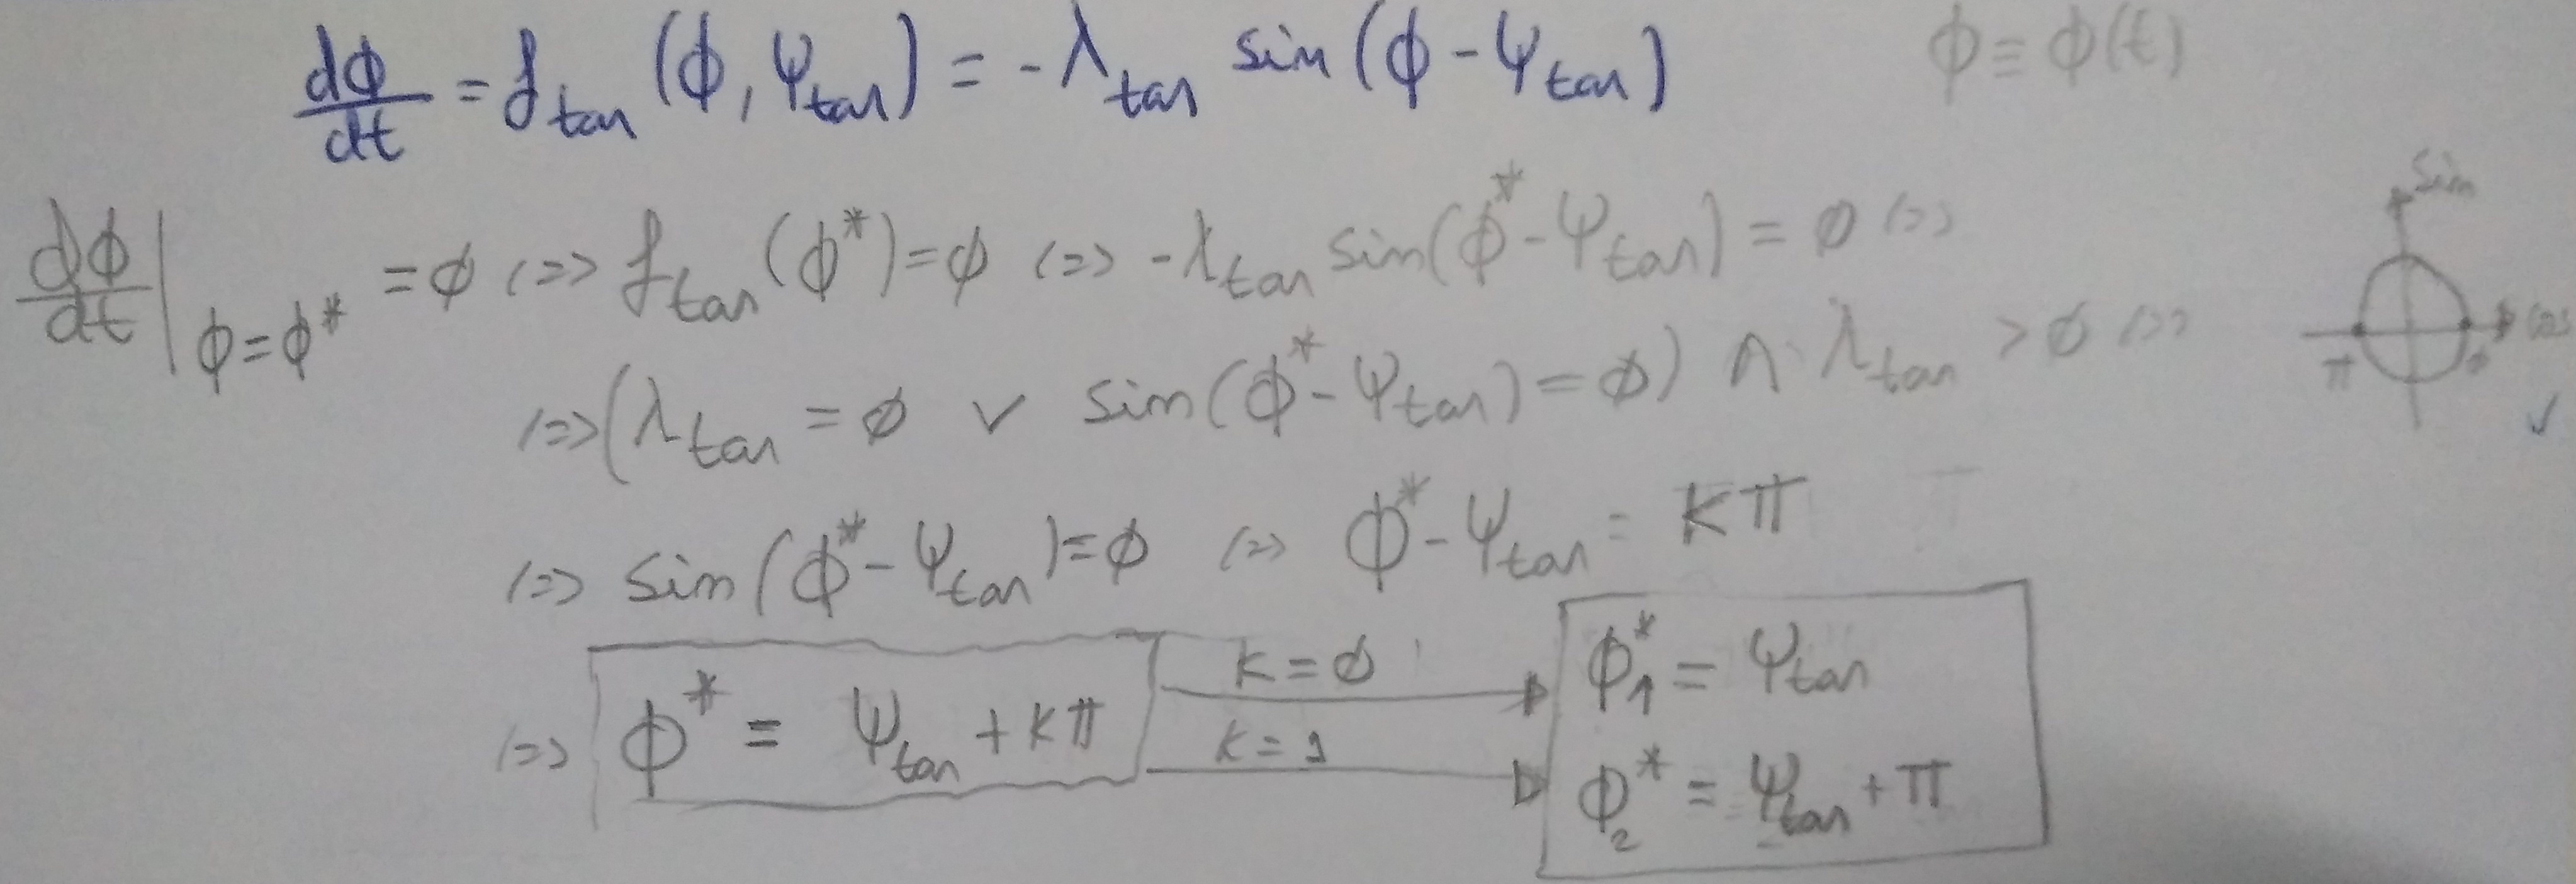
\includegraphics[width=1.0\textwidth]{./img/1-1-fixed-points.jpg}
  \caption{Target acquisition behavior: Determination of fixed points}%
\label{fig:1-1-fixed-points}
\end{figure}
% 
\subsection{Stability of the fixed points and relaxation time}%
\label{sec:stab-fixed-points}
The determination of the stability of fixed points is useful to understand its
qualitative behavior. It can be determined analytically using Eq.~(\ref{eq:8}),
or infered graphically by observing the slope of $f_{tar}(\phi)$ at the fixed
points.
%
\begin{equation}
  \label{eq:8}
  m = \left. \frac{d f_{tar}(\phi)}{d \phi}\right|_{\phi = \phi^*}
\end{equation}

Three cases arise, depending on the sign of $\gls{m}$:
\begin{enumerate}
\item $m < 0$: $\phi^*$ is an asymptotically stable state, i.e., an attractor;
\item $m > 0$: $\phi^*$ is an unstable state, i.e., an repeller;
\item $m = 0$: nothing can be concluded about $\phi^*$ using the analytical
  method. The graphical method must be used.
\end{enumerate}

The relaxation time, $\gls{tau-tar}$, corresponds to the required time for the system state be
significantly attracted to the asymptotically stable state when it is in the
vicinity of this fixed point. It can be determined from the inverse of the slope
on the vicinity of the fixed point, as given by Eq.~(\ref{eq:9}):
\begin{equation}
  \label{eq:9}
  \tau_{tar} = \frac{1}{| f'(\phi^*) |}
\end{equation}

Fig.~\ref{fig:1-2-stability-fixed-points} illustrates the assessment of the
stability of the fixed points and the relaxation time. It can be observed that
the analytical method provides $m_1 = - \lambda_{tar}, m_2 = \lambda_{tar}$.
Thus, for the attractor to be placed in the target direction, i.e. $\phi_1^* =
\psi_{tar}$, and an repeller in the opposite direction, i.e., $\phi_2^* =
\psi_{tar} + \pi$ as expected, $\lambda_{tar} > 0$.
This way the robot can rapidly divert from the repeller and move to the
attractor direction. The relaxation time is inversely proportional to the local
time constant, i.e., inversely proportional to the magnitude of the attractive
force-let $\tau_{tar} = 1/\lambda_{tar}$ s.
%
% stability
\begin{figure}[!hbt]
\centering
    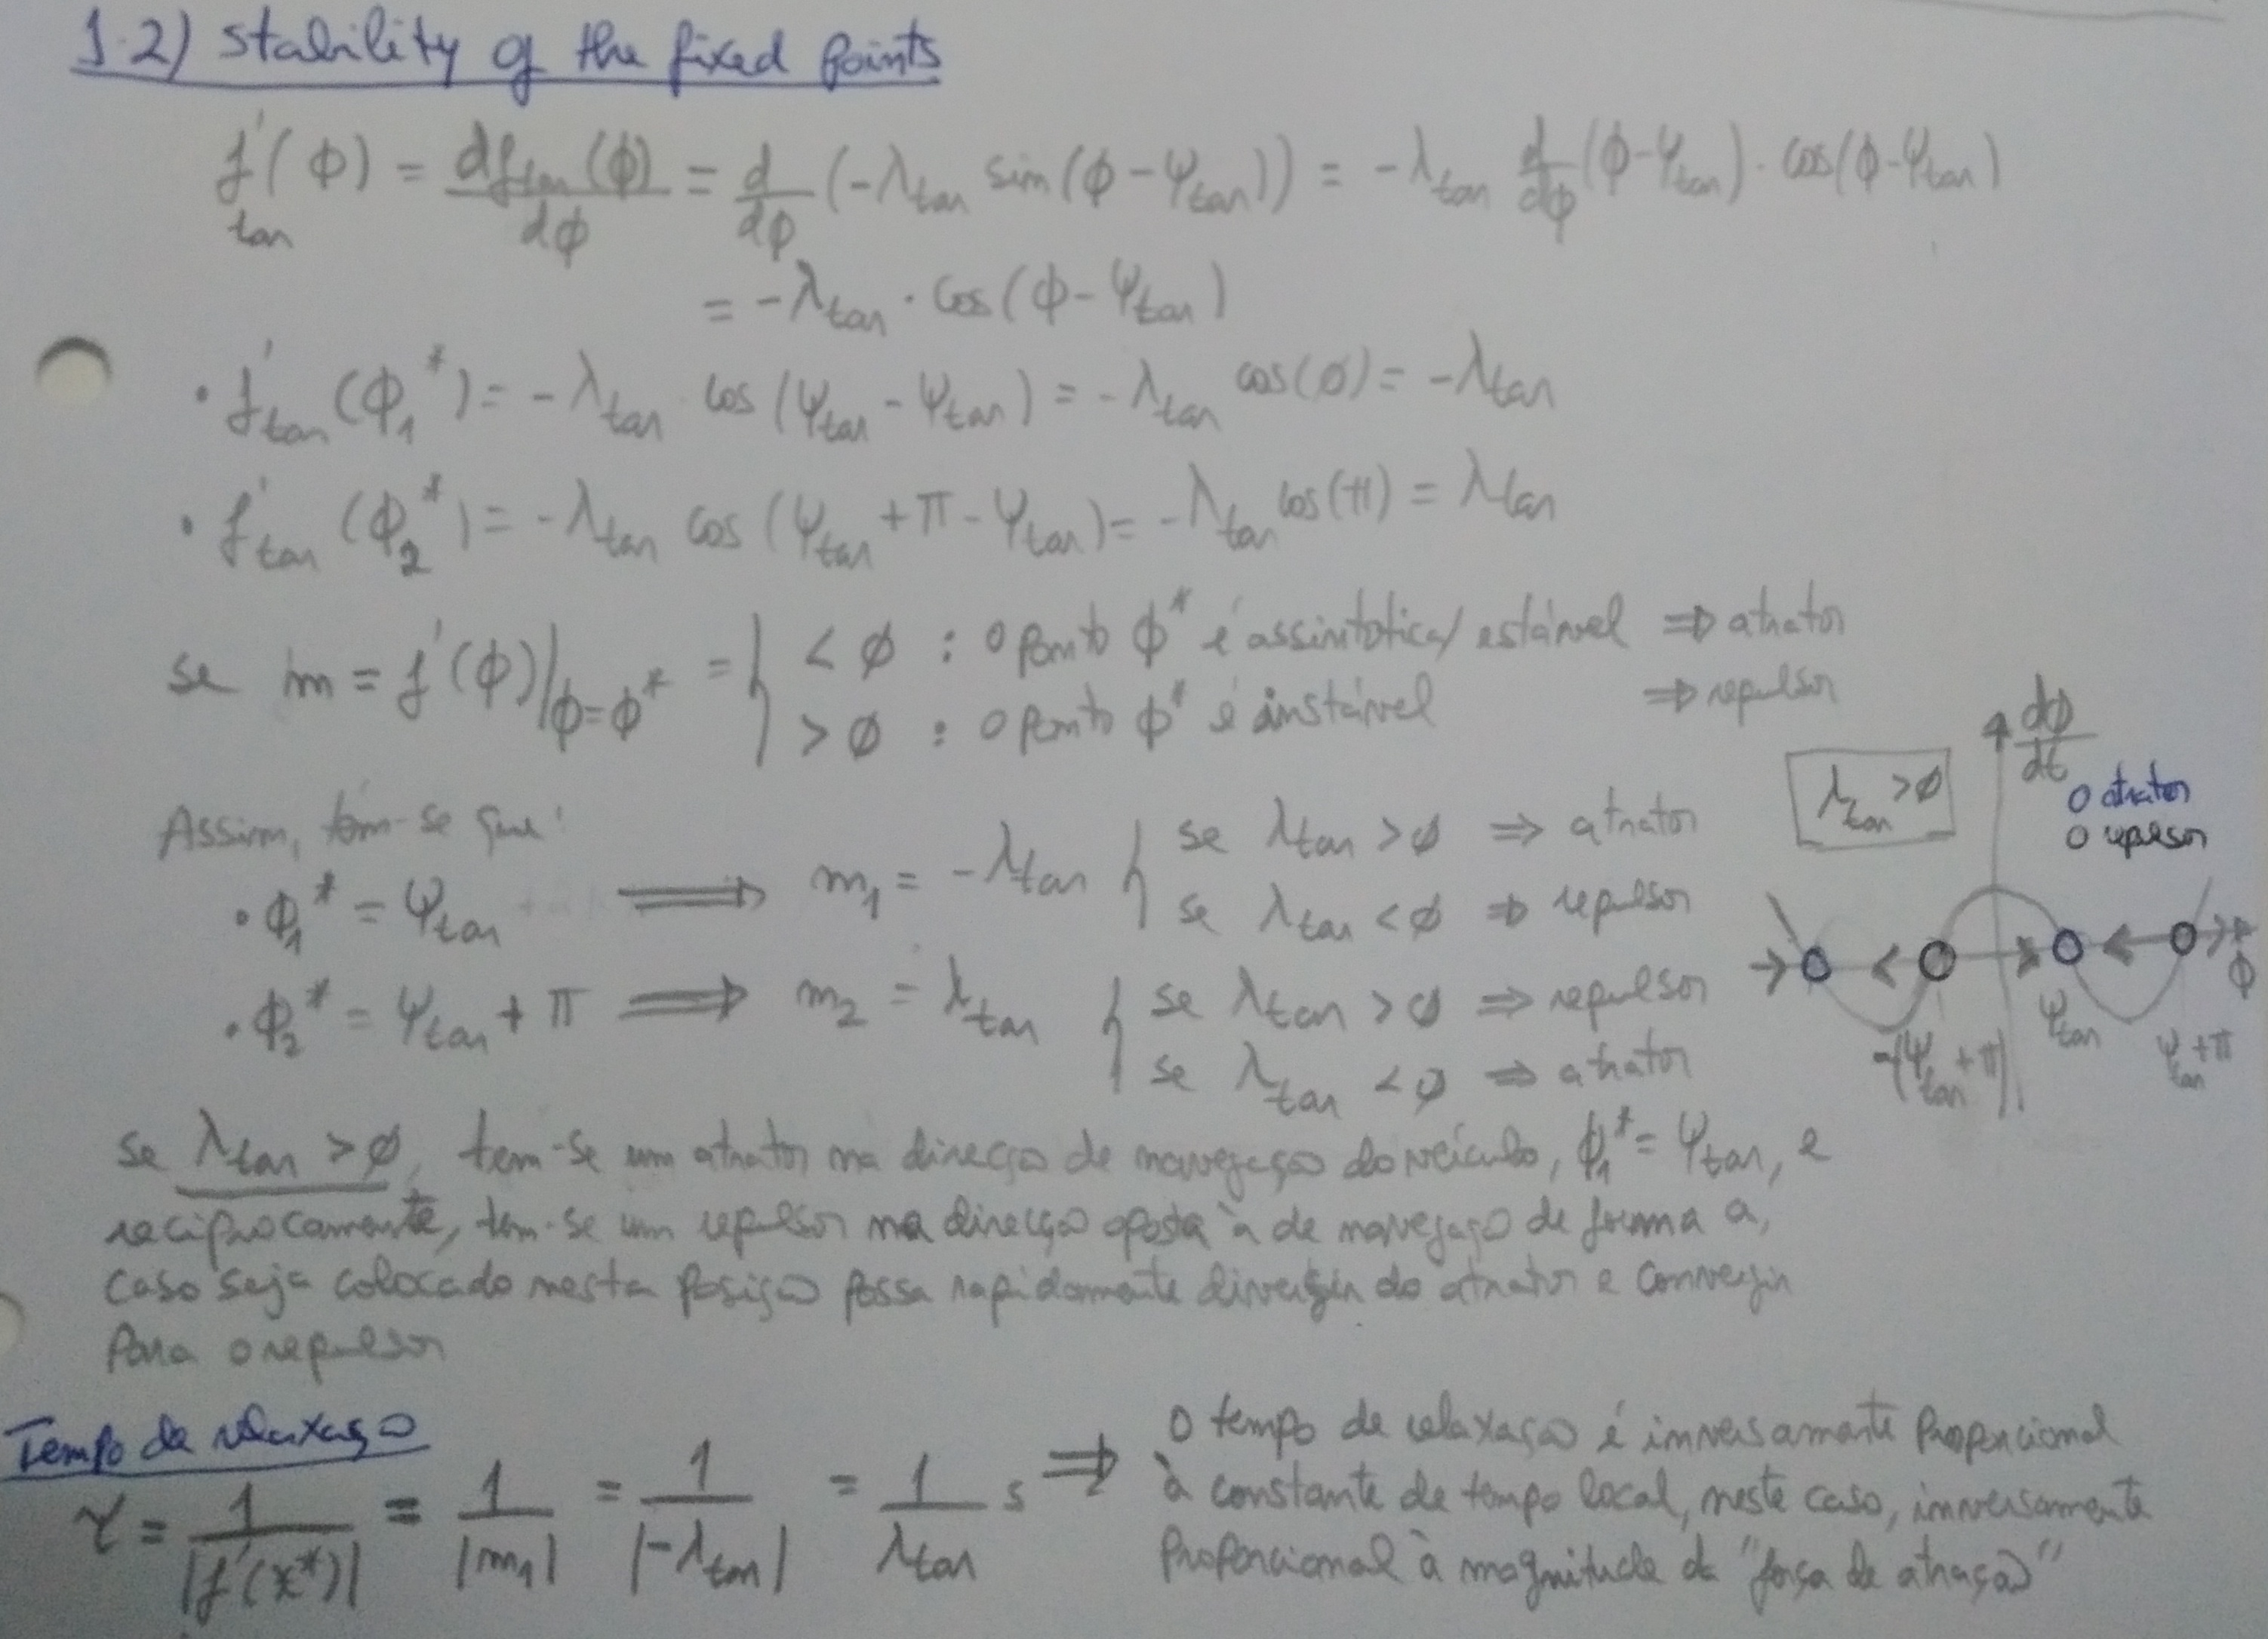
\includegraphics[width=1.0\textwidth]{./img/1-2-stability-fixed-points.jpg}
  \caption{Target acquisition behavior: Stability of fixed points and relaxation time of the attractor}%
\label{fig:1-2-stability-fixed-points}
\end{figure}
%
\subsection{Phase portraits}%
\label{sec:phase-portraits}
The phase portrait of a dynamic system consists in a graphical representation
that shows all its qualitatively different trajectories. The fixed points are
represented as circles and the evolution direction of the state $\phi$ as the
time progresses is indicated by arrows --- convergent arrows to attractors and
divergent arrows from repellers.

Fig.~\ref{fig:1-3-phase-portraits} depicts the possible phase portraits for the
target acquisition dynamic system, depending on the sign of the parameter
$\lambda_{tar}$:
\begin{itemize}
\item $\lambda_{tar} > 0$: an attractor is placed in the target direction and a
  repeller is placed in the opposite direction. This represents the intended
  behavior for the system.
\item $\lambda_{tar} < 0$: a repeller is placed in the target direction and a
  attractor is placed in the opposite direction. This represents an undesired
  behavior for the system.
\end{itemize}
%
% phase-portraits
\begin{figure}[!hbt]
\centering
    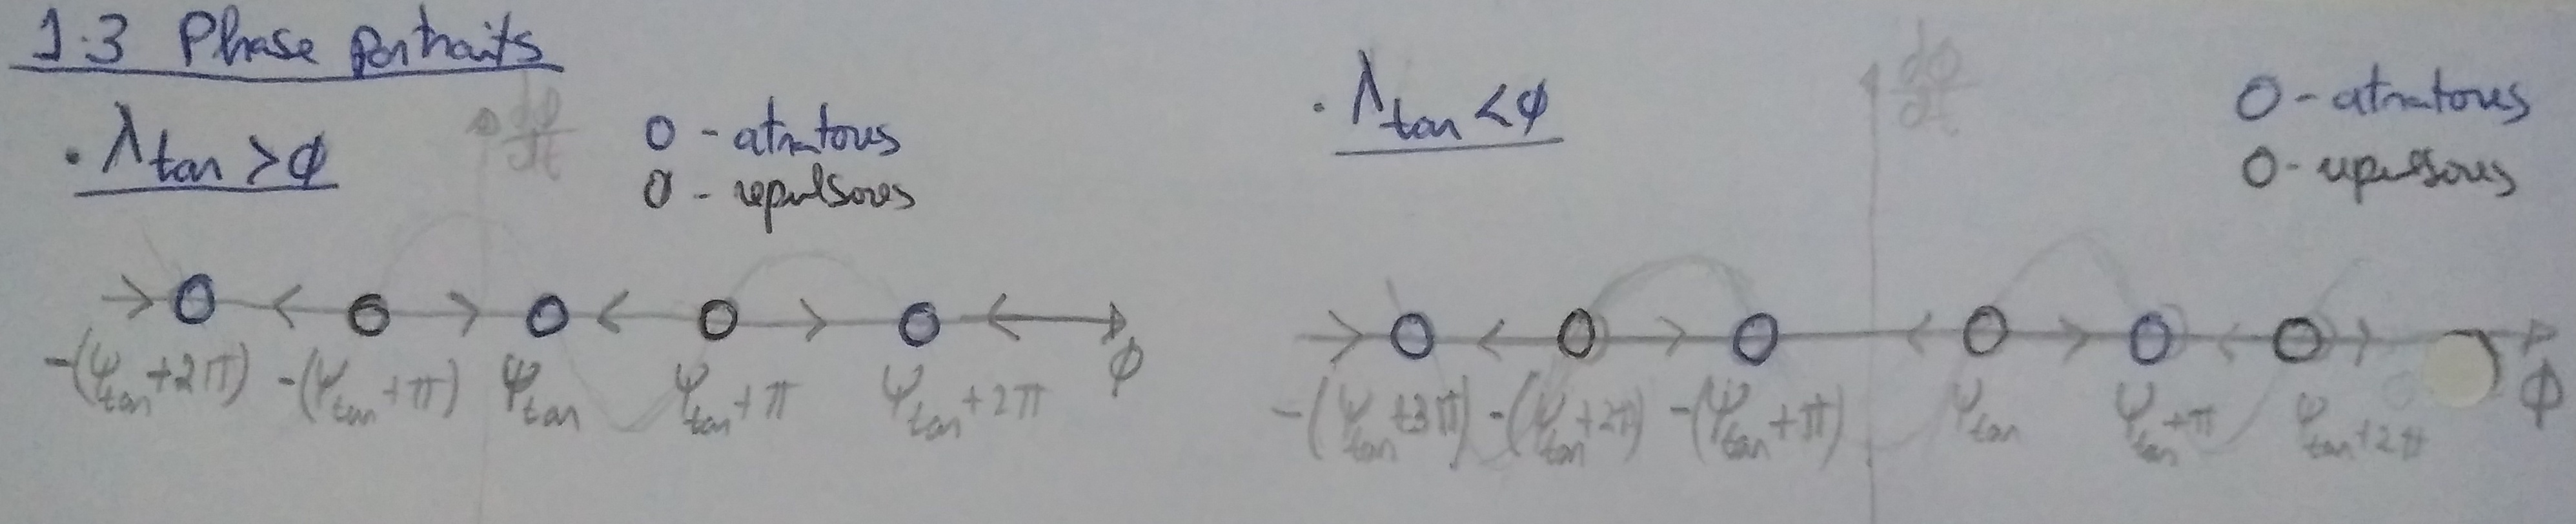
\includegraphics[width=1.0\textwidth]{./img/1-3-phase-portraits.jpg}
  \caption{Target acquisition behavior: Phase portraits}%
\label{fig:1-3-phase-portraits}
\end{figure}
%
\subsection{Bifurcation diagram}%
\label{sec:bifurcation-diagram}
Bifurcations arise as the qualitative behavior of the system changes, i.e., the
number, nature and/or stability of the fixed points changes. A bifurcation point
is the value of the parameter for which the qualitative change of the system
behavior occurs. The bifurcation diagram consists in a graphical representation
of the fixed points and respective stability as a function of a parameter of
$f(\phi)$.

Fig.~\ref{fig:1-4-bifurcation-diag} depicts the bifurcation diagram for the
target acquisition dynamic system, as a function of the parameter $\lambda_{tar}$
for both fixed points --- $\phi_1^* = \psi_{tar}, \phi_2^* = \psi_{tar} - \pi,
\psi_{tar} > 0$:
\begin{itemize}
\item $\lambda_{tar} < 0$: the fixed point $\phi_1^*$ is unstable and
  $\phi_2^*$ is asymptotically stable.
\item $\lambda_{tar} > 0$: the fixed point $\phi_1^*$ becomes asymptotically stable and $\phi_2^*$ is unstable.
\end{itemize}
%
$\lambda_{tar} = 0$ is a bifurcation point. This represents a transcritical bifurcation as there is an exchange in the
stability between fixed points.
%
% Bifurcation diagram
\begin{figure}[!hbt]
\centering
    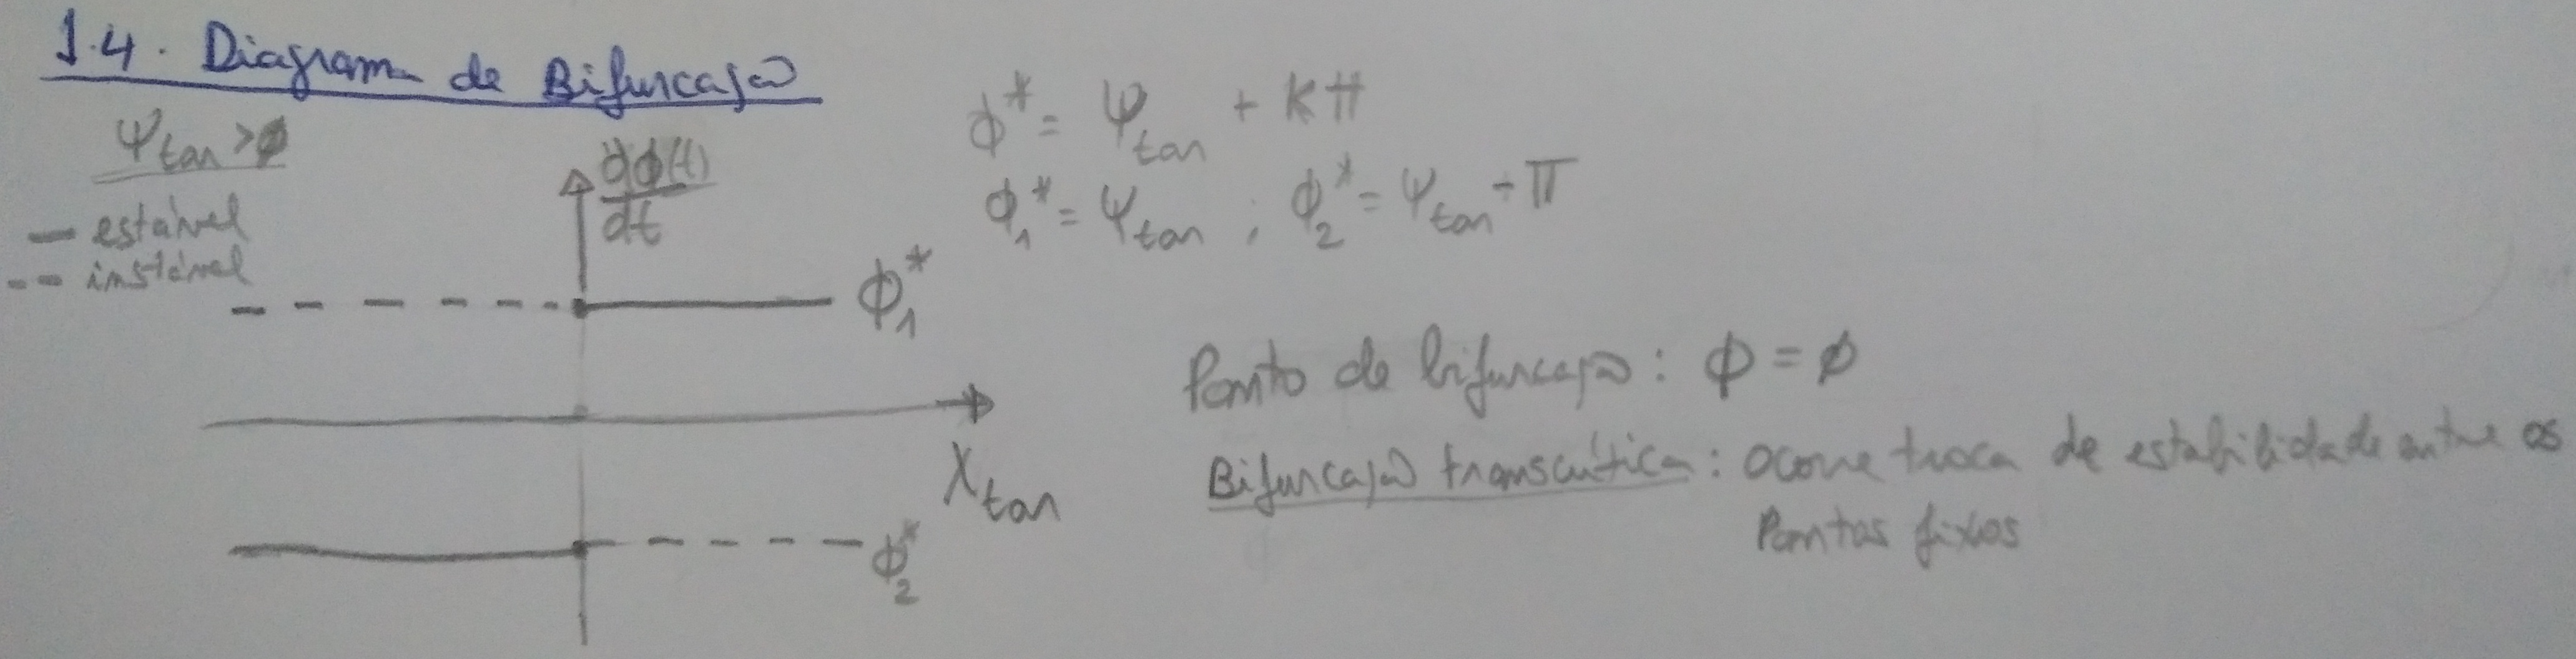
\includegraphics[width=1.0\textwidth]{./img/1-4-bifurcation.jpg}
  \caption{Target acquisition behavior: Bifurcation diagram}%
\label{fig:1-4-bifurcation-diag}
\end{figure}
%
\subsection{Range of values for $\lambda _{tar}$}%
\label{sec:range-tar}
For the target acquisition behavior, i.e. for the robot to move the target, an
attractor must be placed in the direction of the target, thus $\phi_1^* =
\psi_{tar}$ must be an asymptotically stable state of the system and consequently $\lambda_{tar} > 0$. 
\section{Implementation of nonlinear dynamic system defined by
  Eqs. (\ref{eq:3}) and (\ref{eq:5})}%
\label{sec:implem-study-tar-nonl}
In this section is demonstrated the implementation of the nonlinear dynamic
system for the heading direction. Additionally, a linear dynamic system for
the linear velocity of the robot is also implemented.

The first step of the implementation is to convert the first order differential
equation into an algebraic recursive equation by applying the forward Euler's
method in a discrete form:
\begin{equation}
  \label{eq:10}
  \phi(t + \Delta t) = \phi(t) + \Delta t f(\phi), \qquad \phi(t_0) = \phi_0
\end{equation}
where $\gls{delta-t}$ is the Euler's step --- the incremental timestep applied to
the recursive equation. For smooth variation of the heading direction the
Euler's step must be significantly smaller than the minimum time constant (in
this case, the relaxation time), i.e.: $\Delta t \ll \tau _{tar}$. As a rule of
thumb: $5 \Delta t \le \tau_{tar} \le 10 \Delta t$.

Next, the direction of the target, $psi_{tar}$ must be determined, based on the
known target coordinates and the robot's estimated coordinates with respect to
the external reference axis, respectively, $(x_{tar},y_{tar})$ and $(\gls{xrobot},
\gls{yrobot})$, taking into consideration the quadrant, as follows (see Fig.~\ref{fig:fig1}):
\begin{equation}
  \label{eq:11}
 \psi_{tar} = atan2 \Big(\frac{y_{tar} - y_{robot}}{x_{tar} - x_{robot}}\Big)
\end{equation}
It is important to note that the target acquisition dynamics is dependent
on the calibration of the heading direction of the robot in respect to the
external reference axis to accurately locate it.

Then, both components of the dynamic system, $f_{tar}$ and $f_{stoch}$ can be
computed using Eqs.~(\ref{eq:5}) and~(\ref{eq:6}) and added, yielding the
complete dynamic system as given by Eq.~(\ref{eq:3}). Next, the angular velocity
of the vehicle can be determined, noting that $\omega _{robot} = d \phi /dt$,
i.e., equal to the complete vector field.

Finally, linear velocity is defined, and, if desired a stop criterion for the
distance to target. Then, the values of the angular and linear velocities of the
robot can be passed as setpoints to the low-level code responsible for
controlling these control variables.

Summarizing, the pseudocode for the target acquisition behavior is as follows:
\begin{enumerate}
\item Initialize robot: retrieve simulation timestep and robot characteristics
\item Set initial values (linear and angular velocities) and set robot's initial
  pose ($x_{robot}, y_{robot}, \phi_{robot}$)
\item Initialize target
\item While target <= targetNr
  \begin{enumerate}
  \item Exchange information with the simulator
  \item Get vehicle's pose, target position and simulation timestep
  \item Trigger a simulation step
  \item Processing step
    \begin{enumerate}
    \item Set parameters values: $\tau_{tar}, \lambda_{tar}, Q$
    \item Compute $\psi_{tar}$
    \item Compute $f_{tar}$ and $f_{stoch}$
    \item Compute resultant vector field $f_{total}$ and assign it to angular
      velocity
    \item Set linear velocity
    \item Define stop criterion for target distance (if desired)
    \end{enumerate}
  \item View dynamics: plot the target acquisition dynamics
  \item Set robot's angular and linear velocities
  \end{enumerate}
\item Terminate simulation and cleanup
\end{enumerate}

As a result, the following generic Matlab code was implemented (Listing~\ref{lst:program-dyn-tar}):
% program_dyn_tar.m (generic)
\lstinputlisting[language=matlab, caption={Generic implementation of target
  acquisition behavior (not tuned)},label=lst:program-dyn-tar,
style=custom-matlab]{./listing/program_dyn_tar.m}%

Several scenarios have been simulated in CoppeliaSim/Matlab --- scenario
\texttt{MobileRobotDyn\_tar.ttt} --- for different linear velocity conditions namely:
\begin{enumerate}
\item Robot with rotational motion only: v = 0 m/s;
\item Robot moving at constant speed: v = K m/s;
\item Robot moving at a velocity defined by a vectorial field;
\end{enumerate}
%
\subsection{Rotational motion only}%
\label{sec:robot-initially-at}
In this first scenario, one considers only the existence of the rotational
motion of the robot in respect to its center of mass, i.e., v = 0 m/s. The
parameters were tuned to guide the robot for the desired target direction.

The scenario \texttt{MobileRobotDyn\_tar.ttt} was loaded in CoppeliaSim and the
robot was placed in the opposite direction of the target (worst case scenario),
as illustrated in Fig.~\ref{fig:tar-2-1-arena}. Then, the initial values of angular
and linear velocities were set and the parameters were tuned as indicated in
Listing~\ref{lst:program-dyn-tar-2-1}:
\begin{itemize}
\item $v_{robot} = 0$: robot does not exhibit translational motion.
\item $\tau_{tar} = 5 \Delta t$: minimum value to ensure forward Euler's method convergence.
\item $Q = 0.01$: sufficient effective variance of the Gaussian white noise to
  enable qualitative differences in the behavior (turn left/right).
\end{itemize}
% program_dyn_tar.m (generic)
\lstinputlisting[language=matlab, caption={Target acquisition behavior: Parameter tuning for v = 0 m/s},label=lst:program-dyn-tar-2-1,
style=custom-matlab]{./listing/program_dyn_tar_2_1.m}%

Fig.~\ref{fig:tar-2-1} illustrates the target acquisition dynamics in the final
condition. Initially, the heading direction, $\phi$, sits in a repeller $\phi =
50 + 180 ^{\circ}$ (positive slope). The heading direction diverts from this fixed point as it
represents an unstable state and tries to redirect to the attractor (turning in
clockwise direction) located at
$\phi = 50 ^{\circ}$ (negative slope). When it reaches this asymptotically
stable state the robot remains there, as intended. This validates the behavior
of orientation to the target.

Additionally, it is important to note the effect of the stochastic force: in
some occasions the robot follows a different trajectory for target orientation
by turning in counter-clockwise direction, depending on the randomized value of
the Gaussian white noise, $\varepsilon_n$.
%
\begin{figure}[!hbt]
\centering
    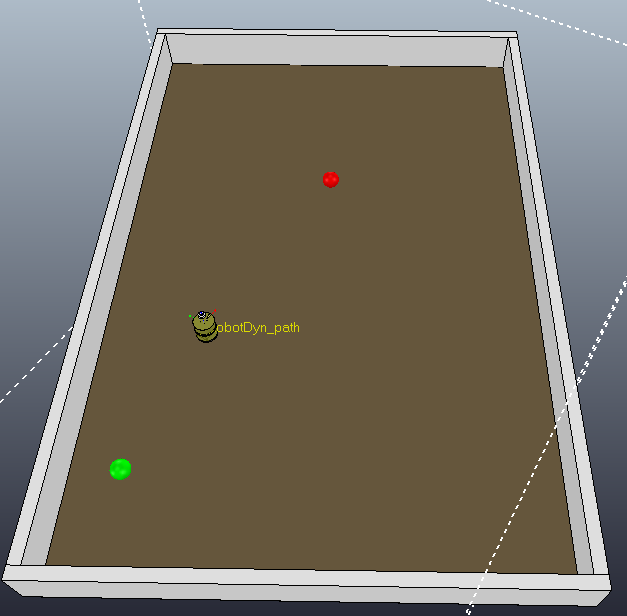
\includegraphics[width=0.7\textwidth]{./img/tar-2-1-arena.png}
  \caption{Target acquisition behavior: Simulation in CoppeliaSim for v = 0 m/s}%
\label{fig:tar-2-1-arena}
\end{figure}
%
\begin{figure}[!hbt]
\centering
    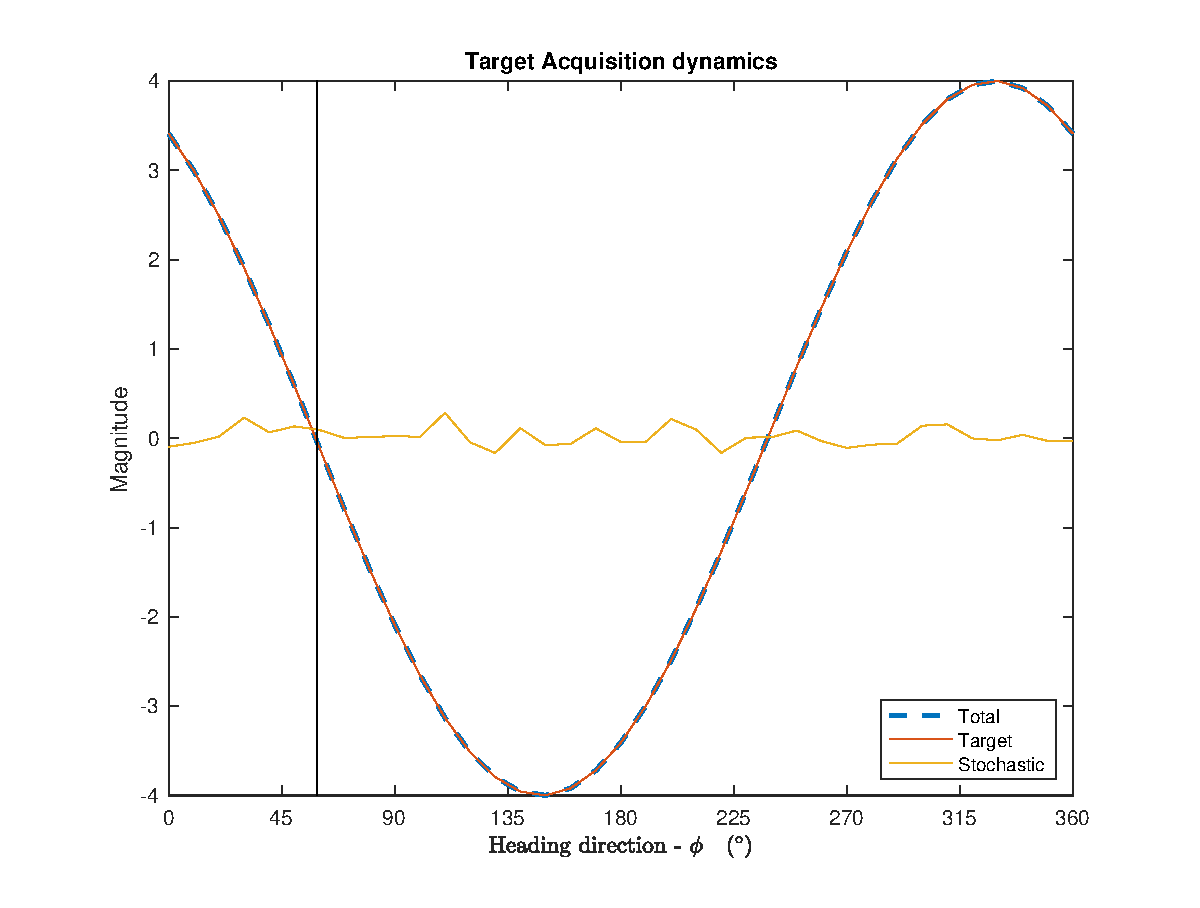
\includegraphics[width=0.6\textwidth]{./img/tar-2-1.eps}
  \caption{Target acquisition behavior: dynamics for v = 0 m/s}%
\label{fig:tar-2-1}
\end{figure}
%
\subsection{Robot moving at constant speed: v = K}%
\label{sec:robot-constant-speed}
After validating the behavior of orientation to the target, it is time to
implement the actual movement to the target by making the linear velocity $v
\neq 0$ m/s. First off, the linear velocity was set to a constant value and the
parameters were tuned, as illustrated in Listing~\ref{lst:program-dyn-tar-2-2},
where the only relevant change in respect to
Section~\ref{sec:robot-initially-at} is the value of the linear velocity.

Fig.~\ref{fig:tar-2-2-arena} depicts the simulation performed for $v = 30$
cm/s. The orientation behavior remains the same, but now the robot moves to the
desired target location (see also Video
\href{run:./videos/tar-2-2.mp4}{./videos/tar-2-2.mp4}), eventually colliding
with it at that speed, as no stop criterion is defined and the linear velocity
is independent from the distance to the target.
Increasing the linear
velocity of the vehicle increases the turning radius, slowing down the
orientation to the target. If the velocity is set too high and the vehicle is
close enough to the arena walls, it may crash against it before even turning (or
while turning).

The dynamics remains identical to the one in
Section~\ref{sec:robot-initially-at} (see Fig.~\ref{fig:tar-2-1}), although
slightly slower due to the increased turning radius for target orientation.
% program_dyn_tar.m (generic)
\lstinputlisting[language=matlab, caption={Target acquisition behavior: Parameter tuning for v = 30 cm/s},label=lst:program-dyn-tar-2-2,
style=custom-matlab]{./listing/program_dyn_tar_2_2.m}%
%
\begin{figure}[!hbt]
\centering
    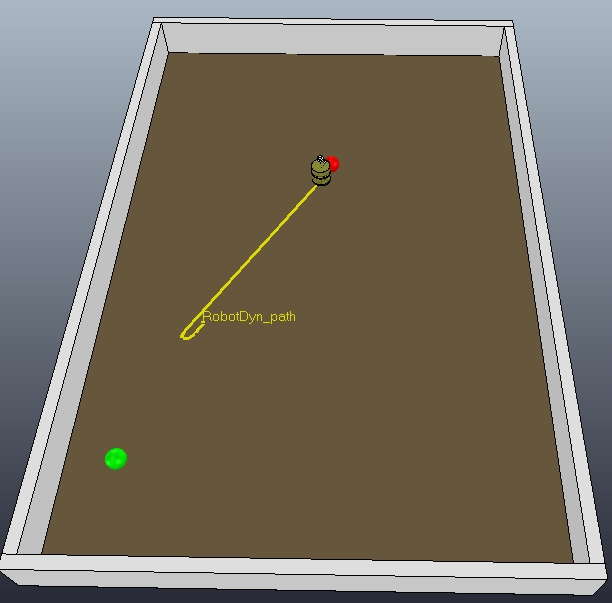
\includegraphics[width=0.7\textwidth]{./img/tar-2-2-arena.png}
  \caption{Target acquisition behavior: Simulation in CoppeliaSim for v = 30 cm/s}%
\label{fig:tar-2-2-arena}
\end{figure}
%
%
\subsection{Robot moving at a velocity defined by a vectorial field}%
\label{sec:robot-moving-vect-field}
Previously, the orientation and movement to the target were validated. However,
the linear velocity of the vehicle was constant and independent of the distance
to the target, which can be problematic especially if the velocity is high or a
stop criterion is undefined.

In this section a linear vectorial field is defined for the linear velocity of
the robot as given by Eq.~(\ref{eq:12}):
%
\begin{equation}
  \label{eq:12}
\frac{dv}{dt} = g_{tar} (v) = \lambda_v (v - v_{des})
\end{equation}
%
where $\gls{v-des}$ is the desired velocity and depends on the distance to the
target.

First, an analytical study of the vectorial field was performed for the
determination of its fixed points and respective stability --- similar to the
one in Section~\ref{sec:analyt-study-tar-nonl} ---  and the phase
portraits and bifurcation diagram were plotted (see
Fig.~\ref{fig:2-3-velocity-vectorial-field}). There is a fixed point at the
desired velocity, i.e., $\gls{v-star} = v_{des}$, which is asymptotically stable (an
attractor) if and only if $\gls{lambda-v} < 0$, yielding the intended
behavior. Additionally, the relaxation time to the attractor is given by
Eq.~(\ref{eq:9}), yielding $\gls{tau-v} = 1 / |\lambda_v| $.
%
\begin{figure}[!hbt]
\centering
    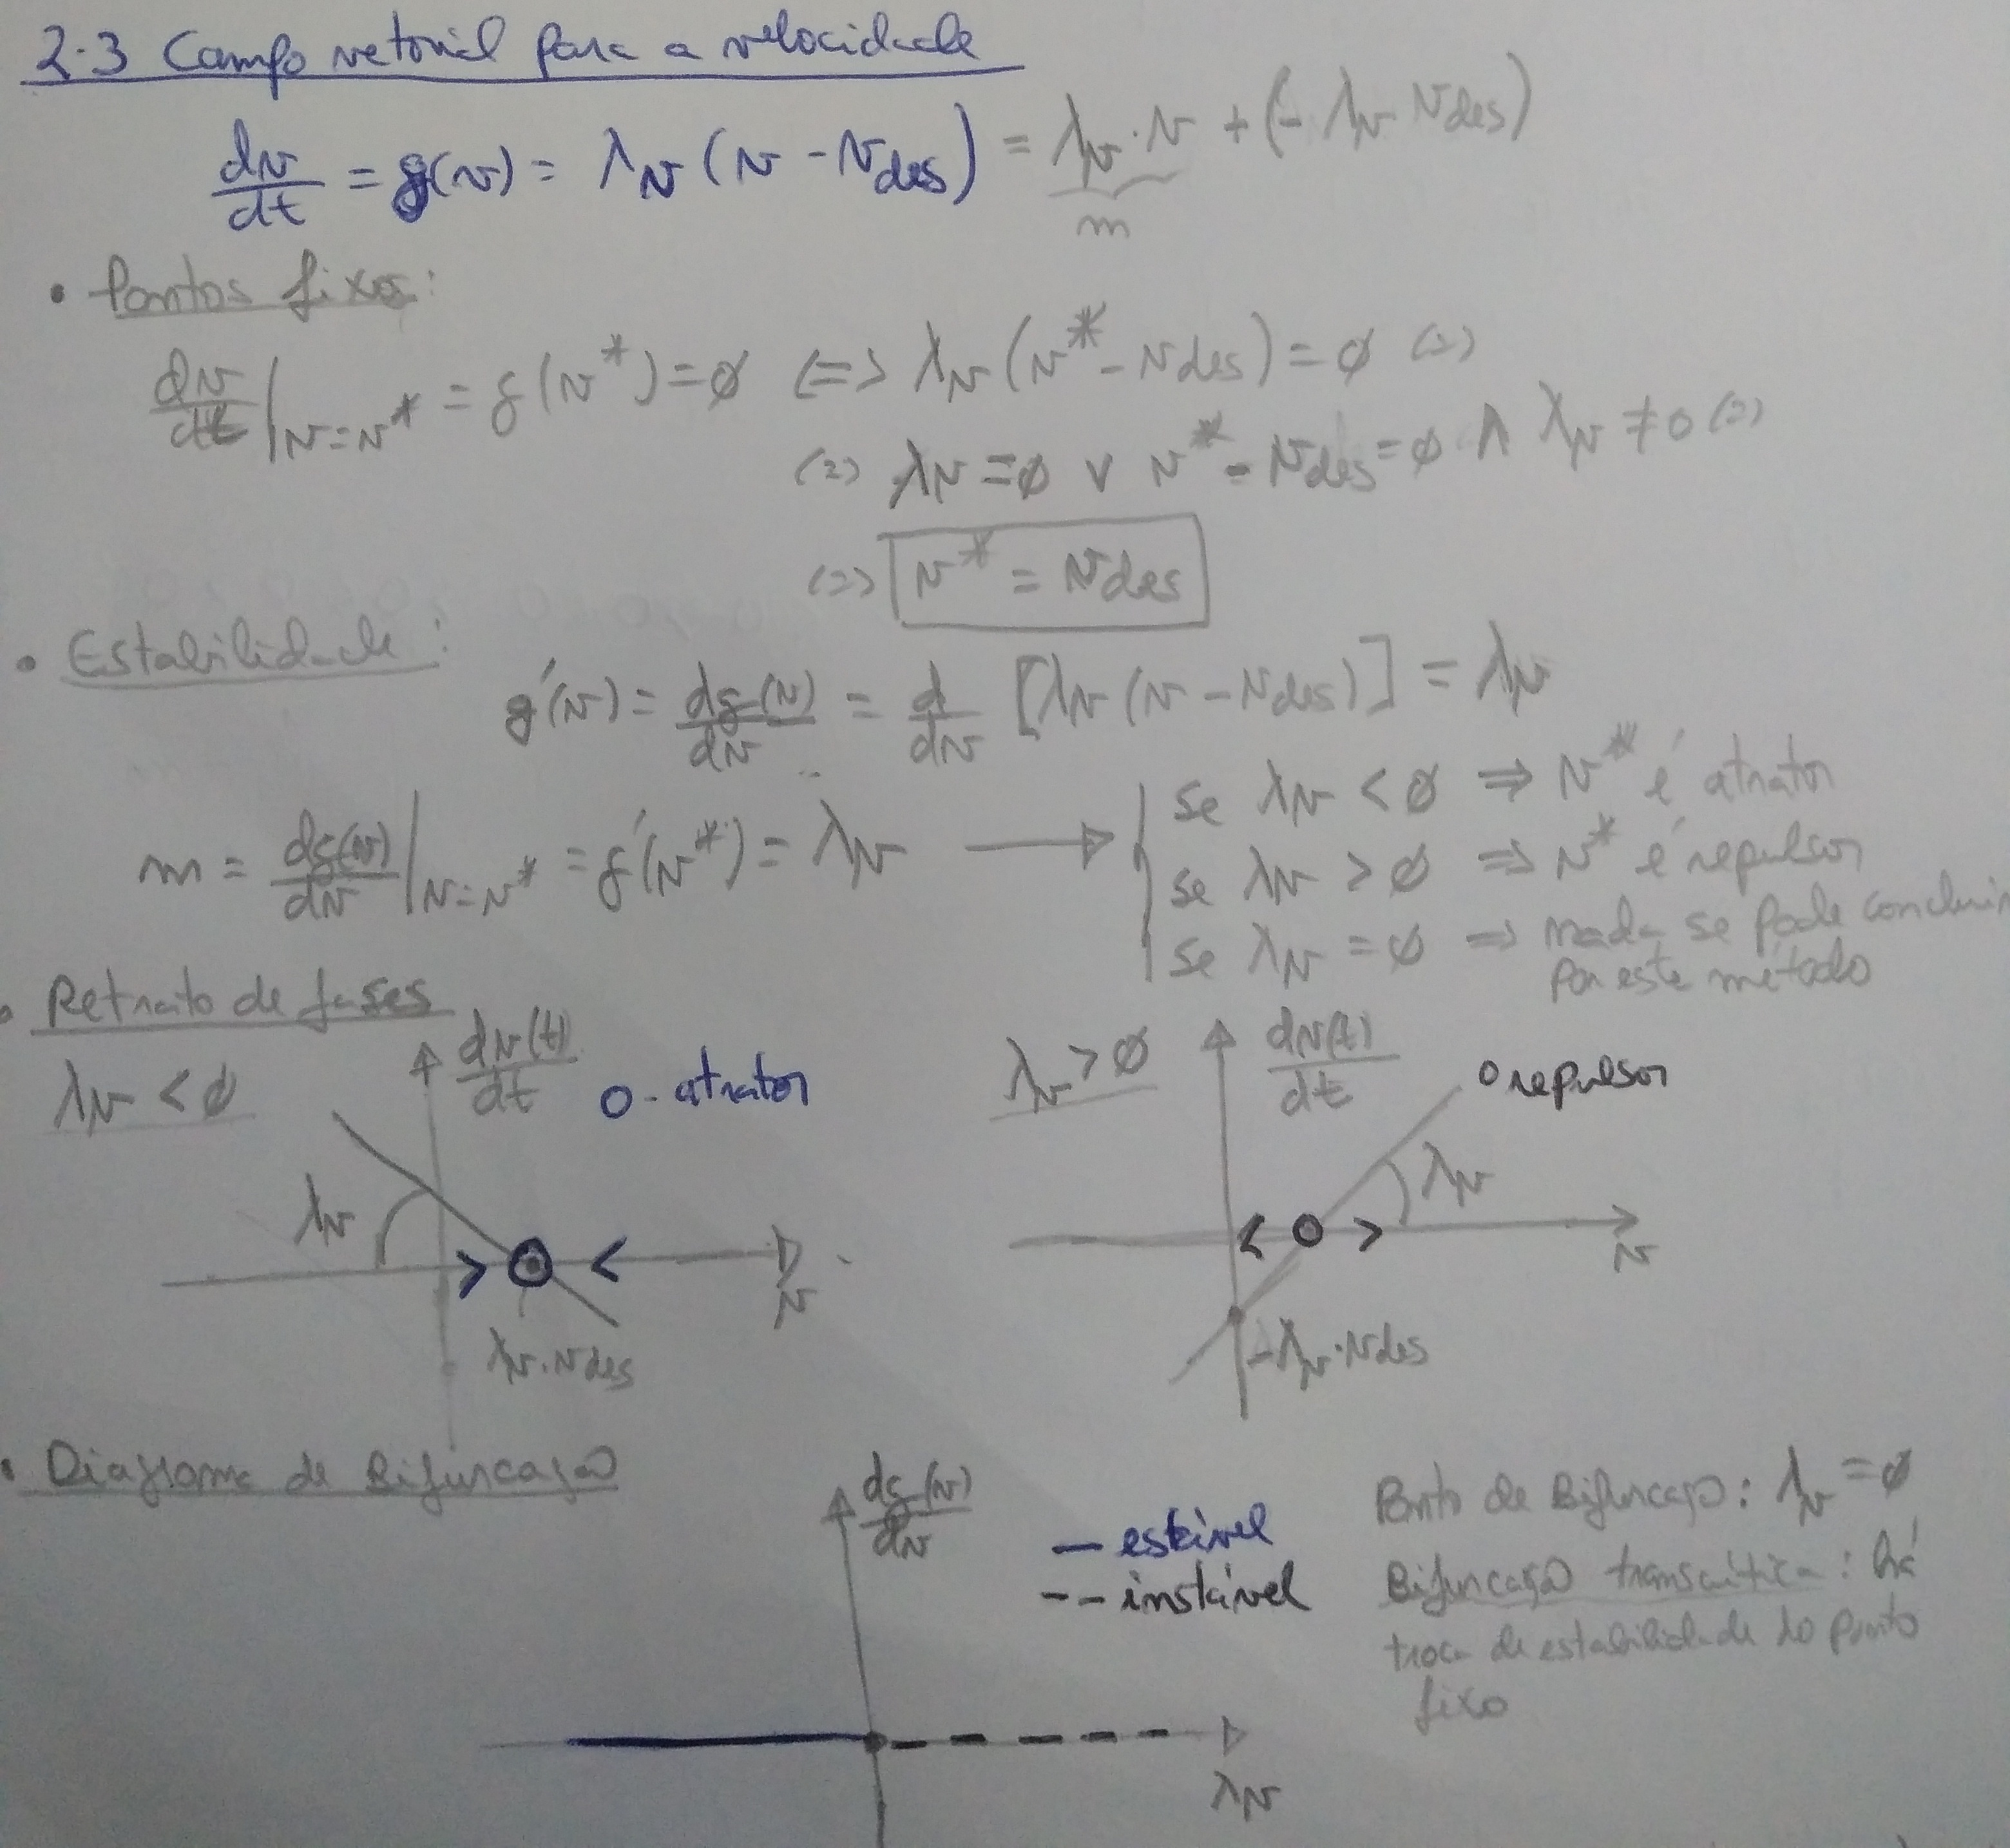
\includegraphics[width=\textwidth]{./img/2-3-velocity-vectorial-field.jpg}
  \caption{Target acquisition behavior: determination of the velocity dynamics}%
\label{fig:2-3-velocity-vectorial-field}
\end{figure}
%

The next step is to convert the first order differential equation into a
algebraic recursive equation in a discrete form (Eq.~(\ref{eq:13})):
\begin{equation}
  \label{eq:13}
v(t + \Delta t) = v(t) + \Delta t g_{tar}(v), \qquad v(t_0) = v_0
\end{equation}

Noting that $g_{tar}(v) = d v(t)/dt = a(t)$, one can write:
\begin{equation}
  \label{eq:15}
v(t + \Delta t) = v(t) + \Delta t a(t), \qquad v(t_0) = v_0
\end{equation}
which represents the equation of the uniformly varied rectilinear motion, with
$\gls{a}(t)$ being the acceleration of the robot. If $a(t) > 0$ the motion is
accelerated and reciprocally if $a(t) < 0$ the motion is retarded. Thus, one can
analyse the sign of $a(t)$ to understand the motion of the robot. Recalling that
$\lambda_v < 0$:
%
\begin{equation}
  \label{eq:16}
a(t) = g(v) = \left\{
\begin{array}{ll}
      > 0 , & (v - v_{des}) \leq 0 \\
      < 0 , & (v - v_{des}) > 0 \\
\end{array} 
\right. \leftrightarrow a(t) = g(v) = \left\{
\begin{array}{ll}
      > 0 , & v \leq v_{des} \\
      < 0 , & v > v_{des} \\
\end{array} 
\right. 
\end{equation}
%
the motion will be accelerated if $v \leq v_{des}$ --- which represents the
initial condition, ramping from rest to the desired velocity --- and retarded if
$v > v_{des}$ --- the inertia and delayed actuation (as a consequence of the
timestep) may lead to excessive velocity. On the other hand, the linear velocity
should converge to a constant value in the vicinity of the desired velocity
($a(t) = 0 \rightarrow v(t + \Delta t) = v(t)$).
%\begin{equation*}
%\frac{\Delta v}{\Delta t} = \lambda_v (v - v_{des}) \quad \leftrightarrow \quad v(t + \Delta t) - v(t) = \Delta t \lambda_v (v(t) - v_{des})
%\end{equation*}
%Rearraging the terms, the algebraic recursive equation for the linear velocity
%dynamic system becomes:
%\begin{equation}
%  \label{eq:13}
%v(t + \Delta t) = v(t) ( 1 + \Delta t \lambda_v) +  \Delta t \lambda_v v_{des}
%\end{equation}

With this in mind, one must determine the desired velocity as a function of the
distance to the target. Ideally, one desires a steady increase of velocity with
the distance and a plateau for the maximum velocity, which can be expressed as:
%
\begin{equation}
  \label{eq:14}
  v_{des} (d) = v_{max} - v_{max} e^{- \frac{d}{\tau_{vdes}}} \quad
  \leftrightarrow \quad
  v_{des} (d) = v_{max} \Big (1 - e^{- \frac{d}{\tau_{vdes}}} \Big )
\end{equation}
where $\gls{vmax}$ is the maximum velocity (cm/s) and $\gls{tau-vdes}$ is the time
constant for the desired velocity increase.

Fig.~\ref{fig:linear-vel-funcs-comparison} illustrates a comparison of
functions for the desired velocity as a function of distance, $v_{des}(d)$. The
maximum velocity considered was 80 cm/s.
The dashed line corresponds to the linear function $v_{des}(d) = \gls{kv} d$, with $k
= 1$, which acts as a guideline, although it could also be used, provided the
$v_{max}$ threshold was defined. For $\tau_{vdes} \leq 20$ s, the robot would hit the
target fast, which can be problematic due to path corners and
inertia; for $\tau_{vdes} \ge 75$ s it can be
slow. A tradeoff between velocity and path smoothness must be considered, as
detailed further ahead.     
%
\begin{figure}[!hbt]
\centering
    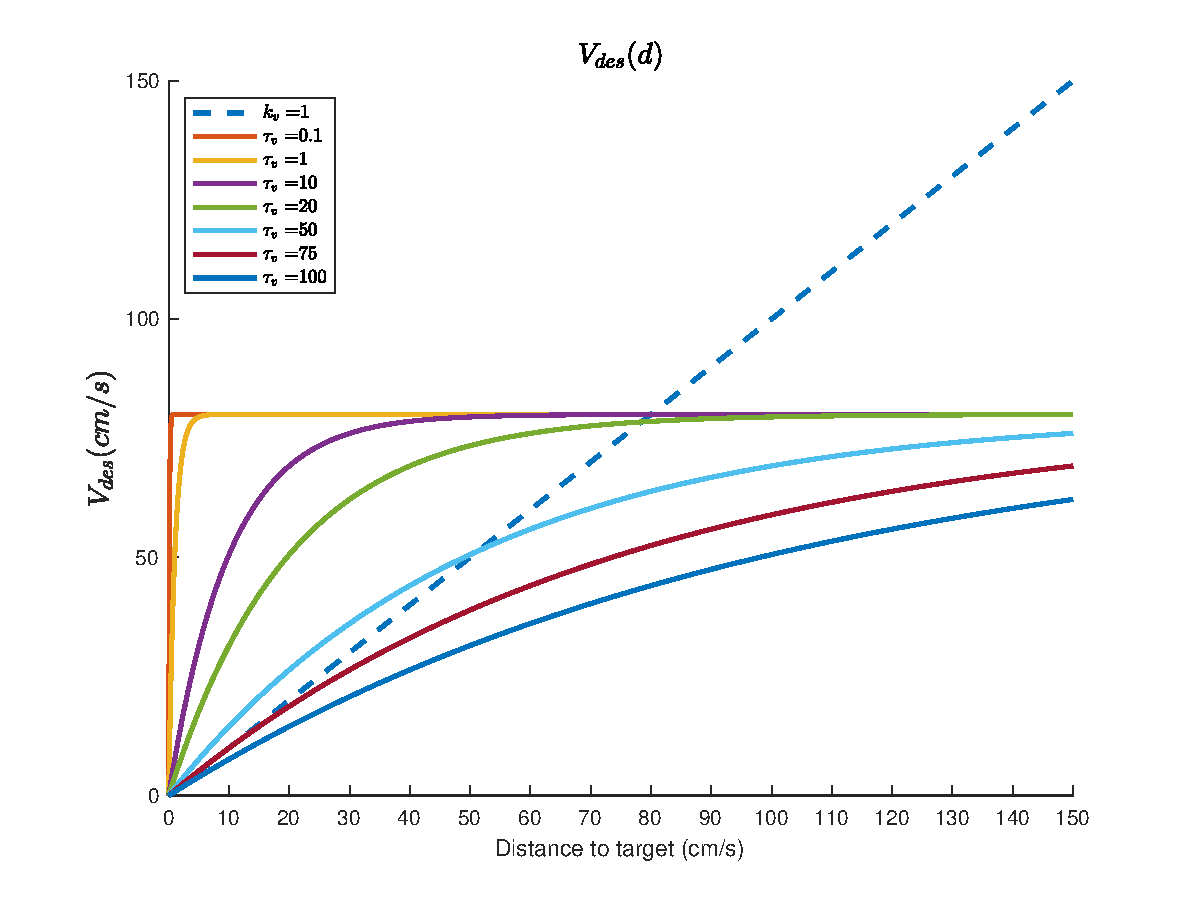
\includegraphics[width=0.7\textwidth]{./img/linear-vel-funcs-comparison.eps}
  \caption{Target acquisition behavior: comparison of functions $v_{des} (d)$}%
\label{fig:linear-vel-funcs-comparison}
\end{figure}

Lastly, the distance to the target, $gls{d}$, must be determined. It can be seen from
Fig.~\ref{fig:fig1} the distance to the target is given by the
euclidean distance in the cartesian plane, i.e.:
\begin{equation}
  \label{eq:17}
  d = \sqrt{ (x_{robot} - x_{tar})^2 + (y_{robot} - y_{tar})^2}
\end{equation}

However, the coordinates of the robot and the target are of their centers of
mass, which indicates an horizontal shift of magnitude $\gls{d-min}$ (minimum
distance) should be performed to the exponential functions illustrated in
Fig.~\ref{fig:linear-vel-funcs-comparison}, yielding:
\begin{equation}
  \label{eq:18} 
v_{des} = \left\{
\begin{array}{ll}
 v_{max} \Big (1 - e^{- \frac{d - d_{min}}{\tau_{vdes}}} \Big ), & d \geq d_{min} \\
      0 , & d < d_{min} \\
\end{array} 
\right.
%\quad (\mathrm{exponential})
\end{equation}
as illustrated in Fig.~\ref{fig:linear-vel-funcs-comparison-shift}.
The minimum distance is calculated as $d_{min} = R_{robot} + R_{tar}$, where
$\gls{Rrobot}$ and $\gls{Rtar}$ are the radius of the robot's base (22.5 cm) and
target (20 cm), respectively, yielding $d_{min} = 42.5$ cm.
%
\begin{figure}[!hbt]
\centering
    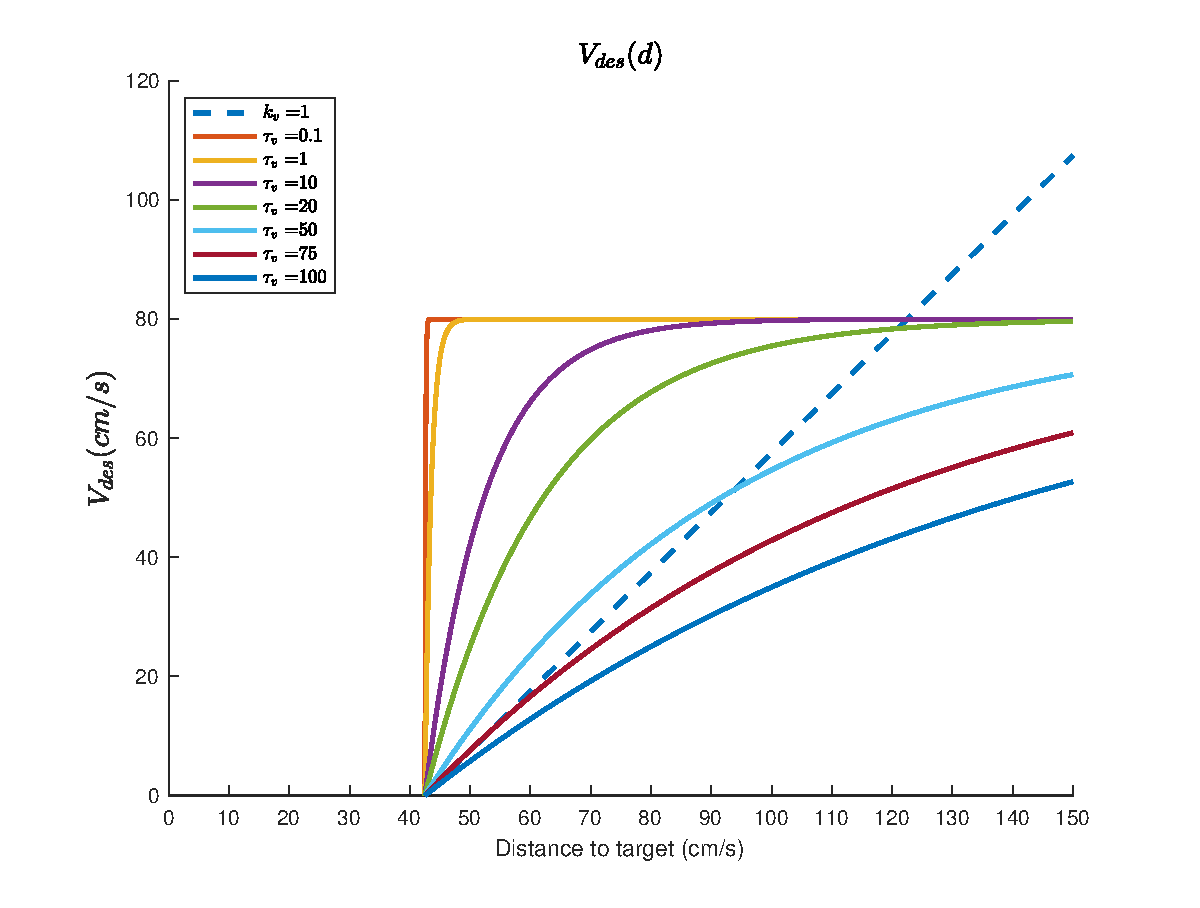
\includegraphics[width=0.7\textwidth]{./img/linear-vel-funcs-comparison-shift.eps}
  \caption{Target acquisition behavior: comparison of functions $v_{des} (d)$
    (with minimum distance shift)}%
\label{fig:linear-vel-funcs-comparison-shift}
\end{figure}
%
%where $k_v$ is the velocity gain with the distance to the target, with $k_v > 0$
%for velocity increase with the distance.

%For this purpose the exponential was chosen has indicated in
%Eq.~(\ref{eq:14}):
%\begin{equation}
%  \label{eq:14}
%  v_{des} (d) = v_{0} \exp(\beta_v d)
%\end{equation}
%where $v_0$ is the velocity near the target (minimum) and $\beta_v$ defines the
%growing rate of the desired velocity as the distance increases.
%

The vector field for linear velocity was implemented (see
(Listing~\ref{lst:program-dyn-tar-vel})) and the parameters were tuned. 
The desired behavior for the robot is faster orientation to target, i.e.,
heading direction dynamics takes precedence over velocity
dynamics. Additionally, the $v_{des}(d)$ must have a slower influence on the
velocity dynamics (smoother curve) to avoid steep accelerations.
Thus, the hierarchy of time constants for the system is: $\tau_{tar} \ll \tau_{v}
\ll \tau_{vdes}$.
% program_dyn_tar.m (generic)
\lstinputlisting[language=matlab, firstline=1,lastline=43,
caption={Implementation of target acquisition behavior with dynamic field for
  linear velocity},label=lst:program-dyn-tar-vel,
style=custom-matlab]{./listing/program_dyn_tar_vel.m}%

The heading direction and velocity dynamics were also plotted, alongside with
$v_{des}(d)$ (see Listing~\ref{lst:program-dyn-tar-vel2}) to aid the behavior analysis.
\lstinputlisting[language=matlab, firstline=89,lastline=141,
caption={Implementation of target acquisition behavior with dynamic field for
  linear velocity},label=lst:program-dyn-tar-vel2,
style=custom-matlab]{./listing/program_dyn_tar_vel.m}%

Fig.~\ref{fig:tar-linear-vel-arena} illustrates the simulation in CoppeliaSim
for the linear velocity dynamics implementation (see also Video
\href{run:./videos/tar-2-3-linear-vel.mp4}{./videos/tar-2-3-linear-vel.mp4}). It can be seen that the robot
successfully moves to target, remaining at a minimum distance. The turning
radius is small, as the heading dynamics has a stronger effect over the robot
than the velocity dynamics. Additionally, during this simulation it was noted
the robot accelerates in the beginning to $1/3$ of the overall distance
$g_{tar}(v) > 0$ and decelerates until it reaches the target (within the minimum
distance). The final state of the simulation is illustrated for $v_{des}(d)$ and
$g_{tar}(v)$ in Figs.~\ref{fig:tar-2-3-vdes} and~\ref{fig:tar-2-3-g-v}. It can
be seen that the desired velocity reaches $0$ m/s and the corresponding dynamics
$g_{tar}(v)$ is near the attractor in deceleration, as expected.
%
\begin{figure}[!hbt]
\centering
    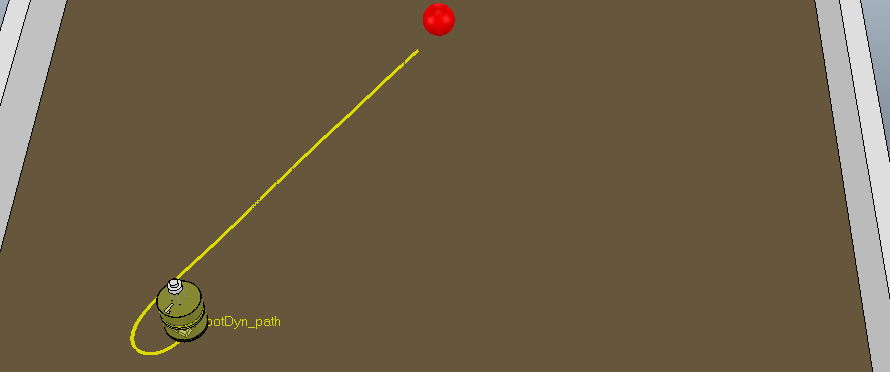
\includegraphics[width=0.7\textwidth]{./img/tar-2-3-arena.png}
  \caption{Target acquisition behavior: velocity dynamics simulation in CoppeliaSim}%
\label{fig:tar-linear-vel-arena}
\end{figure}
%
\begin{figure}[!hbt]
\centering
    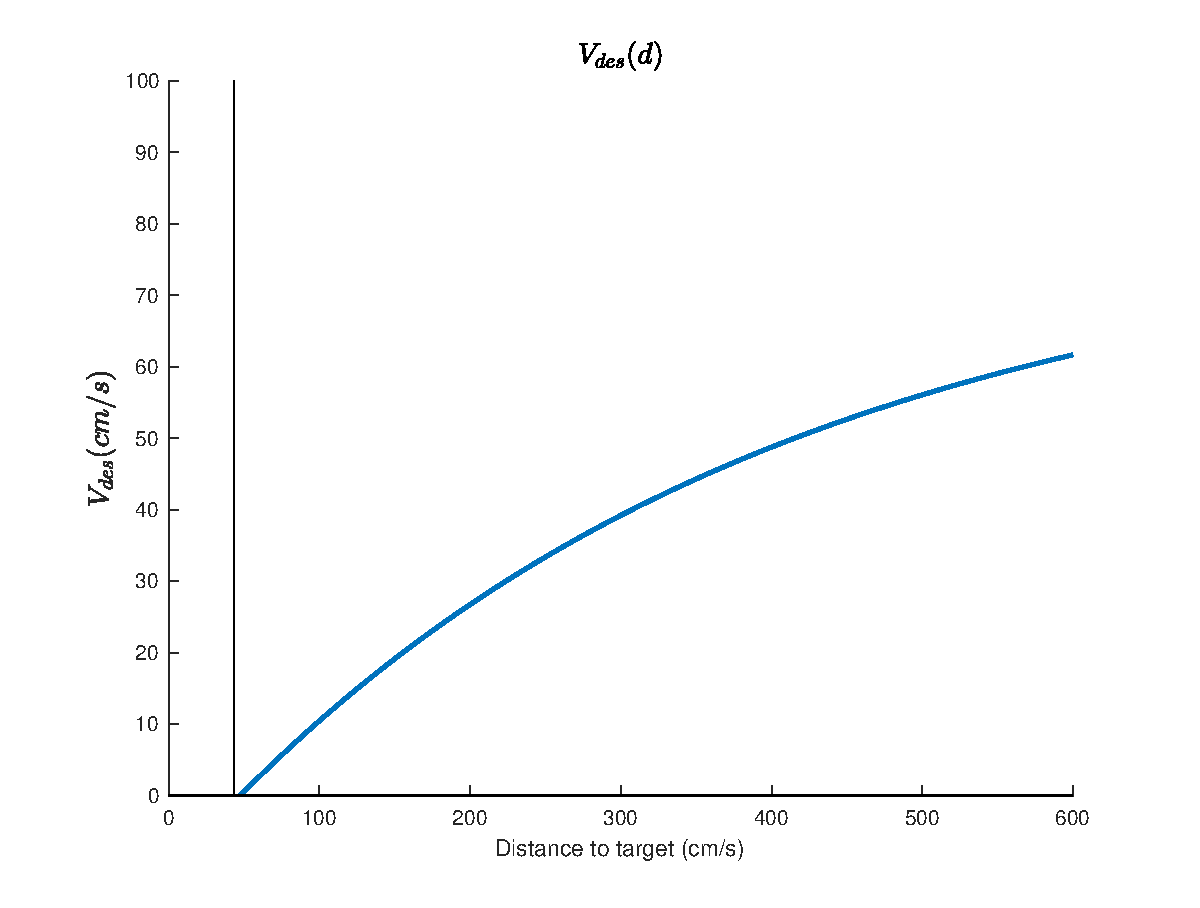
\includegraphics[width=0.7\textwidth]{./img/2-3-vdes.eps}
    \caption{Target acquisition behavior: velocity dynamics simulation ---
      $v_{des} (d)$}%
\label{fig:tar-2-3-vdes}
\end{figure}
%
\begin{figure}[!hbt]
\centering
    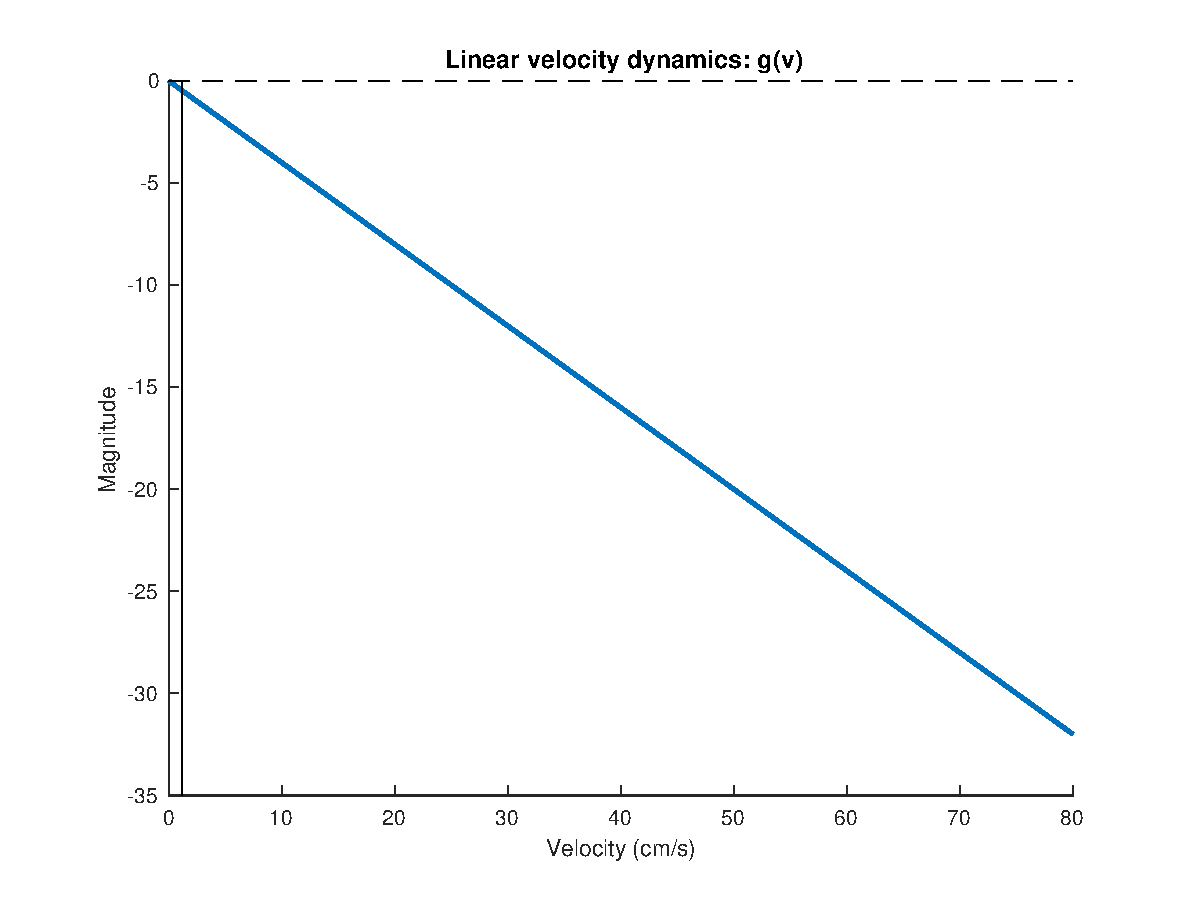
\includegraphics[width=0.7\textwidth]{./img/2-3-g-v.eps}
  \caption{Target acquisition behavior: velocity dynamics simulation ---
    $g_{tar} (v)$}%
\label{fig:tar-2-3-g-v}
\end{figure}
%
\section{Discussion}%
\label{sec:discussion-tar-nonl}
As aforementioned (See Section~\ref{sec:robot-moving-vect-field}), the robot
moves to the target with variable velocity: it accelerates in the beginning to
$1/3$ of the overall distance $g_{tar}(v) > 0$ and decelerates until it reaches
the target (within the minimum distance).
The heading direction dynamics takes precedence
over the velocity dynamics to allow smooth navigation to the target: the robot
orientates itself faster to the target than it actually moves. 
Additionally, the $v_{des}(d)$ has a slower influence on the
velocity dynamics (smoother curve) to avoid steep accelerations.
Thus, the hierarchy of time constants for the system is: $\tau_{tar} \ll \tau_{v}
\ll \tau_{vdes}$.
The heading direction dynamics is illustrated in Fig.~\ref{fig:tar-2-1} and
in Figs.~\ref{fig:tar-2-3-vdes} and~\ref{fig:tar-2-3-g-v} can
be seen that the desired velocity reaches $0$ m/s and the corresponding dynamics
$g_{tar}(v)$ is near the attractor in deceleration, as expected.

\section{Linear dynamic system for heading direction}%
\label{sec:line-dynam-syst}
In this section a linear dynamic system for the heading direction was analyzed:
\begin{equation}
  \label{eq:19}
  \frac{d \phi}{dt} = f_{tar}(\phi) = - \lambda_{tar}(\phi - \psi_{tar})
\end{equation}

The fixed points and its stability was determined. The phase portraits
were plotted and compared to the nonlinear counterpart. Next, the linear dynamic
system was implemented and simulated, observing some differences of the
navigation paths due to higher angular velocity range. Lastly, the linear and
nonlinear dynamic system were compared, determing the best suited for the task
of target acquisition behavior of the robot.
%
\subsection{Fixed points}%
\label{sec:fixed-points-linear-phi}
The fixed points of the linear dynamic system can be determined as its constant
solutions, i.e.:
\begin{equation}
  \label{eq:20}
\begin{array}{ll}
  \left. \frac{d \phi}{dt}\right|_{\phi = \phi^*} = f_{tar}(\phi^*) = 0 \quad 
  \leftrightarrow \quad - \lambda_{tar} (\phi^* - \psi_{tar}) = 0\\
      \quad \leftrightarrow \quad 
  (\lambda_{tar} = 0 \vee \phi^* - \psi_{tar} = 0) \wedge \lambda_{tar} \ne 0
  \quad \leftrightarrow \quad \boxed{\phi^* = \psi_{tar}} \\
\end{array} 
\end{equation}
%
There is one fixed point at $\phi^* = \psi_{tar}$.
%
\subsection{Stability}%
\label{sec:stability-linear-phi}
The determination of the stability of fixed points is useful to understand its
qualitative behavior. It can be determined analytically using Eq.~(\ref{eq:21}):
%
\begin{equation}
  \label{eq:21}
  m = \left. \frac{d f_{tar}(\phi)}{d \phi}\right|_{\phi = \phi^*} = f'_{tar}(\phi^*)
  \quad \leftrightarrow \quad  \boxed{m = - \lambda_{tar}}\\
\end{equation}

Analyzing the possible cases for the slope at the fixed points, it can be
observed that:
\begin{equation}
  \label{eq:22}
  m = \left\{
\begin{array}{ll}
      < 0 , & \lambda_{tar} > 0 \quad \rightarrow \quad \mathrm{attractor} \\
      > 0 , & \lambda_{tar} < 0 \quad \rightarrow \quad \mathrm{repeller} \\
      = 0 , & \lambda_{tar} = 0 \quad \rightarrow \quad \mathrm{inconclusive} \\
\end{array} 
\right. 
\end{equation}
The desired heading direction dynamics requires that an attractor is placed in
the target direction, i.e. $\phi^* = \psi_{tar}$ is an attractor, thus
$\lambda_{tar} > 0$. The relaxation time for the attractor is given by:
\begin{equation}
  \label{eq:23}
 \tau_{tar} = \frac{1}{| f'_{tar}(\phi^*) |} \quad \leftrightarrow \quad \boxed{\tau_{tar} = \frac{1}{\lambda_{tar}}}
\end{equation}
%
\subsection{Phase portraits}%
\label{sec:phase-portraits-1}
Fig.~\ref{fig:tar-4-3} illustrates the different phase portraits for the linear
dynamic system of the heading direction $\phi \in [0, 2 \pi[$ (circular phase
space). Comparing the phase portraits between linear and nonlinear dynamic
systems, respectively Figs.~\ref{fig:tar-4-3} and~\ref{fig:1-3-phase-portraits},
it can be observed that the former has one fixed point only --- 
attractor or repeller depending on the value of the parameter $\lambda_{tar}$,
but not both on the same phase portrait --- while the latter has two fixed
points --- one attractor and one repeller on each phase portrait.
%
\begin{figure}[!hbt]
\centering
    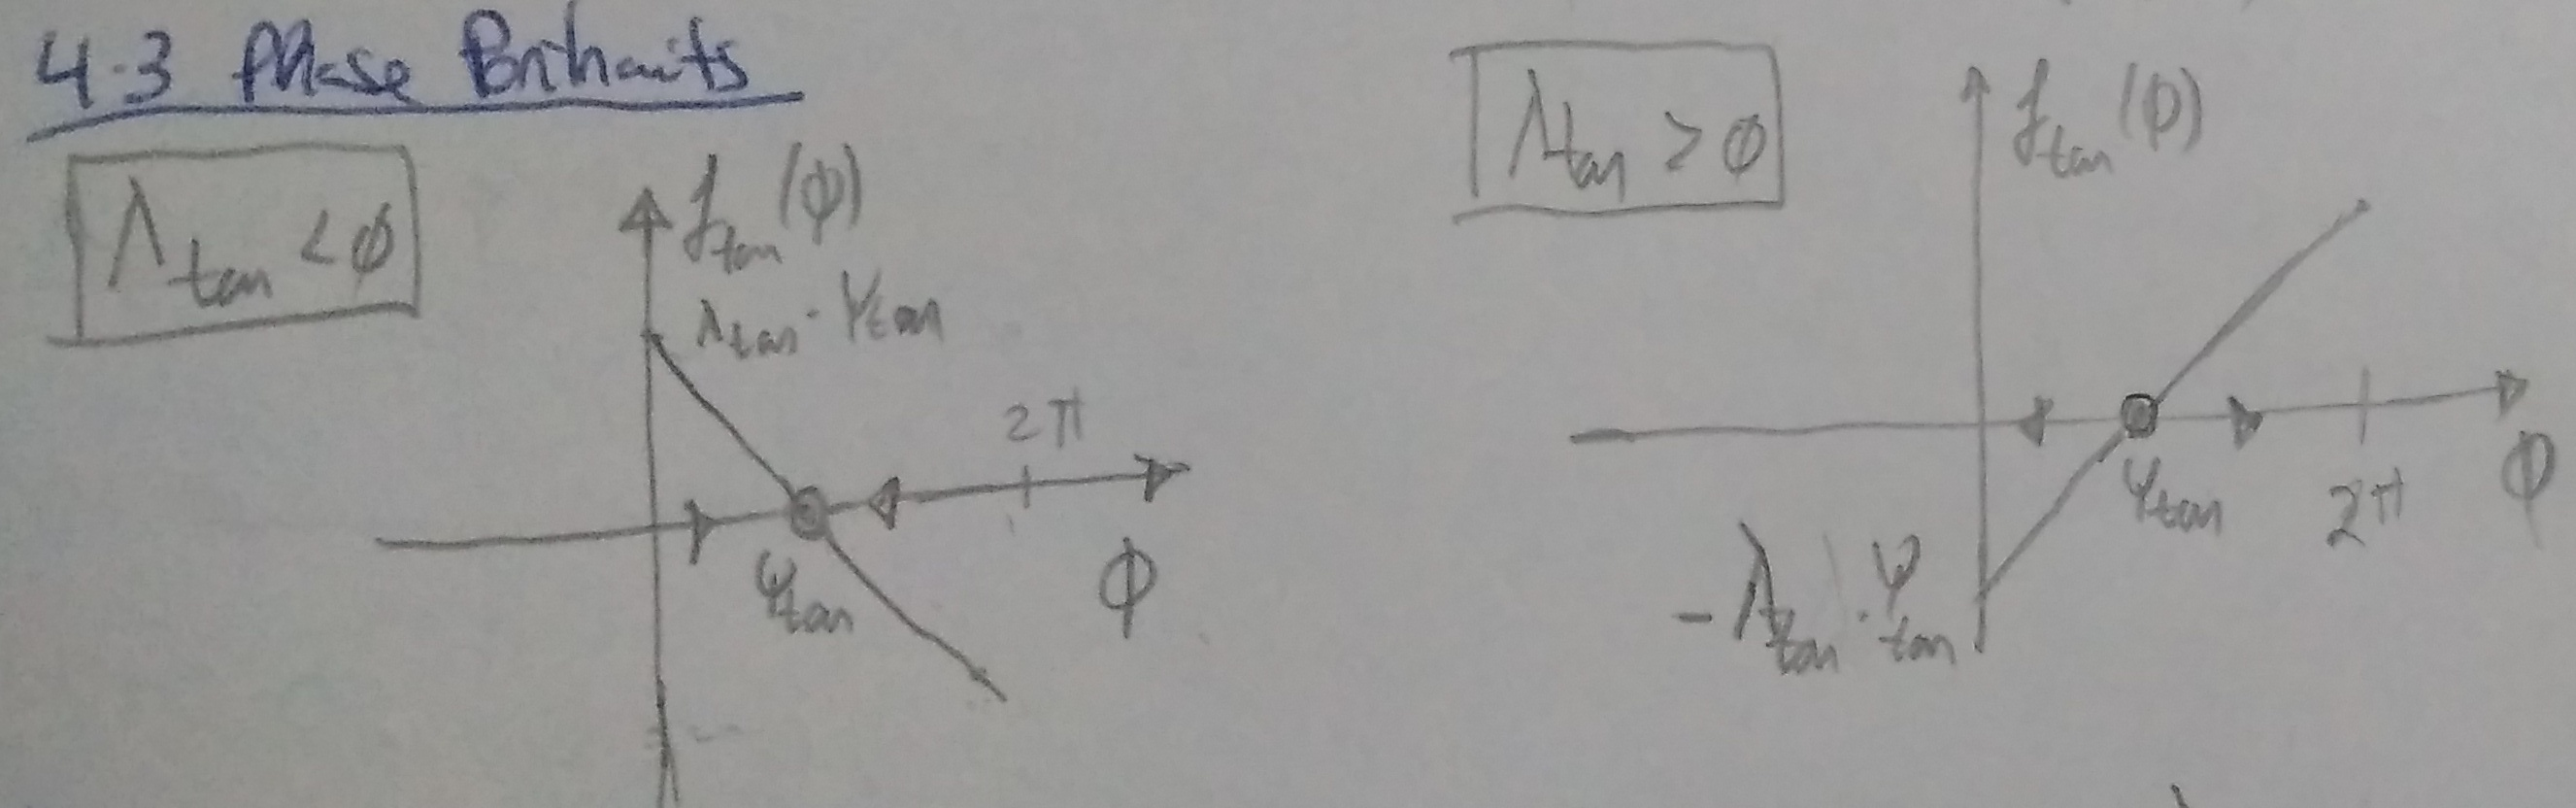
\includegraphics[width=0.8\textwidth]{./img/tar-4-3.jpg}
  \caption{Target acquisition behavior: linear dynamic system for heading
    direction --- phase portraits}%
\label{fig:tar-4-3}
\end{figure}
%
%
\subsection{Implementation}%
\label{sec:implementation-linear-phi}
The implementation of the linear dynamic system for the heading direction was
performed considering also the linear dynamic system for linear velocity, i.e.,
modifying the implementation from Section~\ref{sec:robot-moving-vect-field} with
respect to the heading direction dynamics as follows: 
%
\begin{lstlisting}[language=matlab, caption={Implementation of linear dynamic
system for heading direction},label=lst:program-dyn-tar-linear-phi,
style=custom-matlab]%

% dynamic system
ftar = -lambda_tar * (phirobot - psi_tar);
% plot
ftar_plot = -lambda_tar * (phi_plot - psi_tar);

\end{lstlisting}

The same considerations, in respect to the nonlinear dynamic system, needed to
be applied, namely $\Delta t \ll \tau_{tar}$.

\subsection{Discussion}%
\label{sec:discussion-linear-phi}
Fig.~\ref{fig:tar-4-4-arena} illustrates the simulation of the linear dynamic
system for heading direction implemented (see also \href{run:./videos/tar-4-4.mp4}{./videos/tar-4-4.mp4}), and Fig.~\ref{fig:tar-4-4} contains
the final state of the dynamics. Comparing Fig.~\ref{fig:tar-4-4-arena} with
Fig.~\ref{fig:tar-linear-vel-arena}, respectively the simulation of linear and
nonlinear dynamics, it can be observed the smaller curvature radius
corresponding to the initial orientation to the target for the former. This is
due to the higher magnitude of the attractive force-let (linear) (higher angular
velocity) for linear dynamics, as compared to
the repulsive and attractive force-lets (sinusoidal) for nonlinear
dynamics. The nonlinear dynamic system is better suited for target acquisition
behavior of the robot, as it provides smoother paths --- narrower angular
velocity range.
%
\begin{figure}[!hbt]
\centering
    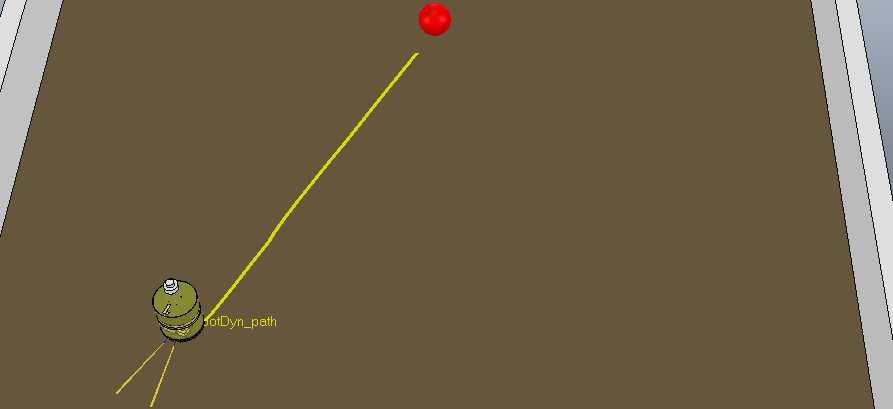
\includegraphics[width=0.65\textwidth]{./img/tar-4-4-arena.png}
  \caption{Target acquisition behavior: linear dynamic system for heading
    direction --- simulation}%
\label{fig:tar-4-4-arena}
\end{figure}
%
\begin{figure}[!hbt]
\centering
    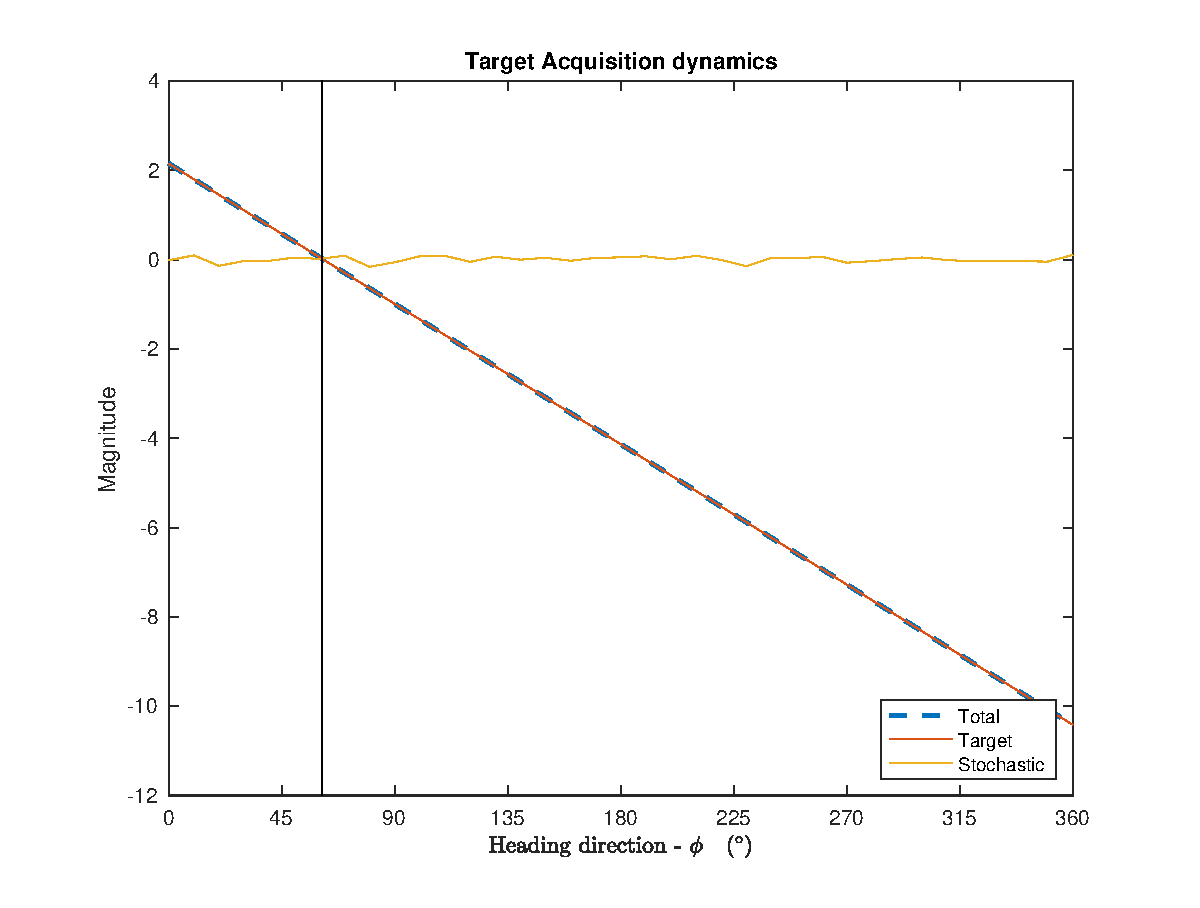
\includegraphics[width=0.65\textwidth]{./img/tar-4-4.eps}
  \caption{Target acquisition behavior: linear dynamic system for heading
    direction --- dynamics (final state)}%
\label{fig:tar-4-4}
\end{figure}
%
%
%
%%% Local Variables:
%%% mode: latex
%%% TeX-master: "../../dissertation"
%%% End:

  \setcounter{table}{0}
  \setcounter{figure}{0}
%  
  \chapter{Obstacle Avoidance}%
\label{ch:obstacle-avoidance}
While moving to a target, a robot must also avoid obstacles that may appear ---
obstacle avoidance. To avoid obstacles, the robot must firstly detect them, in
this case, using infrared radiation sensors mounted in a circular support which
is centered in respect to the rotation axis of the robot
(Fig.~\ref{fig:fig2-obs}). Each sensor is mounted in a fixed direction
$\gls{theta-i}$ in respect to frontal direction of the robot, i.e., the heading
direction. Thus, each sensor points into a direction $\gls{psi-obs-i} = \phi + \theta_i$,
in respect to the external reference axis~\cite{bicho2000dynamic}.
%
\begin{figure}[!hbt]
\centering
    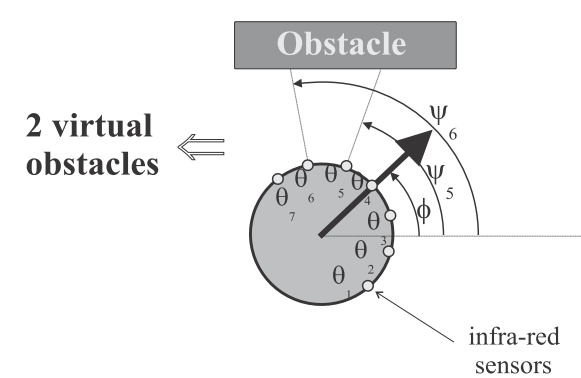
\includegraphics[width=0.55\textwidth]{./img/fig2-obstacles.png}
  \caption{Obstacle avoidance behavior: sensor placement}%
\label{fig:fig2-obs}
\end{figure}

The strategy adopted consists in assuming that each sensor $i$ specifies a
virtual obstacle in the direction $\psi_{obs,i}$ if an obstruction is detected
in that direction. Each virtual obstacle is modelled by a repulsive force
centered in the direction the respective sensor points out:
\begin{equation}
  \label{eq:24}
  f_{obs,i}(\phi) = \lambda_{obs,i} (\phi -\psi_{obs,i}) \exp \Big(-\frac{(\phi - \psi_{obs,i})^2}{2 \sigma_i ^2} \Big)
  = \lambda_{obs,i} (- \theta_i) \exp \Big(-\frac{(- \theta_i)^2}{2 \sigma_i ^2} \Big)
\end{equation}
It must be pointed out that the only diference $\phi - \psi_{obs,i} = - \theta_i$,
which is fixed and known, goes into the heading direction dynamics, thus
yielding the calibration of the system in respect to the external reference axis
irrelevant.

The strength of the repulsion, $\gls{lambda-obs-i}$, from the virtual obstacle at
direction $\gls{psi-obs-i}$, is a decreasing function of the sensed distance, $\gls{d-i}$ ---
high for small distances and low for high distances and null for $d_i \ge
d_{max}$ (sensor range maximum) --- which can be exponential:
\begin{equation}
  \label{eq:25}
  \lambda_{obs,i} = \beta_1 \exp \Big( -\frac{d_i}{\beta_2} \Big)
\end{equation}
where $\gls{beta1}$ determines the maximum strenght of repulsion and $\gls{beta2}$ is
the decay rate of the repulsion force with the distance increase.

The angular range over which the force-let exerts its repulsive effect, 
$\gls{sigma-i}$ is given by:
\begin{equation}
  \label{eq:26}
  \sigma_{i} = \arctan \Bigg( \tan \Big(\frac{\Delta \theta}{2} \Big ) + 
  \frac{R_{robot}}{R_{robot} + d_i}\Bigg)
\end{equation}
where $\gls{delta-theta}$ is the angular distance between adjacent sensors (sensor
sector), $R_{robot}$ is the radius of the robot, and $d_i$ is the distance
estimated by the sensor $i$.

The contributions from all the sensors are summed, thus, yielding the overall
obstacle avoidance dynamics as follows:
\begin{equation}
  \label{eq:27}
 \frac{d \phi}{dt} = \gls{F-obs}(\phi) = f_{obs}(\phi) + f_{stoch}
%\quad N = nr of sensors
\end{equation}
where $N$ is the number of sensors, in this case, $\gls{N} = 11$, $\gls{f-obs}$ is the
total repulsion force due to all obstacles contributions (Eq.~(\ref{eq:35})),
and $f_{stoch}$ is
the stochastic force given by Eq.~(\ref{eq:6}).
\begin{equation}
  \label{eq:35}
  f_{obs} (\phi) = \sum_{i = 1}^N \gls{f-obs-i}(\phi) 
\end{equation}

\section{Analytical study}%
\label{sec:analytical-study-obs}
In this section the analytical study of the overall obstacle avoidance dynamics
(Eq.~(\ref{eq:27})) is performed. The fixed points are determined and its
stability assessed. The phase portraits and bifurcation diagram are
plotted. Lastly, the range of admissible values for the parameter $\beta_1$ and
the repulsion time constant are computed.

\subsection{Fixed points}%
\label{sec:fixed-points-obs}
The fixed points for the dynamic system given by Eq.~(\ref{eq:27}) are computed,
considering that only one obstruction is detected, i.e.:
\begin{equation}
  \label{eq:28}
 \frac{d \phi}{dt} = F_{obs}(\phi) = f_{obs,1}(\phi)
\end{equation}
%
The fixed points are the constant solutions of the dynamic system, i.e.:
\begin{equation}
  \label{eq:29}
\begin{array}{ll}
  \left. \frac{d \phi}{dt}\right|_{\phi = \phi^*} = f_{obs, 1}(\phi^*) = 0 
\quad \leftrightarrow \quad 
  \lambda_{obs,1} (\phi^* -\psi_{obs,1}) \exp \Big(-\frac{(\phi^* - \psi_{obs,1})^2}{2 \sigma_i ^2} \Big) = 0 
\quad \leftrightarrow \quad 
\\ 
\quad \leftrightarrow \quad (\lambda_{obs,1} = 0 \vee \phi^* - \psi_{obs,1} = 0 \vee  \exp \Big(-\frac{(\phi^* - \psi_{obs,1})^2}{2 \sigma_i ^2} \Big) = 0) \wedge \lambda_{obs,i} \ne 0
\\ 
\quad \leftrightarrow \quad 
\boxed{\phi^* = \psi_{obs,1}}
\end{array}
\end{equation}
There is one fixed point at $\phi^* = \psi_{obs,1}$.

\subsection{Stability}%
\label{sec:stability-obs}
The determination of the stability of fixed points is useful to understand its
qualitative behavior. It can be determined analytically evaluating the slope in
the vicinity of the fixed point. First, let one compute the derivative:
\begin{equation}
  \label{eq:30}
\begin{array}{ll}
  f'_{obs, 1}(\phi) = \frac{d f_{obs,1}(\phi)}{d \phi} = 
\frac{d}{d \phi} \Bigg( \lambda_{obs,1} (\phi -\psi_{obs,1}) \exp \Big(-\frac{(\phi - \psi_{obs,1})^2}{2 \sigma_i ^2} \Big) \Bigg)
\quad = \quad 
\\ 
= 
\frac{d}{d \phi} \Big(\phi -\psi_{obs,1}\Big) \lambda_{obs,1} \exp \Big(-\frac{(\phi - \psi_{obs,1})^2}{2 \sigma_i ^2} \Big) +
\frac{d}{d \phi} \Bigg( \exp \Big(-\frac{(\phi - \psi_{obs,1})^2}{2 \sigma_i ^2} \Big) \Bigg) \lambda_{obs,1} (\phi^* -\psi_{obs,1}) 
\leftrightarrow
\\ 
\quad \leftrightarrow \quad 
  f'_{obs, 1} (\phi) = \lambda_{obs,1} \exp \Big(-\frac{(\phi - \psi_{obs,1})^2} {2 \sigma_i ^2} \Big) \Big(1 - \frac{(\phi -\psi_{obs,1})^2}{\sigma_1 ^2} \Big) 
\end{array}
\end{equation}
Then, computing the derivative at the fixed point yields:
\begin{equation}
  \label{eq:31}
  \begin{array}{ll}
  f'_{obs, 1} (\phi^*) = f'_{obs, 1} (\psi_{obs,1}) =
  \lambda_{obs,1} \exp \Big(-\frac{(\psi_{obs,1} - \psi_{obs,1})^2} {2 \sigma_i ^2} \Big) \Big(1 - \frac{(\psi_{obs,1} -\psi_{obs,1})^2}{\sigma_1 ^2} \Big) 
\\
\quad \leftrightarrow \quad 
    \boxed{ f'_{obs, 1} (\phi^*) = \lambda_{obs,1}}
  \end{array}
\end{equation}

Analyzing the possible cases for the slope at the fixed point, it can be
observed that:
\begin{equation}
  \label{eq:22}
  m = \left\{
\begin{array}{ll}
      < 0 , & \lambda_{obs} < 0 \quad \rightarrow \quad \mathrm{attractor} \\
      > 0 , & \lambda_{obs} > 0 \quad \rightarrow \quad \mathrm{repeller} \\
      = 0 , & \lambda_{obs} = 0 \quad \rightarrow \quad \mathrm{inconclusive} \\
\end{array} 
\right. 
\end{equation}
The desired heading direction dynamics requires that a repeller is placed in
the obstacle direction, i.e. $\phi^* = \psi_{obs,1}$ is an repeller, thus
$\lambda_{obs} > 0$. The repulsion time for the repeller is given by:
\begin{equation}
  \label{eq:23}
 \tau_{obs,1} = \frac{1}{| f'_{obs,1}(\phi^*) |} \quad \leftrightarrow \quad \boxed{\tau_{obs,1} = \frac{1}{\lambda_{obs,1}}}
\end{equation}

\subsection{Phase portraits}%
\label{sec:phase-portraits-obs}
Fig.~\ref{fig:obs-phase-portraits} illustrates the phase portraits for the
dynamic system responsible for the obstacle avoidance behavior. It can be
observed that for $\lambda_{obs} < 0$, $\phi^* = \psi_{obs}$ is an attractor and
conversely if $\lambda_{obs} < 0$, $\phi^* = \psi_{obs}$ is an repeller. As
previously mentioned the latter represents the desired behavior.
%
\begin{figure}[!hbt]
\centering
\begin{subfigure}{.5\textwidth}
  \centering
  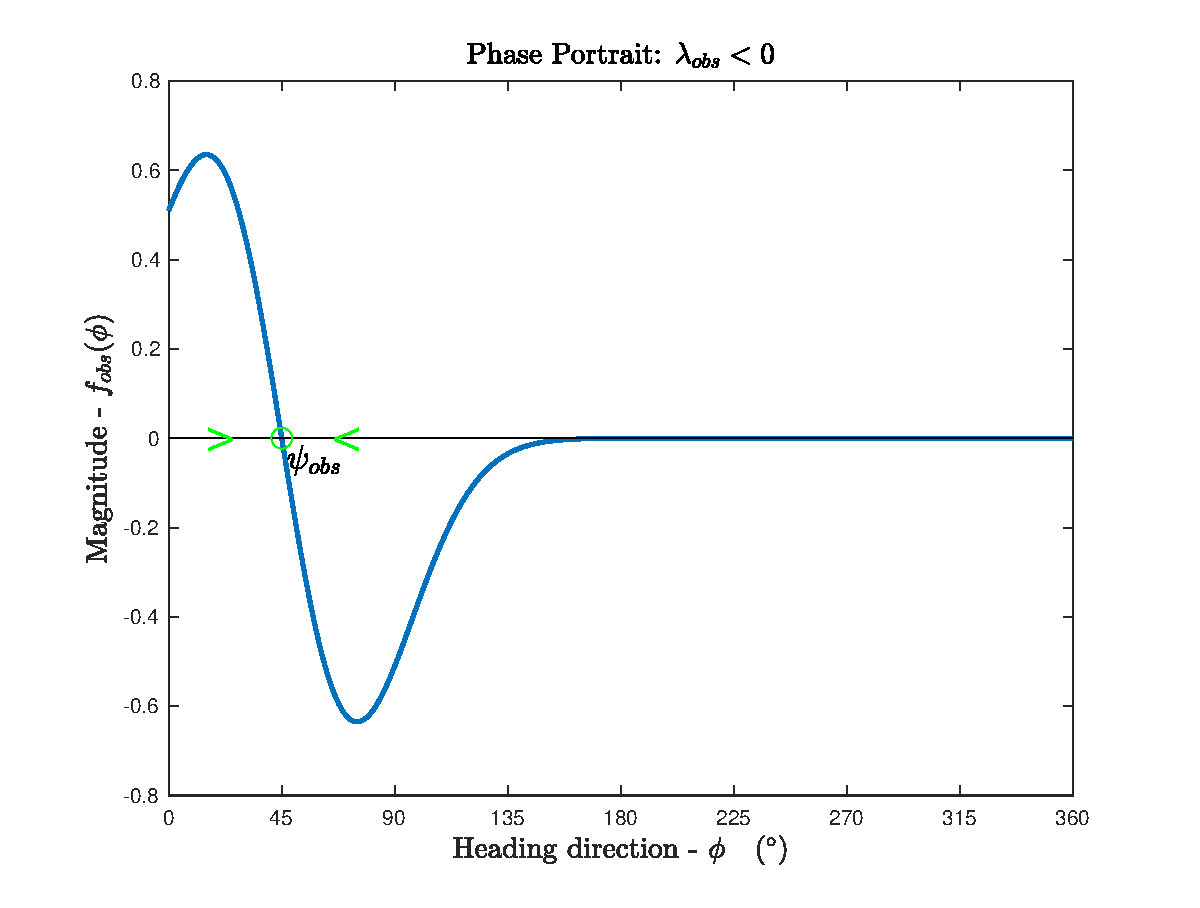
\includegraphics[width=1.0\textwidth]{./img/obs-phase-portrait-1.eps}
  \caption{$\lambda_{obs} < 0$: attractor}%
  \label{fig:obs-phase-port-1}
\end{subfigure}%
\begin{subfigure}{.5\textwidth}
  \centering
  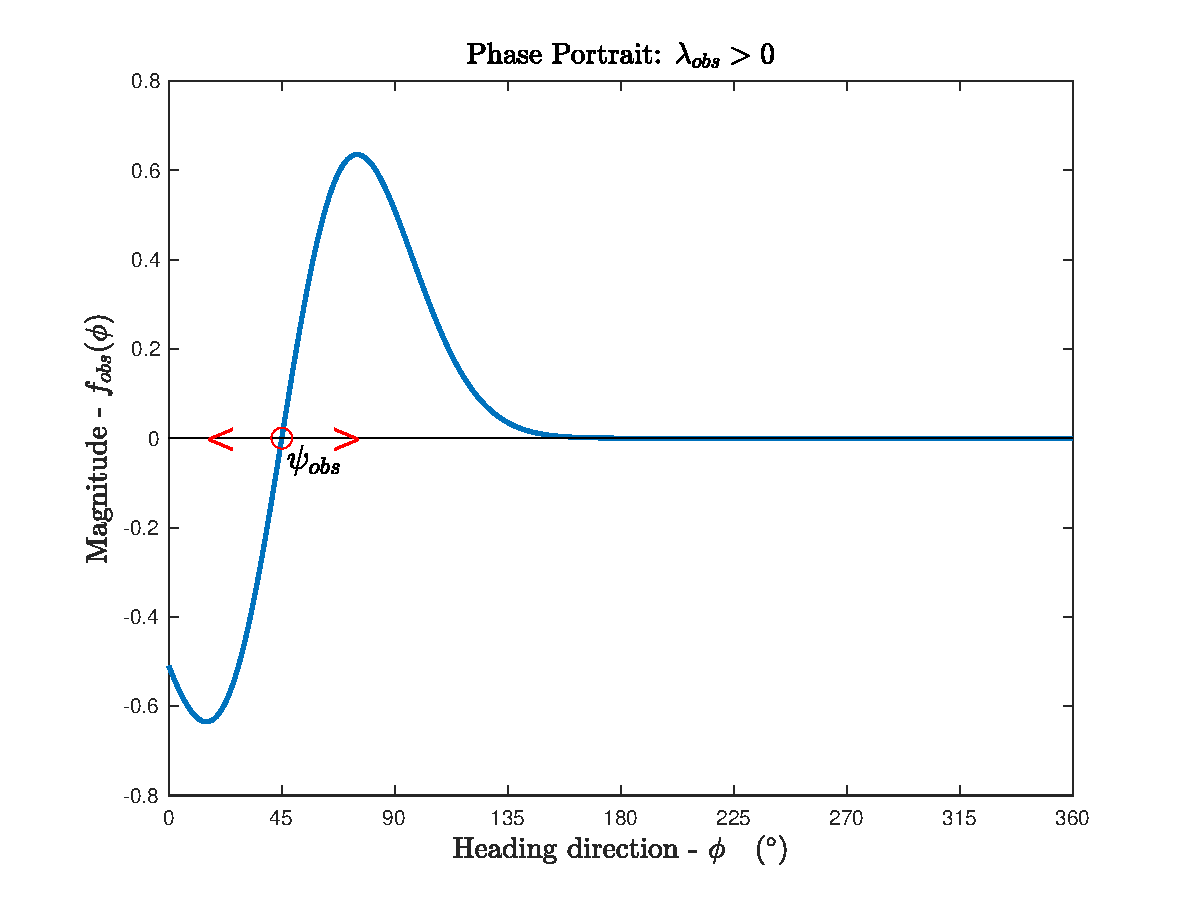
\includegraphics[width=1.0\textwidth]{./img/obs-phase-portrait-2.eps}
  \caption{$\lambda_{obs} > 0$: repeller}%
  \label{fig:obs-phase-port-2}
\end{subfigure}
\caption{Obstacle avoidance behavior: Phase portraits}%
\label{fig:obs-phase-portraits}
\end{figure}
%
\subsection{Bifurcation diagram}%
\label{sec:bifurcation-diagram-obs}
Fig.~\ref{fig:1-4-obs-bifurcation-diag} depicts the bifurcation diagram for the
target acquisition dynamic system, as a function of the parameter
$\lambda_{obs}$ $( \psi_{tar} \in [0, 2 \pi[ )$:
\begin{itemize}
\item $\lambda_{obs} < 0$: the fixed point $\phi^*$ is asymptotically stable.
\item $\lambda_{obs} > 0$: the fixed point $\phi^*$ is unstable.
\end{itemize}
%
$\lambda_{obs} = 0$ is a bifurcation point. This represents a transcritical bifurcation as there is an exchange in the
stability in the fixed point.
%
% Bifurcation diagram
\begin{figure}[!hbt]
\centering
    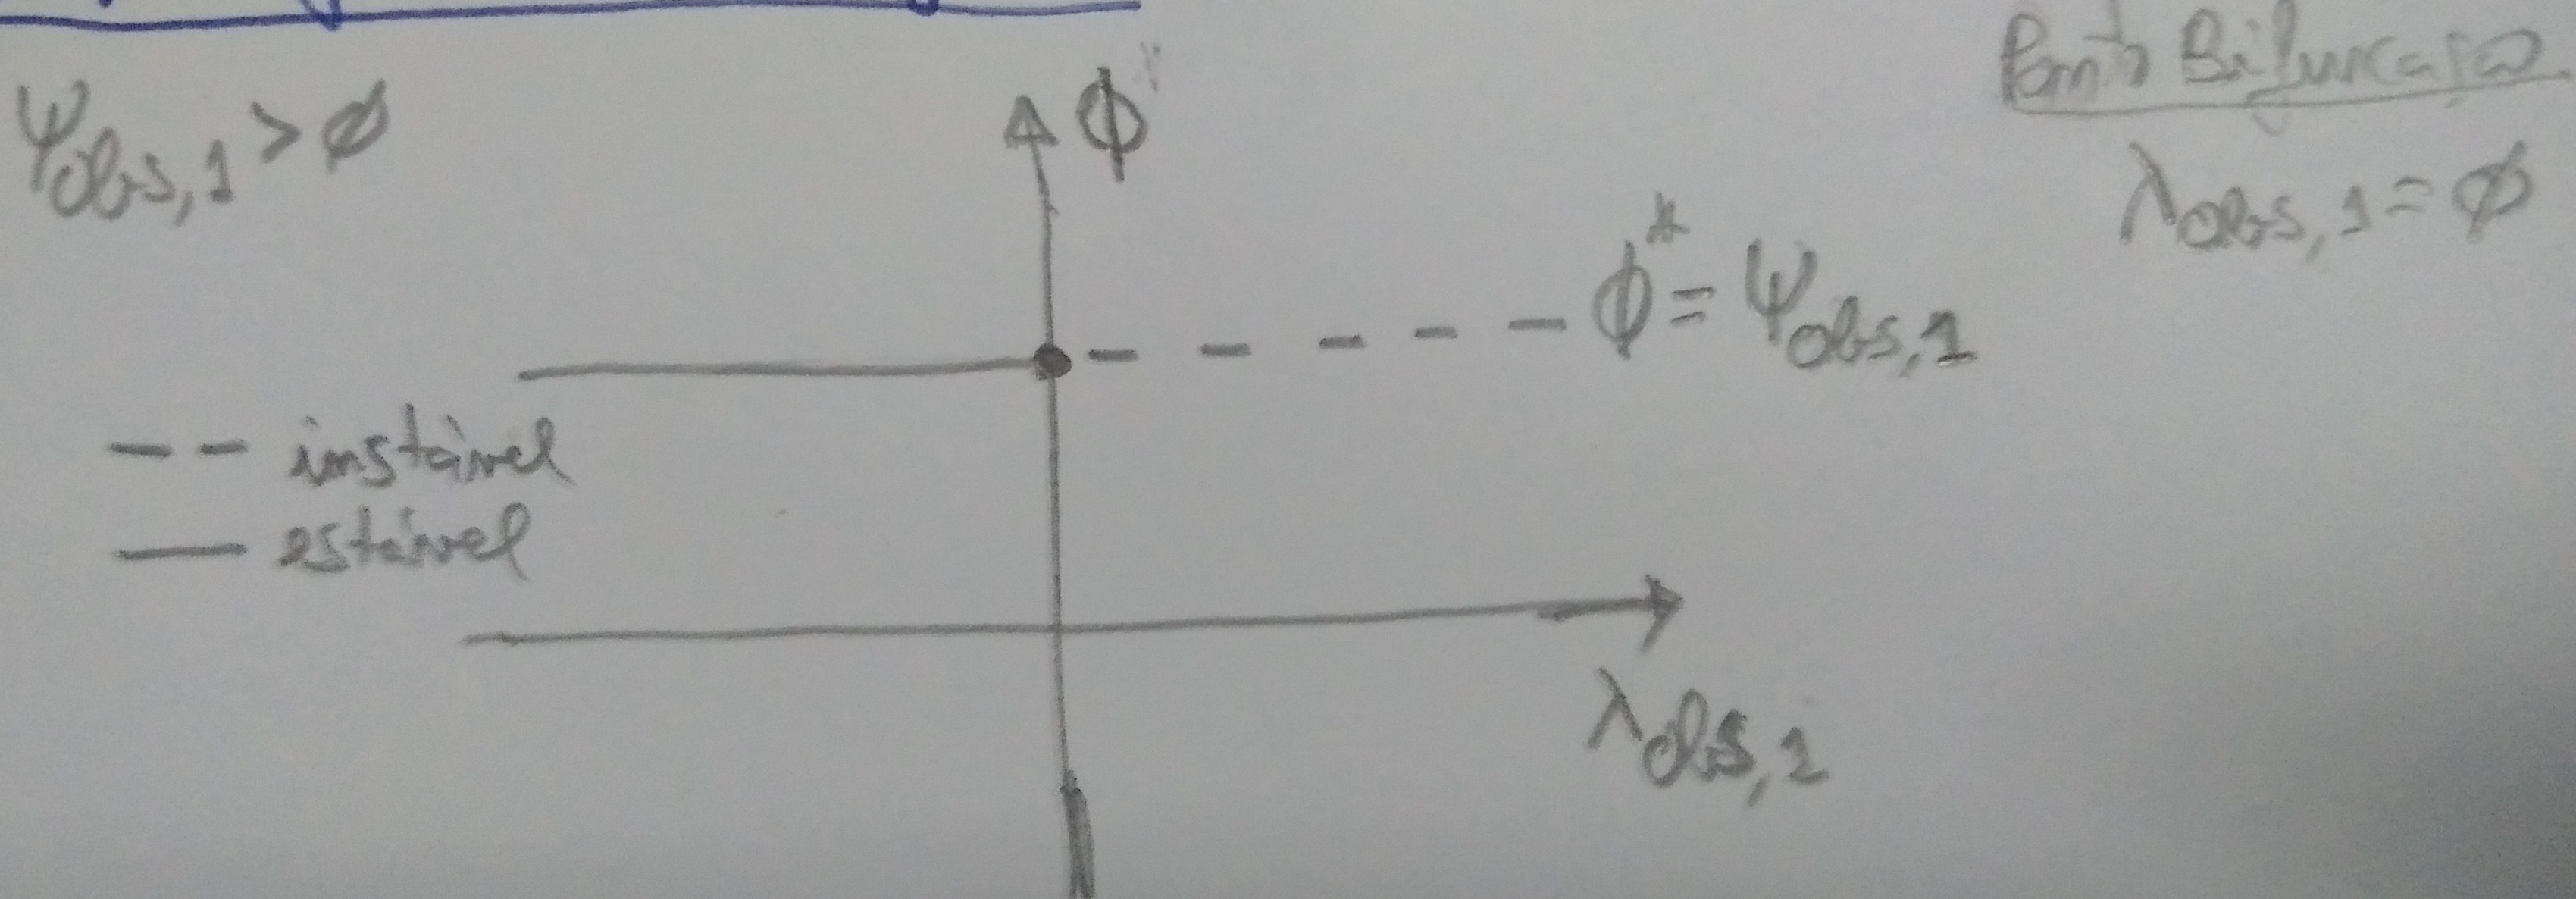
\includegraphics[width=0.6\textwidth]{./img/obs-bifurcation-diag.jpg}
  \caption{Obstacle behavior: Bifurcation diagram}%
\label{fig:1-4-obs-bifurcation-diag}
\end{figure}
%
%
\subsection{Range of values for $\beta_1$}%
\label{sec:range-values-beta1}
The parameter $\beta_1$ represents the maximum strength of the repulsive
forcelet, given by:
\begin{equation}
  \label{eq:32}
  \beta_1 = \max( \lambda_{obs,i} ) = \frac{1}{\min( \tau_{obs,i} )}
\end{equation}
i.e., is the inverse of the minimum time constant, $\gls{tau-obs-i}$, between all sensors.
The minimum time constant must be much greater than the Euler's step, $\Delta
t$, and considering reasonable boundaries, one has: 
\begin{equation}
  \label{eq:33}
 5 \Delta t < min(\tau_{obs}) <  10 \Delta t 
\quad \leftrightarrow \quad  
 \frac{1}{10  \Delta t} < \beta_1 <  \frac{1}{5 \Delta t}
\end{equation}
%
\subsection{Repulsion time constant}%
\label{sec:repuls-time-const}
This was previously calculated (see Section~\ref{sec:stability-obs}). 
%It should be noted, however, that for the overall obstacle avoidance dynamics,
%the repulsion time constant is calculated as the sumation of all time constants:
%\begin{equation}
%  \label{eq:33}
% m = \sum_{i = 1}^N {f'_{obs, i} (\phi_i^*)} = \sum_{i = 1}^N {\lambda_{obs, i}}= \lambda_{tot}
%\quad \leftrightarrow \quad
%\tau_{obs} = \frac{1}{\lambda_{tot}} = \frac{1}{\sum_{i=1}^N{\tau_{obs,i}}}
%\end{equation}
%
%
\section{Implementation}%
\label{sec:implementation-obs}
In this section, the implementation of the nonlinear dynamic system for obstacle
avoidance and simulation in CoppeliaSim using scenario
\texttt{MobileRobotDyn\_Tar\_Obs.ttt} is described for several different environment
scenarios. This aided the comprehension of the influence of several parameters
and enabled its successfull tuning, yielding the desired obstacle avoidance
behavior for the robot.

The first step of the implementation is to convert the first order differential
equation into an algebraic recursive equation by applying the forward Euler's
method in a discrete form:
\begin{equation}
  \label{eq:34}
  \phi(t + \Delta t) = \phi(t) + \Delta t F_{obs}(\phi), \qquad \phi(t_0) = \phi_0
\end{equation}
where $\Delta t$ is the Euler's step --- the incremental timestep applied to
the recursive equation and $F_{obs}(\phi)$ is given by Eq.~(\ref{eq:27}).
Simplying, both components of the dynamic system, $f_{obs}$ and $f_{stoch}$ can be
computed separately using Eqs.~(\ref{eq:35}) and~(\ref{eq:6}) and added,
yielding the complete dynamic system as given by Eq.~(\ref{eq:27}). Next, the
angular velocity of the vehicle can be determined, noting that $\omega _{robot}
= d \phi /dt$, i.e., equal to the complete vector field.

For smooth variation of the heading direction the
Euler's step must be significantly smaller than the minimum time constant (in
this case, the repulsion time), i.e., $\Delta t \ll \min(\tau _{obs})$, as
previously determined.

Next, for each sensor are computed the contribution to the repulsive force-let,
namely the direction the obstacle is seen, $\psi_{obs,i}$, magnitude of repulsion,
$\lambda_{obs,i}$, the range of repulsion, $\sigma_i$, and the effective
contribution to the repulsive forcelet, $f_{obs,i}$. The latter is accumulated,
yielding $f_{obs}$.

Finally, linear velocity is defined, and, if desired a stop criterion for the
distance to target. Then, the values of the angular and linear velocities of the
robot can be passed as setpoints to the low-level code responsible for
controlling these control variables.

Summarizing, the pseudocode for the obstacle avoidance behavior is as follows:
\begin{enumerate}
\item Initialize robot: retrieve simulation timestep and robot characteristics
\item Set initial values (linear and angular velocities) and set robot's initial
  pose ($x_{robot}, y_{robot}, \phi_{robot}$)
\item Define global parameter values: $N$, $\beta_2$, $Q$
\item Compute angular sector: $\Delta \theta = \theta_{obs,2} - \theta_{obs,1}$
\item Initialize target
\item While target <= targetNr
  \begin{enumerate}
  \item Exchange information with the simulator
  \item Get vehicle's pose, target position and simulation timestep
  \item Trigger a simulation step
  \item Processing step
    \begin{enumerate}
    \item Set parameters values: $\tau_{tar}, \lambda_{tar}, Q$
    \item For each sensor, compute the contribution of the repulsive forcelet
      \begin{enumerate}
      \item Compute $\psi_{obs,i}$, $\lambda_{obs,i}$, $\sigma_i$
      \item Compute $f_{obs,i}$
      \item Compute $f_{obs} = f_{obs} + f_{obs,i}$
      \end{enumerate}
    \item Compute $f_{obs}$ and $f_{stoch}$
    \item Compute resultant vector field $f_{total}$ and assign it to angular
      velocity
    \item Set linear velocity
    \item Define stop criterion for target distance (if desired)
    \end{enumerate}
  \item View dynamics: plot the obstacle avoidance dynamics
  \item Set robot's angular and linear velocities
  \end{enumerate}
\item Terminate simulation and cleanup
\end{enumerate}

As a result, the following generic Matlab code was implemented (Listing~\ref{lst:program-dyn-obs}):
% program_dyn_tar.m (generic)
\lstinputlisting[language=matlab, caption={Generic implementation of obstacle
  avoidance behavior (not tuned)},label=lst:program-dyn-obs,
style=custom-matlab]{./listing/program_dyn_obs.m}%

\subsection{Scenario 1}%
\label{sec:scenario-1-obs}
The obstacles were placed at a distance of 0 cm between each other to form a
wall (no gap). The robot was
placed in the middle of the arena and facing the wall at a distance of 100 cm. The stochastic force was
reset (null variance --- $Q = 0$). The robot moves at a constant linear velocity
of 20 cm/s, which is a reasoable value. The  parameter $\beta_2 = 20$ was fixed
and $\beta_1$ was increased until the robot avoids collision with the wall.
Then, for each value of $\beta_1$, the contribution of each sensor and the
resultant obstacle avoidance dynamics were observed.

$\beta_1$ is related to $\min(\tau_{obs,i})$ (Eq.~(\ref{eq:32})), thus,
\texttt{tau\_obs\_min} was set, starting from $10 \Delta t$ and
decremented at unit steps. Fig.~\ref{fig:obs-2-1-arena-fail} illustrates the
simulation for \texttt{tau\_obs\_min} = $5 \Delta t$, where a collision occurs
with a wall (robot becomes red). 
%
\begin{figure}[!hbt]
\centering
    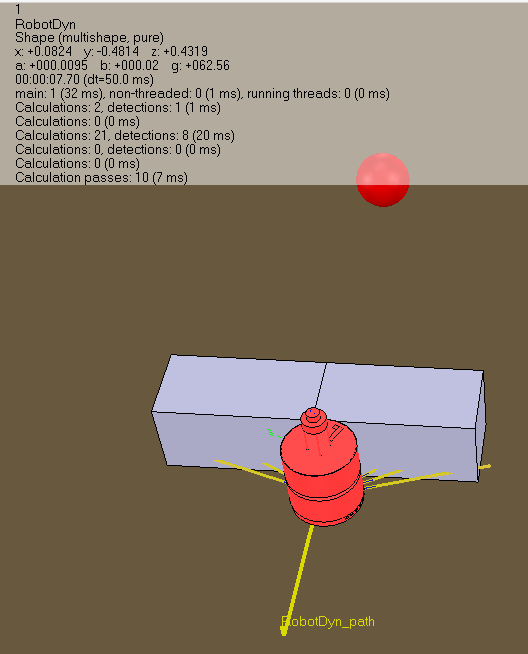
\includegraphics[width=0.55\textwidth]{./img/obs-2-1-arena-fail.png}
  \caption{Obstacle avoidance behavior: \texttt{tau\_obs\_min} = $5 \Delta t$}%
\label{fig:obs-2-1-arena-fail}
\end{figure}

Conversely, in
Fig.~\ref{fig:obs-2-1-arena-success} is illustrated the final state of the first
compliable value of $beta_1$ for collision-free path (\texttt{tau\_obs\_min} =
$4 \Delta t$), as indicated by the auxiliary text 
(see also Video \href{run:./videos/obs-2-1.mp4}{./videos/obs-2-1.mp4}). 
In the obstacle avoidance
dynamics plot it can be observed that, in the final state depicted, the heading
direction is very far appart from the repeller, as expected. 
%
\begin{figure}[!hbt]
\centering
    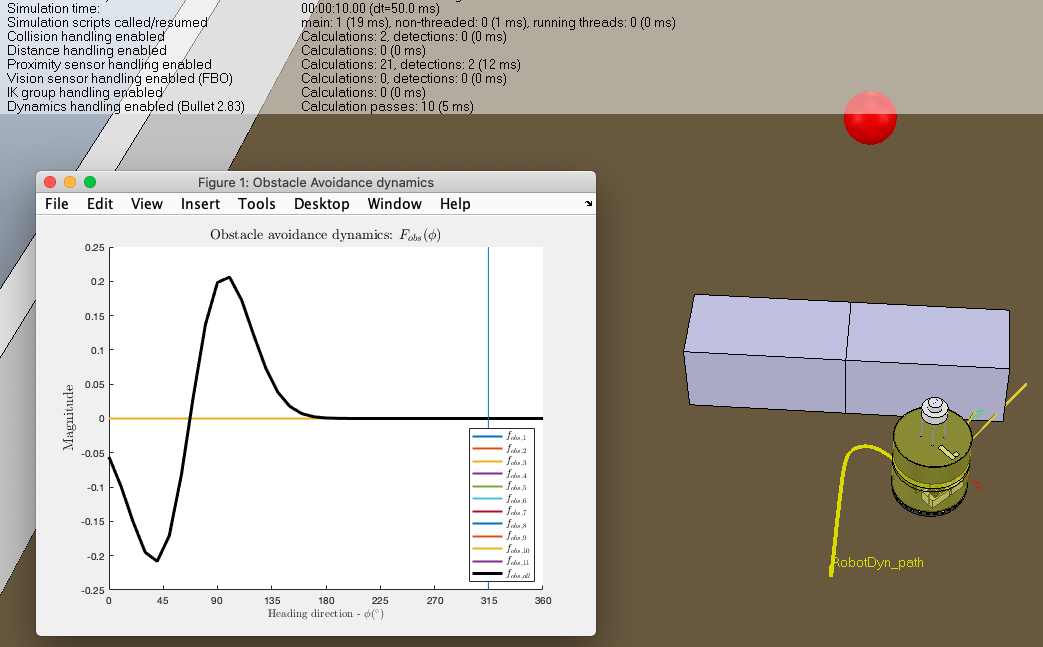
\includegraphics[width=0.9\textwidth]{./img/obs-2-1-arena-success.png}
  \caption{Obstacle avoidance behavior: \texttt{tau\_obs\_min} = $4 \Delta t$ (final state)}%
\label{fig:obs-2-1-arena-success}
\end{figure}

The deviation from
the obstacles only happened when the strenght of the repeller was
sufficiently high to induce significant angular velocities, which for this case,
started at $\omega = d\phi/dt = -0.5$ rad/s and hit its maximum at approximately
$\omega = -3$ rad/s, representing an counterclockwise turn. It is important to note, however, that this calibration for
collision-free path of the parameter $\beta_1$ is dependent on the value of the
linear velocity, as the system may not have time to react to it --- the higher
the value of the linear velocity (constant), the lower the value of
\texttt{tau\_obs\_min} needs to be. On the other hand, the linear velocity
should decrease with the distance to the obstacles, which could be modelled as a
dynamic system, e.g., the one in Eq.~(\ref{eq:12}).

Fig.~\ref{fig:obs-scenario1-facing-front} shows in more detail the obstacle
avoidance dynamics plot, used as an aiding tool, with the robot direction
direction still facing the wall, i.e., $\phi = \psi_{obs}$. It can be seen that
5 sensors are detecting the obstacles, yielding a stronger reppeller in that
direction, but still insufficient for significant direction change.
%
\begin{figure}[!hbt]
\centering
    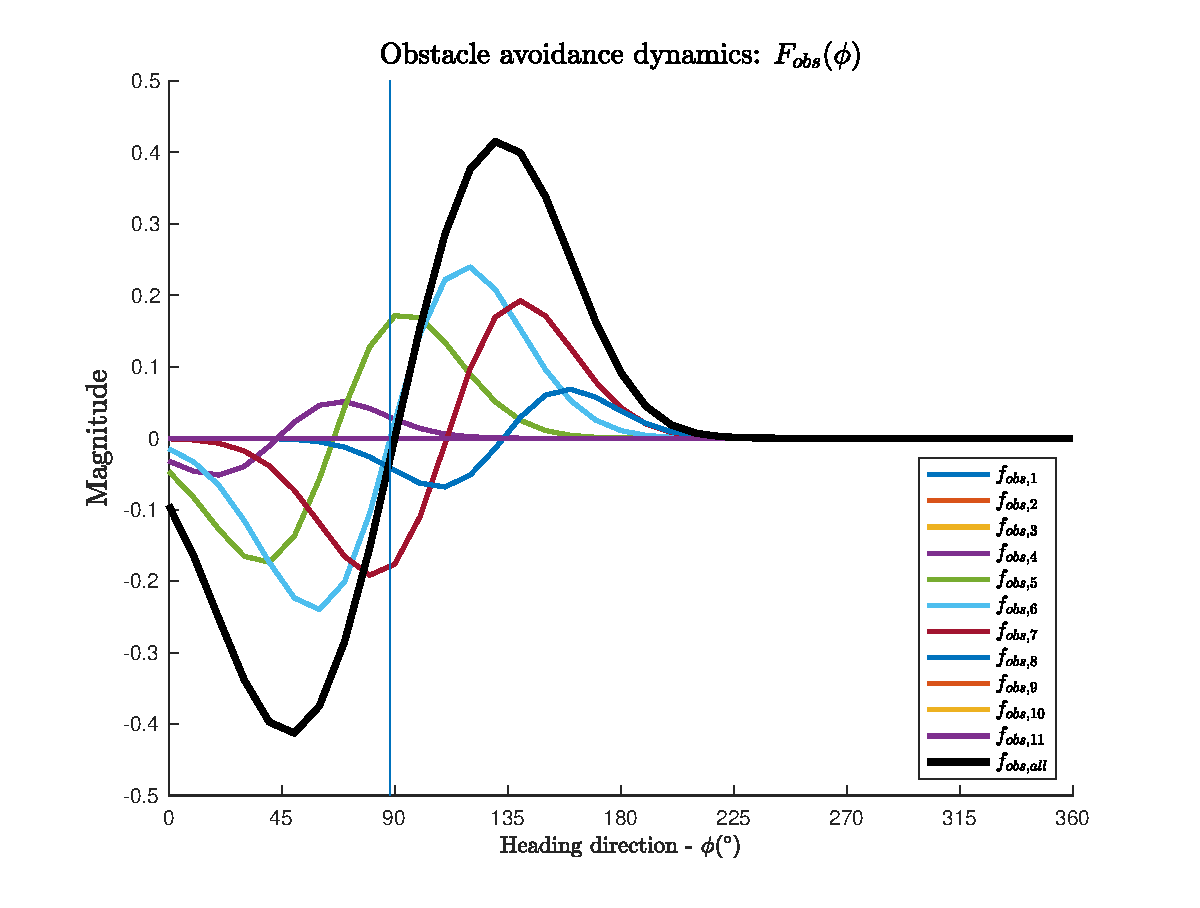
\includegraphics[width=0.7\textwidth]{./img/obs-scenario1-facing-front.eps}
  \caption{Obstacle avoidance behavior: dynamics --- \texttt{tau\_obs\_min} = $4 \Delta t$}%
\label{fig:obs-scenario1-facing-front}
\end{figure}

The addition of noise to the dynamic system was unnecessary, as there is a
slight bias from sensors readings, due to uneven obstacle detection by all
sensors --- the leftmost sensors did not detect the obstacles initially, whereas
the rightmost did. This slight bias for obstacles detection is responsible for
the counterclockwise turn, rendering it unnecessary to incorporate noise for the
robot to deviate from the obstacles, albeit the heading direction initially sits in a repeller.
%
%
\subsection{Scenario 2}%
\label{sec:scenario-2-obs}
The obstacles were now placed at a 10 cm gap between each other, 
and the robot was
placed in the middle of the arena facing the gap at a distance of 100 cm. 
The remaining conditions from scenario 1 remained unchanged.

First, the system was simulated with the previous value of $\beta_1$ to assess
the system's behavior (Fig.~\ref{fig:obs-2-2-1}). It can be seen that the robot
collides with an obstacle in the attempt to deviate from it, as the heading
direction still remains inside the influence of repellers. 
%
\begin{figure}[!hbt]
\centering
    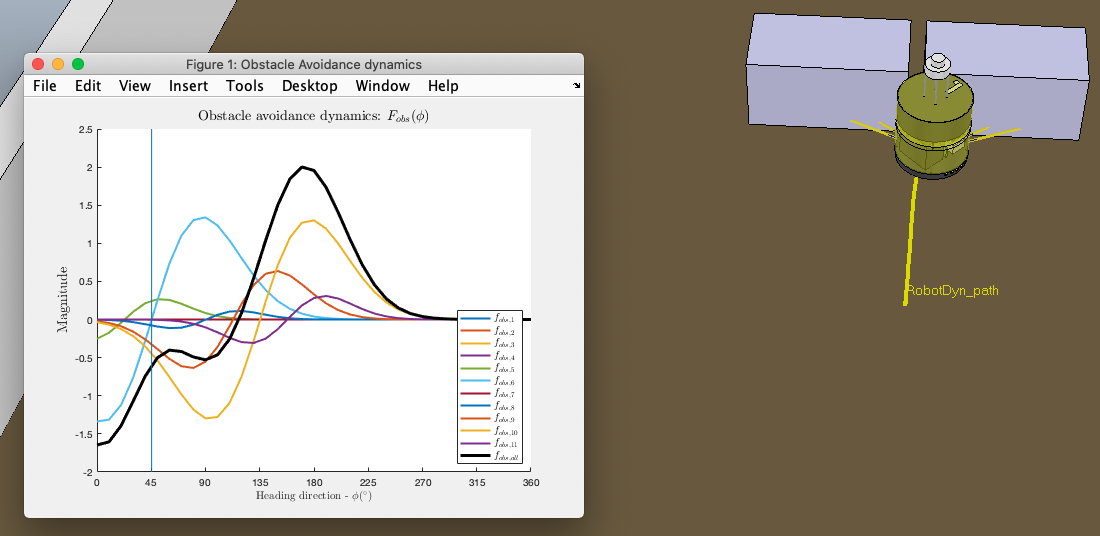
\includegraphics[width=0.7\textwidth]{./img/obs-2-2-1.png}
  \caption{Obstacle avoidance behavior: dynamics --- \texttt{tau\_obs\_min} = $4
    \Delta t$, gap = 10 cm}%
\label{fig:obs-2-2-1}
\end{figure}

It does not detect obstacles in most of the path in the most central sensor, as it moves forward, due to the gap, which was
the most strong contribution. When the contributions of the other sensors are
high enough to trigger robot's rotation, the robot starts to rotate
(counterclockwise, in this case), but the dynamics is not fast or strong enough
to avoid the obstacle.

The value of parameter $\beta_1$ was then retuned to avoid collisions with the
obstacles, following the same procedure, i.e., decrementing
\texttt{tau\_obs\_min}. Fig.~\ref{fig:obs-2-2-2} illustrates the first
collision-free path of the robot with the new environment conditions, occurring
at \texttt{tau\_obs\_min} = $3.5 \Delta t$ (see also Video
\href{run:./videos/obs-2-2.mp4}{./videos/obs-2-2.mp4}).
%
\begin{figure}[!hbt]
\centering
    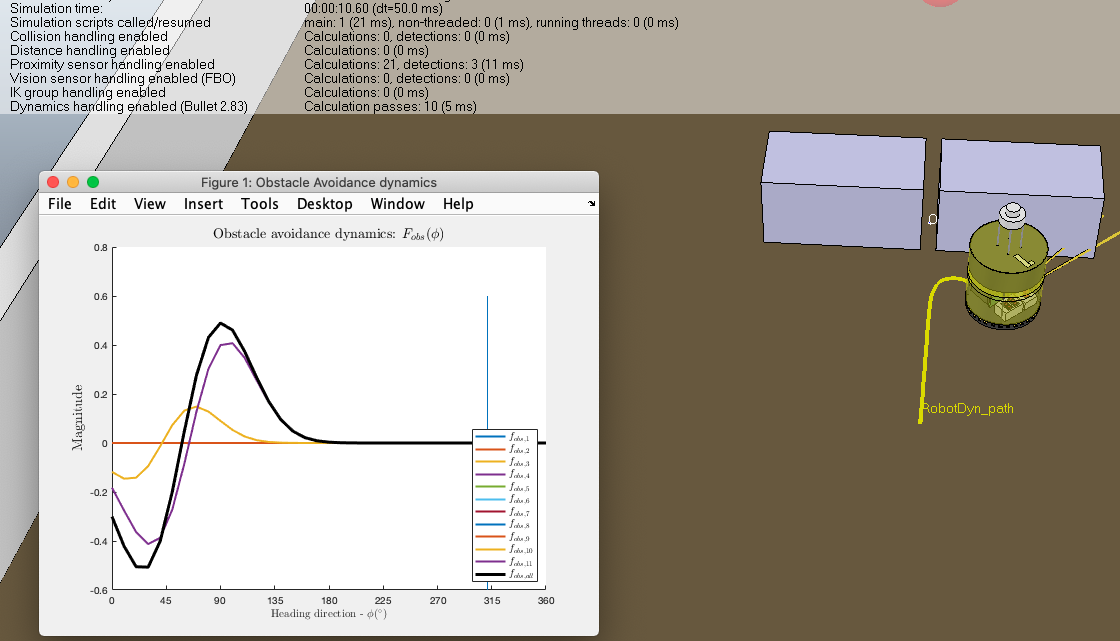
\includegraphics[width=0.7\textwidth]{./img/obs-2-2-2.png}
  \caption{Obstacle avoidance behavior: dynamics --- \texttt{tau\_obs\_min} =
    $3.5 \Delta t$, gap = 10 cm}%
\label{fig:obs-2-2-2}
\end{figure}
%
\subsection{Scenario 3}%
\label{sec:scenario-3-obs}
In this scenario several simulations are performed for different gaps between
obstacles, namely 20--80 cm, with a 10 cm span. Fig.~\ref{fig:obs-2-3-50cm}
illustrates the first case where the robot can move between the obstacles, which
occurs for a distance gap of 50 cm between them.
(see also Video
\href{run:./videos/obs-2-3-50cm.mp4}{./videos/obs-2-3-50cm.mp4}). Fig.~\ref{fig:obs-2-3-50cm-2}
shows that for a 50 cm gap, in the situation depicted in Fig.~\ref{fig:obs-2-3-50cm-1}, the heading direction has an attractor, instead of a
repeller (0--40 cm), and two repellers at approximately 60$^{\circ}$ and 120$^{\circ}$.
%
\begin{figure}[!hbt]
\centering
\begin{subfigure}{.5\textwidth}
  \centering
  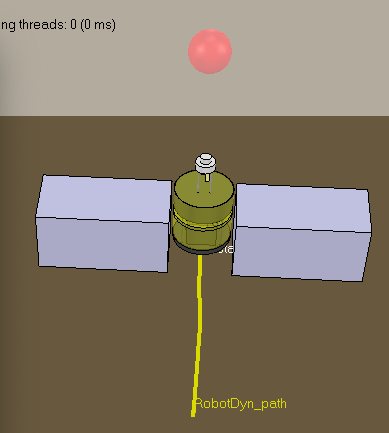
\includegraphics[width=0.7\textwidth]{./img/obs-2-3-50cm-1.png}%
  \caption{Simulation}%
\label{fig:obs-2-3-50cm-1}
\end{subfigure}%
\begin{subfigure}{.5\textwidth}
  \centering
  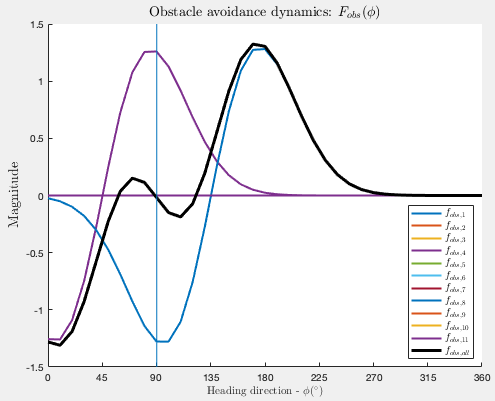
\includegraphics[width=1.0\textwidth]{./img/obs-2-3-50cm-2.png}%
  \caption{Dynamics}%
\label{fig:obs-2-3-50cm-2}
\end{subfigure}
  \caption{Obstacle avoidance behavior: dynamics --- \texttt{tau\_obs\_min} =
    $3.5 \Delta t$, gap = 50 cm}%
\label{fig:obs-2-3-50cm}
\end{figure}
%
\subsection{Bifurcation analysis}%
\label{sec:bifurcation-analysis-obs}
As indicated in Section~\ref{sec:scenario-3-obs}, the heading direction dynamics
exhibits different qualitative behavior --- the stability of the fixed
points varies --- starting from gap = 50 cm. This corresponds to a bifurcation
point, representing the distance below which the robot
(with diameter 45 cm) cannot pass between the two obstacles. For gap < 50 cm, the planning dynamics has an reppeller
at the heading direction $\phi = \pi/2$, and for gap > 50 this reppeller becomes
asymptotically stable (i.e., an attractor).

\subsection{Influence of parameter $\beta_2$}%
\label{sec:infl-param-beta2}
The parameter $\beta_2$ is the decay rate of the repulsion force with the
distance increase. Thus, to test this, $\beta_2$ was varied and simulated in the
conditions of scenario 1, and the resulting repulsion magnitude
$\lambda_{obs,i}$ computed (see Fig.~\ref{fig:obs-2-5}). 
%
\begin{figure}[!hbt]
\centering
\begin{subfigure}{.5\textwidth}
  \centering
  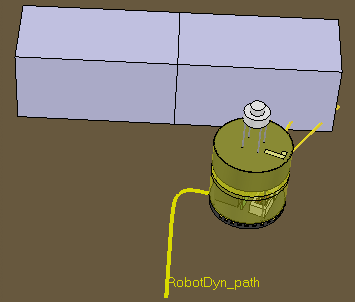
\includegraphics[width=0.7\textwidth]{./img/obs-2-5-beta2-50.png}%
  \caption{$\beta_2 = 50$}%
\label{fig:obs-2-5-beta-2-50}
\end{subfigure}%
\begin{subfigure}{.5\textwidth}
  \centering
  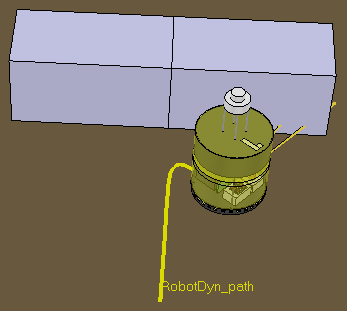
\includegraphics[width=0.7\textwidth]{./img/obs-2-5-beta2-15.png}%
  \caption{$\beta_2 = 15$}%
\label{fig:obs-2-5-beta2-15}
\end{subfigure}
  \caption{Obstacle avoidance behavior: influence of parameter $\beta_2$}%
\label{fig:obs-2-5}
\end{figure}

For increasing values of $\beta_2$ (Fig.~\ref{fig:obs-2-5-beta-2-50}), the decay rate
diminishes, maintaining the repulsive effect significantly for
a wider distance range --- the robot starts to rotate farther away from the obstacles.
Conversely, for decreasing values of $\beta_2$ (Fig.~\ref{fig:obs-2-5-beta2-15}), the decay rate
increases, maintaining the repulsive effect significantly for
a narrow distance range --- the robot starts to rotate closer to the obstacles.

\subsection{Influence of noise}%
\label{sec:influence-noise-obs}
The influence of noise was tested, varying the value of the magnitude of
gaussian white noise, $Q$ (see Fig.~\ref{fig:obs-2-6}).
%
\begin{figure}[!hbt]
\centering
\begin{subfigure}{.5\textwidth}
  \centering
  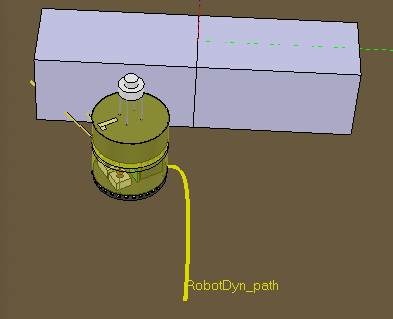
\includegraphics[width=0.76\textwidth]{./img/obs-2-6-Q-005.png}%
  \caption{$\beta_2 = 15, Q = 0.05$}%
\label{fig:obs-2-6-Q-005}
\end{subfigure}%
\begin{subfigure}{.5\textwidth}
  \centering
  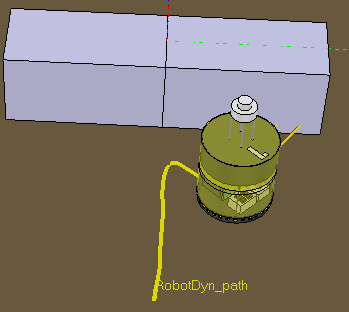
\includegraphics[width=0.7\textwidth]{./img/obs-2-6-Q-05.png}%
  \caption{$\beta_2 = 15, Q = 0.5$}%
\label{fig:obs-2-6-Q-05}
\end{subfigure}
  \caption{Obstacle avoidance behavior: influence of noise}%
\label{fig:obs-2-6}
\end{figure}

Comparing Fig.~\ref{fig:obs-2-6-Q-005} with Fig.~\ref{fig:obs-2-5-beta2-15}, it
can be seen that the mere introduction of noise induced a different qualitative
behavior with the decision of turning left instead of right,
respectively. Additionally, in Fig.~\ref{fig:obs-2-6-Q-05}, it can be seen the
magnitude of noise should be maintained fairly low, as it may introduce jitter
into the system, depicted by the less `clean' path. Thus, the noise should be
sufficient to enough to guarantee the escape from the repellers within a time
limit, in case the system is initially placed there.

\subsection{Scenario 4}%
\label{sec:scenario-4-obs}
Fig.~\ref{fig:obs-2-7} illustrates scenario 4, composed of several obstacles
that the robot must avoid. It can be observed that the robot is able to avoid
all obstacles, as expected.

\begin{figure}[!hbt]
\centering
    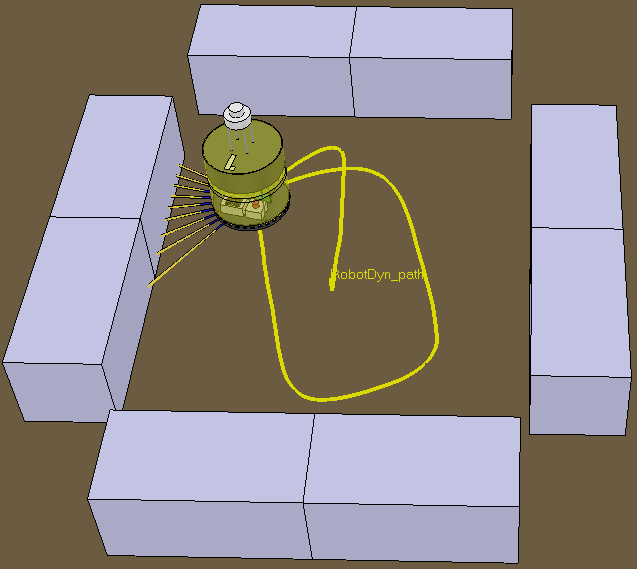
\includegraphics[width=0.6\textwidth]{./img/obs-2-7.png}
  \caption[Obstacle avoidance behavior: Simulation with several obstacles]{Obstacle avoidance behavior: Simulation with several obstacles --- \texttt{tau\_obs\_min} =
    $3.5 \Delta t$, Q = 0.05, $\beta_2 = 20$}%
\label{fig:obs-2-7}
\end{figure}
%%% Local Variables:
%%% mode: latex
%%% TeX-master: "../../dissertation"
%%% End:

  \setcounter{table}{0}
  \setcounter{figure}{0}
%  
  \renewcommand{\baselinestretch}{1.0}
\chapter{Integration of behaviors: Obstacle Avoidance and Target Acquisition (nonlinear)}%
\label{ch:obstacle-target-nonlinear}
\renewcommand{\baselinestretch}{1.5}
In this chapter the obstacle avoidance and target acquisition behaviors are
integrated, but for the latter is considered a nonlinear dynamic system. A
detailed analysis is then performed over: obstacle avoidance and target
acqusition time constant precedence and tuning; distance between obstacles and
respective bifurcation analysis; the influence of noise (stochastic force). 
Finally, more demanding scenarios are simulated, respectively in \emph{S} or
\emph{U} shape, and the robot's behavior is analyzed.

\section{Implementation}
The nonlinear dynamic system that controls the movement of the robot for target
acquisition in a collision-free path is obtained
through the sum of the obstacles and target dynamic systems contribuitions and
also a stochastic component for escaping repellers in a finite time, as given by Eq.~(\ref{eq:36}):
%
\begin{equation}
\label{eq:36}
 \frac{d \phi}{dt} = \sum_{i = 1}^N{f_{obs,i}(\phi)} + f_{tar}(\phi) + f_{stoch}
\end{equation}

Thus, the implementation is simply the sum of these components (see Listing~\ref{lst:program-dyn-obs-tar-nonlinear}).
% program_dyn_tar.m (generic)
\lstinputlisting[language=matlab, caption={Implementation of obstacle
  avoidance behavior and target acquisiton},label=lst:program-dyn-obs-tar-nonlinear,
style=custom-matlab]{./listing/program_dyn_obs_tar_nonlinear.m}%

However, as it will be discussed further ahead, the tuning of the overall system
parameters is critical for adequate collision-free navigation to the target. By
design, the obstacle avoidance behavior takes precedence over target
acquisition, as obviously, in a limit case --- e.g., where the target is behind an
obstacle --- the robot must circumvent the obstacle, instead of hitting it. This
is guaranteed by imposing higher magnitude for repulsive component than for
attractive one, i.e. $\lambda_{obs} \gg \lambda_{tar}$, and consequently,
$\tau_{obs} \ll \tau_{tar}$.

\section{Scenario 1}%
\label{obst-tar-nonlinear-scenario1}
In this section are analyzed the influences of varying the magnitude of
attraction to target, $\lambda_{tar}$, the distance between obstacles, and the noise
(stochastic force) in the robot's navigation behavior.

\subsection{Magnitude of attraction to target: $\lambda_{tar}$}%
\label{obst-tar-nonlinear-lambda-tar}
If the magnitude of the target is greater than the obstacles, the
issue that occurs is that it is only when the robot is a very short distance
from the obstacle that the repeller is established. When the robot is close to
the obstacle this one is detected in several directions and the sum of these
repulsive forces exceeds the force of attraction, changing the stability of the
fixed point of that navigation direction (Fig~\ref{fig:obs-tar-nonlinear-different-lambda}).
%
\begin{figure}[htb!]
  \centering
  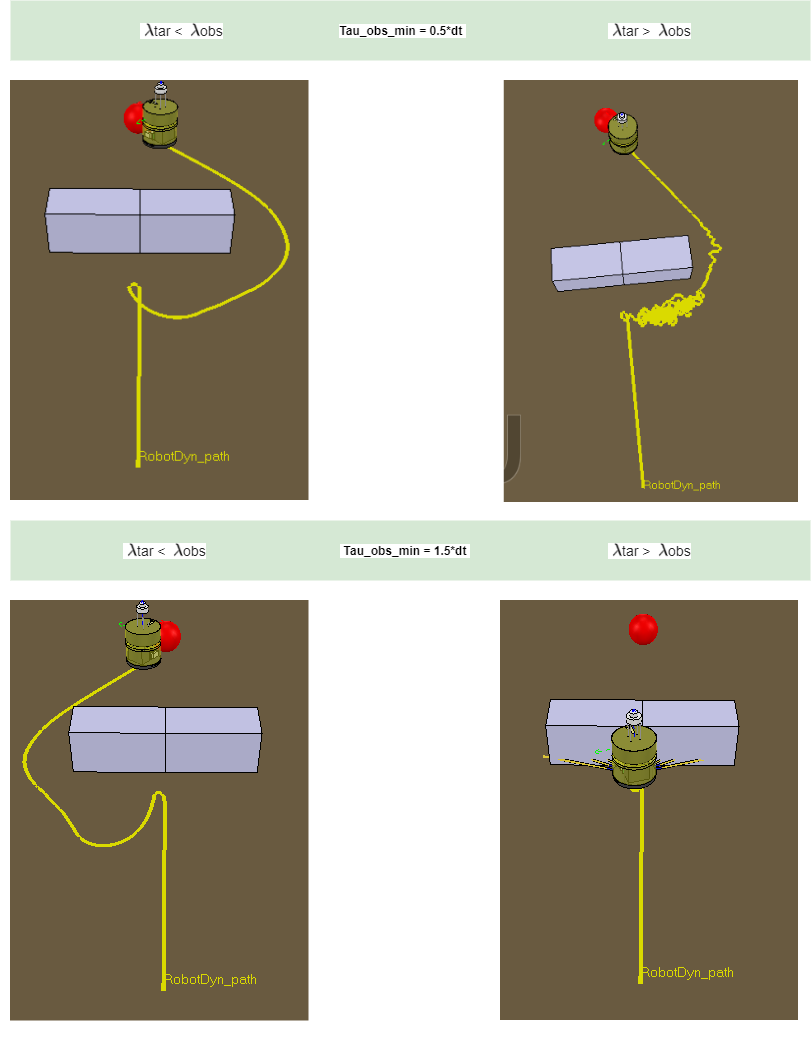
\includegraphics[width=0.6\textwidth]{img/ytar.png}
  \caption{Different $\lambda_{tar}$ values simulations results.}%
  \label{fig:obs-tar-nonlinear-different-lambda}
\end{figure}

Consequently, as shown in Fig.~\ref{fig:obs-tar-nonlinear-different-lambda}, or the robot collides with the obstacle or has a very irregular route, depending on the time constant. Having enough time to escape the repeller, the robot has a zigzag route, because it approaches the obstacle and moves away successively since it is only close to this that it realizes that there is an obstacle. If there is not enough time to change the heading direction, the robot collides.
Therefore, the magnitude of the repulsing from the obstacle must always be
greater than that of the attraction to
the target, i.e., 
$\lambda_{obs} \gg \lambda_{tar}$, and consequently, $\tau_{obs} \ll \tau_{tar}$.
%
\subsection{Different gaps between obstacles}
In this scenario, \texttt{MobileRobotDyn\_Tar\_Obs.ttt},
several simulations are performed for different gaps between obstacles, namely 0
cm, 10 cm and 50 cm span.

\subsubsection{No gap (0 cm)}%
\label{sec:Different-gaps-0cm}
Fig.~\ref{fig:obs-tar-nonlinear-behavioral} illustrates the simulations
performed for obstacles forming a wall without gap (0 cm).
%
\begin{figure}[htb!]
  \centering
  \begin{subfigure}{.45\textwidth}
  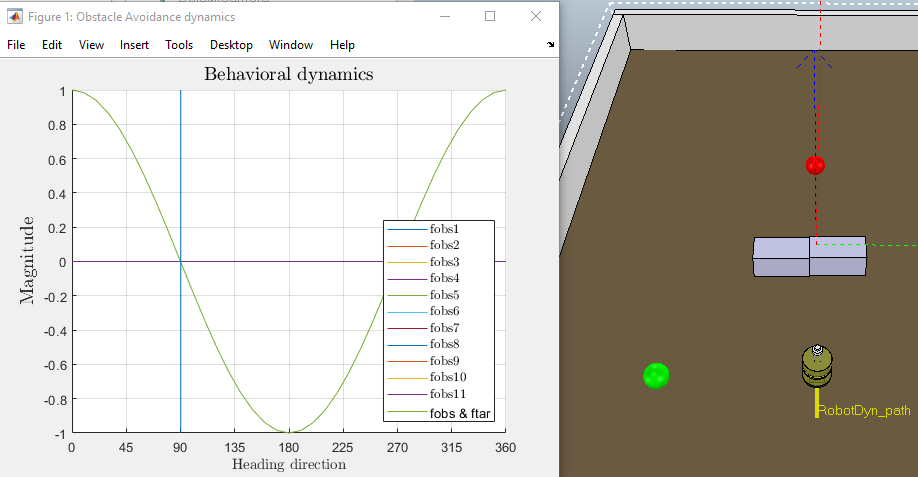
\includegraphics[width=\textwidth]{img/3-2-1.PNG}%
  \caption{}%
  \label{fig:obs-tar-nonlinear-behavioral-1}
  \end{subfigure}
  \begin{subfigure}{.45\textwidth}
    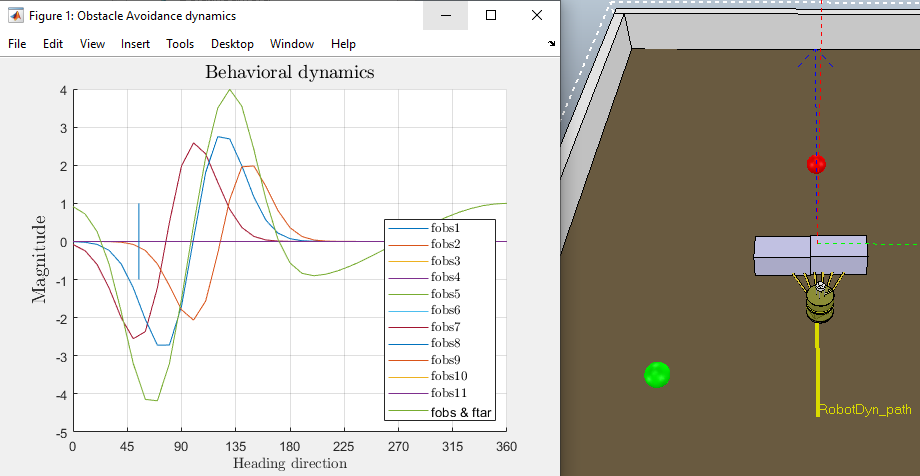
\includegraphics[width=\textwidth]{img/3-2-2.PNG}%
  \caption{}%
  \label{fig:obs-tar-nonlinear-behavioral-2}
  \end{subfigure}
  % 
  \begin{subfigure}{.45\textwidth}
    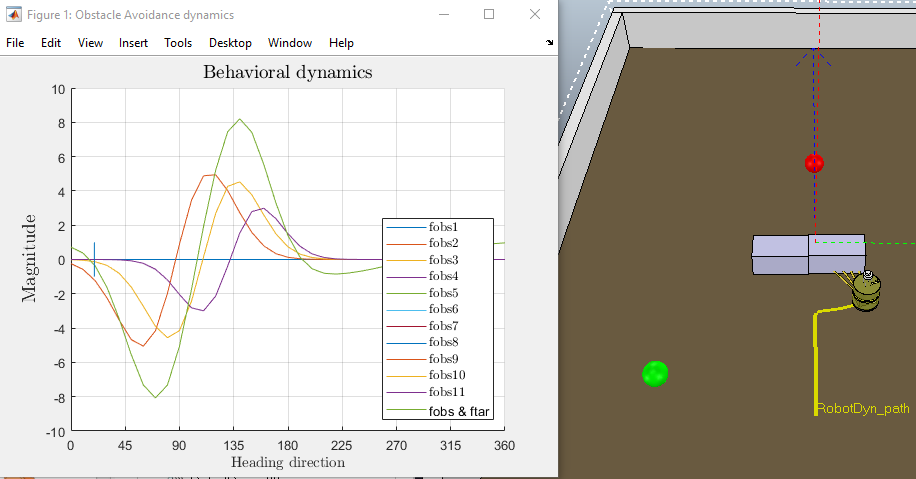
\includegraphics[width=\textwidth]{img/3-2-3.PNG}%
  \caption{}%
  \label{fig:obs-tar-nonlinear-behavioral-3}
  \end{subfigure}
  % 
  \begin{subfigure}{.45\textwidth}
    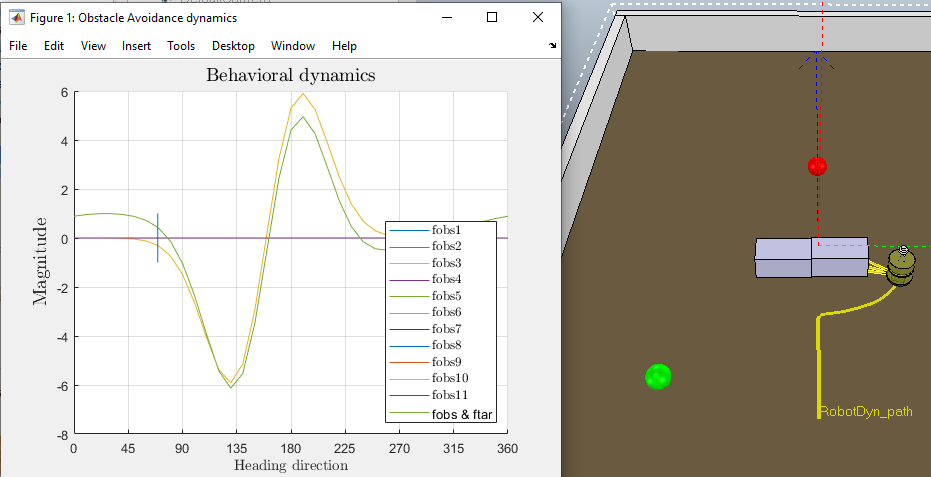
\includegraphics[width=\textwidth]{img/3-2-4.PNG}%
  \caption{}%
  \label{fig:obs-tar-nonlinear-behavioral-4}
  \end{subfigure}
  \begin{subfigure}{.45\textwidth}
    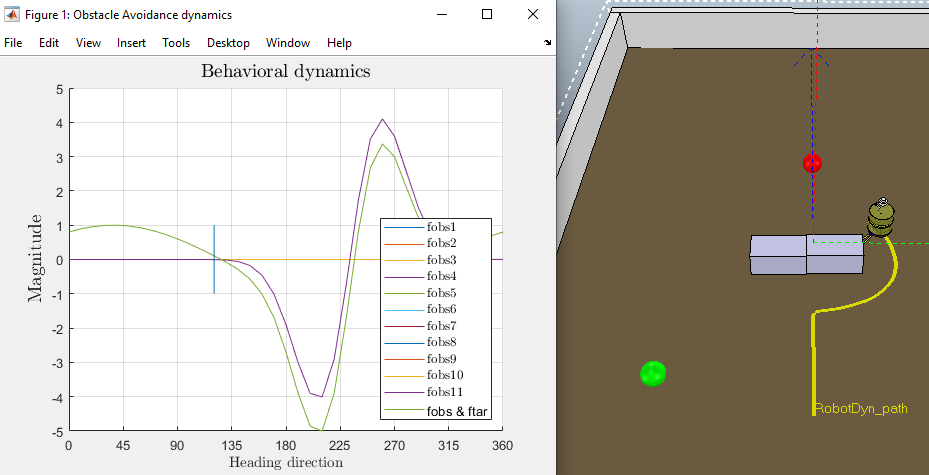
\includegraphics[width=\textwidth]{img/3-2-5.PNG}%
  \caption{}%
  \label{fig:obs-tar-nonlinear-behavioral-5}
  \end{subfigure}
  % 
  \begin{subfigure}{.45\textwidth}
    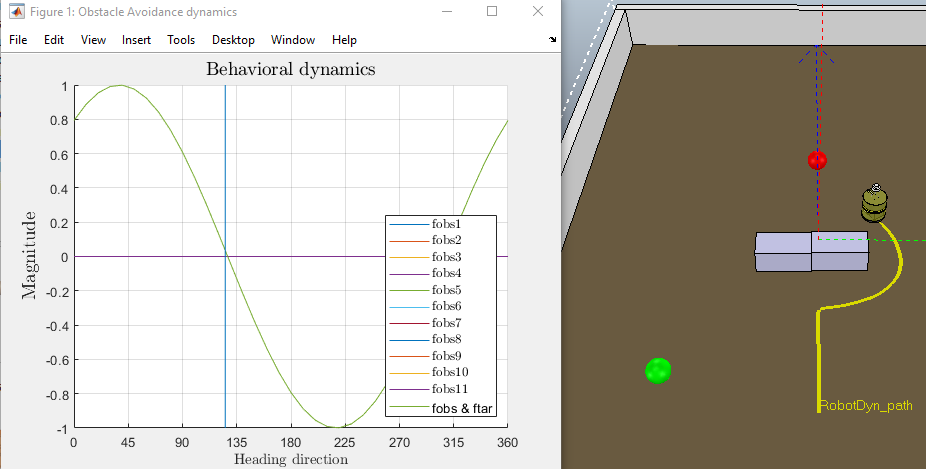
\includegraphics[width=\textwidth]{img/3-2-6.PNG}%
  \caption{}%
  \label{fig:obs-tar-nonlinear-behavioral-6}
  \end{subfigure}
  \caption{Behavioral Dynamics depending on the robot's position in the world}%
  \label{fig:obs-tar-nonlinear-behavioral}
\end{figure}

In the first simulation, the obstacles form a wall and the robot is
positioned in front of the obstacles but without the sensors detecting it. (Fig.~\ref{fig:obs-tar-nonlinear-behavioral-1}). 
The stochastic force is not considered and the parameter $\beta _{2}$ is 50.
In the initial moments, obstacles are not detected by the sensors, so they do
not contribute to the dynamics vector field in the navigation direction 
positioned in front of the obstacles but without the sensors detected.

As the robot approaches the wall, the sensors begin to detect obstacles, in the
first moments, due to the considerable distance to the obstacle, the repeller is
of low magnitude so it does not prevail, therefore an attractor is formed in the
direction of navigation, with a lower intensity of attraction than
before. However, as the distance to the obstacles decreases, it is visible that
the intensity of the repeller increases and dominates, an instability occurs,
the vector field of the dynamics of the navigation direction starts to have a
repeller in that direction. When the stability of the fixed points changes, it
because the bifurcation point has been exceeded, and the robot will present a
different behaviour than previous.

So such behavior is in line with expectations since with the proximity to an
obstacle the forces of repulsion
appear and prevail over attraction forces. Because of that the robot can escape from the obstacle to the right or
left, because there are two attractors in these directions, attending at the
Figs.~\ref{fig:obs-tar-nonlinear-behavioral-2} to~\ref{fig:obs-tar-nonlinear-behavioral-5}, it can be noted, the heading direction of the robot
converges to one of the attractors. In this simulation episode, the robot moves
to the right to avoid a collision with the wall. 

When the obstacle is surpassed, it is no longer detected by the sensors, the
repulsion forces sum is zero, so they no longer contribute to the vector
field. Because of that, there is an attractor in the direction of the target,
and this is where the robot progresses successfully. Once again, the robot's
behavioral dynamics changed.
(Fig.~\ref{fig:obs-tar-nonlinear-behavioral-6}). 

\subsubsection{10 cm}%
\label{sec:Different-gaps-10cm}
In the second simulation, the obstacles are 10 cm apart and the robot is
positioned in front of the obstacles but without the sensors detecting them, as
illustrated in Fig.~\ref{fig:obs-tar-nonlinear-behavioral-10}. 
The stochastic force is not considered, the parameter $\beta _{2}$ is 50.
%
\begin{figure}[htb!]
  \centering
  \begin{subfigure}{.45\textwidth}
    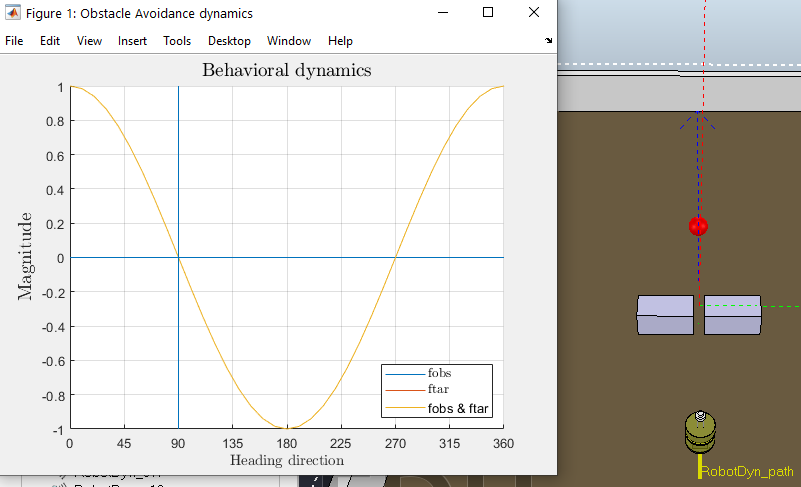
\includegraphics[width=\textwidth]{img/3-2-3-1.PNG}
    \caption{}%
    \label{fig:obs-tar-nonlinear-behavioral-10-1}
  \end{subfigure}
  % 
  \begin{subfigure}{.45\textwidth}
    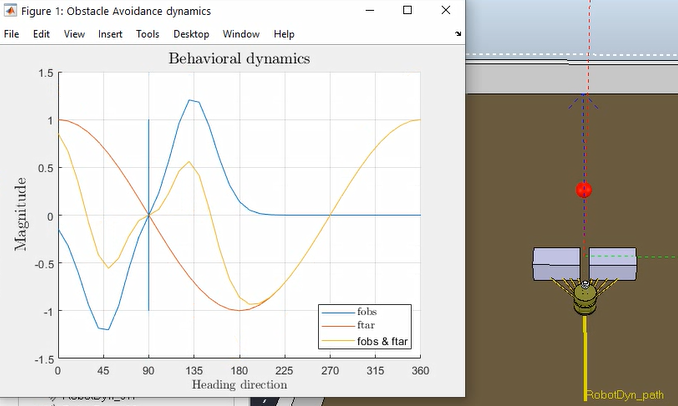
\includegraphics[width=\textwidth]{img/3-2-3-2.PNG}
    \caption{}%
    \label{fig:obs-tar-nonlinear-behavioral-10-2}
  \end{subfigure}
  % 
    \begin{subfigure}{.45\textwidth}
      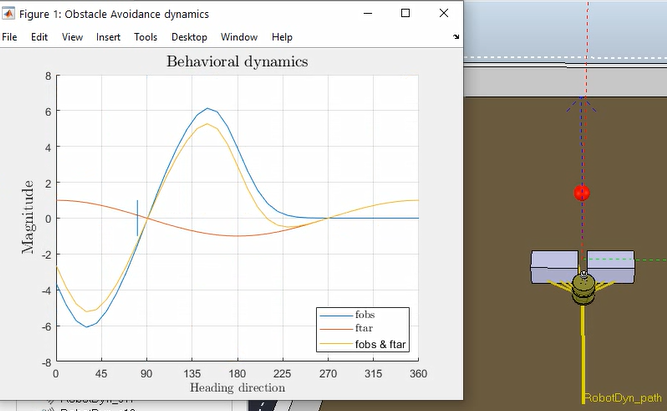
\includegraphics[width=\textwidth]{img/3-2-3-3.PNG}
    \caption{}%
    \label{fig:obs-tar-nonlinear-behavioral-10-3}
    \end{subfigure}
%
    \begin{subfigure}{.45\textwidth}
      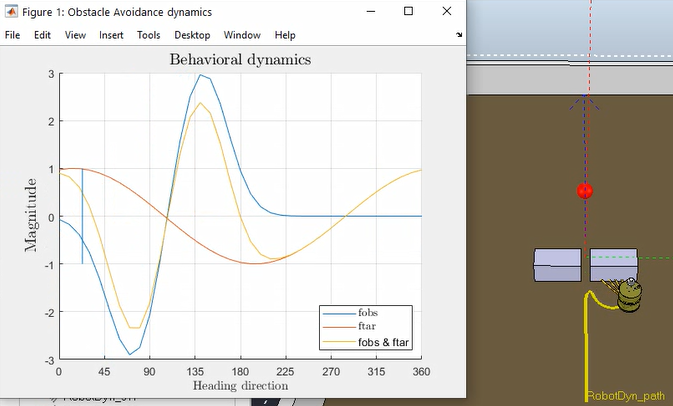
\includegraphics[width=\textwidth]{img/3-2-3-4.PNG}
    \caption{}%
    \label{fig:obs-tar-nonlinear-behavioral-10-4}
    \end{subfigure}
%
    \begin{subfigure}{.45\textwidth}
      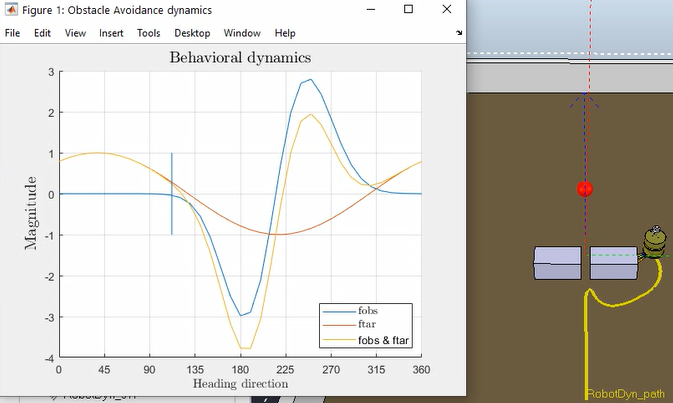
\includegraphics[width=\textwidth]{img/3-2-3-6.PNG}
    \caption{}%
    \label{fig:obs-tar-nonlinear-behavioral-10-5}
    \end{subfigure}
    % 
    \begin{subfigure}{.45\textwidth}
      \includegraphics[width=\textwidth]{img/3-2-3-7.PNG}
    \caption{}%
    \label{fig:obs-tar-nonlinear-behavioral-10-6}
    \end{subfigure}
    \caption{Behavioral Dynamics depending on the robot's position in the world for a 10 cm gap}%
    \label{fig:obs-tar-nonlinear-behavioral-10}
  \end{figure}

In Fig.~\ref{fig:obs-tar-nonlinear-behavioral-10-1} the sensors have not yet
detected obstacles, so only the target contributes to the vector field, yielding
an attractor in the forward heading direction. The robot proceeds. As the
robot approaches the obstacles, the repulsion forces present greater magnitude,
and therefore dominate, yielding a repeller in the heading direction of 90
degrees, and more, two attractors are erected, one on the left and one on the
right, giving two escape routes for the robot so that there is no collision with
the obstacles. It is in this situation that the behavior change occurs ---
the fixed point for the heading direction was asymptotically stable and now
becomes unstable, causing the robot to turn, in this case, to the
right (see Figs.~\ref{fig:obs-tar-nonlinear-behavioral-10-2} and~\ref{fig:obs-tar-nonlinear-behavioral-10-3}).

Figs.~\ref{fig:obs-tar-nonlinear-behavioral-10-4} and~\ref{fig:obs-tar-nonlinear-behavioral-10-5} show, through the diagram, that the robot progresses in the
direction of one of the attractors, and through the simulation environment, it
is seen that the robot bypasses the obstacle without collisions, because the
vector field continues with a repeller in the direction of the obstacles. With
the movement towards the attractor, the heading direction of the robot meets
the target, as desired.
%
\subsubsection{50 cm}%
\label{sec:Different-gaps-50cm}
In the last simulation, the obstacles are 50 cm apart and the robot is
positioned in front of the obstacles but without the sensors detecting them as
illustrated in Fig.~\ref{fig:obs-tar-nonlinear-behavioral-50}. 
The stochastic force is not considered and the $\beta _{2} = 50$.

\begin{figure}[htb!]
  \centering
%
  \begin{subfigure}{.45\textwidth}
  \includegraphics[width=\textwidth]{img/3-3-1.PNG}%
  \caption{}%
  \label{fig:obs-tar-nonlinear-behavioral-50-1}
  \end{subfigure}
%
  \begin{subfigure}{.45\textwidth}
    \includegraphics[width=\textwidth]{img/3-3-2.PNG}%
  \caption{}%
  \label{fig:obs-tar-nonlinear-behavioral-50-2}
  %  \caption{(b)}
  \end{subfigure}
%
  \begin{subfigure}{.45\textwidth}
    \includegraphics[width=\textwidth]{img/3-3-3.PNG}%
  \caption{}%
  \label{fig:obs-tar-nonlinear-behavioral-50-3}
  %  \caption{(c)}
  \end{subfigure}
  % 
  \begin{subfigure}{.45\textwidth}
    \includegraphics[width=\textwidth]{img/3-3-4.PNG}%
  \caption{}%
  \label{fig:obs-tar-nonlinear-behavioral-50-4}
  %  \caption{(d)}
  \end{subfigure}
%
  \begin{subfigure}{.45\textwidth}
  \includegraphics[width=\textwidth]{img/3-3-5.PNG}%
  \caption{}%
  \label{fig:obs-tar-nonlinear-behavioral-50-5}
  %\caption{(f)}
  \end{subfigure}
  \caption{Behavioral Dynamics depending on the robot's position in the world for a 50 cm gap}%
  \label{fig:obs-tar-nonlinear-behavioral-50}
\end{figure}

In the beginning (Fig.~\ref{fig:obs-tar-nonlinear-behavioral-50-1}), no obstacle
is detected --- the vector field of the dynamics of the heading direction is an attractor in the direction of the target.
As the robot continues forward, the target's contribution remains, with an
attractor in the 90-degree heading direction. In the first moments when the
robot's sensors detects obstacles (Fig.~\ref{fig:obs-tar-nonlinear-behavioral-50-2}), the sum
of its forces yields a repeller at 90 degrees, where an attractor already
exists, a contribution made by the target. It is clear by the figure that the
contribution made by the target has greater magnitude, so it dominates,
therefore in the heading direction of 90 degrees an attractor is
established. The robot proceeds forward.

With the proximity to the obstacles (Fig.~\ref{fig:obs-tar-nonlinear-behavioral-50-3}), it is increasingly noticeable that the
obstacles are spaced apart, so each contribution of the obstacles will be more
precise and, consequently, more distributed by the different degrees of heading
direction, because of this the sum of all
repulsion forces yields an attractor in the 90-degree navigation
direction. What coincides with the attractor built by the force of attraction,
the robot continues forward.

The vector field persists with this logic (Fig.~\ref{fig:obs-tar-nonlinear-behavioral-50-4}). When the robot overcomes
obstacles, the sum of these repulsive forces becomes null and insignificant for
the vector field (Fig.~\ref{fig:obs-tar-nonlinear-behavioral-50-5}).

\subsection{Influence of noise}%
\label{sec:obs-tar-nonlinear-noise}
To verify the contribution of noise, the robot was positioned at a short distance from the wall, in two episodes noise was considered (Q = 0.05 and Q = 0.5) and in another it was not taken into account (Q = 0).
It was found that in the situation in which the noise is added to the dynamics the robot manages to escape and avoid the obstacle, in the opposite situation the robot collided, illustrated in Fig.~\ref{fig:obs-tar-nonlinear-noise}.
This experiment reinforces the importance of adding noise to the dynamic system,
for when the robot is in a repeller be able to escape in a finite time. 
%
\begin{figure}[htb!]
  \centering
  \includegraphics[width=0.7\textwidth]{img/obs-tar-nonlinear-noise.PNG}
  \caption{Simulation results for the overall dynamic field with different noise levels}%
  \label{fig:obs-tar-nonlinear-noise}
\end{figure}
%

In addition, comparing the two experiments in which the noise was added it is also possible to make conclusions. The trajectory that the robot does when Q = 0.05 is smoother than when Q = 0.5. 
That said, when choosing the values of Q, it must be taken into account that the value must ensure that the robot escapes to the repeller and does not make abrupt direction adjustments, so always give preference to small values.
Since the Gaussian white noise is a stochastic function, then the trajectory
taken by the robot --- the left or right attraction basin --- will be selected
in a probabilistic way by this function, contributes for behavioral diversity
when the robot must deviate from the obstacles, enabling it to turn left or right,
depending on the stochastic effect. 
%
\subsection{Scenario 2}
In this simulation is used the \texttt{MobileRobotDyn\_Tar\_Obs\_S.ttt}
scenario, an S-shape scenario, to demonstrate the overall dynamics robustness
for a more complex scenario. As can be observed (Fig.~\ref{fig:obs-tar-nonlinear-scenario2}), the robot is able to avoid obstacles and reach the target.

\begin{figure}[htb!]
  \centering
  \includegraphics[width=0.8\textwidth]{img/mapa1.PNG}
  \caption{Simulation in the \texttt{MobileRobotDyn\_Tar\_Obs\_S.ttt} scenario}%
  \label{fig:obs-tar-nonlinear-scenario2}
\end{figure}

\subsection{Scenario 3}
In this simulation is used the \texttt{MobileRobotDyn\_Tar\_Obs\_U.ttt}
scenario, an U-shape scenario, to demonstrate the overall dynamics robustness
for an ever more complex scenario.
(see Fig.~\ref{fig:obs-tar-nonlinear-scenario3} and Video \href{run:./videos/obs-tar-nonlinear-Uscenario.mp4}{./videos/
obs-tar-nonlinear-Uscenario.mp4}). Once again, the robot is able to avoid obstacles and reach the target.
The behavior is the same as already described: in the presence of an obstacle,
a repeller is placed in that heading direction and two attractors,
representing the possible heading directions for the escape, only when these
forces are the most intense, which depends on the proximity to the
obstacle. When the sensors do not detect obstacles, only the force of attraction
to the target
contributes to the vector field of the heading direction.
%
\begin{figure}[htb!]
  \centering
  \includegraphics[width=0.7\textwidth]{img/mapa2.PNG}
  \caption{Simulation in the \texttt{MobileRobotDyn\_Tar\_Obs\_U.ttt} scenario}%
  \label{fig:obs-tar-nonlinear-scenario3}
\end{figure}

\subsection{Discussion}
In conclusion, the vector field of the navigation direction is constituted by
the attraction force and the sum of repulsion forces, with each force establishing an attractor and/or a repeller. With the movement of the robot around the world, it is expected that it will change its behavior in accordance with its surroundings. The decisions that the robot undertakes to navigate with a certain heading direction or to continue in it depends on the bifurcations.
Therefore, the stability of fixed points can change and other new fixed points
appear.

The obstacle avoidance behavior must take precedence over the target acquisition
to prevent the robot from hitting an obstacle while attempting to move to the
target. This is guaranteed by imposing greater magnitude for repulsive component than for
attractive one, i.e. $\lambda_{obs} \gg \lambda_{tar}$, and consequently,
$\tau_{obs} \ll \tau_{tar}$.

In experiments with distances between obstacles, it should be noted that the
bifurcation point slightly exceeds the diameter of the robot. This means that
the vector field has an attractor in the direction of navigation 90 degrees only
when the distance between obstacles is greater than the diameter of the robot,
otherwise it will be a repeller in this direction and two attractors for the
escape.

Finally, the stochastic force, here modelled as Gaussian white noise, is
important to ensure escape from repellers within a finite time, which would
otherwise remain in this state, provided this was the initial
condition. Additionally, noise also contributes for behavioral diversity when
the robot must deviate from the obstacles, enabling it to turn left or right,
depending on the stochastic effect. 

%%% Local Variables:
%%% mode: latex
%%% TeX-master: "../../dissertation"
%%% End:

  \setcounter{table}{0}
  \setcounter{figure}{0}
%  
  \renewcommand{\baselinestretch}{1.0}
\chapter{Integration of behaviors: Obstacle Avoidance and Target Acquisition (linear)}%
\label{ch:obstacle-target-linear}
\renewcommand{\baselinestretch}{1.5}
In this chapter the obstacle avoidance and target acquisition behaviors are
integrated, but for the latter is considered a linear dynamic system. The main
differences in the dynamics and corresponding behavior are discussed. Finally,
the best dynamic system form for target acquisition behavior --- nonlinear or linear --- is discussed.

\section{Implementation}%
\label{sec:implementation-obs-tar-linear}
The implementation of the dynamic system that controls the heading direction is
yielded by replacing the nonlinear dynamic system for target acquisition
--- $f_{tar}(\phi)$ --- for the
linear one, as given by Eq.~(\ref{eq:19}), in Eq.~(\ref{eq:36}).

\section{Simulation}
In this scenario, \texttt{MobileRobotDyn\_Tar\_Obs.ttt}, are performed two
simulations for different gaps between obstacles, namely 0 cm and 50 cm span.

\subsection{No gap (0 cm)}%
\label{sec:no-gap-linear}
In the first simulation (Fig.~\ref{fig:obs-tar-linear-behavioral}), the
obstacles form a wall and the robot is positioned in front of the
obstacles but without the sensors detecting them. 
The stochastic force is not considered and the parameter $\beta _{2}$ is 50.

In the initial moments, the sensors do not detect the wall, so the vector field
of the navigation direction is constituted by an attractor, and the dynamic is
linear, since the repulsive forces are zero and the attraction force is
linear. The 90 degrees fixed point is the attractor and there are no repellers,
the robot moves forward (Fig.~\ref{fig:obs-tar-linear-behavioral-1}).

When obstacles are detected, the repulsion forces appear and their intensity
exceeds the attraction force intensity, so in the direction of navigation 90
degrees, a repeller is established. Given the mathematical nature of the
repulsive forces, two attractors are placed, one on the right and the other on
the left, identifying the two directions of escape from the obstacle, (Fig.~\ref{fig:obs-tar-linear-behavioral-2}).

In Figs.~\ref{fig:obs-tar-linear-behavioral-3}
and~\ref{fig:obs-tar-linear-behavioral-4} the robot turns around itself, and
proceeds the navigation direction to one of the attractors, in this case, it
turns right.
The robot continues to circumvent the obstacle until the sensors stop detecting
it, so the behavior falls back to the initial one and the robot reaches the
target (Figs.~\ref{fig:obs-tar-linear-behavioral-5} and~\ref{fig:obs-tar-linear-behavioral-6}).

\begin{figure}[htb!]
  \centering
  \begin{subfigure}{.45\textwidth}
  \includegraphics[width=\textwidth]{img/4-1.PNG}%
  \caption{}%
%
  \label{fig:obs-tar-linear-behavioral-1}
  \end{subfigure}
  \begin{subfigure}{.45\textwidth}
    \includegraphics[width=\textwidth]{img/4-2.PNG}%
  \caption{}%
  \label{fig:obs-tar-linear-behavioral-2}
  \end{subfigure}
  % 
  \begin{subfigure}{.45\textwidth}
    \includegraphics[width=\textwidth]{img/4-3.PNG}%
  \caption{}%
  \label{fig:obs-tar-linear-behavioral-3}
  \end{subfigure}
  % 
  \begin{subfigure}{.45\textwidth}
    \includegraphics[width=\textwidth]{img/4-5.PNG}%
  \caption{}%
  \label{fig:obs-tar-linear-behavioral-4}
  \end{subfigure}
  \begin{subfigure}{.45\textwidth}
    \includegraphics[width=\textwidth]{img/4-6.PNG}%
  \caption{}%
  \label{fig:obs-tar-linear-behavioral-5}
  \end{subfigure}
  % 
  \begin{subfigure}{.45\textwidth}
    \includegraphics[width=\textwidth]{img/4-7.PNG}%
  \caption{}%
  \label{fig:obs-tar-linear-behavioral-6}
  \end{subfigure}
  \caption{Behavior of the linear system at no gap between obstacles.}%
  \label{fig:obs-tar-linear-behavioral}
\end{figure}

\subsection{50 cm}%
\label{sec:no-gap-linear-50}
A second experiment was carried out in the same scenario and with the same
parameters in which the robustness of both systems, linear and non-linear, were
evaluated (see Fig.~\ref{fig:obs-tar-linear-50} and Video \href{run:./videos/obs-tar-linear.mp4}{./videos/obs-tar-linear.mp4}). 
Both reached the target through the shortest path between obstacles. However,
the linear system showed more abrupt direction adjustments.

\begin{figure}[htb!]
  \centering
%
  \begin{subfigure}{.41\textwidth}
  \includegraphics[width=\textwidth]{img/linear.PNG}%
  \caption{Linear}%
  \label{fig:obs-tar-linear-50-1}%
  \end{subfigure}
%
  \begin{subfigure}{.45\textwidth}
    \includegraphics[width=\textwidth]{img/nonlinear.PNG}%
  \caption{Nonlinear}%
  \label{fig:obs-tar-linear-50-2}%
  \end{subfigure}
  % 
    \caption[Comparison of linear and nonlinear dynamic systems for target
    acquisition in the overall dynamics]{Comparison of linear and nonlinear dynamic systems for target
      acquisition in the overall dynamics at a 50cm gap between obstacles}%
    \label{fig:obs-tar-linear-50}%
\end{figure}

\section{Discussion}
After analyzing the robot's behavior for both nonlinear and linear dynamics, it
is now possible to compare them.
Mathematically, the fact that the nonlinear function is a sinusoidal function, yielding always
two fixed points --- one attractor, and in the opposite direction a
repeller --- whereas the linear function only contributes with one attractor to
the vector field. 
The repeller in the opposite direction to the target reinforces the heading direction that must be taken by the robot so that it reaches the target.
In the previous experiments, as well by Section~\ref{sec:discussion-linear-phi},
it is concluded by experimentation too, that the nonlinear system provides smoother paths at narrower angular velocity range.
Thus, it can be concluded that the nonlinear dynamic system is better for the target acquisition behavior of the robot. 

%%% Local Variables:
%%% mode: latex
%%% TeX-master: "../../dissertation"
%%% End:

  \setcounter{table}{0}
  \setcounter{figure}{0}
%  
  \chapter{Control of driving speed (Extra)}%
\label{cha:contr-driv-speed}
As aforementioned, the planning dynamics is affected by the rate of fixed points
local shifts, as the system must be able to track the attractor as it
shifts, which effectively means that it is dependent on the path velocity, $v$.
Effectively, planning dynamics attractors and repellers are established as the
robot moves through the environment and sensory information 
changes or due to environmental changes (obstacles moving in the world). To keep
the system stable, i.e. in or near an attractor at all times, the rate of such
shifts must be limited to permit the track the attractor as it shifts. One way
of accomplishing this is by controlling the path velocity of the vehicle, as the
rate of fixed points shift is determined by the relative velocity of the robot
with respect to its environment~\cite{bicho2000dynamic}.

In this chapter, a more adequate dynamic system for path velocity is established
--- enhancing overall dynamics performance --- and analysed, assessing its
performance in several scenarios.

The maximal rate of shift of the fixed points as a function of the vehicle's
velocity is given by~\cite{bicho2000dynamic}:
\begin{equation}
  \label{eq:37}
  \dot\psi_{max} \approx \frac{\Delta \psi}{\Delta t} \approx \frac{v}{d}
\end{equation}

This approximate description can be turn around to compute the desired path
velocity as a function of distance with $\gls{psi-max-dot}$ as design parameter,
that can be tuned to obtain good tracking. The desired velocity is computed
separately for each of the two constraints ($j = \{tar, obs\}$)
~\cite{bicho2000dynamic}:
\begin{equation}
  \label{eq:38}
  \gls{V-j} = \gls{d-j} \dot \psi_{max}
\end{equation}

The desired velocities are imposed through a very simple dynamics~\cite{bicho1997dynamic}:
\begin{equation}
  \label{eq:39}
  \frac{dv}{dt} = 
- c_{obs}(v - V_{obs}) \exp \Big( - \frac{(v- V_{obs})^2}{2 \sigma_v ^2}  \Big)
- c_{tar}(v - V_{tar}) \exp \Big( - \frac{(v- V_{tar})^2}{2 \sigma_v ^2}  \Big)
\end{equation}

The strengths, $\gls{c-obs}$ and $\gls{c-tar}$, are tuned such that in the presence of
strong obstacle contributions the obstacle term dominates while in the absence
of such contributions the reverse holds. A systematic way to construct a
function that indicates if obstacles contributions are present, is to integrate
force-lets, from which a potential function of the obstacle avoidance dynamics
results~\cite{bicho2000dynamic}:
\begin{equation}
  \label{eq:40}
  U(\phi) = \sum_{i = 1}^N{ \Bigg( \lambda_i \sigma_i^2  \exp \Big( - \frac{ (\phi -\psi_i)^2 }{2 \sigma_i ^2} \Big) - \lambda_i \frac{\sigma_i ^2}{\sqrt{e}}  \Bigg)  }
\end{equation}

Positive values of this potential function indicate that the heading direction
is in a repulsion zone of sufficient strenght, $\lambda_i$, so $c_{obs} > 0$ and
$c_{tar} = 0$ is required. Conversely, negative values of the potential indicate
that the heading direction is outside the repulsion range or repulsion is weak,
so now $c_{obs} = 0$ and $c_{tar} > 0$ is required~\cite{bicho2000dynamic}. 
Effectively:
\begin{equation}
  \label{eq:41}
  U(\phi) = \left\{
\begin{array}{ll}
      < 0 , & c_{obs} = 0 \wedge c_{tar} > 0 \quad \rightarrow \quad \mathrm{attractor} \\
      > 0 , & c_{obs} > 0 \wedge c_{tar} = 0 \quad \rightarrow \quad \mathrm{repeller} \\
\end{array} 
\right. 
\end{equation}

The transformation of potential levels to the strengths of the two contributions
to the velocity control makes use of a sigmoidal threshold
function~\cite{bicho2000dynamic}:
\begin{equation}
  \label{eq:42}
  \alpha(\phi) = \frac{\arctan(c U(\phi))}{\pi}
\end{equation}
ranging from $-1/2$ to $1/2$ (see Fig.~\ref{fig:lyapunov}, withdrawn from~\cite{bicho2000dynamic}). 
%
\begin{figure}[!hbt]
\centering
    \includegraphics[width=0.5\textwidth]{./img/lyapunov.png}
  \caption[Control of driving speed: threshold potential, potential and
  repulsive force-let (withdrawn from~\cite{bicho2000dynamic})]{The dashed line
    is a repulsive force-let, $f_{obs}$. Its integral provided a potential
    (solid thin line), $\gls{U}$, which is maximal near the heading direction to be
    avoided, i.e., resultant repeller. The thresholded potential (solid bold
    line), $\gls{alpha}$, serves as an indicator of those intervals of the heading
    direction from which obstacle forces repel (withdrawn from~\cite{bicho2000dynamic})}%
\label{fig:lyapunov}
\end{figure}

Finally, the following functions for
the strenghts of the two velocity contributions can be written:
\begin{equation}
  \label{eq:41}
\begin{array}{ll}
      c_{obs} = c_{v,obs} (1/2 + \alpha(\phi) ) \\
      c_{tar} = c_{v,tar} (1/2 - \alpha(\phi) ) \\
\end{array} 
\end{equation}

At sufficiently sharp sigmoids ($\gls{C}$ sufficiently large) this leads to the
required transition behavior. The parameters, $\gls{c-v-tar}$ and $\gls{c-v-obs}$,
determine the relaxation rate of the velocity dynamics in the two cases when
either the obstacle or the target constraints dominate~\cite{bicho2000dynamic}. 

The following hierarchy of relaxation rates ensures that the system relaxes to
the attractors and that obstacle avoidance has precedence over the target
contribution~\cite{bicho2000dynamic}:
\begin{equation}
  \label{eq:43}
  \lambda_{tar} \ll c_{v,tar},
  \quad
  \lambda_{obs} \ll c_{v,obs},
  \quad
  \lambda_{tar} \ll \lambda_{obs}
\end{equation}

\section{Implementation}%
\label{sec:implementation-lyapunov}
Following the guidelines presented in the previous section, the overall dynamics
with control of the driving speed was implemented. The first order differential
equation for path velocity --- Eq.~(\ref{eq:39}) --- was converted into an
algebraic recursive equation, using forward Euler's method. 

The potential function, $U(\phi)$, and thresholded potential function, $\alpha(\phi)$,
were computed as an intermediate step.
It should be noted that if no contributions from obstacles are present, then
$\alpha(\phi) = 0$, yielding both obstacles and target contributions to the path
velocity, i.e., that are two attractors for the dynamics. However, in the
beginning the initial velocity of the robot is very low, resulting in a
neglectable aceleration, thus causing the robot to move at this constant
velocity until it detects the presence of obstacles. To prevent this, if
$\alpha(\phi) = 0$, the robot moves at a reasonable constant speed.

Additionally, to assist the tuning of the parameters and the comprehension of
the overall dynamics with control of the driving speed, the potential,
$U(\phi)$, and thresholded potential ($\alpha(\phi)$) functions are plotted
alongside with the obstacle avoidance and target acquisition dynamics.

As a result, the following generic Matlab code was implemented (Listing~\ref{lst:program-dyn-obs-tar-lyapunov}):
% program_dyn_tar.m (generic)
\lstinputlisting[language=matlab, caption={Generic implementation of the overall
  dynamics with control of driving speed (not tuned)},label=lst:program-dyn-obs-tar-lyapunov,
style=custom-matlab]{./listing/program_dyn_obs_tar_lyapunov.m}%
%
\section{Simulations}%
\label{sec:sim-lyapunov}
Several simulations were performed to tune the multiple parameters and to assess
the performance of the overall planning dynamics with control of driving speed.

\subsection{Tuning}%
\label{sec:tuning-lyapunov}
The parameters were then tuned, starting from the hierarchy of relaxation rates that
ensures that the system relaxes to the attractors and that obstacle avoidance
has precedence over the target, imposed as:
%
\begin{lstlisting}[language=matlab, caption={Relaxation rates tuning},label=lst:program-dyn-lyapunov-relax-tuning,
style=custom-matlab]%

   %% obstacle
   tau_obs_min = 3.5 * dt; % flexible
   beta1 = 1/tau_obs_min; %  = lambda_obs_max = 1/tau_obs_min
   %% target
   tau_tar = 20*tau_obs_min; % relaxation time for attractor
   lambda_tar = 1/tau_tar; % attraction magnitude
   %% velocity
   c_v_obs = 10 * beta1; % obstacle contribution to velocity
   c_v_tar = 100 * lambda_tar; % target contribution to velocity

\end{lstlisting}

Next, the parameters directly related to the path velocity dynamics were tuned,
as follows:
%
\begin{lstlisting}[language=matlab, caption={Path velocity parameters tuning},label=lst:program-dyn-lyapunov-veloc-tuning,
style=custom-matlab]%

   % Lyapunov
   Rtar = 20; % target radius
   d_min = Rrobot + Rtar + 5; % minimum distance to target
   C = 100; % potential constant
   d_obs = d_min; % minimum distance to obstacle
   d_tar = d_min; % minimum distance to target
   psi_max = pi/12; % maximum rate of fixed points shift
   sigma_v = pi/6; % angular range for velocity
   Vobs = d_obs * psi_max; % maximum velocity for obstacle avoidance behavior
   Vtar = d_tar * psi_max; % maximum velocity for target acquisition behavior

\end{lstlisting}
The potential constant, $C$, was defined high enough to obtain a sharp sigmoid,
required for the transition behavior. The distance to obstacle and target were
considered as the minimum one, corresponding to the robot's size. The maximum
rate of fixed points shift,$\dot \psi_{max}$, was set to a relatively small
value, so the system can closely follow the attractors. The angular range for
velocity, $\sigma_v$, defines the range where the obstacles presence must be
accounted for path velocity dynamics,and this was set to two sensor sectors.

\subsection{S scenario}%
\label{sec:s-scenario-lyapunov}
Then, the robot's planning dynamics was simulated using the
\texttt{MobileRobotDyn\_Tar\_Obs\_S.ttt} scenario (see Fig.~\ref{fig:lyapunov-s}
and Video \href{run:./videos/lyapunov-s.mp4}{./videos/lyapunov-s.mp4}). 
%
\begin{figure}[htb!]
  \centering
%
  \begin{subfigure}{.7\textwidth}
    \includegraphics[width=\textwidth]{img/lyapunov-s-1.PNG}%
  \caption{}%
  \label{fig:lyapunov-s-1}
  \end{subfigure}
%
  \begin{subfigure}{.7\textwidth}
    \includegraphics[width=\textwidth]{img/lyapunov-s-2.PNG}%
  \caption{}%
  \label{fig:lyapunov-s-2}
  \end{subfigure} 
  % 
  \begin{subfigure}{.7\textwidth}
    \includegraphics[width=\textwidth]{img/lyapunov-s-3.PNG}%
  \caption{}%
  \label{fig:lyapunov-s-3}
  \end{subfigure}
%
  \caption{Planning dynamics with control of driving speed: Scenario S}%
  \label{fig:lyapunov-s}
\end{figure}
%
The robot moves initially with a constant, predefined, speed, with a slight tilt
due to the orientation of the target, $\psi_{tar}$. When the robot approaches
the wall, the obstacles are
detected in a significant way (Fig.~\ref{fig:lyapunov-s-1}), with the overall
dynamics establishing a repeller on the 90 degrees heading
direction. Consequently, the obstacles potential is positive in the vicinity of
the repeller, i.e. $U(\phi) > 0$, and, thus, the thresholded potential is also
positive, i.e. $\alpha(\phi) > 0$, with the defined angular range
$\sigma_v$. Hence, the robot starts to turn left --- $\phi > 90 ^{\circ}$ ---
with the path velocity defined by Eq.~(\ref{eq:39}), affected by the sigmoidal
function and the associated parameters.

Fig.~\ref{fig:lyapunov-s-2} shows a similar situation, but now the robot turns
right --- $\phi \approx -45 ^{\circ}$. Lastly, Fig.~\ref{fig:lyapunov-s-3}
illustrates the final state of the simulation when the robot reaches the target,
and only its contribution is present. There is slight mismatch between the
heading direction and the closest attractor due to the imposed path velocity
dynamics. Comparing this simulation to the nonlinear dynamics for heading
direction with linear path velocity dynamics
(Fig.~\ref{fig:obs-tar-nonlinear-scenario2}), it can be observed a more `clean'
and shortest path, although with greater cornering radius, due to the increased
average speed.

\subsection{Tar-Obs Scenario}%
\label{sec:tar-obs-scenario-lyapunov}
Then, the robot's planning dynamics was simulated using the
\texttt{MobileRobotDyn\_Tar\_Obs.ttt} scenario with a 50 cm gap between
obstacles (see Fig.~\ref{fig:lyapunov-tar-obs} and 
Video \href{run:./videos/lyapunov-tar-obs.mp4}{./videos/lyapunov-tar-obs.mp4}). 
%
\begin{figure}[htb!]
  \centering
%
  \begin{subfigure}{.49\textwidth}
    \includegraphics[width=\textwidth]{img/lyapunov-tar-obs-1.PNG}%
  \caption{}%
  \label{fig:lyapunov-tar-obs-1}
  \end{subfigure}
%
  \begin{subfigure}{.49\textwidth}
    \includegraphics[width=\textwidth]{img/lyapunov-tar-obs-2.PNG}%
  \caption{}%
  \label{fig:lyapunov-tar-obs-2}
  \end{subfigure} 
  % 
  \begin{subfigure}{.49\textwidth}
    \includegraphics[width=\textwidth]{img/lyapunov-tar-obs-3.PNG}%
  \caption{}%
  \label{fig:lyapunov-tar-obs-3}
  \end{subfigure}
  % 
  \begin{subfigure}{.49\textwidth}
    \includegraphics[width=\textwidth]{img/lyapunov-tar-obs-4.PNG}%
  \caption{}%
  \label{fig:lyapunov-tar-obs-4}
  \end{subfigure}
  % 
  \begin{subfigure}{.49\textwidth}
    \includegraphics[width=\textwidth]{img/lyapunov-tar-obs-5.PNG}%
  \caption{}%
  \label{fig:lyapunov-tar-obs-5}
  \end{subfigure}
%
  \caption{Planning dynamics with control of driving speed: Scenario Tar-Obs}%
  \label{fig:lyapunov-tar-obs}
\end{figure}

The robot moves forward, towards the target, until it starts to detect the
obstacles (Fig.~\ref{fig:lyapunov-tar-obs-1}). Although the potential function
is not null, it is negative as expected, as the target acquisition behavior is
prevalent --- an attractor is established in the heading direction. Thus, only
the target contributes to the path velocity
dynamics. Fig.~\ref{fig:lyapunov-tar-obs-2} and
Fig.~\ref{fig:lyapunov-tar-obs-3} illustrate a similar behavior, although with
slight variations in the potential function, as the robot moves in between the
obstacles. Fig.~\ref{fig:lyapunov-tar-obs-4} showcases the only brief moment
when the thresholded potential is positive, i.e. $\alpha(\phi) > 0$, as the
robot escapes the obstacles wall and the obstacle avoidance prevails over the
target acquisition behavior for the path velocity dynamics. Lastly,
Fig.~\ref{fig:lyapunov-tar-obs-5} shows the moment the robot reaches the target
with an attractor in the heading direction as expected. This simulation
showcases a critical scenario, where the robot must pass between the obstacles
at a minimum distance, yet, at a adequate velocity.
%
%
\section{Discussion}%
\label{sec:discussion-lyapunov}
The control of driving speed is critical for maintaing the stability of the
planning dynamics of the robot, as it limits the rate of fixed points shifts,
enabling the system to track the attractor as it shifts.

The shifting of fixed points for the planning dynamics can stem from robot
movement through the environment and associated sensory information 
changes or due to environmental changes (obstacles moving in the world), causing
attractors and repellers to change. To keep
the system stable, i.e. in or near an attractor at all times, the rate of such
shifts must be limited to permit the track the attractor as it shifts. One way
of accomplishing this is by controlling the path velocity of the vehicle, as the
rate of fixed points shift is determined by the relative velocity of the robot
with respect to its environment~\cite{bicho2000dynamic}.

In this chapter, a more adequate dynamic system for path velocity was
established, as the sum of obstacles and target contributions, where one of the
components dominates at all times. A systematic way to construct a
function that indicates if obstacles contributions are present, is to integrate
force-lets, from which a potential function of the obstacle avoidance dynamics
results. If the potential is positive a repeller is established for the planning
dynamics, and conversely, if negative an attractor arises. A convenient way 
to transform the potential levels to the strengths of the two contributions
to the velocity control is through the use of a sigmoidal threshold function,
defining the angular range the obstacles contribution is noticeable.

Then, the parameters were tuned considering the hierarchy of relaxation rates
--- which ensures that the system relaxes to the attractors and that obstacle
avoidance has precedence over the target --- and some rules of thumb for the
remaining path velocity parameters.

Finally, two scenarios were simulated --- S and Tar-Obs --- to assess the
performance of the overall dynamics. It was shown that, although the average
velocity was increased, the planning dynamics remains robust, suggesting a performance improvement in the overall dynamics.
%%% Local Variables:
%%% mode: latex
%%% TeX-master: "../../dissertation"
%%% End:

  \setcounter{table}{0}
  \setcounter{figure}{0}
%
%  \include{./tex/Chap/State-Art/STATE-ART}
%  \setcounter{table}{0}
%  \setcounter{figure}{0}
  %
%   %
\chapter{Theoretical foundations}
\label{cha:theor-found}
In this chapter the theoretical foundations are outlined,
providing the basic technical knowledge to undertake the project.
% 1) [X] *Project methodology: Waterfall model*
% 2) [X] *Multitasking and Pthreads*
% 3) [X] *Client-Server architecture & TCP/IP & OSI model*
% 4) [ ] /Daemons/
% 5) [ ] /Device drivers/
% 6) [ ] *Nebulizer technology for scenting*
% 7) [ ] *Gesture recognition algorithms using computer vision*
% 8) [ ] *Face detection algorithms using computer vision*
% 9) [ ] *RDBMS (Relational Database management system) (SQL)*
% 10) [ ] /User detection technologies: IR, ultrasonic/
% 11) [ ] /Camera recording and codecs/
% 12) [ ] /Image filtering APIs/
% 13) [ ] /GIFs generation/
% 14) [ ] *Social media and e-mail sharing APIs*
% 15) [ ] /UI framework: Qt/
% 16) [ ] /File transfer protocols/
% 
% Legend:
% - *Ze*
% - /Hugo/

% Proj methodology
\section{Project methodology}
\label{sec:proj-meth}
In this section the project methodologies tools are outlined, easing the
development process.

\subsection{Waterfall model}
\label{sec:waterfall-model}
For the domain-specific design of software the waterfall methodology is used.
The waterfall model (fig.~\ref{fig:waterfall}) represents the first effort to
conveniently tackle the increasing complexity in the software development
process, being credited to Royce, in 1970, the first formal description of the
model, even though he did not coin the term~\cite{sommerville1996software}. It
envisions the optimal method
as a linear sequence of phases, starting from requirement elicitation to system
testing and product shipment~\cite{cusumano1995beyond} with the process flowing
from the top to the bottom, like a cascading waterfall.

In general, the phase sequence is as follows: analysis, design, implementation,
verification and maintenance.
\begin{enumerate}
  \item Firstly, the project requirements are elicited, identifying the key
    requirements and constraints the system being developed must meet from the
    end-user perspective, captured in natural language in a product requirements document.
  \item In the analysis phase, the developer should convert the application
    level knowledge, enlisted as requirements, to the solution domain knowledge
    resulting in analysis models, schema and business rules.
  \item In the design phase, a thorough specification is written allowing the
    transition to the implementation phase, yielding the decomposition in
    subsystems and the software architecture of the system. 
  \item In the implementation stage, the system is developed, following the
    specification, resulting in the source code.
  \item Next, after system assembly and integration, a verification phase occurs
    and system tests are performed, with the systematic discovery and debugging
    of defects.
  \item Lastly, the system becomes a product and, after deployment, the
    maintenance phase start, during the product life time.
\end{enumerate}
While this cycle occurs, several transitions between multiple phases might
happen, since an incomplete specification or new knowledge about the system,
might result in the need to rethink the document.

The advantages of the waterfall model are: it is simple and easy to understand
and use and the phases do not overlap; they are completed sequentially. However,
it presents some drawbacks namely: difficulty to tackle change and high
complexity and the high amounts of risk and uncertainty. However, in the present
work, due to its simplicity, the waterfall model proves its usefulness and will
be used along the project.

As a reference in the sequence of phases and the expected outcomes from each
one, it will be used the chain of development activities and their products
depicted in fig.~\ref{fig:sw-devel-activities} (withdrawn from
\cite{bruegge2004object}).

\begin{figure}[!hbt]
\centering
    \includegraphics[width=0.6\textwidth]{./img/waterfall.png}
  \caption{Waterfall model diagram}\label{fig:waterfall}
\end{figure}

\subsection{Unified Modeling Language (UML)}
\label{subsec:uml}
To aid the software development process, a notation is required, to articulate
complex ideas succinctly and precisely. The notation chosen was the \gls{uml},
as it provides a spectrum of notations for representing different aspects of a
system and has been accepted as a standard notation in the software
industry~\cite{bruegge2004object}.

The goal of UML is to provide a standard notation that can be used by all
object- oriented methods and to select and integrate the best elements of
precursor software notations, namely \gls{omt}, Booch, and \gls{oose}
~\cite{bruegge2004object}. It provides
constructs for a broad range of systems and activities (e.g., distributed
systems, analysis, system design, deployment). System development focuses on
three different models of the system
(fig.~\ref{fig:sw-devel-activities})~\cite{bruegge2004object}:
\begin{enumerate}
  \item \textbf{\emph{The functional model}}: represented in UML with use case
    diagrams, describes the functionality of the system from the user's point of
    view.
  \item \textbf{\emph{The object model}}: represented in UML with class
    diagrams, describes the structure of the system in terms of objects,
    attributes, associations, and operations.  
  \item \textbf{\emph{The dynamic model}}: represented in UML with interaction
    diagrams, state-machine diagrams, and activity diagrams, describes the
    internal behaviour of the system.
\end{enumerate}

\begin{figure}[!hbt]
\centering
    \includegraphics[width=0.7\textwidth]{./img/sw-devel-activities.png}
  \caption{An overview of the object-oriented software engineering development
  and their products. This diagram depicts only logical dependencies among work
  products (withdrawn from~\cite{bruegge2004object})}
\label{fig:sw-devel-activities}
\end{figure}

%%% Local Variables:
%%% mode: latex
%%% TeX-master: "../../../dissertation"
%%% End:

% multitask
%
\section{Multitasking and concurrency}
\label{sec:mult-conc}
aaaaaaaa

\subsection{Pthreads}
\label{sec:pthreads}
aaaaaaaa





%%% Local Variables:
%%% mode: latex
%%% TeX-master: "../../../dissertation"
%%% End:

% cli-serv
%
\section{Communications}
\label{sec:comm}
The communications technologies and the associated tools used for the project development are briefly described next.

\subsection{IEEE 802.11 --- Wi-Fi}%
\label{sec:wifi}
IEEE 802.11, commonly known as Wi-Fi, is part of the IEEE 802 set of \gls{lan} protocols, and specifies the set of \gls{mac2} and
physical layer protocols for implementing \gls{wlan}
communication in a wide sprectrum of frequencies, ranging from 2.4--60 GHz.

\subsubsection{TCP/IP}%
\label{sec:tcpip}
The most commonly used protocols for Internet communications, including Wi-Fi,
are \gls{tcp} and \gls{ip}, usually associated together, being part of the \gls{osi} model
(Fig.~\ref{fig:osi-model}), which characterises and standardises the
communication functions of a telecommunication or computing system, being
agnostic to their underlying internal structure and technology.

A computer protocol is a standardised procedure for the exchange and
transmission of data between devices, as requested for the application processes.
The TCP provides services at the Transport layer, handling the reliable, unduplicated
and sequenced delivery of data~\cite{carne2004professional}, while the UDP provides data transportation
without guaranteed data delivery or acknowledgments. The TCP can be thought of
a reliable version of \gls{udp}, generalizing. The IP part of the TCP/IP suite, providing
services at the Network layer, is used to make origin and destination addresses
available to route data across networks.

These protocols are applied in sequence to the user's data to create a frame
that can be transmitted from the sending application to the receiving
application.
The receiver reverses the procedure to obtain the original user’s data and pass
them to the receiving application~\cite{carne2004professional}.

Another interesting fact, due to the technology agnostic aspect of the OSI
Model, is that IP and the higher-level protocols may be implemented on several
kinds of physical nets.
% OSI model
\begin{figure}[!hbt]
\centering
    \includegraphics[width=0.5\textwidth]{./img/osi-model.png}
  \caption{\gls{osi} model}%
\label{fig:osi-model}
\end{figure}
%
\subsection{Network programming --- sockets}%
\label{sec:netw-progr-sock}
Computer systems implement multiple processes which require an identifier. As
such, the IP address is not enough to uniquely identify the origin/destination
of data to be transmitted, and the port number is added. This combination of an
IP address and port number is sometimes called a network socket~\cite{wright1995tcp}, allowing
data to be delivered to multiple processes in the same machine --- same IP
address.
It is the socket pair (the 4-tuple consisting of the client IP address, client
port number, server IP address, and server port number) that specifies the two
end points that uniquely identifies each TCP connection in an
internet~\cite{wright1995tcp}. 

In a broader sense, a socket can be described as a method of \gls{ipc} that allows data to be exchanged between applications, either on
the same host (computer) or on different hosts connected by a network~\cite{kerrisk2010linux}, as a
local interface to a system, created by the applications and controlled by the
operating system, allowing an application process to simultaneously send and
receive messages from other processes.

The Socket API was created in UNIX BSD 4.1 in 1981, with widespread
implementation in UNIX BSD 4.2~\cite{kerrisk2010linux}. It implements the Client-Server paradigm and
implement several (standard) functions to access the operating system network
resources, through system calls, in Linux~\cite{kerrisk2010linux}.

There are two generic ways to use sockets: for outgoing connections --- client
socket --- and for incoming connections --- server
socket. Fig.~\ref{fig:sockets-connection} illustrates the required steps to
obtain a connected socket:
\begin{enum-c}
\item When a socket is initially created is mostly unuseful.
\item Binding the server socket associates it to an unique network tuple (address and
  port number), enabling it to be uniquely addressed.
\item When a socket server goes into listening mode, the remote devices can
  initiate the connection procedure, referring to its unique network tuple.
\item When the socket server accepts a connection, it spawns a new socket which
  is connected to the remote device, and the endpoints can effectively
  communicate. The server socket is ready to accept new incomming connections.
\end{enum-c}
% Sockets connection
\begin{figure}[!hbt]
\centering
    \includegraphics[width=0.6\textwidth]{./img/sockets-connection.png}
  \caption{Steps to obtain a connected socket (withdrawn from~\cite{huang2007bluetooth})}%
\label{fig:sockets-connection}
\end{figure}

\subsection{Client/server model}%
\label{sec:client-serv-model}
The client/server model is the most common form of network architecture used
in data communications today~\cite{hanson2000client}. A client is a system or
application that request the activity of a service provider system or
application, called servers, to accomplish specific tasks.
The client/server concept functionally divides the execution of a unit
of work between activities initiated by the end user (client) and resource responses
(services) to the activity request as a cooperative environment~\cite{hanson2000client}. The client,
typically handling user interactions and data exchange/modification in the user’s
behalf, makes a request for a service, and a server, often requiring some resource
management (synchronization and access to the resource), performs that service,
responding to the client requests with either data or status information~\cite{ibmCliServ}.

An example of a simple client-server model using the Socket \gls{api}, through system
calls, is presented in Fig.~\ref{fig:cli-serv-operation}. The operation of sockets can be explained as
follows~\cite{kerrisk2010linux}:
\begin{itemize}
\item The \texttt{socket()} system call creates a new socket, establishing the
  protocols under which they should communicate. For both client and server to
communicate, each of them must create a socket.
\item  Communication via a stream socket is analogous to a telephone call. One
application must connect its socket to another application’s socket before
communication can take place. Two sockets are connected as follows:
\begin{enumerate}
\item One application, assuming the role of server, calls \texttt{bind()} to
  bind the socket to a well-known address, and then calls \texttt{listen()} to
  notify the kernel it is ready to accept incoming connections.
\item The other application, assuming the role of client, establishes the
  connection by calling \texttt{connect()}, specifying the address of the socket
  to which the connection is to be made.
\item The server then accepts the connection using \texttt{accept()}. If the
  \texttt{accept()} is performed before the client application calls
  \texttt{connect()}, then the \texttt{accept()} blocks.
\end{enumerate}
\item Once a connection has been established, data can be transmitted in both
directions between the applications (analogous to a bidirectional telephone
conversation) until one of them closes the connection using \texttt{close()}.
\item Communication is performed using the conventional \texttt{read()} and
  \texttt{write()} system calls or via a number of socket-specific system calls
  (such as \texttt{send()} and \texttt{recv()}) that provide additional
  functionality. By default, these system calls block if the \gls{io} operation
  can’t be completed immediately. However, nonblocking \gls{io} is also
  possible.
\end{itemize}
% Overview of UNIX system calls
\begin{figure}[!hbt]
\centering
    \includegraphics[width=0.62\textwidth]{./img/cli-serv-operation.png}
  \caption{Overview of UNIX system calls with sockets implementing 
a server/client paradigm (withdrawn from~\cite{kerrisk2010linux})}%
\label{fig:cli-serv-operation}
\end{figure}

%%% Local Variables:
%%% mode: latex
%%% TeX-master: "../../../dissertation"
%%% End:

% cli-serv
\section{Daemons}
\label{sec:daemons}
In this section daemons are introduced, showing how to create them, handle
possible errors and how to communicate with them.
%
\subsection{What is a Daemon?}
A daemon is a background process that runs without user input and usually provides some service, either for the system as a whole or for user programs.~\cite{daemons-slides}

Normally, daemons are started when a system boots and, unless forcibly terminated, run until system shutdown.
Because a daemon does not have a controlling terminal, any output,
either to \textit{stderr} or \textit{stdout}, requires special handling.
They often run with \texttt{superuser privilege} because they use privileges
ports (1 - 1024) or because they have access to some sort of privileged resource.
Generally, daemons are process group leaders and session leaders, a daemon's parent is the \texttt{init} process, which has the PID of 1 (daemon is an orphan process inherited by init).

\subsection{How to create a Daemon}
The steps to create a daemon are:
%
\begin{enum-c}
\item \texttt{Fork} and exit in the parent process;
\item Create a new session in the child using the \texttt{setsid} call;
\item Make the root directory, "\texttt{/}", the child process's working directory;
\item Change the child process's umask to 0;
\item Close any unneeded file descriptor the child inherited.
\end{enum-c}

\paragraph{\textbf{Fork and exit in the parent process}}
%
A daemon is started from a shell script or the command line.
Daemons are unlike application programs because they are not interactive, i.e., they run in the background and, as a result, do not have the controlling terminal.

The parent forks and exits as the first step toward getting rid of the controlling terminal (they only need a terminal interface long enough to get started).

\lstinputlisting[language=c,firstline=1, lastline=13,
caption={},
%label=lst:kf-main-short,
style=customc]{./listing/daemon_ex.c}

\paragraph{\textbf{Create a new session in the child using the setsid call}}
%
Calling \texttt{setsid} accomplishes several things:
\begin{item-c}
%
\item It creates a new session if the calling process is not a process group leader, making the calling process the session leader of the new session;
\item It makes the calling process the process group leader of the new process group;
\item It sets the \gls{pgid} and the \gls{sid} to the \gls{pid} of the calling process;
\item It dissociates the new session from any controlling \texttt{tty}.
%
\lstinputlisting[language=c,firstline=15, lastline=20,
caption={},
%label=lst:kf-main-short,
style=customc]{./listing/daemon_ex.c}
%
\item Each process is a member of a process group, which is a collection of one or more processes generally associated with each other for the purposes of job control (\textit{\# cat ship-inventory.txt | grep booty | sort}).
\item When a new user first logs into a machine, the login process creates a new session that consists of a single process, the user’s login shell. The login shell functions as the session leader.
%
\end{item-c}

\paragraph{\textbf{Make the root directory, "/", the child process's working directory}}
%
This is necessary because any process whose current directory is on a mounted file system will prevent that file system from being unmounted.

Making "/" a daemon's working directory is a safe way to avoid this possibility.
%
\lstinputlisting[language=c,firstline=22, lastline=29,
caption={},
%label=lst:kf-main-short,
style=customc]{./listing/daemon_ex.c}
%

\paragraph{\textbf{Change the child process's umask to 0}}

This step is necessary to prevent the daemon's inherited umask from interfering with the creation of files and directories.

Consider the following scenario:
\begin{item-c}
\item A daemon inherits a umask of 055, which masks out read and execute permissions for group and other. 
\item Resetting the daemon’s umask to 0 prevents such situation.
\end{item-c}
%
\lstinputlisting[language=c,firstline=31, lastline=35,
caption={},
%label=lst:kf-main-short,
style=customc]{./listing/daemon_ex.c}
%

\paragraph{\textbf{Close any unneeded file descriptor the child inherited}}
%
This is simply a common sense step. There is no reason for a child to keep open descriptors inherited from parent.
The list of potential file descriptors to close includes at least stdin, stdout and \texttt{stderr}.
%
\lstinputlisting[language=c,firstline=37, lastline=43,
caption={},
%label=lst:kf-main-short,
style=customc]{./listing/daemon_ex.c}
%

\subsection{How to handle errors}
%
There's the \textbf{problem} that once a daemon calls \texttt{setsid}, it no longer has the controlling terminal an so it has nowhere to send output that would normally go to \texttt{stdout} or \texttt{stderr} (such as error messages).

The \textbf{solution} is that, fortunately, the standard utility for this purpose is the \texttt{syslog} service, provided by the system logging daemon, \texttt{syslogd}.

\paragraph{\textbf{Handling Errors with syslog}}
%
\texttt{syslogd} is a daemon that allow to save log messages from other daemons or applications.
The relevant interface is defined in \texttt{<syslog.h>} header file.
The \gls{api} is simple, \texttt{openlog} opens the log, \texttt{syslog} writes a message to it, and
\texttt{closelog} close the log.

The function prototypes are listed here:
%
\lstinputlisting[language=c,firstline=45, lastline=49,
caption={},
%label=lst:kf-main-short,
style=customc]{./listing/daemon_ex.c}
%

\subsection{Communicating with a Daemon}
%
To communicate with a daemon, you send a it signals that cause it to respond in a given way.
For example, it is typically necessary to force a daemon to reread its configuration file.
The most common way to do this is to send a \texttt{SIGHUP} signal to the daemon.

When you execute the command \textit{"kill PID"} on command line, the signal \texttt{SIGINT} is sent to daemon to terminate the daemon execution.

%%% Local Variables:
%%% mode: latex
%%% TeX-master: "../../../dissertation"
%%% End:

% cli-serv
%
\section{Device drivers}
\label{sec:device-drivers}
aaaaaaaa


%%% Local Variables:
%%% mode: latex
%%% TeX-master: "../../../dissertation"
%%% End:

% cli-serv
%
\section{Scenting technologies}
\label{sec:scenting-techn}
A scenting technology transforms an aromatic liquid into a gaseous fluid that
can be conveyed through the air and be captured by human olfactory sense,
usually for therapeutic or marketing purposes. As aforementioned in
Section~\ref{sec:context-motivation}, olfactory sense is the fastest way to the brain, thus, providing an exceptional
opportunity for marketing~\cite{news-harvard} --- ``75\% of the emotions we generate on a daily basis are affected by smell. Next
to sight, it is the most important sense we have''~\cite{lindstrom2006brand}.

In this section a brief overview of the scenting technologies is provided, with
special focus on ultrasonic diffusion as simple to control and cost-effective
solution.

\subsection{Overview}
\label{sec:overview}
There are several scenting technologies, mainly divided into~\cite{wen2019development}:
\begin{item-c}
\item \emph{Atomization}: it dispense odorants by transforming them into a
  gaseous fluid without requiring to heat. Its advantages are
  the dispensing process is fast and the dispensing quantity is controllable.
\item \emph{Thermalization}: it dispense odorants by vaporizing odor sources in
  the liquid state of the solid state using \gls{pwm} heaters. It requires a
  temperature controller to avoid scorching odor sources.
\item \emph{Evaporation}: it dispense odorants by conveying the liquid through a
  porous material into the outer surface (capillary action) where it evaporates
  naturally. It is a passive method, thus, not controllable.
\end{item-c}

The thermalization process requires heat which can modify fragrances, besides
requiring more power. Evaporation is a passive method, hence, not
controllable. Thus, one will focus on the \textbf{atomization} processes.

There are several atomization processes, with the most commercially relevant being~\cite{aromaUltrasonicVsNebul}:
\begin{item-c}
\item \emph{Ultrasonic diffusers}: it contains reservoirs for water and
  essential aromatic oils. It uses mechanical ultrasonic vibrations to
  brake down water molecules into droplets, producing mist, diffusing the oils
  into the air. Its advantages are: low power consumption, easy to clean,
  silent operation, and
  they double as a humidifier (can be a disadvantage too). Furthermore, they are
  a very cost-effective solution: the units themselves tend to cost less than
  nebulizing diffusers on average, but more importantly, ultrasonic diffusers
  use much less oil than nebulizing diffusers. They also run for longer periods
  of time, in several cases up to 24 hours before needing to be refilled.
  As a disadvantage they change the fragrance composition by incorporating water
  into it (this is not critical).
\item \emph{Nebulizers}:
  Nebulizing diffusers don't use water. Instead the essential oil is diffused by
  an air compressor that blows air across the top of the reservoir tube,
  creating a vacuum which pulls fine particles of the essential oil up and
  sprays them into the air around the unit. Its advantages are: fragrance
  composition is unaltered, more compact (typically), faster and more
  concentrated fragrance diffusion. The drawbacks are: less cost-effective when
  compared to ultrasonic diffusers as the oil consumption rate is much higher
  and the units are more expensive, and they tend to be noisy due to the air
  compressor operation.
\end{item-c}

The ultrasonic diffuser was preferred due to its low power consumption, silent
operation, cost-effectiveness, and easy control and assembly. The ultrasonic
diffusion process will be detailed in the following section.

\subsection{Ultrasonic diffusion}
\label{sec:ultrasonic-diffusion}
Ultrasonic diffusion uses high frequency stimuli to brake down water molecules
into droplets, producing mist, diffusing the oils into the air. The high
frequency stimuli is above 20 kHz, the upper threshold
for audible human hearing --- thus the ultrasonic naming --- and it's
accomplished using micro-mesh piezoelectric transducers.

Piezoelectric transducers are reciprocating transducers as they:
\begin{item-c}
\item respond to electric stimuli by generating mechanical displacement which,
  in turn, produces waves --- \emph{inverse-piezoelectricity}.
\item respond to mechanical displacement (applied force) by generating an
  electrical voltage signal --- \emph{piezoelectricity}.
\end{item-c}

In the present case, one is more interested in the first
phenomena. Piezoelectric transducers have a ressonant frequency, which means
they will go into a natural oscillation state, amplifying oscillations. Thus,
stimulating the piezoelectric actuator with a \gls{ac} signal at the resonant
frequency produces a strong mechanical oscillation, generating waves.
For small ressonant frequencies, the liquid, e.g. water, can easily follow the
mechanical oscillation produced.
However, when the ressonant frequency is high enough (hundreds of kHz or MHz),
the water particles cannot follow the oscillating surface, thus creating
momentary vacuum, due to the negative amplitudes, which therefore creates air
bubbles.
Then, on positive amplitudes these air bubbles are pushed across the surface,
catapulting water droplets into the air, quickly dissipating and turning into
vapor form.

Fig.~\ref{fig:piezo-transducer} illustrates a type of piezoelectric transducer
for ultrasonic diffusion --- the micro-porous mesh. It is comprised of~\cite{wen2019development}:
\begin{item-c}
\item \emph{rubber gasket}: used to isolate electric conduction from other
  conducting materials and as cushion against vibration;
\item \emph{metal substrate}: it has a micro-porous metal mesh in the center
  with a high number of trumpet-shaped cylinder micro-pores, in which the upper
  cylindrical surface is smaller than the bottom.
\item \emph{ring-shaped piezoelectric plate}: a contact is attached to the
  piezoelectric plate, so that the power wire and ground wire can be connected
  between the piezoelectric plate and the metal substrate, enabling its
  electrical stimulation.
\end{item-c}
%
\begin{figure}[htb!]
\centering
    \includegraphics[width=0.55\columnwidth]{./img/piezo-transducer.png}
  \caption{Micro-porous mesh piezoelectric transducer for ultrasonic diffusion --- withdrawn from~\cite{wen2019development}}%
\label{fig:piezo-transducer}
\end{figure}

This micro-porous piezoelectric transducer is driven by an \gls{ac} signal at a
frequency of around 113 kHz and converts electric energy into kinetic energy due
to inverse-piezoelectricity~\cite{wen2019development}. The metal substrate
vibrates along with the vibration of the ring-shaped piezoelectric plate, and
the mesh in the center of the metal substrate smashes the liquid beneath the
transducer. Some liquid flows through those micro-pores and is emitted in
micro-droplet form, due to the momentary vacuum created.

The rationale behind the micro-porous piezoelectric is due to its
versatility regarding voltage supply, small size, easy control, low power
consumption and variety of fluids that it can diffuse.
A list of micro-porous piezoelectric film properties are listed below~\cite{wen2019development}:
\begin{enum-c}
\item Diameter: 13.8 mm.
\item Low driving voltage: 3--12 V.
\item High conversion efficiency, spray volume.
\item Exit aperture is very small 4 µm.
\item Frequency: 113 kHz ± 5 kHz.
\item Capacitance: 2700 PF ± 15\%.
\item Power: 1.5--2.0 W.
\item Spray volume 30 ml/h.
\item Can atomize essential oils, perfume, water based perfumes or even mixture
  of the mentioned materials.
\item life of more than 3000 hours.
\end{enum-c}

Abid et al.~\cite{abid2015novel} proposed a novel olfactory displays' scent
dispersing module based on this type of transducer
(Fig.~\ref{fig:novel-olfactory-scent-elem}). It contains a refillable fragrance
reservoir, a cotton core and the housing for the micro-porous piezoelectric
film. The fragrance ascends to the cotton core via capillary effect,
impregnating it. When the micro-porous electric film is stimulated the fragrance
in the cotton core is diffused through the aforementioned effect.
%
\begin{figure}[htb!]
\centering
    \includegraphics[width=0.65\columnwidth]{./img/novel-olfactory-scent-elem.png}
  \caption{Micro-porous mesh piezoelectric-based scent dispense module --- withdrawn from~\cite{abid2015novel}}%
\label{fig:novel-olfactory-scent-elem}
\end{figure}

\subsubsection{Driving circuit}
\label{sec:driving-circuit}
There are several commercially available \glspl{pcb} to drive micro-porous
piezoelectric transducers. Fig.~\ref{fig:pcb-diffusion} illustrates a commercial
\gls{pcb} to drive piezoelectric transducer of 113 kHz resonance frequency.
%
\begin{figure}[htb!]
\centering
    \includegraphics[width=0.4\columnwidth]{./img/pcb-diffusion.png}
  \caption{Commercial \gls{pcb} for driving micro-porous mesh piezoelectric transducers~\cite{ebayPiezo}}%
\label{fig:pcb-diffusion}
\end{figure}

As aforementioned, piezoelectric transducers for diffusion require an \gls{ac}
signal at the resonance frequency. Fig.~\ref{fig:pcb-reverse-eng} illustrates a
possible driving circuit for these transducers. A 555-timer \gls{ic} is used in
astable mode to generate a square wave at the resonance frequency that drives a
gate of power \gls{mosfet}. This \gls{mosfet} which feeds an resonant circuit to
generate an \gls{ac} signal which stimulates the piezoelectric transducer,
producing mechanical oscillations at the resonance frequency. This application
requires a fast-switching power \gls{mosfet}, like the IRLZ44N, as the
piezoelectric transducer consumes up to 300 mA of current. 
%
\begin{figure}[htb!]
\centering
    \includegraphics[width=0.6\columnwidth]{./img/pcb-reverse-eng.png}
  \caption{Schematic of a driving circuit for micro-porous mesh piezoelectric transducers~\cite{piezoSchematic}}%
\label{fig:pcb-reverse-eng}
\end{figure}



%%% Local Variables:
%%% mode: latex
%%% TeX-master: "../../../dissertation"
%%% End:

% cli-serv
%
\section{Gesture recognition using computer vision}
\label{sec:gest-recogn-using}
aaaaaaaa


%%% Local Variables:
%%% mode: latex
%%% TeX-master: "../../../dissertation"
%%% End:

% cli-serv
%
\section{Face detection using computer vision}
\label{sec:face-detection-using}
aaaaaaaa


%%% Local Variables:
%%% mode: latex
%%% TeX-master: "../../../dissertation"
%%% End:

% cli-serv
%
\section{RDBMS}
\label{sec:rdbms}
A database is a collection of data, typically describing the activities of one
or more related organizations. For example, a university database might contain
information about the following~\cite{ramakrishnan2003database}:
\begin{item-c}
\item \emph{Entities}: such as students, faculty, courses and classrooms
\item \emph{Relationships} between entities: such as students' enrollment in
  courses, faculty teaching courses, and the use of rooms for courses.
\end{item-c}

An \acrfull{dbms} is a software designed to assist in maintaining and utilizing
large collections of data.
A \acrfull{rdbms} is a subset of \gls{dbms} with relationship between tables (entities)
and rows (entities' attributes). It follows the relational model, introduced by E.F. Codd in 1970~\cite{ramakrishnan2003database},
instead of navigational model, where in the data is stored in multiple tables.
The tables are related to each other
using primary and foreign keys. It is the most used database model widely used
by enterprises and developers for storing complex and huge amounts of
data~\cite{ramakrishnan2003database}. Some examples of \gls{rdbms} are Oracle Database,
MySQL, IBM DB2, SQLite, PostgreSQL, and MariaDB.

From the users' application standpoint, a \gls{rdbms} is a management system
for databases, but is useless unless it provides an efficient and easy method to
pose questions involving the data stored in the databases. These questions are
called queries~\cite{ramakrishnan2003database}.
A \gls{dbms} provides a
specialized language --- query language --- in which queries can be performed.
The \gls{sql} for relational databases, is now the standard.
Arguably, the most widely used form
of concurrent programming is the concurrent execution of database programs
(called transactions). Users write programs as if they are to be run by
themselves, and the responsibility for running them concurrently is given to the
\gls{dbms}~\cite{ramakrishnan2003database}.

In this section an overview is presented about \gls{rdbms} foundations:
description and storage of data in a \gls{dbms}, relational model, levels of abstraction in a \gls{dbms}, transaction management,
and the structure of a \gls{dbms}. Additionally, a brief overview over \gls{sql}
and a C++ interface is presented.

\subsection{Description and storage of data in a DBMS}
\label{sec:descr-stor-data}
The user of a \gls{dbms} is ultimately concerned about the description of
various aspects of some real-world enterprise in the form of data. There are two
important data models used~\cite{ramakrishnan2003database}:
\begin{item-c}
\item \emph{Data model}: collection of high-level data description constructs
  that hide many low-level storage details. A \gls{dbms} allows a user to define
  the data to be stored in terms of a data model, such as the \textbf{relational
  data model}. It is closer to how the \gls{dbms} stores the data.
\item \emph{Semantic data model}: more abstract, high-level data model, closer
  to human thinking, serving as an useful starting point for the database
  design. The semantic data model is subsequently translated into a database
  design in terms of the data model the \gls{dbms} actually supports.
  An example is the \emph{\acrfull{er}} model which allows the user to
  pictorially denote entities and the relationship among them. The semantic data
\end{item-c}

\subsection{Relational model}
\label{sec:relational-model}
The central data description construct in the relational model is a \emph{relation},
which can be thought as a set of
\emph{records}~\cite{ramakrishnan2003database}.
A \emph{schema} is a description of data in terms of the data model. In the
relation model, the schema for a relation specifies its name, the name of each
\emph{field} (or \emph{attribute} or \emph{column}), and the type of each
field. As an example, student information in a university database may be stored
in a relation with the following schema~\cite{ramakrishnan2003database}:
\begin{quote}
\texttt{Students(\emph{sid}: string, \emph{name}: string, \emph{login}: string, \emph{age}: integer, \emph{gpa}: real)}
\end{quote}
%
The preceding schema states that each record in the Students relation has five
fields, with field names and types as indicated. As example instance of the
student relation appears in Table~\ref{tab:relational-model-example}~\cite{ramakrishnan2003database}.
%
\begingroup
\renewcommand{\arraystretch}{0.9} % Default value: 1
\begin{table}[hbt!]
\centering
\caption{An instance of the students relation --- withdrawn from \cite{ramakrishnan2003database}}
\label{tab:relational-model-example}
\begin{tabular}{@{}lllll@{}}
\toprule
\textbf{sid} & \textbf{name} & \textbf{login} & \textbf{age} & \textbf{gpa} \\ \midrule
53666        & Jones         & jones@cs       & 18           & 3.4          \\
53688        & Smith         & smith@ee       & 18           & 3.2          \\
53650        & Smith         & smith@math     & 19           & 3.8          \\
53831        & Madayan       & madayan@music  & 11           & 1.8          \\
53932        & Guldu         & guldu@music    & 12           & 2.0          \\ \bottomrule
\end{tabular}
\end{table}
\endgroup

Each row in the Students relation is a record that describes a student,
following the schema of the Students relation. Thus, the schema can be thought
as a template for describing a student. This description can be made more
precise by specifying integrity constraints, i.e., the conditions that the
records in a relation must satisfy~\cite{ramakrishnan2003database}.
For example, one could specify that every
student had a unique \texttt{sid} value, thus making a potential candidate for a
primary key, i.e., an unique identifier that univocally identifies each record
in a relation. This information cannot be captured by simply adding another
field to the Students schema, thus requiring integrity constraints to increase
the expressiveness of the constructs of a data model~\cite{ramakrishnan2003database}.

\subsection{Levels of abstraction in a DBMS}
\label{sec:levels-abstr-dbms}
The data in a \gls{dbms} is described at three levels of abstraction, as
illustrated in Fig.~\ref{fig:dbms-abstraction-levels},
namely~\cite{ramakrishnan2003database}:
\begin{item-c}
\item \emph{External schema}: allow data access to be customized (and
  authorized) at the level of individual users or group of users.
  Any given database has exactly one conceptual schema and one
physical schema because it has just one set of stored relations, but it may have
several external schemas, each tailored to a particular group of users.
Each external schema consists of a collection of one or more views and relations
from the conceptual schema.
A \emph{view} is conceptually a relation, but the records in a view are not
stored in the DBMS. Rather, they are computed using a definition for the view,
in terms of relations stored in the DBMS.
\item \emph{Conceptual schema}: also known as the \emph{logical schema},
  describes the stored data in terms of the data model of the \gls{dbms}. In a
  \gls{rdbms}, the conceptual schema describes all relations that are stored in
  the database. The conceptual schema may be design using the \gls{er} model.
\item \emph{Physical schema}: translates how the relations described in the
  conceptual schema are actually stored on secondary storage devices such as
  disks and tapes. Decisions about the physical schema are based on the
  understanding of how the data is typically accessed, typically requiring the
  design to decide about the file organizations used to store the relations and
  to create auxiliary data structures called \emph{indexes} to speed up data
  retrieval operations.
\end{item-c}
%
\begin{figure}[htb!]
\centering
    \includegraphics[width=0.65\columnwidth]{./img/dbms-abstraction-levels.png}
  \caption{Levels of abstraction in a DBMS (withdrawn from~\cite{ramakrishnan2003database})}%
\label{fig:dbms-abstraction-levels}
\end{figure}
%
\subsection{Transaction management}
\label{sec:trans-manag}
An important task of a \gls{dbms} is to schedule concurrent accesses to data in
a safe and seamless way to the user. Such accesses are named
\emph{transactions}, i.e., any one execution of a user program in a \gls{dbms},
corresponding to the basic unit of change as seen by the \gls{dbms}. Partial
transactions are not allowed, and the effect of a group of transactions is
equivalent to some serial execution of all transactions~\cite{ramakrishnan2003database}.

For the concurrent execution of transactions to take place, a \emph{locking
  protocol} is enforced by the \gls{dbms}, establishing a set of rules to be
followed by each transaction, using a \emph{lock} --- a mechanism to control
access to database objects.
Two kinds of locks are commonly supported by a DBMS: \emph{shared locks} on an
object can be held by two different transactions at the same time, but an
\emph{exclusive lock} on an object ensures that no other transactions hold any
lock on this object~\cite{ramakrishnan2003database}.

Transactions can be interrupted before running to completion for a variety of
reasons, e.g., a system crash. A DBMS must ensure that the changes made by such
incomplete transactions are removed from the database. To do so, the DBMS
maintains a log of all writes to the database, even before
the corresponding change is reflected in the database itself, enabling the
\gls{dbms} to detect and undo the changes if a system crash occurs. This property is called \gls{wal}. To ensure this property, the
DBMS must be able to selectively force a page in memory to disk~\cite{ramakrishnan2003database}.

The log is also used to ensure that the changes made by a successfully completed
transaction are not lost due to a system crash, as explained. Bringing
the database to a consistent state after a system crash can be a slow process,
since the DBMS must ensure that the effects of all transactions that completed
prior to the crash are restored, and that the effects of incomplete transactions
are undone. The time required to recover from a crash can be reduced by
periodically forcing some information to disk; this periodic operation is called a \emph{checkpoint}~\cite{ramakrishnan2003database}.

Summarizing, the main takeaways for \gls{dbms} support for concurrency control
and recovery are~\cite{ramakrishnan2003database}:
\begin{item-c}
\item \emph{Locking}:
every object that is read or written by a transaction is first locked in shared
or exclusive mode, respectively. Placing a lock on an object restricts its
availability to other transactions and thereby affects performance.
\item \emph{\gls{wal}}: for efficient log maintenance, the DBMS must be able to
  selectively force a collection of pages in main memory to disk. \gls{os}
  support for this operation is not always satisfactory.
\item \emph{Periodic checkpoint}:
  can reduce the time needed to recover from a crash. There is a trade-off
  between speed and system integrity, as checkpointing too often slows
  down normal execution. 
\end{item-c}
%
\subsection{Structure of a RDBMS}
\label{sec:structure-rdbms}

Fig.~\ref{fig:dbms-abstraction-levels} shows the structure (with some
simplification) of a typical \gls{dbms} based on the relational data model.
%
\begin{figure}[htb!]
\centering
    \includegraphics[width=0.75\columnwidth]{./img/dbms-struct.png}
  \caption{Architecure of a DBMS (withdrawn from~\cite{ramakrishnan2003database})}%
\label{fig:dbms-abstraction-levels}
\end{figure}
%

It is comprised of~\cite{ramakrishnan2003database}: 
\begin{item-c}
\item \emph{Interfaces}:
  The DBMS accepts \gls{sql} commands generated from a
  variety of user interfaces, produces query evaluation plans, executes these
  plans against the database, and returns the answers. SQL commands can also be
  embedded in host-language application programs, e.g., Java or C++ programs,
  but here one concentrates only on the core DBMS functionality.
\item \emph{\gls{dbms}}: contains:
  \begin{itemize}
  \item \emph{Query Evaluation Engine}:
    When a user issues a query, the parsed query is presented to a query
    optimizer, which uses information about how the data is stored to produce an
    efficient execution plan for evaluating the query. An execution plan is a
    blueprint for evaluating a query, and is usually represented as a tree of
    relational operators (with annotations that contain additional detailed
    information about which access methods to use, etc.).
  \item \emph{Concurrency control}:
  The \emph{Transaction Manager} ensures that transactions request and release
  locks according to a suitable locking protocol and schedules the execution
  transactions.
%
  The \emph{Lock Manager} keeps tracks of request for locks and grants locks on
  database objects when they become available.
 % 
  \item \emph{Recovery manager}:
    responsible for maintaining a log, and restoring the system to a consistent
    state after a crash.
  \item \emph{Disk access manager}:
    The \emph{file and access methods} layer includes a variety of software for
    supporting the concept of a file, which, in a DBMS, is a collection of pages
    or a collection of records. This layer typically supports a heap file, or
    file of unordered pages, as well as indexes.
    In addition to keeping track of the pages in a file, this layer organizes
    the information within a page.
%
    The \emph{Buffer manager} handles pages as a response to read requests.
%   
    The \emph{disk space manager} deals with management of space on
    disk, where the data is stored. Higher layers allocate, deallocate, read,
    and write pages through (routines provided by) this layer.
  \end{itemize}
\item \emph{Database}: contains the system catalog information consisting of the
  index files referencing the data files storing the actual data on physical
  memory.
\end{item-c}

\subsection{Database design overview}
\label{sec:datab-design-overv}
%
The database design process can be divided into six steps, namely~\cite{ramakrishnan2003database}:
\begin{enum-c}
\item \emph{Requirements Analysis}:
  the requirements for the database
  application are elicited and analyzed assessing what data is to be stored in
  the database, what applications must be built on top of it, and what operations are most frequent and subject to performance
  requirements.
Several methodologies have been proposed for organizing and presenting the
information gathered in this step, and some automated tools have been developed
to support this process.
\item \emph{Conceptual Database Design}:
the information gathered in the previous step is used to develop a high-level
description of the data to be stored in the database, along with the constraints that are known to hold over this data. This
step is often carried out using the \gls{er} model, or a similar high-level data model.
\item \emph{Logical Database Design}:
  A DBMS must be chosen to implement the database
design, and convert the conceptual database design -- \gls{er} schema --- into a database schema in the
data model of the chosen DBMS --- relational schema.
\item \emph{Schema Refinement}:
  Next, the collection of relations in the relation database schema are analyzed
  to identify potential problems, and to refine it. This is performed by
  normalizing relations, restructuring them to ensure some desirable
  properties.
\item \emph{Physical Database Design}:
  In this step, the typical expected workloads that the database must support
  are analyzed and further refine the database design to ensure that it meets
  desired performance criteria. This may simply involve building indexes on some tables and clustering some tables, or it may involve a substantial
  redesign of parts of the database schema obtained from the earlier design steps.
\item \emph{Security Design}:
  Lastly, the different user groups and different
roles played by various users are identified (e.g., the development team for a
product, the customer support representatives, the product manager).
For each role and user group, the permitted and forbidden parts of the database
are identified and the policies are enforced to ensure this. A DBMS provides
several mechanisms to assist in this step.
\end{enum-c}
%
\subsection{Entity-Relationship model}
\label{sec:entity-relat-model}
%
The \acrfull{er} data model enables the description of the data involved in a
real-world enterprise in terms of entities and their relationships and is widely
used to develop an initial database design. The \gls{er} model is most relevant
to the first three steps of the database
design~\cite{ramakrishnan2003database}~(see Section~\ref{sec:datab-design-overv}).
In this section are presented the
key concepts for the \gls{er} model as a database design modeling tool.
%

\subsubsection{Key concepts}
\label{sec:key-concepts}
It is important to understand some key concepts for the \gls{er} model, namely~\cite{ramakrishnan2003database}:
\begin{item-c}
\item \emph{Entity}: is an object in the real world that is distinguishable from
  other objects, e.g., the Pokemon toy, the toy department, the manager of the
  toy department, etc.
\item \emph{Entity set}: collection of entities. They do not need to be
  disjoint, i.e., entities can simultaneously belong to different entity
  sets. For example, one can define an entity set called \texttt{Employees} that
  contain both the toy and appliance department employee sets.
  An entity set is represented by a rectangle in the \gls{er} model.
\item \emph{Attributes}: an entity is described using a set of attributes. All
  entities in a given entity set have the same attributes. For example, the
  \texttt{Employees} entity set could use \texttt{name}, social security number
  (\texttt{ssn}) and parking lot (\texttt{lot}) as attributes.
  An attribute is represented by an oval in the \gls{er} model.
\item \emph{Domain}: for each attribute associated with a set, one must identify
  a domain of possible values. For example, the domain associated with the
  attribute \texttt{name} of \texttt{Employees} might be the set of 20-character
  strings.
  The domain information can be listed along the attribute name.
\item \emph{Key}: minimal set of attributes whose values uniquely identify an
  entity in the set. There could be more than one \emph{candidate} key: if so,
  one designate one of them as the \emph{primary} key.
  Each attribute in the primary key is underlined in the \gls{er} model. The
  \emph{foreign key} is(are) the
  attribute(s) which in a relationship one-to-many is(are) primary key(s) in the
  entity of the side \texttt{one} and integrates the set of attributes of the
  entity in the side \texttt{many} of that relationship
\item \emph{Relationship}: association between two or more entities.
  For example, one may have the relationship that Joe works in the pharmacy
  department.
  A relationship is represented by a straight line in the \gls{er} model and may
  also have \emph{descriptive attributes}.
\item \emph{Relationship set}: collection of similar relationships.
\item \emph{Key constraints}: restrictions over entities.
  For example, the restriction that each department has at most one manager, and
  is denoted by using an arrow from the entity to the relationship.
\item \emph{Participation constraints}: states the participation of an entity
  set in the relationship. It can be \emph{partial} or \emph{total}.
  For example, if every department is required to have a manager, the
  participation of the entity set \texttt{Departments} in the relationship set
  \texttt{Manages} is said to be \emph{total}.
\item \emph{Class hierarchies}: classification of entities in an entity set into
  subclasses, using the relationship \emph{is a}. For example, a \texttt{Car}
  \texttt{is a} \texttt{Vehicle} and a \texttt{Truck} \texttt{is a}
  \texttt{Vehicle} too. 
\item \emph{Aggregation}: indicates that a relationship set (identified through
  a dashed box) participates in another relationship set.
\end{item-c}

The \glspl{erd} use a graphical conventional to quickly and clearly depict the
entities involved and how they relate to each other. In a \gls{erd} entities are
represented by rectangles, attributes by ellipses, and the relationships as
lines between entities. In the rectangles and ellipses are placed the names of
the different entities and attributes. The relationships have cardinalities --- \texttt{1:1}
(one-to-one), \texttt{1:M} (one-to-many), and \texttt{M:N} (many-to-many) ---
and may be mandatory or optional --- e.g., a vehicle may not have any parking
space assigned, but to each parking space is assigned one, and one only,
vehicle.

Several notations can be used, namely, crow's foot, \gls{uml}, Chen, Barker,
etc~\cite{crowsfootNotation}.
In crow's foot notation:
\begin{item-c}
\item A multiplicity of one and a mandatory relationship is represented by a
  straight line perpendicular to the relationship line.
\item A multiplicity of many is represented by the three-pronged `crow-foot'
  symbol.
\item An optional relationship is represented by an empty circle.
\end{item-c}

Fig.~\ref{fig:erd-example} illustrates an example of an \acrfull{erd} using
crow's foot notation for an a company. There are three entity sets ---
\texttt{Customers}, \texttt{Orders}, and \texttt{Shipments}. Within each of
these are the attributes, with the primary key being underlined. Additionally it
also indicates the foreign key that resolves the \texttt{one-to-many}
relationship. Thus, a customer can place \texttt{0} or \texttt{many} orders, which, in
turn, can have \texttt{0} or \texttt{many} shipment methods.

%
\begin{figure}[htb!]
\centering
    \includegraphics[width=0.8\columnwidth]{./img/erd-example.png}
  \caption{Example of an \gls{erd}}%
\label{fig:erd-example}
\end{figure}
%




\subsection{Choice of the RDBMS}
\label{sec:choice-rdbms}
In this section are presented the most relevant \glspl{rdbms}, focusing
specially on the open-source (and free) systems, namely \texttt{MySQL} and
\texttt{SQLite}.

The most relevant \glspl{rdbms} are~\cite{modernDBChoice}:
% src: https://www.xplenty.com/blog/which-database/
\begin{item-c}
\item \textbf{Oracle Database}: 
Oracle has provided high-quality database solutions since the 1970s. The most
recent version of Oracle Database was designed to integrate with cloud-based
systems, and it allows you to manage massive databases with billions of
records.
    \begin{itemize}
    \item \emph{Advantages}: the most advanced technology and a wide range of
    solutions.
    \item \emph{Disadvantages}: an expensive solution and system upgrades might be
    required ---  many businesses have to upgrade their hardware before using Oracle
    solutions.
    \item \emph{Best use case}: if you're a large organization that needs to manage
    a massive amount of data, Oracle could be the ideal choice.
  \end{itemize}
\item \textbf{Microsoft SQL Server}: it is a database engine that is compatible
  with, both, on-site and cloud-based servers, and supports Windows and Linux
  OSes.
    \begin{itemize}
    \item \emph{Advantages}: it is mobile: this database engine allows you to
      access dashboard graphics and visuals via mobile devices. It integrates
      with Microsoft products.  It is fast and stable.
    \item \emph{Disadvantages}: an expensive solution and requires a lot of
      \gls{hw} resources.
    \item \emph{Best use case}: if you're an enterprise-level corporation that
      relies heavily on Microsoft products, the speed, agility, and reliability
      of Microsoft SQL Server could be an excellent choice.
  \end{itemize}
\item \textbf{MySQL}: MySQL is a free, open-source RDBMS solution that Oracle
  owns and manages. Even though it's freeware, MySQL benefits from frequent
  security and features updates. Large enterprises can upgrade to paid versions of MySQL to benefit from additional features and user support.
    \begin{itemize}
    \item \emph{Advantages}: it is open-source, free of charge (freeware) and
      highly compatible with many other database systems.
    \item \emph{Disadvantages}: lacking features common to other \glspl{rdbms}:
      because MySQL prioritizes speed and agility over features, some of the
      standard features found in other solutions may be missing, e.g., the
      ability to create incremental backups. Challenges getting quality support:
      The free version of MySQL does not come with on-demand support. However,
      MySQL does have an active volunteer community, useful forums, and a lot of
      documentation.
    \item \emph{Best use case}: MySQL is a particularly valuable RDBMS solution
      for businesses that need a solution with enterprise-level capabilities,
      but are operating under strict budget constraints. It is an extremely
      powerful and reliable modern RDBMS with a free tier.
  \end{itemize}
\item \textbf{SQLite}:
\end{item-c}

\subsection{SQL}
\label{sec:sql}
Ideally, a database language allows the creation of a database and table
structures, the execution of basic data management tasks (add, delete, and
modify), and the execution of complex queries designed to transform the raw data
into useful information. Moreover, it must provide a clear and easy suntax, it
must be portable and conform to some basic standard. \gls{sql} complies well to
these requirements~\cite{coronel2016database}.

\gls{sql} functions fit into two broad categories~\cite{coronel2016database}:
\begin{enum-c}
\item It is a \emph{\gls{ddl}}: SQL includes commands to create database objects
  such as tables, indexes, and views, as well as commands to define access
  rights to those database objects (see Fig.~\ref{fig:sql-dll}).
\item It is a \emph{\gls{dml}}: SQL includes commands to insert, update, delete,
  and retrieve data within the database tables (see Fig.~\ref{fig:sql-dml}).
\end{enum-c}
%
\begin{figure}[htb!]
\centering
    \includegraphics[width=0.9\columnwidth]{./img/sql-dll.png}
  \caption{SQL data definition commands --- withdrawn from~\cite{coronel2016database}}%
  \label{fig:sql-dll}
\end{figure}
%
\begin{figure}[htb!]
  \centering
  % 
  \begin{subfigure}[t]{.9\textwidth}
  \includegraphics[width=\textwidth]{img/sql-dml-1.png}%
  %\caption{main}%
  %\label{fig:state-mach-local-superv-main}
\end{subfigure}
%
%\vspace{-0.1\textwidth}
%
  \begin{subfigure}{.9\textwidth}
  \includegraphics[width=\textwidth]{img/sql-dml-2.png}%
  %\caption{Mode Manager}%
  %\label{fig:state-mach-local-superv-mode}
\end{subfigure}
  % 
  \caption{SQL data manipulation commands --- withdrawn from~\cite{coronel2016database}}%
  \label{fig:sql-dml}
\end{figure}
%


\subsection{SQL C++ interface}
\label{sec:sql-c++-interface}





%% Local Variables:
%% mode: latex
%% TeX-master: "../../../dissertation"
%% End:

% cli-serv
%
\section{Motion detection}
\label{sec:motion-detection}
The \texttt{\gls{mdo-l}} needs to be capable of detecting a user, in order to switch between \texttt{normal mode} to \texttt{interaction mode}.
In order to do such thing, it is mandatory to have a system that detects the motion of a user that approaches to the local system \texttt{\gls{mdo-l}}.

\subsection{Different types of detection}
There are several ways to do motion detection, through different sensors, such as~\cite{sensors-list}:
%
\begin{itemize}
\item \emph{\gls{pir}}: A passive infrared sensor detects body heat (infrared energy) by looking for changes in temperatures. 
This is the most-widely-used motion sensor in home security systems~\cite{sensors-list}.

Once the PIR motion sensor warms up, it can detect heat and movement in the surrounding areas, creating a protective "grid".
If a moving object blocks too many grid zones and the infrared energy levels change rapidly, the infrared sensor triggers an alarm~\cite{sensors-list}.
%
\item \emph{\gls{mw}}: This type of sensor sends out microwave pulses and measures the reflections off of moving objects.
They cover a larger area than infrared sensors but are more expensive and vulnerable to electrical interference~\cite{sensors-list}.
%
\item \emph{Dual technology motion sensors}: Some motion sensors can combine multiple detection methods in an attempt to reduce false alarms.
For example, it's not uncommon for a dual technology sensor to combine a \gls{pir} sensor with a \gls{mw} sensor~\cite{sensors-list}.
%
\item Less common types of motion detectors:
	\begin{item-c}
	\item \emph{Area reflective sensors}: This kind of sensors emit infrared rays from an LED and use the reflection of those rays to measure the distance to the person or object, allowing for detection when the subject moves within the designated area~\cite{sensors-list}.
	%
	\item \emph{Ultrasonic motion sensors}: This sensors measure the reflections off of moving objects via pulses of ultrasonic waves~\cite{sensors-list}.
	%	
	\item \emph{Vibration motion sensors}: This type of sensors detect small vibrations that people cause when they move through a room~\cite{sensors-list}.
	\end{item-c}
	%
\item Specialized motion sensors:
	\begin{item-c}
	\item \emph{Contact sensors}: Contact sensors use a magnet to spot movement on a door or window. When the sensor and corresponding magnet move apart as a door or window opens, the sensor triggers~\cite{sensors-list}.
	%
	\item \emph{Pet-immune motion sensors}: Most passive infrared sensors can ignore animals up to a certain weight. A dual technology motion sensor is more pet resistant to false alarms because it requires two sensors to be triggered a certain way~\cite{sensors-list}. 
	%	
	\end{item-c}
\end{itemize}

\subsection{Trade-off between sensors}
As it can be seen previously, there are several types of sensors that can be used. However, it is mandatory to make a trade-off between each type in order to choose the better case, according several factors such as price, range, applicability, conditions of use and others.

For this specific case, it is necessary a set of sensors with a low range detection (more or less than 1,5 meters), a good reflection and low consumption. Thus, the type of sensors that match all these criteria are ultrasonic sensors.
The reasons to discard the others sensors are simple:

Firstly, the \gls{pir} sensor actuates with changes in radiation, which means that some other case can occur where is not a human approaching the \gls{mdo-l} like, for example, an animal.

In second place, the Infrared Reflective sensors have too specific characteristics of behavior. 
For example, there are some surfaces that do not reflect quite good the \gls{ir} radiation, which could easily result on a bad behavior for two different users.

Lastly, the contact sensors are out of question for obvious reasons: there is no need to have a contact between the \gls{mdo-l} and an user.

Concluding, the best option is to use a set of ultrasonic sensors, in order to avoid some specific situations and make the user detection as better as possible.

\subsection{Ultrasonic sensor}
Ultrasonic sensors work by sending out a sound wave at a frequency above the range of human hearing.
Ultrasonic waves are sound waves emitted at a frequency higher than can be detected by human hearing — typically above 20 kHz~\cite{ultrasonic-sensor-img}.

As it can be seen in Fig.~\ref{fig:ultrasonic-sensor}, many ultrasonic sensors use a single transducer to send a pulse and to receive the echo, others use one transducer to send the pulse and another to receive it.  
The sensor determines the distance to a target by measuring time lapses between the sending and receiving of the ultrasonic pulse~\cite{ultrasonic-sensor}.

\begin{figure}[!hbt]
\centering
    \includegraphics[width=0.6\textwidth]{./img/ultrasonic-sensor.png}
  \caption{Example of the behaviour of an ultrasonic sensor(withdrawn from~\cite{ultrasonic-sensor-img})}%
\label{fig:ultrasonic-sensor}
\end{figure}

%%% Local Variables:
%%% mode: latex
%%% TeX-master: "../../../dissertation"
%%% End:

% cli-serv
%
\section{Camera recording and codecs}
\label{sec:camera-record-codecs}

In this project's local system (\gls{mdo-l}), the \texttt{Interaction Mode} is composed by an interaction made through video between the machine and the user.
To make possible that interaction through video, it is necessary to know how to record and show the frames captured by the camera using the Raspberry Pi. 

The process of recording is just simply capture several frames in a specific period and then when all frames are joined together it creates a video.
The more frames are captured per second, the more fluid the video becomes, that's why it is normal to talk about \gls{fps} when talking about video recording or playing.

\subsection{Camera recording}
\label{sub-sec:camera-record}
It is possible to capture video from the raspberry using its camera module (V2) with the help of the \texttt{OpenCV} library.
With a simple code in C++, it is possible to capture frames and show them in loop, in order to always refresh what the camera is recording.
Listing \ref{lst:camera-example} implements how to show what is being captured by the camera. Basically it is created a variable \texttt{frame} to read the frames of the camera and the \texttt{cap} refers to the camera (which in this case has 0 that represents the camera ID).
Then, basically it is just needed to verify if the camera is opened and if so read the frame from the camera and show it. This last two steps are executed in a infinite loop until a key is pressed to stop the execution. 
%
\lstinputlisting[language=C++,firstline=1,
caption={Example of camera frames acquisition (withdrawn from \cite{camera-example})},
label=lst:camera-example,
style=custom-cpp]{./listing/camera-example.cpp}

\subsection{Video files encoding (codecs) and formats}
\label{sub-sec:codecs-and-formats}
Video encoding formats, also called video file formats, are methods of optimizing digital video files for different platforms, programs, and devices.
There are many different kinds of video encoding formats, but each is composed of two main parts: a \texttt{codec} and a \texttt{container}~\cite{video-encoding}. But firstly, it is necessary to know how video encoding works.

Video encoding is the process of turning uncompressed video input into a form that can be stored and played by a variety of devices and thisi envolves two main processes: \texttt{compression} and \texttt{transcoding}~\cite{video-encoding}.
%
\begin{item-c}
\item \emph{Compression}: decreases the size of a video file so that it is more manageable. Without proper compression, most files would be far too large to upload easily, load quickly, or play smoothly on users' devices.
\item \emph{Transcoding}: refers to the total audio and video conversion process from one video format to another. It ensures that a video file is compatible with the video player and/or platform it is using. Without transcoding, users would not be able to watch the video file at all.
\end{item-c}

On-demand streaming video is encoded so that it can be sent over the Internet and played on a variety of user devices. During live streaming, the video stream is segmented, compressed, and encoded in real time~\cite{video-encoding}.

\subsubsection{What is a codec?}
A codec (coder/decoder) is a method for compressing and decompressing data so that it can be easily transported and received by different applications. Separate codecs are used to compress audio and video files, but they generally work in the same way~\cite{video-encoding}.
Codecs encode files using either lossy compression or lossless compression. Lossy compression simplifies the data in a video file and only keeps the essential parts. This is why a video using lossy compression may look pixelated or "fuzzy"~\cite{video-encoding}. 

\subsubsection{What is a container?}
A container combines an encoded audio stream (audio codec), encoded video stream (video codec), and metadata in a single video file. The metadata tells the video player how to coordinate different audio and video codecs and may also provide additional elements, such as subtitles or alternate audio streams~\cite{video-encoding}.
Each container supports a different range of video codecs. Some containers only work with a single type of codec and video player, which drastically limits playback options. Other containers are compatible with many types of video codecs and players~\cite{video-encoding}.

\subsubsection{Most common types of video formats}
There are many types of video encoding formats and they are not compatible with the same platforms, browsers and devices.
These are the most common video formats~\cite{video-encoding}:
\begin{item-c}
\item \emph{MP4}: is a video file format created by the Motion Picture Expert Group. It compresses audio and video separately, which allows MP4 files to retain relatively high video quality after compression. Most browsers and iOS/Android devices are compatible with MP4 files.
%
\item \emph{MOV}: is a video file format created by Apple. Although it can run on both Mac OS and Windows OS, it is only compatible with QuickTime video players. It preserves video quality, but does not offer as much file compression as other common video formats, such as MP4.
%
\item \emph{AVI}: is a video file format created by Microsoft. It is one of the oldest video file container specifications. AVI works with a number of different codecs, which can affect how well it is supported by different operating systems and browsers. It prioritizes video quality over compression, meaning that video files are larger and better quality overall.
%
\item \emph{FLV}: is a video file format created by Adobe Flash. A clear advantage of FLV is its ability to compress video files without severe loss of video quality. However, it is far less compatible across devices and OSes than other file formats: Though it is supported by most browsers and Android devices, it cannot be used to play any video files on iOS devices like iPhones or iPads. Browsers have dropped support for Adobe Flash because it is considered to be insecure, and Adobe no longer supports Flash.
%
\item \emph{WebM}: is a video file format developed by Google. It is a subset of the open-standard Matroska Video Container (MKV) format, which is highly adaptive to most video and audio codecs and compatible with a wide range of platforms and devices. WebM is a web-friendly, open-source alternative to MP4 that maintains high video quality after compression.
\end{item-c}

\subsection{Video players for Raspberry Pi}
\label{sub-sec:video-player}
It is necessary to have a video player in the Raspberry Pi, in order to play the video that are encoded.
The more extendable the player is, the more easier and practical it is to use.
There are two main video players that can be used on Raspberry~\cite{video-player-rasp}:
%
\begin{item-c}
\item \emph{VLC}: is one of the best video players that one can install on the Raspberry Pi. It will play almost any video and audio format that one throws at it. This means that it's not needed to spend time finding particular codecs to get videos or music playing on Raspberry Pi.
\item \emph{OMXPlayer}: is a video player for the Raspberry Pi that can run completely from the terminal. This video player has been heavily optimized for the Raspberry Pi's hardware and was designed originally as a testbed for the Kodi media player. While OMXPlayer does not have as a wide range of support as VLC, it still has its uses for those who don't want a full-blown video player.
\end{item-c}

In conclusion, for this project the best video player that can be used is the \texttt{OMXPlayer} for its capability of running completely in the terminal, which can be a very useful feature in several cases such as testing through the \texttt{Admin Remote Client} the operation of the \gls{mdo-l}.

\subsection{Playing video in C++}
\label{sub-sec:play-video-cpp}
Although there's already a solution to play videos through terminal, it is also necessary to play videos in the \gls{ui} and for that case it is mandatory to have a library that can do video playback.

One library that is very useful to do playback is the \texttt{OpenCV} library, having the advantage that this is already used in other subsystems of the project.
This library has also the advantage of working compatibly with the chosen \texttt{ui} (explained later on section \ref{sec:ui-framework}). 

\subsubsection{Example of video playback}
Here's an example on how to play a video using this library in C++:

Firstly, the definition of the \texttt{Player()} class that handles the video playback.
Listing \ref{lst:video-play-cpp-class} shows the \texttt{Player()} class that needs the \texttt{frame} to do the acquisition of the frames of the video, the \texttt{frameRate} to know the video frame rate and the \texttt{img} that is used to show the frame.
%
\lstinputlisting[language=C++,firstline=1,
caption={Example of video playback in OpenCV uisng C++ - Player class (withdrawn from \cite{video-play-cpp})},
label=lst:video-play-cpp-class,
style=custom-cpp]{./listing/video-play-class.cpp}
%
Then, listing \ref{lst:video-play-cpp} shows the implementation of the main member functions.
Firstly, the \texttt{loadVideo} function loads the video and reads the framerate of the video.
Then, the \texttt{run} function reads the frame from the video, attributes it to the \texttt{img} to be then showed on the widget and finally waits the specific time to show the next frame in order to respect the video's frame rate, all this execution occurs while the video doesn't stop.
Lastly, the \texttt{updatePlayerUI} puts the image on the widget using the functions that \texttt{Qt} already gives.
%
\lstinputlisting[language=C++,firstline=1,
caption={Example of video playback in OpenCV uisng C++ - Player class implementation(withdrawn from \cite{video-play-cpp})},
label=lst:video-play-cpp,
style=custom-cpp]{./listing/video-play.cpp}
%%% Local Variables:
%%% mode: latex
%%% TeX-master: "../../../dissertation"
%%% End:

% cli-serv
%
\section{Image filtering}
\label{sec:image-filtering}
aaaaaaaa


%%% Local Variables:
%%% mode: latex
%%% TeX-master: "../../../dissertation"
%%% End:

% cli-serv
%
\section{GIF generation}
\label{sec:gif-generation}
aaaaaaaa


%%% Local Variables:
%%% mode: latex
%%% TeX-master: "../../../dissertation"
%%% End:

% cli-serv
\section{Social media sharing APIs}
\label{sec:social-media-sharing}
Social media platforms are great contact points to target customers and to
increase brand awareness, which is highly desirable for digital marketing. These
platforms provide a set of functionalities to external agents interact with them
in a programmatic way, enabling automation of tasks like content sharing,
scheduling, search, etc.
These functionalities are exposed by \glspl{api}, providing a custom and
well-defined interface that can be explored by developers to build custom
applications that leverages on them.

There are several social media platforms, but here one focuses on the most
popular ones, namely~\cite{rakutenTop10SMApis, ayrshareTop10SMApis}:
\begin{enum-c}
\item \emph{Facebook}:
  Facebook is a social networking platform that allows users to communicate
  using messages, photos, comments, videos, news, and other interactive content.
  \begin{itemize}
  \item \emph{API features}:
    Facebook provides various \glspl{api} and \glspl{sdk} that allow developers to access its
    data and extend the capabilities of their applications. The Facebook Graph
    API is an \gls{http}--based API that provides the main way of accessing the
    platform's data. With the API, one can query data, post images, access
    pages, create new stories, and carry out other tasks. Furthermore, the
    Facebook Marketing API allows one to create applications for automatically
    marketing one's products and services on the platform.
  \item \emph{Popularity}:
    At the end of 2018, Facebook was boasting of more than 2.2
    billion monthly active users, making it the most popular social media
    platform in the world.
  \item \emph{Price}:
    The Facebook APIs --- Graph API --- are provided for free.
  \item \emph{Ease of use}:
    Apart from its detailed documentation, Facebook has an active
developer community with members who are always willing to assist each other
make the most of them. The API is large, documentation decent and leans towards
PHP, and requires the developer to create a video or screencast to be approved.
\item \emph{Registration process}: the developer needs to register its app, and if for
  commercial purposes, register its business. This includes verifying his/her legal entity and address.
  \end{itemize}
%
\item \emph{Instagram}:
Instagram is a Facebook-owned social networking platform that lets users share
photos and videos.
%
\begin{itemize}
\item \emph{API features}:
  Facebook offers many APIs to allow developers to create tools that enhance
  users' experience on the Instagram platform. With the APIs, one can enable
  users to share their favorite stories and daily highlights from one's
  application to Instagram. Furthermore, there is the Instagram Graph API that
  allows developers to access the data of businesses operating Instagram
  accounts. With the Graph API, one can conveniently manage and publish media
  objects, discover other businesses, track mentions, analyze valuable metrics,
  moderate comments, and search hashtags.
\item \emph{Popularity}:
  At the end of 2018, Instagram had more than 1 billion monthly active users.
\item \emph{Price}:
  The APIs are offered for free.
\item \emph{Ease of use}:
  The Instagram APIs are easy to use. Facebook has done good
  work in providing detailed documentation to assist developers in easily
  implementing the APIs into their applications.
\item \emph{Registration process}: subject to the same terms of Facebook
  registration process. Additionally, the API allows the developer to pull data, but it can
  not post via the API unless he's/she's a `Partner'. The partner
 program started in 2018 and isn't open to new partners unless Instagram asks
 one to join.  
\end{itemize}
%
\item \emph{Twitter}:
Twitter is a popular social media service that allows users to find the latest
world events and interact with other users using various types of messaging
content (called tweets). Twitter can be accessed via its website interface,
applications installed on mobile devices, or a short message service (SMS).
\begin{itemize}
\item \emph{API features}:
  Twitter provides various API endpoints for completing various tasks. For example, one can use the Search API to retrieve historical tweets, the Account Activity API to access account activities, the Direct Message API to send direct messages, Ads API to create advertisement campaigns, and Embed API to insert tweets on one's web application.
\item \emph{Popularity}:
Twitter is a very popular social media networking service that can assist in enhancing the engagement of one's application. At the end of 2018, it had more than 335 million monthly active users.
\item \emph{Price}:
Twitter provides its APIs for free. However, if one want a high level of access and reliability, one’ll need to contact them for paid API versions.
\item \emph{Ease of use}:
Ease of use: The Twitter APIs are very easy to use. Twitter provides
comprehensive documentation to assist one in flawlessly integrating any of its
APIs into one's specific use case. Some API wrappers are also available in
several programming languages. The new Twitter developer site no longer allows
localhost in their approved callback URLs, so one’ll need to use \texttt{ngrok} or an equivalent tunnel to test locally.
\item \emph{Registration process}: it requires the application to be registered as a
  new project (using Twitter's Developer interface) and the developer can get a
  permanent access token. Much easier than for the other two platforms.
\end{itemize}
\end{enum-c}

The social media \glspl{api} are specific to each platform. Thus, developing a
custom interface for each of these platforms is a very time consuming
task. Instead, one will focus only on one social media platform, and its
associated \gls{api}. The chosen platform is \textbf{Twitter} as it's the less
extent and more easy to implement and its registration process is the least cumbersome.

\subsection{Twitter API}
\label{sec:twitter-api}
The Twitter API can be used to programmatically retrieve and analyze Twitter
data, as well as build for the conversation on Twitter. Over the years, the
Twitter API has grown by adding more levels of access for developers and
academic researchers to be able to scale their access to enhance and research
the public conversation. Recently, the Twitter API v2 has been released,
including a modern foundation, new and advanced features, and quick on-boarding
to Essential access~\cite{twitterAbout}.

To get access to the Twitter \gls{api}, the developer needs to~\cite{twitterAPIGettingStarted}:
\begin{enum-c}
\item
  \emph{Sign up for a developer account}: After signing-up, one will create a
  Project and an associated developer App during the on-boarding process, which
  will provide a set of credentials that will be used to authenticate all
  requests to the API.
\item
  \emph{Save the Application's keys and tokens and keep them secure}:
After completing step 1, one will be able to find or generate the following
credentials within one's developer App:
\begin{itemize}
\item 
    \emph{API Key and Secret}: Essentially the username and password for one's App. One
    will use these to authenticate requests that require OAuth 1.0a User
    Context, or to generate other tokens such as user Access Tokens or an
    app-only Bearer Token.
  \item 
    \emph{A set of user Access Tokens}: In general, Access Tokens represent the user
    that one are making the request on behalf of. The ones that one can generate
    via the developer portal represent the user that owns the App. One will use
    these to authenticate requests that require OAuth 1.0a User Context. If one
    would like to make requests on behalf of another user, one will need to use
    the 3-legged OAuth flow for them to be authorized. 
  \item 
    \emph{Bearer Token}: One will use this token when making a request to an endpoint that requires OAuth 2.0 Bearer Token.
\end{itemize}

\item
  \emph{Make the first request}: after completing the first two steps, one can
  use the \gls{api} to interact with the Twitter platform.
\item
  \emph{Apply for additional access}:
  With Essential access, one is only able to make requests to the Twitter API v2
  endpoints, and not the v1.1 or enterprise endpoints.  One is limited to 500K Tweets/month, and unable to take advantage of certain developer portal functionality such as teams and access to additional App environments. 

If one wants to access the standard v1.1, premium v1.1, or enterprise endpoints,
or if one wants to take advantage of an increased Tweet cap and developer portal
functionality, one needs to apply for Elevated or Academic Research access. 
\end{enum-c}

It is important to note that the Twitter \gls{api} is a \gls{rest}
(a.k.a. \gls{rest}ful) \gls{api}, which means that when a client request is made
through it, it transfers a representation of the state of the resource to the
requester or endpoint. This information, or representation, is delivered in one
of several formats via \gls{http}: \gls{json}, \gls{html}, XLT (Excel
Templates), Python, PHP, or plain text. The Twitter API uses \gls{json} --- the most
generally popular file format to use, because, despite its name, it’s language-agnostic, as well
as readable by both humans and machines~\cite{whatsRestApi}.

\gls{rest} is a set of architectural constraints, not a protocol or a
standard. API developers can implement \gls{rest} in a variety of ways, making
REST APIs faster and more lightweight, with increased scalability --- perfect
for \gls{iot} applications and mobile app development~\cite{whatsRestApi}.

Another important note about RESTful APIs: headers and parameters are also important in the HTTP methods of a RESTful API HTTP request, as they contain important identifier information as to the request's metadata, authorization, uniform resource identifier (URI), caching, cookies, and more. There are request headers and response headers, each with their own HTTP connection information and status codes~\cite{whatsRestApi}.

For an API to be considered RESTful, it has to conform to the following
criteria~\cite{whatsRestApi}:
\begin{item-c}
\item A client-server architecture made up of clients, servers, and resources,
  with requests managed through HTTP.
\item Stateless client-server communication, meaning no client information is
  stored between get requests and each request is separate and unconnected.
\item Cacheable data that streamlines client-server interactions.
\item A uniform interface between components so that information is transferred
  in a standard form. This requires that:
  \begin{itemize}
    \item resources requested are identifiable and separate from the
      representations sent to the client.
    \item resources can be manipulated by the client via the representation they
      receive because the representation contains enough information to do so.
    \item self-descriptive messages returned to the client have enough
      information to describe how the client should process it.
    \item hypertext/hypermedia is available, meaning that after accessing a
      resource the client should be able to use hyperlinks to find all other
      currently available actions they can take.
  \end{itemize}
\item A layered system that organizes each type of server (those responsible for
  security, load-balancing, etc.) involved the retrieval of requested
  information into hierarchies, invisible to the client.
\item Code-on-demand (optional): the ability to send executable code from the
  server to the client when requested, extending client functionality.
\end{item-c}

To interact with the \texttt{Twitter} platform, one can make a request and
retrieve its response by following these steps~\cite{twitterAPIMakeFirstRequest}:
\begin{enum-c}
\item \emph{Select the end-point}: several actions can be performed on the
  Twitter website on mobile application, varying its interface.
\item \emph{Select a tool to make the request}: one can use command line tools,
  driver programs or libraries in several programming languages, or tools like
  Postman and Imsonia --- visual tools to make requests to \gls{rest} endpoints.
%
  For example, here is a \texttt{cURL} example for the user lookup endpoint.
  To use this request the \texttt{BEARER\_TOKEN} and \texttt{USERNAME} with
  Bearer Token and Twitter handle of the developer, and execute it in the
  command line.
  \begin{quote}
      \onehalfspacing
\begin{verbatim}
curl "https://api.twitter.com/2/users/by/username/$USERNAME" -H 
"Authorization: Bearer $BEARER_TOKEN"
\end{verbatim}
  \end{quote}
    \vspace{-2mm}
  %
\item \emph{Review the response}:
  Once a successful request has been made, a payload will be received with
  metadata related to the request.
  \begin{itemize}
  \item 
  If you used an endpoint that utilizes a GET HTTP method, you will receive
  metadata related to the resource (Tweet, user, List, Space, etc) that you made
  the request to in JSON format. Review the different fields that returned and
  see if you can map the information that you requested to the content on
  Twitter.
\item 
If you used an endpoint that utilizes a POST, PUT, or DELETE HTTP method, you performed an action on Twitter. Go to Twitter.com or the mobile app and see if you can track down that action. 
  \end{itemize}
%
\item \emph{Adjust the request using parameters}:
  Each endpoint has a different set of parameters that can be used to alter the
  request. For example, additional metadata fields can be requested when using
  GET endpoints with the fields and expansions parameters.
\end{enum-c}

\subsubsection{Manage Tweets example}
\label{sec:manage-tweets-exampl}
Creating and deleting Tweets using the Twitter API is essential for engaging
with the public conversation. There are two available methods to manage Tweets~\cite{twitterManageTweetIntro}:
\begin{enum-c}
\item \emph{\texttt{POST}}: it allows one to post polls, quote Tweets, Tweet
  with reply settings, Tweet with geo, Tweet with media and tag users, and Tweet to Super Followers, in addition to other
  features. It can be further customized using parameters.
There is a user rate limit of 200 requests per 15 minutes for the POST
method.
\item \emph{\texttt{DELETE}}: allows to delete a specific Tweet.
It has a rate limit of 50 requests per 15 minutes.
\end{enum-c}

Since one is making requests on behalf of a user with all manage Tweets
endpoints, one must authenticate with OAuth 1.0a User Context and use the Access
Tokens associated with a user that has authorized one's App. The Access Tokens
can be generated using the 3-legged OAuth flow.

As an example let's focus on the \textbf{post tweet} feature. For this purpose, one needs
to~\cite{twitterManageTweetQuickStart}:
\begin{enum-c}
\item \emph{Select a tool or library to make the request}:
  Postman, Imsonia,
  driver programs or libraries in several programming languages. In this case,
  one will consider \texttt{cURL} and the command line.
\item \emph{Authenticate the request}:
  To make a successful request to this endpoint, one will need to use OAuth 1.0a
  User Context. To do this, the following keys and tokens must be added to the
  shell environment by exporting the following variables:
  \begin{itemize}
    \item \texttt{consumer\_key} with your API Key
    \item \texttt{consumer\_secret} with your API Key Secret
    \item \texttt{access\_token} with your Access Token
    \item \texttt{token\_secret} with your Access Token Secret
    \end{itemize}
  \item \emph{Configure the request with parameters}: one can inspect the
    \texttt{POST /2/tweets} API call to understand its usage and
    configuration~\cite{twitterAPIRefPostTweet}. Some relevant parameters are:
    \texttt{text} --- a string containing the text of the Tweet; \texttt{media}
    --- a \gls{json} object containing the media information being attached to
    the tweet. Here, one will use just the first.
  \item \emph{Make the request}: using \texttt{cURL} one has:
    \begin{quote}
      \onehalfspacing
        \begin{verbatim}
        curl -X POST https://api.twitter.com/2/tweets -H 
        "Authorization: OAuth \$OAUTH_SIGNATURE" -H 
        "Content-type: application/json" -d '{"text": "Hello World!"}'
        \end{verbatim}
    \end{quote}
    \vspace{-7mm}
%
  \item \emph{Analyze the response}: an example response can be the following
    \gls{json} object,
    containing the \texttt{id} and the \texttt{text} of the newly created tweet.
    \begin{quote}
      \onehalfspacing
        \begin{verbatim}
        {
            "data": {
                "id": "1445880548472328192",
                "text": "Hello world!"
            }
        }
        \end{verbatim}
    \end{quote}
    \vspace{-7mm}
  \end{enum-c}

  

%%% Local Variables:
%%% mode: latex
%%% TeX-master: "../../../dissertation"
%%% End:

\subsubsection{C++ libraries and APIs}
\label{sec:c++-libraries-apis}
The Twitter \gls{api} is a \gls{rest}ful \gls{api}, which, in practical terms,
means that \gls{http} headers can be used to send (\texttt{POST}) and retrieve
data (\texttt{GET}) from the Twitter platform.

Thus, one only requires an wrapper around these \gls{http} `methods' to
interface Twitter. One such tool, as aforementioned, it's \texttt{cURL} ---
client \gls{url}, a
command-line utility for transferring data with \glspl{url}~\cite{curl}. It is a free,
open-source tool developed in C++, first released in 1997. cURL offers
`\texttt{libcurl}', a library, and `\texttt{curl}', a command-line tool, and is
often used to retrieve data from Twitter~\cite{twitterCreatingLibsC}.

Several C++ \glspl{api} are available for Twitter, although not officially
recommended by Twitter:
\begin{enum-c}
\item \texttt{kQOAuth} by Johan Paul --- a Qt based OAuth Library;
\item \texttt{libOAuth} by Robin Gareus --- a collection of POSIX-C functions implementing OAuth;
\item \texttt{QTweetLib} by Toni Jovanoski --- a Qt based Twitter API library;
\item \texttt{Twitcurl} by Mahesh --- a Twitter API library;
\end{enum-c}

There are two \texttt{Qt} based libraries, thus making it
highly-dependent on the \texttt{Qt} platform, a collection of POSIX-C functions
implementing only the authentication mechanism, and a pure C++ \gls{api} library
for Twitter. Hence, from the above two options arise for building the
\texttt{Local System}'s interface for Twitter:
\begin{enum-c}
\item \emph{\texttt{libcurl}}: a free and easy-to-use client-side URL transfer library
  with a C \gls{api}~\cite{libcurl}. One could then write a C++ wrapper around it to follow
  \gls{oop} paradigm or use the one of the recommended wrappers ---
  \texttt{curlpp}, \texttt{curlcpp}, or \texttt{C++ Requests} --- and then write
  a wrapper to handle Twitter requests~\cite{libcurlBindings};
\item \emph{\texttt{Twitcurl}}~\cite{twitcurlGithub}: use a pure C++ \gls{api} to interface \texttt{Twitter},
  providing a straightforward mechanism to handle requests. It uses
  \texttt{cURL} for handling HTTP requests and responses and it works well on
  any \gls{os} that supports \texttt{cURL}. It supports:
  \begin{itemize}
  \item v1.1 Twitter REST APIs: timeline, status, user, direct message,
    friendship, social graph, account, favorite, block, saved search and trend
    methods;
  \item \texttt{OAuth}: authentication methods for Twitter
  \end{itemize}
  \texttt{twitcurl} returns JSON responses from \texttt{twitter.com} as it
  is. Thus, a C++ JSON parser is required to parse the responses.
\end{enum-c}

\emph{Thus, for practicality reasons, \texttt{twitcurl} is the preferred option}.
% cli-serv
%
\section{UI framework}
\label{sec:ui-framework}

For the development of the \texttt{Local System} and the \texttt{Remote Client}, it is necessary to use a \gls{ui} Framework, in order to develop a \gls{ui}, making it more user friendly and interactive.
There are several frameworks that can be used in Linux, such as~\cite{ui-lists}:
%
\begin{item-c}
\item Qt;
\item Sciter;
\item Noesis GUI;
\item wxWidgets;
\item GTK+;
\item and so on.
\end{item-c}

For this project, \texttt{Qt} was chosen due to the following reasons:

\begin{item-c}
\item
\emph{Cross development}: it is possible to `develop graphical user interfaces and cross-platform applications, both desktop and embedded'~\cite{qt-bib}.
The framework operates on different types of software and hardware.
\item 
\emph{Cost}:
this framework is \texttt{cost-friendly}, not only because it has a free license, but also because its software development takes less time to develop due to the integrated environment assisting the developer.
\item 
\emph{Implementation}: it is implemented in C++, which means that it is possible to use many libraries.
The wide choice of modules allow the project to have rich functionality and as a result, the software will have a \gls{gui} similar to a native one.
\end{item-c}

\subsection{Qt}

The Qt framework contains a comprehensive set of highly intuitive and modularized C++ library classes and is loaded with APIs to simplify application development~\cite{qt-site}.

\subsubsection{Signals and slots}

In Qt, there's an alternative to the callback technique, using \texttt{signals and slots}. A \texttt{signal} is emitted when a particular event occurs and a \texttt{slot} is a function that is called in response to a particular signal~\cite{qt-signals-slots}.

\begin{item-c}
\item\emph{Signals}: Are emitted by an object when its internal state has changed in some way that might be interesting to the object's client or owner. Signals are also public access functions and can be emitted from anywhere~\cite{qt-signals-slots}.
\item\emph{Slots}: A slot is called when a signal connected to it is emitted. Slots are normal C++ functions and can be called normally; their only special feature is that signals can be connected to them~\cite{qt-signals-slots}.
\end{item-c}

Compared to callbacks, signals and slots are slightly slower because of the increased flexibility they provide, although the difference for real applications is insignificant~\cite{qt-signals-slots}.

\subsubsection{Usage Example}

In Fig.\ref{fig:qt-usage-example} is an example on how Qt can be used and what it can generate:
%
\begin{figure}[!hbt]
\centering
    \includegraphics[width=0.3\textwidth]{./img/qt-usage-example.png}
  \caption{Usage example of Qt(withdrawn from~\cite{qt-usage})}%
\label{fig:qt-usage-example}
\end{figure}

The code that generates this \gls{ui} is the following:
%
\lstinputlisting[language=C++, firstline=1,
caption={Implementing a simple window in Qt},
label=lst:qt-usage-ex,
style= custom-cpp]{./listing/qt-usage-ex.cpp}
%

\subsubsection{Configuration with buildroot}
The configuration of Qt in buildroot to run on Raspberry Pi is pretty simple. 
In the $menuconfig$, it is just needed to select \texttt{Target packages}, then select \texttt{Graphic libraries and applications (graphic/text)} and finally select \texttt{Qt5}.

Then on the Qt5 menu select the following options presented on Fig.~\ref{fig:qt-buildroot}.
%
\begin{figure}[!hbt]
\centering
    \includegraphics[width=0.6\textwidth]{./img/qt-buildroot.png}
  \caption{Selection of qt package in buildroot(withdrawn from~\cite{qt-root})}%
\label{fig:qt-buildroot}
\end{figure}

In conclusion, \texttt{Qt} is a great option to use on the project due to its features and also because it is very simple to use it on the project's board (Raspberry Pi).
%%% Local Variables:
%%% mode: latex
%%% TeX-master: "../../../dissertation"
%%% End:

% cli-serv
%
\section{File transfer protocols}
\label{sec:file-transf-prot}
Sometimes during the operation of all the system, it is necessary to transfer file between machines, for example, when a brand wants to upload video advertisements to its rent, or even when the admin wants to download that ad to verify its reliability.

\subsection{Protocols Overview}
\label{sub-sec:prot-overview}

There are various file transfer protocols to use, with different features and types of security and reliability. Throughout this various protocols, these are the most common ones~\cite{file-transf-protoc}:
%
\begin{item-c}
\item \emph{FTP}: it is a popular file transfer method that has been around for decades. FTP exchanges data using two separate channels known as the \texttt{command channel} to authenticate the user, and the \texttt{data channel} to transfer the files.
With FTP, both channels are \texttt{unencrypted}, leaving any data sent over these channels vulnerable to being taken advantage of. However, it does require an authenticated username and password for access.
%
\item \emph{FTPS}: it is a secure file transfer protocol that allows you to transfer files securely with trading partners, customers, and users. The transfers can be authenticated through FTPS-supported methods like client certificates, server certificates, and passwords.
%
\item \emph{SFTP}: it is a secure FTP protocol and a great alternative to unsecure FTP tools or manual scripts. SFTP exchanges data over an SSH connection and provides organizations with a high level of protection for file transfers shared between their systems, trading partners, employees, and the cloud.
%
\item \emph{SCP}: it is a network protocol that supports file transfers between hosts on a computer network. It's somewhat similar to FTP, however, SCP supports encryption and authentication features.
%
\item \emph{HTTP}: it is the foundation of data communication. It defines the format of messages through which web browsers and web servers communicate and defines how a web browser should response to a web request. HTTP uses \gls{tcp} as an underlying transport and is a stateless protocol. This means each command is executed independently and no session information is retained by the receiver.
%
\item \emph{HTTPS}: it is the secure version of HTTP where communications are encrypted by TLS or SSL.
\end{item-c}

\subsection{Which protocol is more efficient?}
\label{sub-sec:prot-effic}

In this case, \texttt{security} is one of the main goals, which means that all data must be sent in the best secure way possible. Thus, all file transfers must have \texttt{authentications} and \texttt{encryption}.
%
In conclusion, the better choice to this system is to chose the \texttt{HTTPS} protocol for several reasons:
\begin{item-c}
\item The communications between subsystems are made through \gls{tcp}/\gls{ip}, this is also used in this protocol, which is an advantage;
\item The data is transferred only with authentications (request and responses) which makes it more secure;
\item all communication is encrypted, which makes it even more secure.
\end{item-c} 

\subsection{Example of how to transfer files}
\label{sub-sec:file-transf-ex}

Here are examples on how to configure a connection fot file transfers and also how to download a file from a remote server using HTTPS.

\subsubsection{Configuring HTTP Connection Characteristics for File Transfers}
The following task is used to customize the connection characteristics for your network to specify a username and password, connection preferences, a remote proxy server, and the source interface to be used. These are the summary steps (that are then explained on Fig.~\ref{fig:configure-http-1} and Fig.~\ref{fig:configure-http-2})~\cite{http-example-cisco}:
%
\begin{enum-c}
\item enable;
\item configure terminal;
\item ip http client connection {forceclose | idletimeout <\texttt{seconds}> | timeout <\texttt{seconds}>};
\item ip http client username <\texttt{username}>;
\item ip http client password <\texttt{password}>;
\item ip http client proxy-server {<\texttt{proxy-name}> | <\texttt{ip-address}} [proxy-port <\texttt{port-number}>];
\item ip http client source-interface <\texttt{interface-id}>;
\item do copy running-config startup-config;
\item end.
\end{enum-c}
%
\begin{figure}[!hbt]
\centering
    \includegraphics[width=0.8\textwidth]{./img/configure-http-1.png}
  \caption{Configuring HTTP Connection - 1(withdrawn from~\cite{http-example-cisco})}%
\label{fig:configure-http-1}
\end{figure}
%
\begin{figure}[!hbt]
\centering
    \includegraphics[width=0.8\textwidth]{./img/configure-http-2.png}
  \caption{Configuring HTTP Connection - 2(withdrawn from~\cite{http-example-cisco})}%
\label{fig:configure-http-2}
\end{figure}
%
\subsubsection{Downloading a File from a Remote Server Using HTTP or HTTPS}
Perform this task to download a file from a remote HTTP server using HTTP or HTTPs. The copy command helps you to copy any file from a source to a destination. These are the summary steps (that are then explained on Fig.~\ref{fig:download-http-1} and Fig.~\ref{fig:download-http-2})~\cite{http-example-cisco}:
%
\begin{enum-c}
\item enable;
\item Do one of the following:
	\begin{item-c}
	\item copy [/erase] [/noverify] http://<\texttt{remote-source-urllocal-destination-url}>;
	\item copy https:// <\texttt{remote-source-url local-destination-url}>.
	\end{item-c}
\end{enum-c}
%
\begin{figure}[!hbt]
\centering
    \includegraphics[width=0.8\textwidth]{./img/download-http-1.png}
  \caption{Downloading a File using HTTP - 1(withdrawn from~\cite{http-example-cisco})}%
\label{fig:download-http-1}
\end{figure}
%
\begin{figure}[!hbt]
\centering
    \includegraphics[width=0.8\textwidth]{./img/download-http-2.png}
  \caption{Downloading a File using HTTP - 2(withdrawn from~\cite{http-example-cisco})}%
\label{fig:download-http-2}
\end{figure}

\subsection{File Transfer Protocol \gls{api}s}
\label{sub-sec:ftp-apis}
There are several \gls{api}s that allow to develop applications in order to transfer files between two distinct points using file transfer protocols. The most common is \texttt{libcurl}, however, this is used in C language and it is necessary to use a wrapper to follow /gls{oop} paradigm, as it was previously said on subsection \ref{sec:c++-libraries-apis}.

In this case, it will be used one of the wrappers previously mentioned \texttt{curlpp}.

In Listing \ref{lst:http-post-ex} is an example on how does an HTTP POST is done. Basically it is crated an \texttt{easy} object that will handle all the POST request, inserting the \gls{url}, the header and the POST's field and size, then it is just needed to perform the request.
%
\lstinputlisting[language=C++, firstline=1,
caption={POST example using <curlpp.h>},
label=lst:http-post-ex,
style= custom-cpp]{./listing/http-post-ex.cpp}

\subsubsection{Third-party applications}

To make the file transfer more easier, it will be used a third-party application named \texttt{transfer.sh}. This application has easy-to-use commands in order to transfer files with a \gls{url}, there is unlimited upload, it can encrypt files and it is also possible to limit the amount of downloads and days available of downloading~\cite{transfer-sh}.

With a simple command like \texttt{curl --upload-file <path-to-the-file> https://transfer.sh/<name-that-you-want>} the file is uploaded to the site and it generates a \gls{url} to transfer that file using the command \texttt{curl <generated-url> -o <name-you-want>}.
And with this simple steps it is possible to easily transfer files between two nodes.

Using the library \texttt{curlpp} with the \texttt{transfer.sh} \gls{api}, it is possible to create a program to transfer files between nodes automatically when requested from the user, without the user needs to decorate or do such commands.
%
%%% Local Variables:
%%% mode: latex
%%% TeX-master: "../../../dissertation"
%%% End:

%
%%% Local Variables:
%%% mode: latex
%%% TeX-master: "../../../dissertation"
%%% End:

%  \setcounter{table}{0}
%  \setcounter{figure}{0}
%  %
%  \include{./tex/Chap/Requirements/REQUIREMENTS}
%  \setcounter{table}{0}
%  \setcounter{figure}{0}
%%  	% CHAPTER - Problem and Challenges ---------------
\chapter{The problem and its challenges}
\label{ch:prob-challenge}
  The multi-material part fabrication is a complex topic and most current
  commercially available systems have been designed for mono-material part
  fabrication~\cite{wohlers2011wohlers} and are unprepared for multi-material
  processing due to the lack of flexibility and processing capability. 

%  \chapter{Analysis}
\label{ch:analysis}
In the analysis phase, the product requirements are derived --- defining the client expectations
for the product --- as well as the project constraints --- what the environment
limits about the product. Based on the set of requirements and constraints, a
system overview is produced, capturing the main features and interactions with
the system, as well as its key components.

Then, the system architecture is
devised, comprising both hardware and software domains. Next, the system is
decomposed into subsystems, presenting a deeper analysis over it, comprising its
user mock-ups, events, use cases diagram, dynamic operation and flow of events.

Lastly, the theoretical foundations are outlined,
providing the basic technical knowledge to undertake the project.
%
% Requirements and constraints
\section{Requirements and Constraints}
\label{sec:req-const}
%
The development requirements are divided into functional and non-functional if they pertain to main functionality or secondary one, respectively. Additionally, the constraints of the project are classified as technical or non-technical.

\subsection{Functional requirements}
\label{sec:funct-requ}
%
\begin{item-c}
\item Advertising through a screen and speakers;
\item Have fragrance diffusion;
\item Take pictures and~\gls{gif}s;
\item Detect a user in range of the device;
\item Contactless user interaction through gesture recognition;
\item Camera feed and facial recognition;
\item Apply brand-specific image filters;
\item Enable sharing multimedia across social media;
\item Provide a remote user interface for brands to purchase and configure the advertisements;
\item Provide a remote user interface for company staff to assess and control
  the MDO local system.
\end{item-c}
%
\subsection{Non-functional requirements}
\label{sec:non-funct-requ}
%
\begin{item-c}
\item Low power consumption;
\item Provide user-friendly interfaces;
\item Have low latency between local system and remote server;
\item Use wireless communication between the local and remote systems.
\end{item-c}
%
\subsection{Technical constraints}
\label{sec:techn-constr}
%
\begin{item-c}
\item Use device drivers;
\item Use Makefiles;
\item Use C/C++;
%\item Develop a~\gls{cps};
\item Use Raspberry Pi as the development board;
\item Use compatible~\gls{hw} with the development board;
\item Use buildroot;
%\item Work with Linux;
\item Social media APIs for sharing multimedia
\item Image filtering through specialized APIs.
\end{item-c}
\subsection{Non-technical constraints}
\label{sec:non-techn-constr}

\begin{item-c}
\item Project duration: one semester (circa 20 weeks); 
\item Pair work flow;
\item Limited budget;
\item Scale model prototype.
\end{item-c}

%The requirements defined the client expectations for the TV remote control,
%namely:
%\begin{item-c}
%\item Remotely operated
%\item Low weight
%\item Powered by batteries
%\item 3 buttons: Power (Off/On); Up and Down for channel selection.
%\item Infrared emitter response time (system output response time): 100 ms
%\item The TV remote may be upgraded in the future to use more buttons
%\end{item-c}
%%
%  %\vspace{-5mm}
%%  
%\section{Constraints}
%\label{sec:constraints}
%The project constraints are the limitations the environment imposes on it, namely:
%\begin{item-c}
%\item the TV remote must contain an infrared emitter (the TV already has an infrared receiver)
%\item The TV remote control must supply the required data frames imposed by the TV
%  manufacturer
%\item Data frames may not be provided by the client
%\item Security concerns are defined by the data frames and the specific
%  communication frequency imposed by the TV manufacturer
%\item 1 week deadline: 14 h
%\item Manpower: 2 people
%\item Budget:
%  \begin{itemize}
%  \item HW (parts acquisition and assembly): fixed costs --- 1 EUR/unit (1000
%    batch production)
%    \begin{itemize}
%    \item TV remote Shell
%    \item TV remote membrane
%    \item Data acquisition \& Infrared emitter PCB
%    \end{itemize}
%  \item Development: project --- 20 EUR per hour per person, totalling 560 EUR +
%    IVA
%  \end{itemize}
%\end{item-c}
%
  %\vspace{-5mm}
%  

%%% Local Variables:
%%% mode: latex
%%% TeX-master: "../../../dissertation"
%%% End:

% System overview
%
\section{System overview}
\label{sec:system-overview}
The system overview presents a global view of the system, considering its main
features, components and interactions. It is not intended to be complete, but
rather provide a basis for the outline of the system architecture.
Fig.~\ref{fig:sys-overview} presents the \gls{mdo} system overview.
%
\begin{figure}[htb!]
\centering
    \includegraphics[width=1.0\columnwidth]{./img/sys-overview.png}
  \caption{\gls{mdo} system overview}%
\label{fig:sys-overview}
\end{figure}

Considering the system interactions, three main actors were identified:
\begin{enum-c}
\item \emph{Brand}: represents the brands contracting the advertisement
  services;
\item \emph{Administrator}: the development company staff, which can monitor and
  control the outdoor (administrative privileges).
\item \emph{User}: the user (the target audience of the advertisement)
  interacting with the system.
\end{enum-c}

Considering the data flow across the \textbf{MDO system}, three main subsystems were
identified: \textbf{\gls{mdo-rc}}, \textbf{\gls{mdo-rs}}, and
\textbf{\gls{mdo-l}}. The rational behind this initial decomposition is
explained next.

\subsection{MDO Remote Client}
The \emph{Brand} and \emph{Administrator} members require a remote \gls{ui} (front-end) to
interact with the system: the former to configure the advertisements being
displayed at the \gls{mdo} and purchase them; the latter to remotely monitor and
control the operation of the \gls{mdo}. Thus, it is clear that \emph{an
  authentication mechanism must be provided for the remote \gls{ui}}.

The data is then dispatched to the back-end, where it is processed and feed back
to the \gls{ui} user and/or sent to the remote server, via \gls{tcp-ip}
comprising the data logic component of the \gls{ui}.
%
%
\subsection{MDO Remote Server}
\label{sec:mdo-remote-server}
Although the \gls{mdo-rc} could communicate directly with the \gls{mdo-l}, this
is not desirable or a good architecture mainly due to: communications failure could
result in data loss, compromising the system's integrity; the remote client and
the local system become tightly coupled, meaning the remote client must be aware
of all the available local systems; if the data storage in the local system
fails, the remote client would have to provide the backup information.

Thus, a remote server component is included, providing the access and management
of the system databases, pertaining to the \emph{Brand}, \emph{Company}, and
\emph{MDO Local system}. The first two provide the historical information of the
\texttt{Brand} and \texttt{Administrator} entities, and the last one the information
related to all of the \texttt{\gls{mdo-l}} systems in operation.

The main functions of the \texttt{\gls{mdo-rs}} are:
\begin{item-c}
\item \emph{UI requests responses}: when a \gls{ui} user requests/modifies
  some information from the database, the server must provide/update it.
\item \emph{\gls{mdo-l} monitoring and control}: provide command dispatch and
  feedback to the \texttt{Administrator} staff for remote monitoring and control of
  the device.
\item \emph{\gls{mdo-l} update}: periodically check for start times of each
  \gls{mdo-l} device and transfer the relevant data to it.
\end{item-c}

The server interface is the responsible for managing the requests and respective
responses from the remote client and for periodically send the update data to
all \gls{mdo-l} devices. 
%
%
\subsection{MDO Local system}
\label{sec:mdo-local-system}
The \gls{mdo} local system (MDO-L) is the marketing device, interacting with the user
to display multi-sensory advertisements. As aforementioned in
Section~\ref{sec:prob-stat}, it is comprised of four modes:
\begin{item-c}
\item \emph{normal mode}: the MDO provides sound, video and fragrance
  outputs. It is the default mode.
\item \emph{interaction mode}: When a user approaches the device, the \gls{mdo} will
go into interaction mode, turning on and displaying the camera feed and waiting
for recognizable gestures to provide additional functionalities, such as
brand-specific image filters. This is the \texttt{User} \gls{ui}.
\item \emph{multimedia mode}: in this mode the facial recognition is applied,
  enabling the user to select and apply different brand-specific image filters and take pictures or create a \gls{gif}.
\item \emph{sharing mode}: after a user take a picture or create a \gls{gif}, it
  can share it across social media.
\end{item-c}

The user interaction is considered to be a higher priority activity than the
advertisements, so when a \texttt{User} interacts with the system, the \texttt{normal
mode} is overriden by the \texttt{Interaction mode}, thus, halting the
advertisements.

The \gls{mdo-l} application communicates with the remote server
(\texttt{\gls{mdo-rs}}) through the \texttt{Supervisor} via \gls{tcp-ip}
 to handle requests from \texttt{Administrator} members
to monitor and control the device through the \texttt{Supervisor} or to update
the advertisements. Additionally, the \texttt{Supervisor} oversees the
application mode and the communication (\texttt{Comm Manager}) and database
(\texttt{Database manager}) managers to handle system events.
%
%%% Local Variables:
%%% mode: latex
%%% TeX-master: "../../../dissertation"
%%% End:

% System Architecture
%
\section{System architecture}
\label{sec:system-architecture}
In this section, the system architecture is devised in the \gls{hw} and \gls{sw} components, using the system overview as a starting point. 

\subsection{Hardware architecture}
\label{sec:hardw-arch}
%
The diagram in Fig.\ref{fig:hw-arch} represents an initial hardware big picture in order to facilitate the objective identification.
As it can bee seen, the diagram is divided in four distinguished parts: \emph{External Environment}, \emph{Local System}, \emph{Remote Server} and \emph{Remote Client}.

Firstly, the \texttt{External Environment} represents all the environment that interacts with the system. In this case, these are all its users - normal users, brands and staff.

Secondly, the \texttt{Local System} is composed for the main controller, which is the Raspberry Pi 4B. 
This \gls{mcu} is responsible to controll all the Local System and to establish connection with the remote server through its included WiFi module. 
The board is powered connecting it to the electrical network. 
Then, it has several blocks connected to it:
%
\begin{item-c}
\item \emph{Motion Detection}: Used to detect the users and switch from normal mode to interaction mode;
\item \emph{Fragrance Diffusion Actuator}: used to diffuse the fragrance onto the air;
\item \emph{Camera}: Used to capture image that is then processed;
\item \emph{Speakers}: Used to produce advertisements sounds;
\item \emph{Screen}: Used to produce video clips of advertisements.
\end{item-c}
%

In third place, the \texttt{Remote Server} has a server node running in another machine that can be one computer or a main frame.
The remote server establishes connection with the cloud that has stored all the data from all databases.

Lastly, the \texttt{Remote Client} which can be a computer, a tablet or a smart phone to run the \gls{mdo} management application.
%
\begin{figure}
\centering
    \includegraphics[width=0.9\columnwidth]{./img/HW_Architecture.png}
  \caption{~\gls{hw} Architecture Diagram}%
\label{fig:hw-arch}
\end{figure}
%
%
\subsection{Software architecture}
\label{sec:softw-arch}
In this section the \gls{sw} architecture for \gls{mdo-rc}, \gls{mdo-rs}, and
\gls{mdo-l} subsystems is presented, defining its \gls{sw} stack.

\subsubsection{MDO remote client}
\label{sec:mdo-remote-client}
Fig.~\ref{fig:sw-arch-rc} illustrates the \gls{sw} architecture for the remote
client, representing its \gls{sw} stack.
It is comprised of the following layers:
\begin{item-c}
\item \emph{Application}: contains the remote client application. The
  \texttt{Brand} and \texttt{Admin} members interact with the \gls{ui}, which is
  the visual part of the interface. The \texttt{\gls{ui} engine} is notified and
  handles all \gls{ui} events --- internal or external --- providing the \texttt{UI}
  with feedback for its users. The relevant commands
  are then parsed --- \texttt{Parser} component --- and responded. The commands
  are then translated to the appropriate \gls{db} queries and responded through
  the \texttt{DB Manager}. The \texttt{Comm Manager} is responsible for
  encapsulating the \gls{db} queries into the respective \gls{tcp-ip} frames to
  be sent to the \texttt{Remote Server} as well as unwrap the incoming server
  responses.
\item \emph{Middleware}: contains the \gls{tcp-ip} framework supporting these
  communication protocols as part of \gls{osi} model for internet
  applications. It manages the incoming/outgoing \gls{tcp-ip} frames by
  providing the adequate protocol handshaking and queueing and timing aspects of
  the bytes to send/receive.
\item \emph{OS \& BSP} --- \gls{os} \& \gls{bsp}: it contains the low-level and
  communication drivers required to handle input (keyboard/touch), output
  (screen) and communication to the \texttt{Remote Server}.
\end{item-c}
It should be noted that for desktop and mobile applications, the
\texttt{Middleware} and \texttt{OS \& BSP} layers are usually abstracted by the
\gls{os}, thus, the relevant \gls{api}s should be used.
%
\begin{figure}
\centering
    \includegraphics[width=0.55\columnwidth]{./img/sw-arch-rc.png}
  \caption{~\gls{sw} architecture diagram: remote client}%
\label{fig:sw-arch-rc}
\end{figure}

\subsubsection{MDO remote server}
\label{sec:mdo-remote-server-1}
%
Fig.~\ref{fig:sw-arch-rs} illustrates the \gls{sw} stack for architecture for
the remote server.
It is comprised of the following layers:
\begin{item-c}
\item \emph{Application}: contains the remote server application. It provides a
  \gls{cli} to handle \texttt{Remote client} requests.  The \gls{cli} engine
  is notified and handles all \gls{ui} events --- internal or external ---
  providing the appropriate feedback. The relevant commands
  are then parsed --- \texttt{Parser} component --- and responded: \gls{db}
  queries are handled by the \texttt{\gls{rdbms}} issuing \gls{db} transactions;
  other commands received by the \texttt{Remote Client} are handled internally
  and translated, being dispatched to the \texttt{Local
    System} by the \texttt{Comm Manager}  (via \texttt{Communication drivers}). Internal events can also
  trigger the \texttt{\gls{rdbms}} to issue database transactions for the
  \texttt{Remote Client} or \texttt{Local System}.
  The \texttt{Comm Manager} is responsible for wrapping\slash unwrapping the data
  frames received by or sent to the \texttt{Remote Client} or \texttt{Local System}.
\item \emph{Middleware}: contains the \gls{rdbms} framework supporting the
  management of the relational databases using database transactions.
\item \emph{OS \& BSP} --- \gls{os} \& \gls{bsp}: it contains the \texttt{Communication}
  drivers to the handle requests from the \texttt{Remote Client}, and the
  \texttt{File I/O} drivers to manipulate \gls{db} transactions from\slash to storage.
\end{item-c}
%
\begin{figure}
\centering
    \includegraphics[width=0.55\columnwidth]{./img/sw-arch-rs.png}
  \caption{~\gls{sw} architecture diagram: remote server}%
\label{fig:sw-arch-rs}
\end{figure}
%
\subsubsection{MDO local system}
\label{sec:mdo-local-system-1}




%%% Local Variables:
%%% mode: latex
%%% TeX-master: "../../../dissertation"
%%% End:

% Subsystem decomposition

\section{Subsystem decomposition}
\label{sec:subsyst-decomp}

For each subsystem, do:
1. Events
2. Use cases
3. State machine diagram
4. Sequence diagram

\subsection{Local system}
\label{sec:local-system}

\subsubsection{Events}
\label{sec:events}

\subsubsection{Use cases}
\label{sec:use-cases}

\subsubsection{Dynamic operation}
\label{sec:dyn-oper}
State machine diagram

\subsubsection{Flow of events}
\label{sec:flow-events}
Sequence diagram

\subsection{Remote system}
\label{sec:remote-system}

\subsubsection{Events}
\label{sec:events-1}

\subsubsection{Use cases}
\label{sec:use-cases-1}

\subsubsection{Dynamic operation}
\label{sec:dyn-oper-1}
State machine diagram

\subsubsection{Flow of events}
\label{sec:flow-events-1}
Sequence diagram


%%% Local Variables:
%%% mode: latex
%%% TeX-master: "../../../dissertation"
%%% End:

% Budget estimation
%
\section{Budget estimation}
\label{sec:budget-estimation}
% Please add the following required packages to your document preamble:
% \usepackage{booktabs}
% \usepackage{multirow}
% \usepackage[table,xcdraw]{xcolor}

\begingroup
\renewcommand{\arraystretch}{1.1} % Default value: 1
\begin{table}[!hbt]
\addtolength{\tabcolsep}{-2pt}
\footnotesize
\centering
\caption{Budget estimation}
\label{tab:budget-estimation}
\begin{tabular}{llrlr}
\hline
                                                                                                                   & \multicolumn{2}{c}{\textbf{Scale-model Prototype}}                            & \multicolumn{2}{c}{\textbf{Real-scale Prototype}}                                                       \\ \hline
                                                                                                                   & \textbf{Item}                       & \multicolumn{1}{l}{\textbf{Cost (€) *}} & \textbf{Item}                                                 & \multicolumn{1}{l}{\textbf{Cost (€) *}} \\ \hline
\rowcolor[HTML]{FFCE93} 
\cellcolor[HTML]{FFCE93}                                                                                           & Raspberry Pi 4B                     & 50                                      & \cellcolor[HTML]{FFDBB0}Raspberry Pi 4B                       & \cellcolor[HTML]{FFDBB0}50              \\ \cline{2-5} 
\rowcolor[HTML]{FFCE93} 
\cellcolor[HTML]{FFCE93}                                                                                           & User Detection sensor               & 3                                       & \cellcolor[HTML]{FFDBB0}User Detection sensor mesh (4)        & \cellcolor[HTML]{FFDBB0}12              \\ \cline{2-5} 
\rowcolor[HTML]{FFCE93} 
\cellcolor[HTML]{FFCE93}                                                                                           & LCD display 10” (non-touch)         & 55                                      & \cellcolor[HTML]{FFDBB0}LCD display 55” Full HD (non-touch)   & \cellcolor[HTML]{FFDBB0}1500            \\ \cline{2-5} 
\rowcolor[HTML]{FFCE93} 
\cellcolor[HTML]{FFCE93}                                                                                           & Fragrance diffusion actuator        & 5                                       & \cellcolor[HTML]{FFDBB0}Fragrance diffusion actuator mesh (4) & \cellcolor[HTML]{FFDBB0}20              \\ \cline{2-5} 
\rowcolor[HTML]{FFCE93} 
\cellcolor[HTML]{FFCE93}                                                                                           & Camera 8 MP                         & 32                                      & \cellcolor[HTML]{FFDBB0}Camera 8 MP                           & \cellcolor[HTML]{FFDBB0}32              \\ \cline{2-5} 
\rowcolor[HTML]{FFCE93} 
\cellcolor[HTML]{FFCE93}                                                                                           & Speakers                            & 5                                       & \cellcolor[HTML]{FFDBB0}Speakers                              & \cellcolor[HTML]{FFDBB0}30              \\ \cline{2-5} 
\rowcolor[HTML]{FFCE93} 
\cellcolor[HTML]{FFCE93}                                                                                           & Power supply                        & 10                                      & \cellcolor[HTML]{FFDBB0}Power supply                          & \cellcolor[HTML]{FFDBB0}30              \\ \cline{2-5} 
\rowcolor[HTML]{FFCE93} 
\multirow{-8}{*}{\cellcolor[HTML]{FFCE93}\textbf{HW}}                                                              & PCB                                 & 8                                       & \cellcolor[HTML]{FFDBB0}PCB                                   & \cellcolor[HTML]{FFDBB0}16              \\ \hline
\rowcolor[HTML]{FFCE93} 
\cellcolor[HTML]{FFCE93}                                                                                           & 3D printed + screws                 & 20                                      & \cellcolor[HTML]{FFDBB0}Built-in with display + HW packaging  & \cellcolor[HTML]{FFDBB0}100             \\ \cline{2-5} 
\rowcolor[HTML]{FFCE93} 
\multirow{-2}{*}{\cellcolor[HTML]{FFCE93}\textbf{\begin{tabular}[c]{@{}l@{}}Mechanical \\ Structure\end{tabular}}} &                                     &                                         & \cellcolor[HTML]{FFDBB0}Full HW packaging                     & \cellcolor[HTML]{FFDBB0}350             \\ \hline
\rowcolor[HTML]{FFCE93} 
                                                                                                                   & \textbf{Physical Prototype cost}    & \textbf{188}                            & \cellcolor[HTML]{FFDBB0}\textbf{Physical Prototype cost **}   & \cellcolor[HTML]{FFDBB0}\textbf{2040}   \\ \hline
\rowcolor[HTML]{FFFE8A} 
\cellcolor[HTML]{FFFE8A}                                                                                           & Remote Client: 500 h ***            & 5000                                    & \cellcolor[HTML]{FFFFC7}Remote Client: 500 h ***              & \cellcolor[HTML]{FFFFC7}5000            \\ \cline{2-5} 
\rowcolor[HTML]{FFFE8A} 
\cellcolor[HTML]{FFFE8A}                                                                                           & Remote Server: 300 h ***            & 3000                                    & \cellcolor[HTML]{FFFFC7}Remote Server: 300 h ***              & \cellcolor[HTML]{FFFFC7}3000            \\ \cline{2-5} 
\rowcolor[HTML]{FFFE8A} 
\multirow{-3}{*}{\cellcolor[HTML]{FFFE8A}\textbf{\begin{tabular}[c]{@{}l@{}}SW \\ development\end{tabular}}}       & Local system: 1000 h ***            & 10000                                   & \cellcolor[HTML]{FFFFC7}Local system: 1000 h ***              & \cellcolor[HTML]{FFFFC7}10000           \\ \hline
\rowcolor[HTML]{FFFE8A} 
                                                                                                                   & \textbf{SW development cost}        & \textbf{18000}                          & \cellcolor[HTML]{FFFFC7}\textbf{SW development cost}          & \cellcolor[HTML]{FFFFC7}\textbf{18000}  \\ \hline
\rowcolor[HTML]{D5FBFC} 
\cellcolor[HTML]{D5FBFC}                                                                                           & Local System power consumption **** & 0                                       & \cellcolor[HTML]{E2FEFF}Local System power consumption ****   & \cellcolor[HTML]{E2FEFF}0               \\ \cline{2-5} 
\rowcolor[HTML]{D5FBFC} 
\multirow{-2}{*}{\cellcolor[HTML]{D5FBFC}\textbf{\begin{tabular}[c]{@{}l@{}}Operational \\ costs\end{tabular}}}    & Server operation cost *****         & 420                                     & \cellcolor[HTML]{E2FEFF}Server operation cost *****           & \cellcolor[HTML]{E2FEFF}420             \\ \hline
\rowcolor[HTML]{D5FBFC} 
                                                                                                                   & \textbf{Yearly Operational cost}    & \textbf{420}                            & \cellcolor[HTML]{E2FEFF}\textbf{Yearly Operational cost}      & \cellcolor[HTML]{E2FEFF}\textbf{420}    \\ \cline{2-5} 
                                                                                                                   & \textbf{Total cost}                 & \textbf{18608}                          & \textbf{Total cost}                                           & \textbf{20460}                          \\ \cline{2-5} 
\multicolumn{2}{l}{* tax included}                                                                                                                       & \multicolumn{1}{l}{}                    &                                                               & \multicolumn{1}{l}{}                    \\
\multicolumn{2}{l}{** considering the most expensive option}                                                                                             & \multicolumn{1}{l}{}                    &                                                               & \multicolumn{1}{l}{}                    \\
\multicolumn{2}{l}{*** 10 €/h}                                                                                                                           & \multicolumn{1}{l}{}                    &                                                               & \multicolumn{1}{l}{}                    \\
\multicolumn{2}{l}{**** 24h/7d for 1 year}                                                                                                               & \multicolumn{1}{l}{}                    &                                                               & \multicolumn{1}{l}{}                    \\
\multicolumn{2}{l}{***** yearly cost}                                                                                                                    & \multicolumn{1}{l}{}                    &                                                               & \multicolumn{1}{l}{}                    \\ \hline
\end{tabular}
\end{table}
\endgroup
% 
%%% Local Variables:
%%% mode: latex
%%% TeX-master: "../../../dissertation"
%%% End:

% \section{Project planning}
\label{sec:project-planning}

\subsection{Budget}
\label{sec:budget}


%%% Local Variables:
%%% mode: latex
%%% TeX-master: "../../../dissertation"
%%% End:

% Theoretical foundations
% \subsection{Waterfall}%
\label{subsec:waterfall}
For the domain-specific design of software the waterfall methodology is used.
The waterfall model (fig.~\ref{fig:waterfall}) represents the first effort to
conveniently tackle the increasing complexity in the software development
process, being credited to Royce, in 1970, the first formal description of the
model, even though he did not coin the term~\cite{sommerville1996software}. It
envisions the optimal method
as a linear sequence of phases, starting from requirement elicitation to system
testing and product shipment~\cite{cusumano1995beyond} with the process flowing
from the top to the bottom, like a cascading waterfall.

In general, the phase sequence is as follows: analysis, design, implementation,
verification and maintenance.
\begin{enumerate}
  \item Firstly, the project requirements are elicited, identifying the key
    requirements and constraints the system being developed must meet from the
    end-user perspective, captured in natural language in a product requirements document.
  \item In the analysis phase, the developer should convert the application
    level knowledge, enlisted as requirements, to the solution domain knowledge
    resulting in analysis models, schema and business rules.
  \item In the design phase, a thorough specification is written allowing the
    transition to the implementation phase, yielding the decomposition in
    subsystems and the software architecture of the system. 
  \item In the implementation stage, the system is developed, following the
    specification, resulting in the source code.
  \item Next, after system assembly and integration, a verification phase occurs
    and system tests are performed, with the systematic discovery and debugging
    of defects.
  \item Lastly, the system becomes a product and, after deployment, the
    maintenance phase start, during the product life time.
\end{enumerate}
While this cycle occurs, several transitions between multiple phases might
happen, since an incomplete specification or new knowledge about the system,
might result in the need to rethink the document.

The advantages of the waterfall model are: it is simple and easy to understand
and use and the phases do not overlap; they are completed sequentially. However,
it presents some drawbacks namely: difficulty to tackle change and high
complexity and the high amounts of risk and uncertainty. However, in the present
work, due to its simplicity, the waterfall model proves its usefulness and will
be used along the project.

As a reference in the sequence of phases and the expected outcomes from each
one, it will be used the chain of development activities and their products
depicted in fig.~\ref{fig:sw-devel-activities} (withdrawn from
\cite{bruegge2004object}).

\begin{figure}[!hbt]
\centering
    \includegraphics[width=0.6\textwidth]{./img/waterfall.png}
  \caption{Waterfall model diagram}\label{fig:waterfall}
\end{figure}

\subsection{Unified Modeling Language (UML)}
\label{subsec:uml}
To aid the software development process, a notation is required, to articulate
complex ideas succinctly and precisely. The notation chosen was the \gls{uml},
as it provides a spectrum of notations for representing different aspects of a
system and has been accepted as a standard notation in the software
industry~\cite{bruegge2004object}.

The goal of UML is to provide a standard notation that can be used by all
object- oriented methods and to select and integrate the best elements of
precursor software notations, namely \gls{omt}, Booch, and \gls{oose}
~\cite{bruegge2004object}. It provides
constructs for a broad range of systems and activities (e.g., distributed
systems, analysis, system design, deployment). System development focuses on
three different models of the system
(fig.~\ref{fig:sw-devel-activities})~\cite{bruegge2004object}:
\begin{enumerate}
  \item \textbf{\emph{The functional model}}: represented in UML with use case
    diagrams, describes the functionality of the system from the user's point of
    view.
  \item \textbf{\emph{The object model}}: represented in UML with class
    diagrams, describes the structure of the system in terms of objects,
    attributes, associations, and operations.  
  \item \textbf{\emph{The dynamic model}}: represented in UML with interaction
    diagrams, state-machine diagrams, and activity diagrams, describes the
    internal behaviour of the system.
\end{enumerate}

\begin{figure}[!hbt]
\centering
    \includegraphics[width=0.7\textwidth]{./img/sw-devel-activities.png}
  \caption{An overview of the object-oriented software engineering development
  and their products. This diagram depicts only logical dependencies among work
  products (withdrawn from~\cite{bruegge2004object})}
\label{fig:sw-devel-activities}
\end{figure}
%%% Local Variables:
%%% mode: latex
%%% TeX-master: "../../../dissertation"
%%% End:

%
%%% Local Variables:
%%% mode: latex
%%% TeX-master: "../../../dissertation"
%%% End:

%  \setcounter{table}{0}
%  \setcounter{figure}{0}
%  %
%  \chapter{Design}
\label{ch:design}
In this section the theoretical foundations are used to design a viable
solution, accordingly to the requirements and constraints listed.
In the design phase, the product development starts, specifying the system in
terms of hardware and software and its associated interfaces, the error handling
required, and the design verification.
%
  \vspace{-5mm}
%  
\section{Hardware specification}
\label{sec:hw-specs}
The first step for system design is the \gls{hw} specification. This can be
pictured as a block diagram, ideally with \gls{cots}
components. Fig.~\ref{fig:block-diag} depicts the overall information flow and
the TV remote block diagram: the \texttt{User} interacts with
the TV remote by pressing buttons which triggers the emission of \gls{ir} codes
to the TV, containing the \gls{ir} receiver. As supported by the market research
seen in
Section~\ref{sec:market-research}, the block diagram of the TV remote control
can be taught of a physical input interface --- the pushbuttons, a processing
interface --- a microprocessor --- to determine which keys are pressed and the
resulting \gls{ir} codes to be emitted, and a \gls{ir} transmitter circuit as
the output where the IR LED also works as a visual output. Usually, there will
be also a digital interface, to handle the large amount of keys as a
\gls{io} expander with serial interface, e.g. the Microchip MCP23008/MCP23S08~\cite{microchip}, which is considered here for future expansibility of the device,
thus making it scalable. This can be especially useful when using
microprocessor units with lower I/O inputs. A tradeoff between the inclusion of
the multiplexer versus future redesign must be performed.

The microprocessor chosen depends on various factors, such as: architecture,
throughput, memory, processing power, power efficiency, toolchain availability
and programming easiness, etc. Additionally, one may consider the usage of a
microcontroller, due to added peripherals, easing the \gls{sw} burden. For
example, the usage of the \gls{pca} peripheral in the 8051 \gls{mcu} can free the processor from the
job of bit-banging the IR transmitter circuitry or the \gls{i2c} or \gls{spi} peripherals to
interface the I/O expander. With that said, the choice
relied on the 8051 MCU due to its small footprint, clock speed of up to 48 MHz,
low power usage on idle, the acquaintance with the toolchain and the
programming, and for the inclusion of the PCA, SPI and I2C peripherals.  
%
  \vspace{-5mm}
%  
%- Block diagram with COTS components, if possible
%- List of constraints of functions to be implemented in HW or SW
%  - Inclusion of a multiplexer may reduce SW burden
%  - CPU peripherals:
%  - PCA for wave generation
%  
\begin{figure}[htb!]
\centering
    \includegraphics[width=0.7\columnwidth]{./img/block-diagram.png}
  \caption{Overall information flow and TV remote block diagram}%
\label{fig:block-diag}
\end{figure}
%
  \vspace{-5mm}
%  
\section{Hardware interfaces definition}
\label{sec:hw-interf-def}
After specifying the \gls{hw}, it is important to define its interfaces. The
TV remote control is clearly an event-driven asynchronous system, thus using HW
interrupts. When a user presses a pushbutton that event should be signaled to
the \gls{cpu} of the MCU via an external interrupt, ``waking'' it up. The CPU
handles that interrupt via an \gls{isr}, processing it and actuating, if
required. The system then goes back to sleep.

The 8051 MCU only contains 2 external interrupts sources --- \texttt{EXT0} and
\texttt{EXT1} --- thus limitting the direct connection of the pushbuttons to the
MCU, even with the pull-up circuitry. This is where the serial I/O expander
becomes most useful, as it can be connected to TV remote keys (up to 8 in this
case) and connected to a single external interrupt pin, being then read via
\gls{i2c} or \gls{spi} interface. Thus, the keys can be connected through
pull-up circuitry to the I/O expander and the output is then connected to
\texttt{EXT0} on the 8051 MCU. The communication protocol chosen is \gls{i2c} as
it is more expandable

Concerning the output, the 8051 PCA peripheral is connected to the IR
transmitter circuitry, for IR code emission.
%
  \vspace{-5mm}
%  
\section{Software specification}
\label{sec:sw-specs}
Top-down methodology
1. Identify main subsystems
   1. Signal input detector
   2. Event handler
   3. Output generator
%
  \vspace{-5mm}
%  
\section{Software interfaces definition}
\label{sec:sw-interf-def}
- Define the APIs in detail:
  - header files with:
    - functions prototypes
    - data structure declarations
    - class declarations

\section{Start-up/shutdown process specification}
\label{sec:startup-shutdown}
%
  \vspace{-5mm}
%  
\section{Error handling specification}
\label{sec:error-handling-specification}
- Create error-handling routines
- Watchdog timer can be used for system recovery
%
  \vspace{-5mm}
%  
\section{Design verification}
\label{sec:design-verification}
%
  \vspace{-5mm}
%  
%%% Local Variables:
%%% mode: latex
%%% TeX-master: "../../dissertation"
%%% End:

%  \setcounter{table}{0}
%  \setcounter{figure}{0}
%  %%\begin{document}
% CHAPTER - Contribution -------------------------
\chapter{Development}
\label{ch:development}
%
In this chapter, the knowledge acquired through the relevant models contained

The implementation of this thread is presented
in listing~\ref{lst:threadSerialRx}.
%
% LISTING: ThreadSerialRx
\lstinputlisting[language=C++, caption={Thread Serial Rx handler},label=lst:threadSerialRx,
style=customc]{./listing/threadSerialRx.cpp}%

%


%
%%% Local Variables:
%%% mode: latex
%%% TeX-master: "../../../dissertation"
%%% End:

%  \chapter{Implementation}
\label{cha:implementation}
In the implementation phase, the solution developed in the various domains is
implemented into the target platforms, accordingly to the system design
specification. In this chapter is presented the implementation for the various
domains and subsystems identified, namely the \texttt{Remote Client},
\texttt{Remote Server} and
\texttt{Local System}.

\section{Local System}
\label{sec:local-system-1}
In this section, the local system implementation is discussed, walking through
its most fundamental aspects.

\subsection{Buildroot configuration}
\label{sec:buildr-conf}
Buildroot is a tool to build custom tailored embedded Linux systems through
cross-compilation, easing the creation and deployment of such systems to be
loaded in the target system.
The base configuration resides in the Buildroot installation path. As a first
step the default configuration for a specific target must be generated running
\texttt{make <TARGET\_ARCH\_defconfig>}. Then, \texttt{make menuconfig} can be
executed to provide a \gls{gui} to interface the configurations of the custom
embedded Linux image.

The fundamental configurations for the project are:
\begin{item-c}
\item \emph{system configuration}: Enabling root login with password; Run a login
  prompt after boot;
\item \emph{filesystem images}: selection of file format and size for the image;
\item \emph{Toolchain}: setup of the development toolchain for the target,
  defining the C library and thread library debugging.
\item \emph{Network}: setup of the network utilities such as \texttt{dropbear}
  and \texttt{dhcpd} to ease the \gls{tcp-ip} communication with the target.
\item \emph{Packages}: setup of the relevant packages for the project, namely,
  \texttt{opencv4} for image acquisition and processing, \texttt{Qt} for
  \gls{ui}, \texttt{libcurl} to download ads, and \texttt{libcamera} to
  interface the \gls{csi} camera of the Raspberry Pi. 
\end{item-c}

After setting the \texttt{Buildroot} configurations, the target image is
generated using \texttt{make} and, if successful, it can be loaded into the
target platform.


Fig.~\ref{fig:build-cfg-4} through Fig.~\ref{fig:buildroot-cfg-4} presents the
Buildroot setup of some features using the \texttt{make menuconfig} utility.
% 
\begin{figure}[htb!]
\centering
    \includegraphics[width=0.8\columnwidth]{./img/buildroot-cfg-1.png}
  \caption{Buildroot setup: libcurl}%
\label{fig:buildroot-cfg-1}
\end{figure}
% 
\begin{figure}[htb!]
\centering
    \includegraphics[width=0.8\columnwidth]{./img/buildroot-cfg-2.png}
  \caption{Buildroot setup: Qt5}%
\label{fig:buildroot-cfg-2}
\end{figure}
% 
\begin{figure}[htb!]
\centering
    \includegraphics[width=0.8\columnwidth]{./img/buildroot-cfg-3.png}
  \caption{Buildroot setup: Opencv4}%
\label{fig:buildroot-cfg-3}
\end{figure}
% 
\begin{figure}[htb!]
\centering
    \includegraphics[width=0.8\columnwidth]{./img/buildroot-cfg-4.png}
  \caption{Buildroot setup: Networking}%
\label{fig:buildroot-cfg-4}
\end{figure}


\subsection{Automated build system for Local system software}
\label{sec:buildr-conf}
To build the \texttt{Local System} software an automated build tool was used,
namely \texttt{CMake}. \texttt{CMake} is a cross-platform tool to control the
software compilation process using platform and compiler independent
configuration files, and generating native \texttt{makefiles} to be executed,
building the required targets. For this purpose, a \texttt{CMakeLists.txt}
configuration file must be created in the software's path, as illutrated in Listing~\ref{lst:cmake-main}.

\lstinputlisting[language=c,
%firstline=1, lastline=3,
caption={\texttt{CMakeLists.txt} file: main build configuration file},
label=lst:cmake-main,
style=customc]{./listing/CMakeLists.txt}

Additionally, \texttt{CMake} provides better cross-compilation capabilities, by
enabling the programmer to specify the path to a toolchain configuration file,
keeping the original file general and delegating the specific compilation tools
for this file, as illustrated in Listing~\ref{lst:cmake-toolchain}.

\lstinputlisting[language=c,
%firstline=1, lastline=3,
caption={\texttt{raspToolchain.cmake} file: toolchain setup file},
label=lst:cmake-toolchain,
style=customc]{./listing/rasptoolchain.cmake}


%%% Local Variables:
%%% mode: latex
%%% TeX-master: "../../../dissertation"
%%% End:

\subsection{System initialization}
\label{sec:syst-init}
Embedded systems are typically self-contained and must be started without human
intervention, thus requiring an initialization scripted. The \texttt{inittab}
file contains the initialization scripts. In this file a line is added to
redirect to the initialization script of the \texttt{Local system}.
The process is relatively straightforward: adding modules to the \texttt{Linux}
kernel, setting up \gls{ipc} communication mechanisms like messages queues,
inserting the device driver modules into the \texttt{Linux} kernel, starting
daemons, running initialization commands (e.g., rotating the screen view), and
finally launching the main application.

\lstinputlisting[language=bash,
%firstline=1, lastline=3,
caption={Initialization script},
label=lst:init-sh,
style=make-pretty]{./listing/S_LS_Init.sh}

\subsection{Device drivers}
\label{sec:device-drivers-1}
Two device drivers were developed/adapted for fragrance diffusion and user
detection using two ultrasonic sensors. The device driver for user detection is
instantiated twice (in different \gls{hw} pins obviously), and then a daemon is
responsible to read periodically from these device drivers and assert if an user
was detected by counting these events in a sliding time window.

\subsubsection{Fragrance diffusion}
\label{sec:fragrance-diffusion}
The fragrance diffusion device driver must write to a specific pin to
enable/disable the device. The pin is statically defined in the module, thus
requiring recompilation for several diffuser actuators. In the future, this
should be changed to provide a more versatile interface. The module contains all
the typical functions associated with \texttt{static struct file\_operations},
namely \texttt{read}, \texttt{write}, \texttt{close} and \texttt{open}, although
the first is not required. The most important function is the \texttt{write}
one, which, upon writing to the associated file descriptor, sets the associated
pin state to \texttt{0} or \texttt{1}.
An excerpt of this device is illustrated
in Listing~\ref{lst:frag-module}.

\lstinputlisting[language=c,
%firstline=1, lastline=3,
caption={Fragrance diffuser kernel module (excerpt)},
label=lst:frag-module,
style=customc]{./listing/DDrivers/Frag/fragmodule.c}

\subsubsection{Ultrasonic sensor}
\label{sec:ultrasonic-sensor}
A device driver was implemented for the ultrasonic sensor, which can be
instantiated multiple times (in this case two), requiring the trigger and echo
pins, and the associated timeout. This device driver operates by emitting a
trigger signal and measuring the time between the trigger and echo signal to
determine the time of flight, and consequently the distance. Thus, this device
driver requires a specific signal timing as aforementioned in
Section~\ref{sec:motion-detection}..

The device driver implemented was adapted
from~\cite{hc-sro4-dd}, being ported to a more updated version, and abstracting
it. The most important functions are shown in
Listing~\ref{lst:uss-module}. Multiple device drivers can be instantiated or
removed in different hardware pins on demand, providing a more flexible
interface through the \texttt{sysfs\_configure\_store} function.
Then, on the background a periodic task performs the measurement ---
\texttt{do\_measurement} --- and when the echo is triggered a signal an
interruption is issued to handle this event, flushing the result to the
associated file descriptor.

It should be noted that for the present use case both triggers are shared,
as we expect to have `simultaneous' readings to work with.

\lstinputlisting[language=c,
%firstline=1, lastline=3,
caption={Ultrasonic sensor kernel module (excerpt) --- adapted from~\cite{hc-sro4-dd}},
label=lst:uss-module,
style=customc]{./listing/DDrivers/USS/hc-sro4.c}

\subsection{Daemons}
\label{sec:daemons-1}
As aforementioned, a daemon was created to periodically read the ultrasonic
sensors and count the detection events in a time sliding window, defining such
event as both sensors must be enabled. The daemon follows the required
initialization steps to detach itself from the outside world, as mentioned in
Section~\ref{sec:daemons}. Next, the message queue associated with the daemon is destroyed if present and
then (re)created.
Then, it should read the sensors periodically,
applying a sliding window and signaling the user detection event to a message
queue shared with the main application. The main application should periodically
consume this information to trigger the appropriate event handling. This daemon
is illustrated in Listing~\ref{lst:uss-daemon}.

\lstinputlisting[language=c,
%firstline=1, lastline=3,
caption={User detection daemon},
label=lst:uss-daemon,
style=customc]{./listing/Daemon/ussdaemon.cpp}

\subsection{Classes}
\label{sec:classes}
In these sections the main classes for the \texttt{Local System} are discussed.

\subsubsection{UI}
\label{sec:ui}
The \gls{ui} classes handle the interaction between the user and the application
and are defined according to the application mode, namely:
\begin{item-c}
\item \texttt{MainWindow}: main application's window. Manages all other windows
  (views), being the controller. The other views emit signals that are handled
  by these class to avoid circular dependencies and centralize the control.
\item \texttt{NormalWindow}: handles the Normal Window view application logic.
\item \texttt{InterWindow}: handles the Interaction Window view application logic.
\item \texttt{ImgFilterWindow}: handles the Image Filtering view application
  logic.
\item \texttt{SharWindow}: handles the Sharing view application logic.
\end{item-c}

In order to ease this model of control, the subordinate views are restricted to
a small subset of the application window, i.e., the only part that actually
requires replacing in each view. This means that the canvas to display the
images and the status bar is preserved throughout the application and solely
belongs to the \texttt{MainWindow}.

\paragraph{\textbf{NormalWindow}}
An example of a subordinate view is the \texttt{NormalWindow} which interface is
presented in Listing~\ref{lst:norm-wind}. It can be seen that it contains
a \texttt{Qt signal} to indicate when \texttt{Normal view} must be exited, and
it was used to test the application logic. This \texttt{Qt signal} is then
connected to the callback of a recipient object (a \texttt{slot}) to perform
some action.

\lstinputlisting[language=c,
%firstline=1, lastline=3,
caption={\texttt{NormalWindow} --- an example of a subordinate view},
label=lst:norm-wind,
style=customc]{./listing/LSApp/normalwindow.h}

\paragraph{\textbf{MainWindow}}
It is the view controller and the application logic manager, holding the
definition for each of the modes.
Listing~\ref{lst:main-wind} presents the interface for this class.

\lstinputlisting[language=c,
%firstline=1, lastline=3,
caption={\texttt{MainWindow} --- interface},
label=lst:main-wind,
style=customc]{./listing/LSApp/mainwindow.h}

It is
composed of several objects, namely:
\begin{item-c}
\item subordinate views (windows);
\item video capture
\item threads
\item mutexes: for synchronization
\item pEvents: wrapper around condition variables; for synchronization
\item image filters
\item scenes: welcome, video, and interaction
\item GIF
\item Twitter
\item Post: Twitter post
\item Video Player
\item Ad: current ad
\item Fragrance: current fragrance, fragrance manager to determine fragrance
  settings from the database, a diffuser and the associated timer for actuation
\item Timer: for periodic tasks
\item Socket: to connect to remote system
\item Message queue to interface the user detection sensors via daemon
\end{item-c}

It provides functions to:
\begin{itemize}
\item handle subordinate views signals and other relevant events like taking a
  picture, sharing a post, connection to the remote, receiving data from remote
  system, etc.
\item Handle computer vision tasks: grab frames, display images, detect faces,
  recognize gestures to navigate the interface and apply filters.
\item Thread workers: functions associated to each thread.
\item Twitter authentication
\item GIF creation
\item Handling communication
\item and several helpers
\end{itemize}

The threads and the associated workers will be detailed later.

\subsubsection{Ad}
\label{sec:ad}
This class handles ad logic, namely (see Listing~\ref{lst:ad}):
\begin{item-c}
\item storing relevant data
\item saving to and restoring data from the database
\item Retrieving important data like the filterID, the fragID, the timeslot, or
  the enabled state.
\item Enabling the Ad, dispatching it for execution in the normal mode,
  obviously if there is no user interaction.
\end{item-c}
It is important to note that this class is thread safe as it includes a
synchronization mechanism --- a mutex --- to prevent unattended access.

\lstinputlisting[language=c,
%firstline=1, lastline=3,
caption={\texttt{Ad} --- interface},
label=lst:ad,
style=customc]{./listing/LSApp/ad.h}

\subsubsection{DigitalOutput}
\label{sec:digitaloutput}
This class, enclosed in the \texttt{Device::Driver} namespace, models a digital
output device driver, as the fragrance diffuser. It provides methods to open,
write and close the device driver, as illustrated in Listing~\ref{lst:ddDigitalOut}.

\lstinputlisting[language=c,
%firstline=1, lastline=3,
caption={\texttt{DigitalOut} --- interface},
label=lst:ddDigitalOut,
style=customc]{./listing/LSApp/ddDigitalOut.h}

\subsubsection{Fragrance classes}
\label{sec:fragrance-classes}
The fragrance classes, enclosed in the \texttt{Fragrance} namespace, handle the
fragrance logic, namely, creating, diffusing and managing it.

\paragraph{\textbf{Frag}}
The \texttt{Frag} class defines a Fragrance as illustrated in
Listing~\ref{lst:frag}. It allows to calculate the durations of the enabled and
disabled state of the fragrance diffuser associated with it, and besides the
normal getters and setters, it provides methods to serialize and deserialize
this object, enabling it to be saved and loaded from the database.

\lstinputlisting[language=c,
%firstline=1, lastline=3,
caption={\texttt{Frag} --- interface},
label=lst:frag,
style=customc]{./listing/LSApp/frag.h}

\paragraph{\textbf{fragDiffuser}}
The fragrance diffuser class associates a fragrance with the respective device
driver, enabling it to appropriately handle the requirements of each
fragrance (see Listing~\ref{lst:fragDiffuser}).
It is important to note that this class is thread safe as it includes a
synchronization mechanism --- a mutex --- to prevent unattended access.

\lstinputlisting[language=c,
%firstline=1, lastline=3,
caption={\texttt{fragDiffuser} --- interface},
label=lst:fragDiffuser,
style=customc]{./listing/LSApp/fragDiffuser.h}

\paragraph{\textbf{fragManager}}
The \texttt{FragManager} classes manages the fragrance database containing its
settings (see Listing~\ref{lst:fragManager}).
It is important to note that this class is thread safe as it includes a
synchronization mechanism --- a mutex --- to prevent unattended access.

\lstinputlisting[language=c,
%firstline=1, lastline=3,
caption={\texttt{fragManager} --- interface},
label=lst:fragManager,
style=customc]{./listing/LSApp/fragManager.h}

\subsubsection{ImgFilter}
\label{sec:imgfilter}
The \texttt{ImgFilter} class wraps the image filter functionality, mainly as a
container
(see Listing~\ref{lst:imgFilter}).

\lstinputlisting[language=c,
%firstline=1, lastline=3,
caption={\texttt{imgFilter} --- interface},
label=lst:imgFilter,
style=customc]{./listing/LSApp/imgfilter.h}

\subsubsection{msgQueue}
\label{sec:msgqueue}
The \texttt{msgQueue} class provides an abstraction over the Linux system calls
to ease the usage of this \gls{ipc} mechanism
(see Listing~\ref{lst:mqueue}).

\lstinputlisting[language=c,
%firstline=1, lastline=3,
caption={\texttt{msgQueue} --- interface},
label=lst:mqueue,
style=customc]{./listing/LSApp/msgqueue.h}

\subsubsection{pEvent}
\label{sec:msgqueue}
The \texttt{pEvent} class provides an abstraction over the pthread condition
variables, comprising the loosely named POSIX Event. This class enables to emit
and receive signals in a much more straightforward way, but always ensuring its
integrity, as it is protected by a mutex
(see Listing~\ref{lst:pEvent}).

\lstinputlisting[language=c,
%firstline=1, lastline=3,
caption={\texttt{pEvent} --- interface},
label=lst:pEvent,
style=customc]{./listing/LSApp/pEvent.h}

\subsubsection{Post}
\label{sec:post}
The \texttt{Post} class handles the Twitter posts, containing the message and
the associated media type
(see Listing~\ref{lst:post}).

\lstinputlisting[language=c,
%firstline=1, lastline=3,
caption={\texttt{Post} --- interface},
label=lst:post,
style=customc]{./listing/LSApp/post.h}

\subsection{Threads}
\label{sec:threads}
This section addresses the Local System threads, illustrated in Listing~\ref{lst:threads}.

\lstinputlisting[language=c,
%firstline=1, lastline=3,
caption={Local system threads},
label=lst:threads,
style=customc]{./listing/LSApp/threads.cpp}

\subsubsection{frameGrab}
\label{sec:framegrab}
The \texttt{frameGrab} thread is responsible for acquiring a camera frame and
feeding the computer vision engine to detect faces, recognize gestures, or apply
image filters. It checks the mode and if adequate the frame is captured and
dispatched for further processing.

\subsubsection{Rx and ProcessRx}
\label{sec:rx}
The \texttt{Rx} and \texttt{ProcessRx} threads work together following the
producer--consumer model: the first receives data frames from the Remote System
and pushes it to a shared buffer, signaling this event to the \texttt{ProcessRx}
thread;
the second consumes these data frames, parsing them, and signaling the relevant
events, like downloading an Ad.

\subsubsection{gifSave}
\label{sec:gifsave}
The \texttt{gifSave} thread takes care of saving a GIF into disk. A thread is
required because this I/O operation can take a significant amount of time.

\subsubsection{DownloadAd}
\label{sec:downloadad}
The \texttt{downloadAd} thread takes care of downloading an ad and the
associated media through the proxy server \texttt{transfer.sh}. When the event
\texttt{ev\_download} is signaled, the current ad is retrieved and the ad is downloaded.

\subsubsection{Main thread}
\label{sec:main-thread}
The main thread belongs to the \texttt{UI}, and it responsible for processing
its events. Associated with this thread, a periodic task is executed to verify
the application mode and stimulate the application (see
Listing~\ref{lst:periodicTask}), namely: checking normal mode, checking if a
user was detected, or if a remote connection was lost.

\lstinputlisting[language=c,
%firstline=1, lastline=3,
caption={Main thread periodic task: checkMode},
label=lst:periodicTask,
style=customc]{./listing/LSApp/periodicTask.cpp}


\section{Deployment}
\label{sec:deployment}
As aforementioned the implementation of the Local System was performed and
tested on the host before cross-compiling and deploying to the target embedded
system.

However, and even though a successful target system image was obtained, the deployment was not possible as the cross-compiling revealed itself
more complicated due to the dependency on external libraries.

Nonetheless, as the application logic was successfully validated, the deployment
task resides only on the successful cross-compiling which could not be attended
due to time restrictions.
%%% Local Variables:
%%% mode: latex
%%% TeX-master: "../../../dissertation"
%%% End:

%  \setcounter{table}{0}
%  \setcounter{figure}{0}
%  %
%  %% CHAPTER - Application -------------------------
\chapter{Tests}
\label{ch:application}
In this chapter, the \gls{lbam} methodology devised was tested and the results

% Please add the following required packages to your document preamble:
% \usepackage{multirow}
\begin{table}[!hbt]
\centering
\caption{\gls{mms} machine final specifications}
\label{tab:mach-final-specs}
\begin{tabular}{ll}
\hline
Dimensions (l x w x h){[}mm{]} & 560 x 450 x 280 \\ \hline
\multirow{2}{*}{Power supply} & Laser: 400 VAC, 10 A \\ \cline{2-2} 
 & Machine: 24 V, 15 A \\ \hline
Build dimensions {[}mm{]} & 50 x 50 x 50 \\ \hline
Nr. of materials & 2 \\ \hline
Temperature & Tested up to 250$^{\circ}$C (higher temperatures can be used) \\ \hline
\multirow{3}{*}{Laser} & Type: $CO_2$ \\ \cline{2-2} 
 & Power: 30 W \\ \cline{2-2} 
 & Spot size: 50 $\mu$m \\ \hline
  \multirow{2}{*}{Resolution {[}$\mu$m{]}} & Full-step (all axes, except bed): 5 $\pm$ 0.25 \\ \cline{2-2} 
 & 1/16-step (bed): 0.32 $\pm$ 0.016 \\ \hline
\multirow{3}{*}{Estimated cost {[}EURO{]}} & Laser: 7500 \\ \cline{2-2} 
 & Machine: 1500 \\ \cline{2-2} 
 & Total: 9000 \\ \hline
\end{tabular}
\end{table}

\section{Summary}
In this chapter tests were performed on the workflow, equipment and
%%% Local Variables:
%%% mode: latex
%%% TeX-master: "../../../dissertation"
%%% End:

%  \include{./tex/Chap/Testing/TESTING}
%  \setcounter{table}{0}
%  \setcounter{figure}{0}
%  %
%  %% CHAPTER - Application -------------------------
\chapter{Tests}
\label{ch:application}
In this chapter, the \gls{lbam} methodology devised was tested and the results

% Please add the following required packages to your document preamble:
% \usepackage{multirow}
\begin{table}[!hbt]
\centering
\caption{\gls{mms} machine final specifications}
\label{tab:mach-final-specs}
\begin{tabular}{ll}
\hline
Dimensions (l x w x h){[}mm{]} & 560 x 450 x 280 \\ \hline
\multirow{2}{*}{Power supply} & Laser: 400 VAC, 10 A \\ \cline{2-2} 
 & Machine: 24 V, 15 A \\ \hline
Build dimensions {[}mm{]} & 50 x 50 x 50 \\ \hline
Nr. of materials & 2 \\ \hline
Temperature & Tested up to 250$^{\circ}$C (higher temperatures can be used) \\ \hline
\multirow{3}{*}{Laser} & Type: $CO_2$ \\ \cline{2-2} 
 & Power: 30 W \\ \cline{2-2} 
 & Spot size: 50 $\mu$m \\ \hline
  \multirow{2}{*}{Resolution {[}$\mu$m{]}} & Full-step (all axes, except bed): 5 $\pm$ 0.25 \\ \cline{2-2} 
 & 1/16-step (bed): 0.32 $\pm$ 0.016 \\ \hline
\multirow{3}{*}{Estimated cost {[}EURO{]}} & Laser: 7500 \\ \cline{2-2} 
 & Machine: 1500 \\ \cline{2-2} 
 & Total: 9000 \\ \hline
\end{tabular}
\end{table}

\section{Summary}
In this chapter tests were performed on the workflow, equipment and
%%% Local Variables:
%%% mode: latex
%%% TeX-master: "../../../dissertation"
%%% End:

%  \chapter{Verification \& Validation}
\label{cha:verif--valid}

%%% Local Variables:
%%% mode: latex
%%% TeX-master: "../../../dissertation"
%%% End:

%  \setcounter{table}{0}
%  \setcounter{figure}{0}
%  %
  	% CHAPTER - Conclusion/Future Work --------------
\chapter{Conclusion}%
\label{ch:conclusion}
In this chapter are outlined the conclusions and the prospect for future work
regarding the autonomous navigation of robots.
%
\section{Conclusions}%
\label{ch:conclusion-concls}
The Marketing Digital Outdoor can be described as a system was developed to help brands to share their products in a more efficient and attractive way through a photo booth with gesture recognition and face based filters, video and sound display, pictures and gif taking and also fragrance emission.

The analysis was well thought since the first moments. A development of a distributed architecture was obviously the most expandable and efficient way to solve the problem statement.

The implementation phase brings another robustness and consolidation to the analysis with something more deep 

The autonomous navigation of robots can be described as a collision-free path
towards a target and successfully formulated and implemented using dynamic
systems. Amongst the class of the dynamic systems, the nonlinear type arises as
the most useful due to variations of qualitative behavior --- number and or/or
stability of the fixed points of the dynamic system. 

Then, the behaviors were analyzed in isolation and in integration, namely target
acquisition and obstacle avoidance, strongly supported by a previous analytical
study of the corresponding dynamic system. This analytical study, based on the
qualitative theory of dynamic systems, consisted in the determination of the
fixed points and its stability, the corresponding phase portraits, i.e.,
possible evolution of the system's state, and the bifurcation diagram, yielding
the bifurcation points as a function of the parameters of the system.
\\\\
\textbf{Target Acquisition}: An autonomous mobile robot must be able to navigate to a target position. The
target acquisition behavior can be yielded by dynamic systems for the heading
direction and path velocity (Eq.~(\ref{eq:3}) and Eq.~(\ref{eq:4})). The heading direction dynamics consists of a
sinusoidal function (Eq.~(\ref{eq:5})), as it is required the heading direction
converges to the target independently of its initial state, yielding an attractor in the heading direction and a
repeller in the opposite one for faster convergence. 

The implementation of the
dynamic systems was performed using Forward Euler's method in Matlab, and used
to command a simulation in CoppeliaSim environment. Several scenarios were
simulated for different velocities functions, and was observed that a dynamic
system for path velocity is required for adequate velocity control. Alongside
with these simulations, the system's parameters were tuned, namely the time
constants of the system. 

Lastly, a linear dynamic system for heading direction
was considered and compared to the nonlinear one. 
It was observed the nonlinear
dynamic system is better suited for the target acquisition behavior of the
robot, as it provides smoother paths --- narrower angular velocity range.
\\\\
\textbf{Obstacle avoidance}: While moving to a target, a robot must also avoid obstacles that may appear ---
obstacle avoidance. To avoid obstacles, the robot must firstly detect them, in
this case, using infrared radiation sensors. The strategy adopted consisted in
assuming that each sensor $i$ specifies a virtual obstacle in the direction
$\psi_{obs,i}$ if an obstruction is detected in that direction, modelled by a
repulsive force centered in the direction the respective sensor points out,
$f_{obs,i}$ (Eq.~(\ref{eq:24})). As each sensor is mounted in a fixed direction
$\theta_i$ in respect to the frontal direction of the robot, the calibration of
the system is unnecessary. 

The obstacle avoidance dynamics establishes a
repeller in the virtual obstacle direction with variable strength, as a function
of the distance to obstacles (Eq.~(\ref{eq:25})) --- high for small distances
and low for high distances --- and where the angular range over which the
force-let exerts its repulsive effect should be limited
(Eq.~(\ref{eq:26})). Gaussian white noise is also added to the dynamics to
enable the escape from the repeller in a finite time, in case this is the
initial condition. 

The implementation was performed in Matlab using Forward
Euler's method. Several simulations were then performed to evaluate the impact
of parameters' variations, namely the maximum strenght of repulsion,
$\beta_1$, the decay rate of the repulsion force with the distance increase,
$\beta_2$, and noise magnitude $Q$. $\beta_1$ relates to the minimum time
constant of the obstacle avoidance dynamics $\tau_{obs,i}$ (Eq.~(\ref{eq:32})),
and for the simulations performed $\beta_1 = 3.5 \Delta t$. It should be noted,
however, that the value of this parameter is dependent on the rate of fixed
points shift. As for the parameter $\beta_2$, for increasing values the decay
rate diminishes, maintaining the repulsive effect significantly for
a wider distance range --- the robot starts to rotate farther away from the
obstacles. Conversely, for decreasing values of $\beta_2$, the decay rate
increases, maintaining the repulsive effect significantly for
a narrow distance range --- the robot starts to rotate closer to the
obstacles. The addition of noise is important, but should be limited in
magnitude to avoid jitter: it should be sufficient enough to guarantee the escape from the
repellers within a time limit, in case the system is initially placed
there. Additionally, noise induces different qualitative behaviors (turn
left/right) due to stochastic effect. It was also noted that noise may not
always be required, as the system may present slight bias in sensors
readings. 

The simulations with different gap between obstacles showed a
the heading direction dynamics
exhibits different qualitative behaviors --- the stability of the fixed
points varies --- starting from gap = 50 cm. This corresponds to a bifurcation
point, representing the distance below which the robot
(with diameter 45 cm) cannot pass between the two obstacles. For gap < 50 cm, the planning dynamics has an reppeller
at the heading direction $\phi = \pi/2$, and for gap > 50 this reppeller becomes
asymptotically stable (i.e., an attractor). 

Lastly, a simulation was performed
in an environment with multiple obstacles, with the robot successfully and
adequately avoiding all of them.
\\\\
\textbf{Integration: Obstacle avoidance and Target acquisition}:
Next, the obstacle avoidance and target acquisition behaviors were integrated,
considering two approaches for the latter: nonlinear or linear dynamic
system. For both approaches the obstacle avoidance behavior must take precedence over the target acquisition
to prevent the robot from hitting an obstacle while attempting to move to the
target. This is guaranteed by imposing greater magnitude for repulsive component than for
attractive one, i.e. $\lambda_{obs} \gg \lambda_{tar}$, and consequently,
$\tau_{obs} \ll \tau_{tar}$.
After analyzing the robot's behavior for both nonlinear and linear dynamics, it
is was possible to compare them.
Mathematically, the fact that the nonlinear function is a sinusoidal function, yielding always
two fixed points --- one attractor, and in the opposite direction a
repeller --- whereas the linear function only contributes with one attractor to
the vector field. 
The repeller in the opposite direction to the target reinforces the heading direction that must be taken by the robot so that it reaches the target.
In the previous experiments, as well by Section~\ref{sec:discussion-linear-phi},
it is concluded by experimentation too, that the nonlinear system provides smoother paths at narrower angular velocity range.
Thus, it can be concluded that the nonlinear dynamic system is better for the target acquisition behavior of the robot. 
%
\\\\
\textbf{Control of driving speed}
The stability of the planning dynamics is affected by the rate of fixed points
shift, as to keep the system stable, i.e. in or near an attractor at all times, the rate of such
shifts must be limited to permit the track the attractor as it shifts. One way
of accomplishing this is by controlling the path velocity of the vehicle, as the
rate of fixed points shift is determined by the relative velocity of the robot
with respect to its environment~\cite{bicho2000dynamic}.

The shifting of fixed points for the planning dynamics can stem from robot
movement through the environment and associated sensory information 
changes or due to environmental changes (obstacles moving in the world), causing
attractors and repellers to change. 

Thus, a more adequate dynamic system for path velocity was
established, as the sum of obstacles and target contributions, where one of the
components dominates at all times. A systematic way to construct a
function that indicates if obstacles contributions are present, is to integrate
force-lets, from which a potential function of the obstacle avoidance dynamics
results. If the potential is positive a repeller is established for the planning
dynamics, and conversely, if negative an attractor arises. A convenient way 
to transform the potential levels to the strengths of the two contributions
to the velocity control is through the use of a sigmoidal threshold function,
defining the angular range the obstacles contribution is noticeable.

Then, the parameters were tuned considering the hierarchy of relaxation rates
--- which ensures that the system relaxes to the attractors and that obstacle
avoidance has precedence over the target --- and some rules of thumb for the
remaining path velocity parameters.

Finally, two scenarios were simulated --- S and Tar-Obs --- to assess the
performance of the overall dynamics. It was shown that, although the average
velocity was increased, the planning dynamics remains robust, suggesting a performance improvement in the overall dynamics.
%
\\\\
\textbf{Final remarks}:
Dynamic systems can be used to successfully implement the autonomous mobile
navigation of robots in a robust way, as the system follows closely the
asymptotically stable states, i.e. the attractors, yielding it robust to noise
and external disturbances. Specifically, nonlinear dynamic systems provide a
richness of qualitative behaviors as required for the highly dynamic conditions
imposed by the surroundings. Although more complex than the linear counterparts,
the qualitative theory of dynamic systems provides a convenient framework for a
relatively easy analysis of nonlinear dynamic systems.

The autonomous navigation of robots can be described as a collision-free path
towards a target, thus requiring both obstacle avoidance and target acquisition
behaviors for the planning dynamics. For the former, a repeller is established in the direction of the
virtual obstacles detected by the robot's sensor; for the latter, an attractor
is established in the direction of the target and a repeller in the opposite
direction for faster convergence of the desired heading direction. In the
integration of both behaviors the hierarchy of time constants must be observed,
assuring obstacle avoidance precedence over target acquisition and in a adequate
form, related to the computing time of the system.

To keep the planning dynamics stable, i.e. in or near an attractor at all times, the rate of such
shifts must be limited to permit the track the attractor as it shifts. One way
of accomplishing this is by controlling the path velocity of the vehicle, as the
rate of fixed points shift is determined by the relative velocity of the robot
with respect to its environment~\cite{bicho2000dynamic}. Thus, a more adequate
dynamic system for path velocity can be established using obstacles and target
contributions to the dynamic through a thresholded potential function and a
convenient tuning of the system.
%
\section{Prospect for Future Work}%
\label{ch:conclusion-future-work}
In the foreseeable future, the deployment of the planning and path velocity
dynamics to hardware could be performed, analyzing the navigation behavior of
the robot in real world scenarios. Additionally, the detection of targets could
be performed by the robot using different techniques such as sound detection or
computer vision.

Another interesting feature is to incorporate artificial intelligence to the
robot, enabling it to recall the most relevant target and to forget the others,
making it even more adaptable to the highly dynamic conditions of the surroundings. 
%%% Local Variables:
%%% mode: latex
%%% TeX-master: "../../dissertation"
%%% End:

  \setcounter{table}{0}
  \setcounter{figure}{0}
  % -----------------------------------------------------------------
  %
	\bookmarksetup{startatroot} % Ends last part.
	%\addtocontents{toc}{\bigskip} % Making the table of contents look good.
	%\cleardoublepage
%
	%- Bibliography (needs bibtex) -%
  % Using relative paths: 
  % src: https://tex.stackexchange.com/questions/38287/creating-a-central-bibliography
  %\addcontentsline{toc}{chapter}{Bibliography}
  \bibliography{./bib/dissert}
%
  % bibliography - tutorial: 
  % https://en.wikibooks.org/wiki/LaTeX/Modular_Documents
  %\clearpage %see what this means
  %\include{./tex/mybibliography}
%
  % ---------------------- APPENDIX ------------------------------------
  % renew figures and tables to use Alphabetic numbering and set counter to zero
  % src: https://tex.stackexchange.com/questions/118606/numbering-tables-a1-a2-etc-in-latex#comment862599_311998
%%  \setcounter{table}{0}
%%  \setcounter{figure}{0}
%%  \renewcommand{\thetable}{\Alph{chapter}.\arabic{table}}  
%%  \renewcommand{\thefigure}{\Alph{chapter}.\arabic{figure}}
%% %
%%  % Adding a page to separate appendices from the other chapters
%%  \chapter*{Appendices}%
%%\label{ch:Append}
%%  \addcontentsline{toc}{chapter}{\normalfont\scshape{Appendices}}
%%  \cleardoublepage%
%%%
%%  %\appendix % this is the normal appendix; we use a custom one
%%  \umappendix{Appendix}
%
  % Appendix chapters inclusion
%  % APPENDICES.tex: contains all appendices used
\setcounter{table}{0}
\setcounter{figure}{0}
% the appendix no longer requires the prefix Appendix <Letter>
\chapter{Project Planning --- Gantt diagram}%
\label{ch:append-gantt-diag}
In Fig.~\ref{fig:gantt-diag-orig} is illustrated the Gantt chart for the
project, containing the tasks' descriptions.
%%%%%%%%%%%%%%% Figure is deprecated: use PDF instead
%\begin{figure}[!htbp]
%\centering
%\includegraphics[width=1.0\textwidth]{./sec/img/gantt-diag-orig.png}
%\caption{\label{fig:gantt-diag2}Project planning: Gantt diagram 1}
%\end{figure}
%\begin{figure}[!htbp]
%\centering
%\includegraphics[width=1.0\textwidth]{./sec/img/gantt-orig-tasks.png}
%\caption{\label{fig:gantt-tasks}Project planning: tasks}
% \end{figure}
%%%%%%%%%%%%%%%%%%%%%%%%%%%%%%%%%%%%%%%%%%%%%%%%%%%%%%%%%%%%%
% \includepdf[pages=-]{sec/pdf/gantt-diag-orig.pdf}
\begin{sidewaysfigure}[!h]
  \centering
  \includegraphics[page=1,width=1.0\textwidth]{sec/pdf/gantt-diag-orig.pdf} 
  \caption{Project planning --- Gantt diagram}%
  \label{fig:gantt-diag-orig}
\end{sidewaysfigure}
% 
%%% Local Variables:
%%% mode: latex
%%% TeX-master: "../../dissertation"
%%% End:

\setcounter{table}{0}
\setcounter{figure}{0}
% the appendix no longer requires the prefix Appendix <Letter>
\chapter{Online Repository --- GitHub}%
\label{ch:append-github}
In Fig.~\ref{fig:github} is illustrated the online repository used to organize the project.\\
 \url{https://github.com/LPI2-DreamTeam/RFCAR}
\begin{figure}[!h]
  \centering
  \includegraphics[width=1.0\textwidth]{./img/append-github.png} 
  \caption{Online Repository --- GitHub}%
  \label{fig:github}
\end{figure}
% 
%%% Local Variables:
%%% mode: latex
%%% TeX-master: "../../dissertation"
%%% End:

\setcounter{table}{0}
\setcounter{figure}{0}
% the appendix no longer requires the prefix Appendix <Letter>
\begin{sidewaysfigure}[!h]
  \centering
  \includegraphics[width=1.0\textwidth]{./img/navig-class-diagram.png} 
  \caption{Navigation subsystem class diagram augmented}%
  \label{fig:navig-class-diagram-augmented}
\end{sidewaysfigure}
% 
%%% Local Variables:
%%% mode: latex
%%% TeX-master: "../../dissertation"
%%% End:

\setcounter{table}{0}
\setcounter{figure}{0}
% the appendix no longer requires the prefix Appendix <Letter>
\begin{sidewaysfigure}[!h]
  \centering
  \includegraphics[width=1.0\textwidth]{./img/smartphone-static-diagram.png} 
  \caption{Smartphone class diagram augmented}%
  \label{fig:uml-android-augmented}
\end{sidewaysfigure}
% 
%%% Local Variables:
%%% mode: latex
%%% TeX-master: "../../dissertation"
%%% End:

\setcounter{table}{0}
\setcounter{figure}{0}
% the appendix no longer requires the prefix Appendix <Letter>
\begin{sidewaysfigure}[!h]
  \centering
  \includegraphics[width=1.0\textwidth]{./img/ClassDiagramVision.png} 
  \caption{Vision Class Diagram augmented}%
  \label{fig:vision-class-diag-augmented}
\end{sidewaysfigure}
% 
%%% Local Variables:
%%% mode: latex
%%% TeX-master: "../../dissertation"
%%% End:

%\setcounter{table}{0}
\setcounter{figure}{0}
% the appendix no longer requires the prefix Appendix <Letter>
\chapter{Use cases (Detailed description)}%
\label{ch:append-UseCases}
In this section, the main use cases are described extensively. As many uses
cases are similar, only changing the parameter to which they refer to, the
Lighting subsystem was used as an example for the Manage<Parameter> use case,
where <Parameter> is Temperature, DoorBell, DateAndTime and SystemNotifications.

\begin{table}
  \captionsetup{justification=raggedright, singlelinecheck=false}
  \caption{Use case LoadGeometryFile}
  \centering
  \begin{tabular}{p{0.26\textwidth}p{0.64\textwidth}}
    \hline
    Use case name & \textbf{LoadGeometryFile} \\ \hline
     Participating actors      & Initiated by the User \\ \hline
     Flow of events & \begin{enum-c}
     \item The User selects the load geometry file option.
     \item The User selects the geometry file to load from a list.
     \item If the file is successfully loaded, the filename is displayed,
       and the file previewed (include \underline{PreviewGeometryFile} use
       case).
     \item Otherwise, an error message is displayed to the user.
     \end{enum-c}\\ \hline 
     Entry conditions       & The User has started the MMSLS machine control
     software and has previously generated a valid geometry file. \\ \hline 
      Exit conditions & The file is successfully loaded, previewed and with the
      filename displayed or an error message is displayed to the User.\\ \hline 
      Quality requirements &  Feedback must be given to the user within 2
      seconds; if files are ``heavy'', display an ongoing processing.\\ \hline 
  \end{tabular}
\label{tab:us-load-geom}
\end{table}

\begin{table}
  \captionsetup{justification=raggedright, singlelinecheck=false}
  \caption{Use case PreviewGeometryFile}
  \centering
  \begin{tabular}{p{0.26\textwidth}p{0.64\textwidth}}
    \hline
    Use case name & \textbf{PreviewGeometryFile} \\ \hline
     Participating actors      & Initiated by the User \\ \hline
     Flow of events & \begin{enum-c}
     \item The User loads the geometry file.
     \item The geometry file is displayed on the canvas.
     \end{enum-c}\\ \hline 
     Entry conditions       & A valid geometry file is loaded into the
     application. \\ \hline 
      Exit conditions & The geometry file is displayed on canvas.      \\ \hline 
      Quality requirements & The preview should be resizable to accommodate
      the various component's dimensions. \\ \hline 
  \end{tabular}
\label{tab:us-prev-geom}
\end{table}

\begin{table}
  \captionsetup{justification=raggedright, singlelinecheck=false}
  \caption{Use case AssignColorsToLaserParams}
  \centering
  \begin{tabular}{p{0.26\textwidth}p{0.64\textwidth}}
    \hline
    Use case name & \textbf{AssignColorsToLaserParams} \\ \hline
     Participating actors      & Initiated by the User \\ \hline
     Flow of events & \begin{enum-c}
     \item The User selects a layer.
     \item The User associates a material's color to its laser's processing color
       counterpart.
     \item The User can edit the laser's processing color attributes.
     \end{enum-c}\\ \hline 
     Entry conditions       & The file is successfully loaded into the
     application and the preview is editable. \\ \hline 
      Exit conditions & The materials' colors has been assigned to valid laser's
      processing color with the respective processing parameters.\\ \hline 
      Quality requirements & Allow multiple line selection. \\ \hline 
  \end{tabular}
\label{tab:us-assign-colors}
\end{table}

\begin{table}
  \captionsetup{justification=raggedright, singlelinecheck=false}
  \caption{Use case LoadManufFile}
  \centering
  \begin{tabular}{p{0.26\textwidth}p{0.64\textwidth}}
    \hline
    Use case name & \textbf{LoadManufFile} \\ \hline
     Participating actors      & Initiated by the User \\ \hline
     Flow of events & \begin{enum-c}
     \item The User selects the load manufacturing file option.
     \item The User selects the manufacturing file to load from a list.
     \item If the file is successfully loaded, the filename is displayed.
     \item Otherwise, an error message is displayed to The User.
     \end{enum-c}\\ \hline 
     Entry conditions       & The User has started the MMSLS machine control
     software and has previously generated a valid manufacturing file. \\ \hline 
      Exit conditions & The file is successfully loaded and with the
      filename displayed or an error message is displayed to the User.      \\ \hline 
      Quality requirements & Feedback must be given to the user within 2
      seconds; if files are 'heavy', display an ongoing processing. \\ \hline 
  \end{tabular}
\label{tab:us-load-manuf}
\end{table}

\begin{table}
  \captionsetup{justification=raggedright, singlelinecheck=false}
  \caption{Use case ConnectToMach}
  \centering
  \begin{tabular}{p{0.26\textwidth}p{0.64\textwidth}}
    \hline
    Use case name & \textbf{ConnectToMach} \\ \hline
     Participating actors      & Initiated by the User \\ \hline
     Flow of events & \begin{enum-c}
     \item The User selects the appropriate connection to the machine from a list.
     \item The User selects the \emph{Connect to Machine} option.
     \item If the connection is successful, the connection status is updated to
       \emph{Connected} and machine operation options are enabled.
     \item Otherwise, an error message is displayed to The User.
     \end{enum-c}\\ \hline 
     Entry conditions       & The User has started the MMSLS machine control
     software and there is physical connection between the \emph{Master} system and
     the \gls{mms}  machine. \\ \hline 
      Exit conditions & The connection is established between \emph{Master} system and
      the \gls{mms} machine or an error message is displayed to the user.\\ \hline 
  \end{tabular}
\label{tab:us-con-to-mach}
\end{table}

\begin{table}
  \captionsetup{justification=raggedright, singlelinecheck=false}
  \caption{Use case DisconnectToMach}
  \centering
  \begin{tabular}{p{0.26\textwidth}p{0.64\textwidth}}
    \hline
    Use case name & \textbf{DisconnectToMach} \\ \hline
     Participating actors      & Initiated by the User \\ \hline
     Flow of events & \begin{enum-c}
     \item The User selects the \emph{Disconnect to Machine} option.
     \item If the disconnection is successful, the connection status is updated to
       \emph{Disconnected} and machine operation options are disabled.
     \item Otherwise, an error message is displayed to The User.
     \end{enum-c}\\ \hline 
     Entry conditions       & A successful connection between the \emph{Master} system
     and the \gls{mms} machine is established.\\ \hline 
      Exit conditions & The connection is closed and the machine operations
      options are disabled or an error messaged is displayed to the user \\ \hline 
  \end{tabular}
\label{tab:us-discon-to-mach}
\end{table}

\begin{table}
  \captionsetup{justification=raggedright, singlelinecheck=false}
  \caption{Use case ManualResetMach}
  \centering
  \begin{tabular}{p{0.26\textwidth}p{0.64\textwidth}}
    \hline
    Use case name & \textbf{ManualResetMach} \\ \hline
     Participating actors      & Initiated by the User \\ \hline
     Flow of events & \begin{enum-c}
     \item The User selects the axis to reset, the direction and the reset
       distance.
     \item When the reset is satisfactory, The User acknowledges this fact by
       selecting the option \emph{Reset end}.
     \item The option to \emph{Start Manufacturing} is now enabled.
     \end{enum-c}\\ \hline 
     Entry conditions       &  A successful connection between the \emph{Master}
     system and the \gls{mms} machine is established.\\ \hline 
      Exit conditions & The reset is satisfactory (User has selected option
      \emph{Reset End}) and the \emph{Start Manufacturing} is enabled.      \\ \hline 
      Quality requirements & Provide feedback to the User of the manual reset
      operations (ascent/descent of the axis) \\ \hline 
  \end{tabular}
\label{tab:us-man-reset}
\end{table}

\begin{table}
  \captionsetup{justification=raggedright, singlelinecheck=false}
  \caption{Use case StartManuf}
  \centering
  \begin{tabular}{p{0.26\textwidth}p{0.64\textwidth}}
    \hline
    Use case name & \textbf{StartManuf} \\ \hline
     Participating actors      & Initiated by the user \\ \hline
     Flow of events & \begin{enum-c}
     \item The User selects the \emph{Start manufacturing} option.
     \item If successful, the machine initiates the manufacturing process
       the machine status is updated to \emph{Run}.
     \end{enum-c}\\ \hline 
     Entry conditions       & \begin{enum-c}
     \item A successful connection between the \emph{Master} system
     and the \gls{mms} machine is established. 
      \item Reset is finished.
      \item Valid geometry and manufacturing file have been loaded.
     \end{enum-c}\\ \hline 
      Exit conditions & \begin{item-c}
      \item \emph{Success}: The \gls{mms} machine status is updated to \emph{Run}, the
        \emph{Start manufacturing} option is disabled, and the options
       \emph{Pause manufacturing} and \emph{Stop manufacturing} are enabled.
     \item \emph{Fail}: An error message is displayed to the user.
      \end{item-c}\\ \hline
      Quality requirements & Update the relevant processing information to the
        User (include use case \underline{UpdateInfo}). \\ \hline 
  \end{tabular}
\label{tab:us-start-manuf}
\end{table}

\begin{table}
  \captionsetup{justification=raggedright, singlelinecheck=false}
  \caption{Use case PauseManuf}
  \centering
  \begin{tabular}{p{0.26\textwidth}p{0.64\textwidth}}
    \hline
    Use case name & \textbf{PauseManuf} \\ \hline
     Participating actors      & Initiated by the user \\ \hline
     Flow of events & \begin{enum-c}
     \item The User selects the \emph{Pause manufacturing} option.
     \item If successful, the manufacturing process is paused.
     \end{enum-c}\\ \hline 
     Entry conditions       & The manufacturing has started (startManuf was
     triggered), but has not yet finished. \\ \hline 
      Exit conditions & \begin{item-c}
      \item \emph{Success}: The manufacturing process is paused, and
        the \gls{mms} machine status is updated to \emph{Idle}. The \emph{Pause
        manufacturing} option is disabled and the \emph{Start manufacturing}
        option is re-enabled.
     \item \emph{Fail}: An error message is displayed to the user.
      \end{item-c}\\ \hline
  \end{tabular}
\label{tab:us-pause-manuf}
\end{table}

\begin{table}
  \captionsetup{justification=raggedright, singlelinecheck=false}
  \caption{Use case StopManuf}
  \centering
  \begin{tabular}{p{0.26\textwidth}p{0.64\textwidth}}
    \hline
    Use case name & \textbf{StopManuf} \\ \hline
     Participating actors      & Initiated by the User \\ \hline
     Flow of events & \begin{enum-c}
     \item The User selects the \emph{Stop manufacturing} option.
     \item If successful, the manufacturing process is stopped.
     \end{enum-c}\\ \hline 
     Entry conditions & The manufacturing has started (startManuf was
     triggered), but has not yet finished. \\ \hline 
      Exit conditions & \begin{item-c}
      \item \emph{Success}: The manufacturing process is stopped, and
        the \gls{mms} machine status is updated to \emph{Stopped}. The
        \emph{Stop manufacturing} option is disabled and the \emph{Start
        manufacturing} option is re-enabled.
     \item \emph{Fail}: An error message is displayed to the user.
      \end{item-c}\\ \hline
  \end{tabular}
\label{tab:us-stop-manuf}
\end{table}

Although several notifications from relevant events are to be notified by the
\emph{Master} machine to the User, for brevity purposes only the most relevant one is
showcased here, namely \underline{NotifyManufEnd}.

\begin{table}
  \captionsetup{justification=raggedright, singlelinecheck=false}
  \caption{Use case NotifyManufEnd}
  \centering
  \begin{tabular}{p{0.26\textwidth}p{0.64\textwidth}}
    \hline
    Use case name & \textbf{NotifyManufEnd} \\ \hline
     Participating actors      & Initiated by MMS-Mach; User participates \\ \hline
     Flow of events & \begin{enum-c}
     \item When manufacturing is completed, the \emph{Master} system notifies The User
       about this fact.
     \end{enum-c}\\ \hline 
     Entry conditions & The manufacturing has started (startManuf was
     triggered), and is not paused or stopped. \\ \hline 
     Exit conditions & The manufacturing process stops and the User is notified
      about this fact.\\ \hline 
  \end{tabular}
\label{tab:us-notif-manuf-end}
\end{table}

\begin{table}[!hbt]
  \captionsetup{justification=raggedright, singlelinecheck=false}
  \caption{Use case VisualizeManuf}
  \centering
  \begin{tabular}{p{0.26\textwidth}p{0.64\textwidth}}
    \hline
    Use case name & \textbf{VisualizeManuf} \\ \hline
     Participating actors      & Initiated by MMS-Mach or Laser; User participates \\ \hline
     Flow of events & \begin{enum-c}
     \item Relevant manufacturing information is sent by the MMS-Mach or the
       Laser to the \emph{Master} system --- on a time-basis or triggered by a
       relevant event like the manufacturing completion of one layer --- that is
       updated to the User.
     \end{enum-c}\\ \hline 
     Entry conditions & The manufacturing has started (startManuf was
     triggered)\\ \hline
      Exit conditions & The manufacturing is stopped or has ended. \\ \hline 
      Quality requirements & \begin{item-c}
      \item \emph{Time-basis} The relevant manufacturing information must be
        updated with 1 second refresh rate.
      \item \emph{Event} The information associated with the triggering event
        must be updated immediately.
      \end{item-c} \\ \hline 
  \end{tabular}
\label{tab:vis-manuf}
\end{table}

%%% Local Variables:
%%% mode: latex
%%% TeX-master: "../../dissertation"
%%% End:

%\setcounter{table}{0}
\setcounter{figure}{0}
%
\chapter{Sequence Diagrams}
\label{ch:append-seq-diag}
\begin{figure*}
  \begin{center}
    \includegraphics[height=1.0\textheight]{./img/seq-start-manuf-lscape.png}
  \end{center}
  \caption{Sequence diagram for the \emph{StartManuf} use case (Part 1)}\label{fig:seq-start-manuf-lscape}
\end{figure*}

\begin{figure*}
  \begin{center}
    \includegraphics[height=1.0\textheight]{./img/seq-start-process-lscape.png}
  \end{center}
  \caption{Sequence diagram for the \emph{StartManuf} use case (Part 2)}\label{fig:seq-start-process-lscape}
\end{figure*}
%
%\clearpage
%
%% src:https://www.reddit.com/r/LaTeX/comments/4jynr7/adding_a3_pdf_page_into_an_a4_document/d3ba7eg/ 
%\KOMAoptions{paper=A3,pagesize}
%%\KOMAoptions{paper=landscape, pagesize}
%
%\label{ch:append-UseCases}
%\begin{figure*}
%  \begin{center}
%    \includegraphics[width=1.6\textwidth]{./img/seq-start-manuf.png}
%  \end{center}
%  \caption{Sequence diagram for the \emph{StartManuf} use case (Part 1)}%
%\label{fig:seq-start-manufA3}
%\end{figure*}
%
%\begin{figure*}
%  \begin{center}
%    \includegraphics[width=1.6\textwidth]{./img/seq-start-process.png}
%  \end{center}
%  \caption{Sequence diagram for the \emph{StartManuf} use case (Part 2)}%
%\label{fig:seq-start-processA3}
%\end{figure*}
%
%\cleardoublepage
%\KOMAoptions{paper=A4, pagesize}

%
%%% Local Variables:
%%% mode: latex
%%% TeX-master: "../../dissertation"
%%% End:

%
	%\chapter{Support material}
	%Auxiliary results which are not main-stream; or
%
	%\chapter{Details of results}
	%Details of results whose length would compromise readability of main text; or
%
	%\chapter{Listings}
	%Specifications and Code Listings: should this be the case; or
%
	%\chapter{Tooling}
	%Tooling: Should this be the case.
%
	%Anyone using \Latex\ should consider having a look at \TUG,
	%the \tug{\TeX\ Users Group}
%
	% Back Cover -------------------------------------------
%	\umbackcover{
%%	NB: place here information about funding, FCT project, etc in which the
%%	work is framed. Leave empty otherwise.
%         % The author gratefully acknowledges the financial support of ``Fundação
%         % para a Ciência e Tecnologia'' (FCT – Portugal), through the research
%         % project PTDC/ECM/108146/2008 (“Generalised Beam Theory (GBT) –
%         % Development, Application and Dissemination”).
%         % HAMaBICo --- Hybrid Additive Manufacturing for Bio Inspired Component
%         % through the research project  NORTE-01-0145-FEDER-000018.
%          The author gratefully acknowledges the financial support of this
%          project through the research projects NORTE-01-0145-FEDER-000018
%          (HAMaBICo --- Hybrid Additive Manufacturing for Bio Inspired
%          Component) and POCI-01-0145-FEDER-030498 (FunImp --- Design and
%          Fabrication of MultiFunctional Implants).
%	}
\end{document}
%%% Local Variables:
%%% mode: latex
%%% TeX-master: t
%%% End: